\documentclass[11pt]{article}
\usepackage{inputenc}
\usepackage{comment}
\usepackage{fontspec}
\usepackage{authblk}
\usepackage{graphicx}
\usepackage{fancyhdr}
\usepackage{amssymb}
\usepackage{amsmath}
\usepackage{gensymb}
\usepackage{float}
\usepackage{enumerate}
\usepackage{tocloft}
\usepackage{abstract}
\usepackage[hidelinks]{hyperref}
\usepackage{appendix}
\usepackage[dvipsnames, svgnames, x11names]{xcolor}
\usepackage{dirtree}
\usepackage{cite}
\usepackage{geometry}
\usepackage{makecell}
\usepackage{multirow}
\usepackage{graphicx}
\usepackage{float}
\usepackage{subfig}
% \usepackage[hmargin={3.18cm, 3.18cm}, width=14.64cm, vmargin={2.54cm, 2.54cm}, height=24.62cm]{geometry}
\usepackage[ruled]{algorithm2e}
\usepackage{indentfirst}
\usepackage{unicode-math}

\setlength{\headheight}{16pt}

\setmainfont[%
ItalicFont=NewCM10-Italic.otf,%
BoldFont=NewCM10-Bold.otf,%
BoldItalicFont=NewCM10-BoldItalic.otf,%
SmallCapsFeatures={Numbers=OldStyle}]{NewCM10-Regular.otf}

\setsansfont[%
ItalicFont=NewCMSans10-Oblique.otf,%
BoldFont=NewCMSans10-Bold.otf,%
BoldItalicFont=NewCMSans10-BoldOblique.otf,%
SmallCapsFeatures={Numbers=OldStyle}]{NewCMSans10-Regular.otf}

\setmonofont[ItalicFont=NewCMMono10-Italic.otf,%
BoldFont=NewCMMono10-Bold.otf,%
BoldItalicFont=NewCMMono10-BoldOblique.otf,%
SmallCapsFeatures={Numbers=OldStyle}]{NewCMMono10-Regular.otf}

\setmathfont{NewCMMath-Regular.otf}

% \setsize

% \setlength{\parindent}{2em}

\pagestyle{fancy}

\renewcommand\thesection{\arabic{section}}

\newcommand*{\rmd}{\mathop{}\!\mathrm{d}}
\newcommand*{\sgn}{\mathrm{sgn}}
\renewcommand{\cftsecleader}{\cftdotfill{\cftdotsep}}

\title{\Huge Gender classification via functional connectivity}

\author{
    \parbox{0.2\textwidth}{
        \centering GUO Siye \\
        \centering Student No 1
    }
    \parbox{0.2\textwidth}{
        \centering LIU Chang \\
        \centering Student No 2
    }
    \parbox{0.2\textwidth}{
        \centering WANG Zeyu \\
        \centering Student No 3
    }
    \parbox{0.2\textwidth}{
        \centering ZHANG Qidan \\
        \centering Student No 4
    }
}

\date{\today}

\setcounter{tocdepth}{3}
\setcounter{secnumdepth}{3}

\begin{document}

\maketitle

\begin{abstract}
    Gender difference in the brain has been an important research direction in neuroscience, and in recent years there are a large number of existing studies about gender classification based on machine learning methods and functional brain networks. However, most of these models are highly nonlinear (e.g. RNN), which leads to a poor explainability. For this reason, we designed and implemented a model based on multiple hyperplanes, which can reach a higher explainability, based on SVM, CNN and other algorithms. We tested the model with functional brain network data computed from the Human Connectome Project (HCP) dataset. The results show that our method can also achieve similar or even higher accuracy and AUC. Meanwhile, based on the obtained model and the existing studies on brain region in neuroscience, we found that the gender differences of the resting state functional brain networks are mainly reflected in the frontal lobe and parietal lobe.
    \\\\
    \textbf{Keywords:} resting-state fMRI, gender, classification, machine learning, deep learning, human connectome project.
\end{abstract}


\newpage

\tableofcontents
\thispagestyle{empty}
\setcounter{page}{0}

\newpage

\section{Introduction}

\subsection{Gender differences in functional connectivity\cite{Gong2009-gu}\cite{Dibaji2023-bn}\cite{Ebel2023-pu}\cite{Sendi2023-nu}\cite{Yan2019-yc}}

As certain forms of psychopathology, such as autism and depression, differ in prevalence across gender, understanding gender differences in the neurotypical brain (NEB) may provide insight into risk and protective factors. It has been shown that functional connectivity (FC) features in the default mode network (DMN), frontoparietal and sensorimotor networks contribute most to the prediction of sex. In the default mode network, the right fusiform gyrus and the right ventral medial prefrontal cortex are important contributing regions. These regions have previously been implicated in multiple aspects of social functioning, suggesting that there may be sex differences in social cognition mediated by the DMN. The findings suggest that sex can be reliably predicted using resting-state functional magnetic resonance imaging (rfMRI) data and highlight the importance of controlling for sex variables in brain imaging studies.

These studies suggest that there may be sex differences in brain networks, so our group hopes to use differences in brain networks to classify genders.

\subsection{Gender classification via machine learning}

There have been many studies that use brain networks, combined with the processing of data using machine learning algorithms or neural network models, to efficiently predict or classify gender. Table \ref{intro-dfc-results} shows that some experiments use static functional connectivity to classify genders, and the accuracy can reach up to 93\%. And Table \ref{intro-sfc-results} shows the results of some experimental methods using dynamic functional connectivity to classify genders.

Based on these previous study, we consider to use both dynamic and static functional connectivity to classify gender.

\begin{table}[H]
    \centering
    \begin{tabular}{|c|c|c|c|}
        \hline
        Model                     & Result                                         \\
        \hline
        SVM\cite{Al_Zoubi2020-ij} & \makecell{across sample AUC: $0.718 (\pm 0.2)$ \\  within sample AUC: $0.716 (\pm 0.156)$}       \\
        \hline
        CNN\cite{Leming2021-on}   & \makecell{rsfMRI AUC: $0.8923$                 \\ tfMRI AUC 0.7683}   \\
        \hline
        SVM\cite{Weis2020-cc}     & \makecell{avg ACC: $0.687$                     \\ max ACC: $0.751$} \\
        \hline
        PLSR\cite{Zhang2018-fi}   & AUC: $0.93$, ACC: $0.85$
        \\
        \hline
    \end{tabular}
    \caption{The models and results of previous papers using static functional connectivity (sFC) to predict gender.}
    \label{intro-sfc-results}
\end{table}

\begin{table}[H]
    \centering
    \begin{tabular}{|c|c|c|c|}
        \hline
        Model                          & Result                                    \\
        \hline
        CNN and LSTM\cite{Fan2020-ql}  & AUC: $0.9805$, ACC: $0.9305 (\pm 0.0191)$
        \\
        \hline
        Statistic analysis\cite{Menon2019-ef}
                                       & \makecell{Pearson dFC: ACC: $0.7984$      \\
        Partial sFC: ACC: $0.9005$                                                 \\
            Pearson sFC: ACC: $0.6839$}
        \\
        \hline
        Random forest\cite{Sen2021-ws} & ACC: $0.94$                               \\
        \hline
    \end{tabular}
    \caption{The models and results of previous papers using dynamic functional connectivity (dFC) to predict gender.}
    \label{intro-dfc-results}
\end{table}

\section{Materials and methods}

\subsection{Dataset and preprocessing}

\subsubsection{Human Connectome Project (HCP)}

The project use the Human Connectome Project (HCP) datasets\cite{Glasser2013-ha}\cite{Van_Essen2012-gc}. The HCP has mapped the healthy human connectome by collecting and freely sharing neuroimaging and behavioural data from 1,200 normal young adults, aged 22-35, using a protocol that includes structural and functional Magnetic Resonance Imaging (MRI, FMRI), Diffusion Tensor Imaging (dMRI) at 3 Tesla (3T), and behavioural and genetic testing. Using vastly improved methods of data acquisition, analysis and sharing, the HCP has provided the scientific community with data and discoveries that have greatly advanced our understanding of human brain structure, function and connectivity and their relationship to behaviour. It also provides a treasure trove of neuroimaging and behavioural data at an unprecedented level of detail. Currently, the HCP dataset is widely used to conduct research on the functional connectivity of the human brain.

Our experimental data were taken from timeseries data from the HCP dataset,  including the data with nodes (which means numbers of different brain regions) 15, 25, and 50, respectively, which from all 1003 subjects who performed four full rfMRI runs (for a total of 4800 time points). Each folder in the dataset contains 1003 txt files, each representing each person's brain network structure. For example, in the 100206.txt file under the 3T\_HCP1200\_MSMAll\_d15\_ts2 folder, 4800 rows $\times$ 15 columns of data with IDs of 100206 are recorded.

\subsubsection{Data preprocessing\cite{Filippini2009-so}\cite{Beckmann2004-jg}\cite{Smith2011-ki}\cite{Smith2013-gg}\cite{Allen2014-tl}}

We use timeseries data to examine the functional connectivity between different brain regions. By reading a set of parameters and a file containing the ID of the subject, a directory structure is created for each subject, and a functional connection matrix is calculated based on the time series data.

An easy way to estimate the elements of the covariance matrix is to use the sliding window technique. Based on the given number of nodes, window size, step size, and threshold parameters, a sliding window analysis is performed on the time series data for each subject. Subsequently, the window moves on the timeline and a new correlation coefficient is calculated at each point in time. In this way, we can dynamically evaluate the correlation changes between nodes based on time series data. This approach allows us to capture the structural properties of the data over time without the need for fixed global estimates. The sliding-window correlation at time t is defined as follows:

$$
    \tilde\rho_t = \frac{\sum_{s=t}^{t+w-1} y_{1, s} y_{2, s}}{\sum_{s=t}^{t+w-1} y_{1, s}^2 \sum_{s=t}^{t+w-1} y_{2, s}^2}.
$$

According to this definition the correlation at time t is based on w future measurements of the time courses. Then, we can get the dynamic functional connectivity with 15,25 and 50 nodes.

\subsubsection{Presentation of Dynamic Functional Connectivity Data}

After preprocessing the data, we used heat maps to show the functional connectivity data of different nodes. As for 15-node charts, there are significant differences in functional connectivity data across different regions. By contrast, when the number of nodes increases to 25, these gaps are remarkably narrowed. Further expanding to 50 nodes, the diagrams show nearly consistent colors across different regions, indicating a high degree of similarity in functional connectivity between different brain regions, which means stronger uniformity between different regions.

Table \ref{var-dfc} shows the maximum, minimum, and average variance of dynamic functional connectivity of different nodes.

\begin{figure}[H]
    \centering
    \subfloat[$N_{\text{node}} = 15$]{
        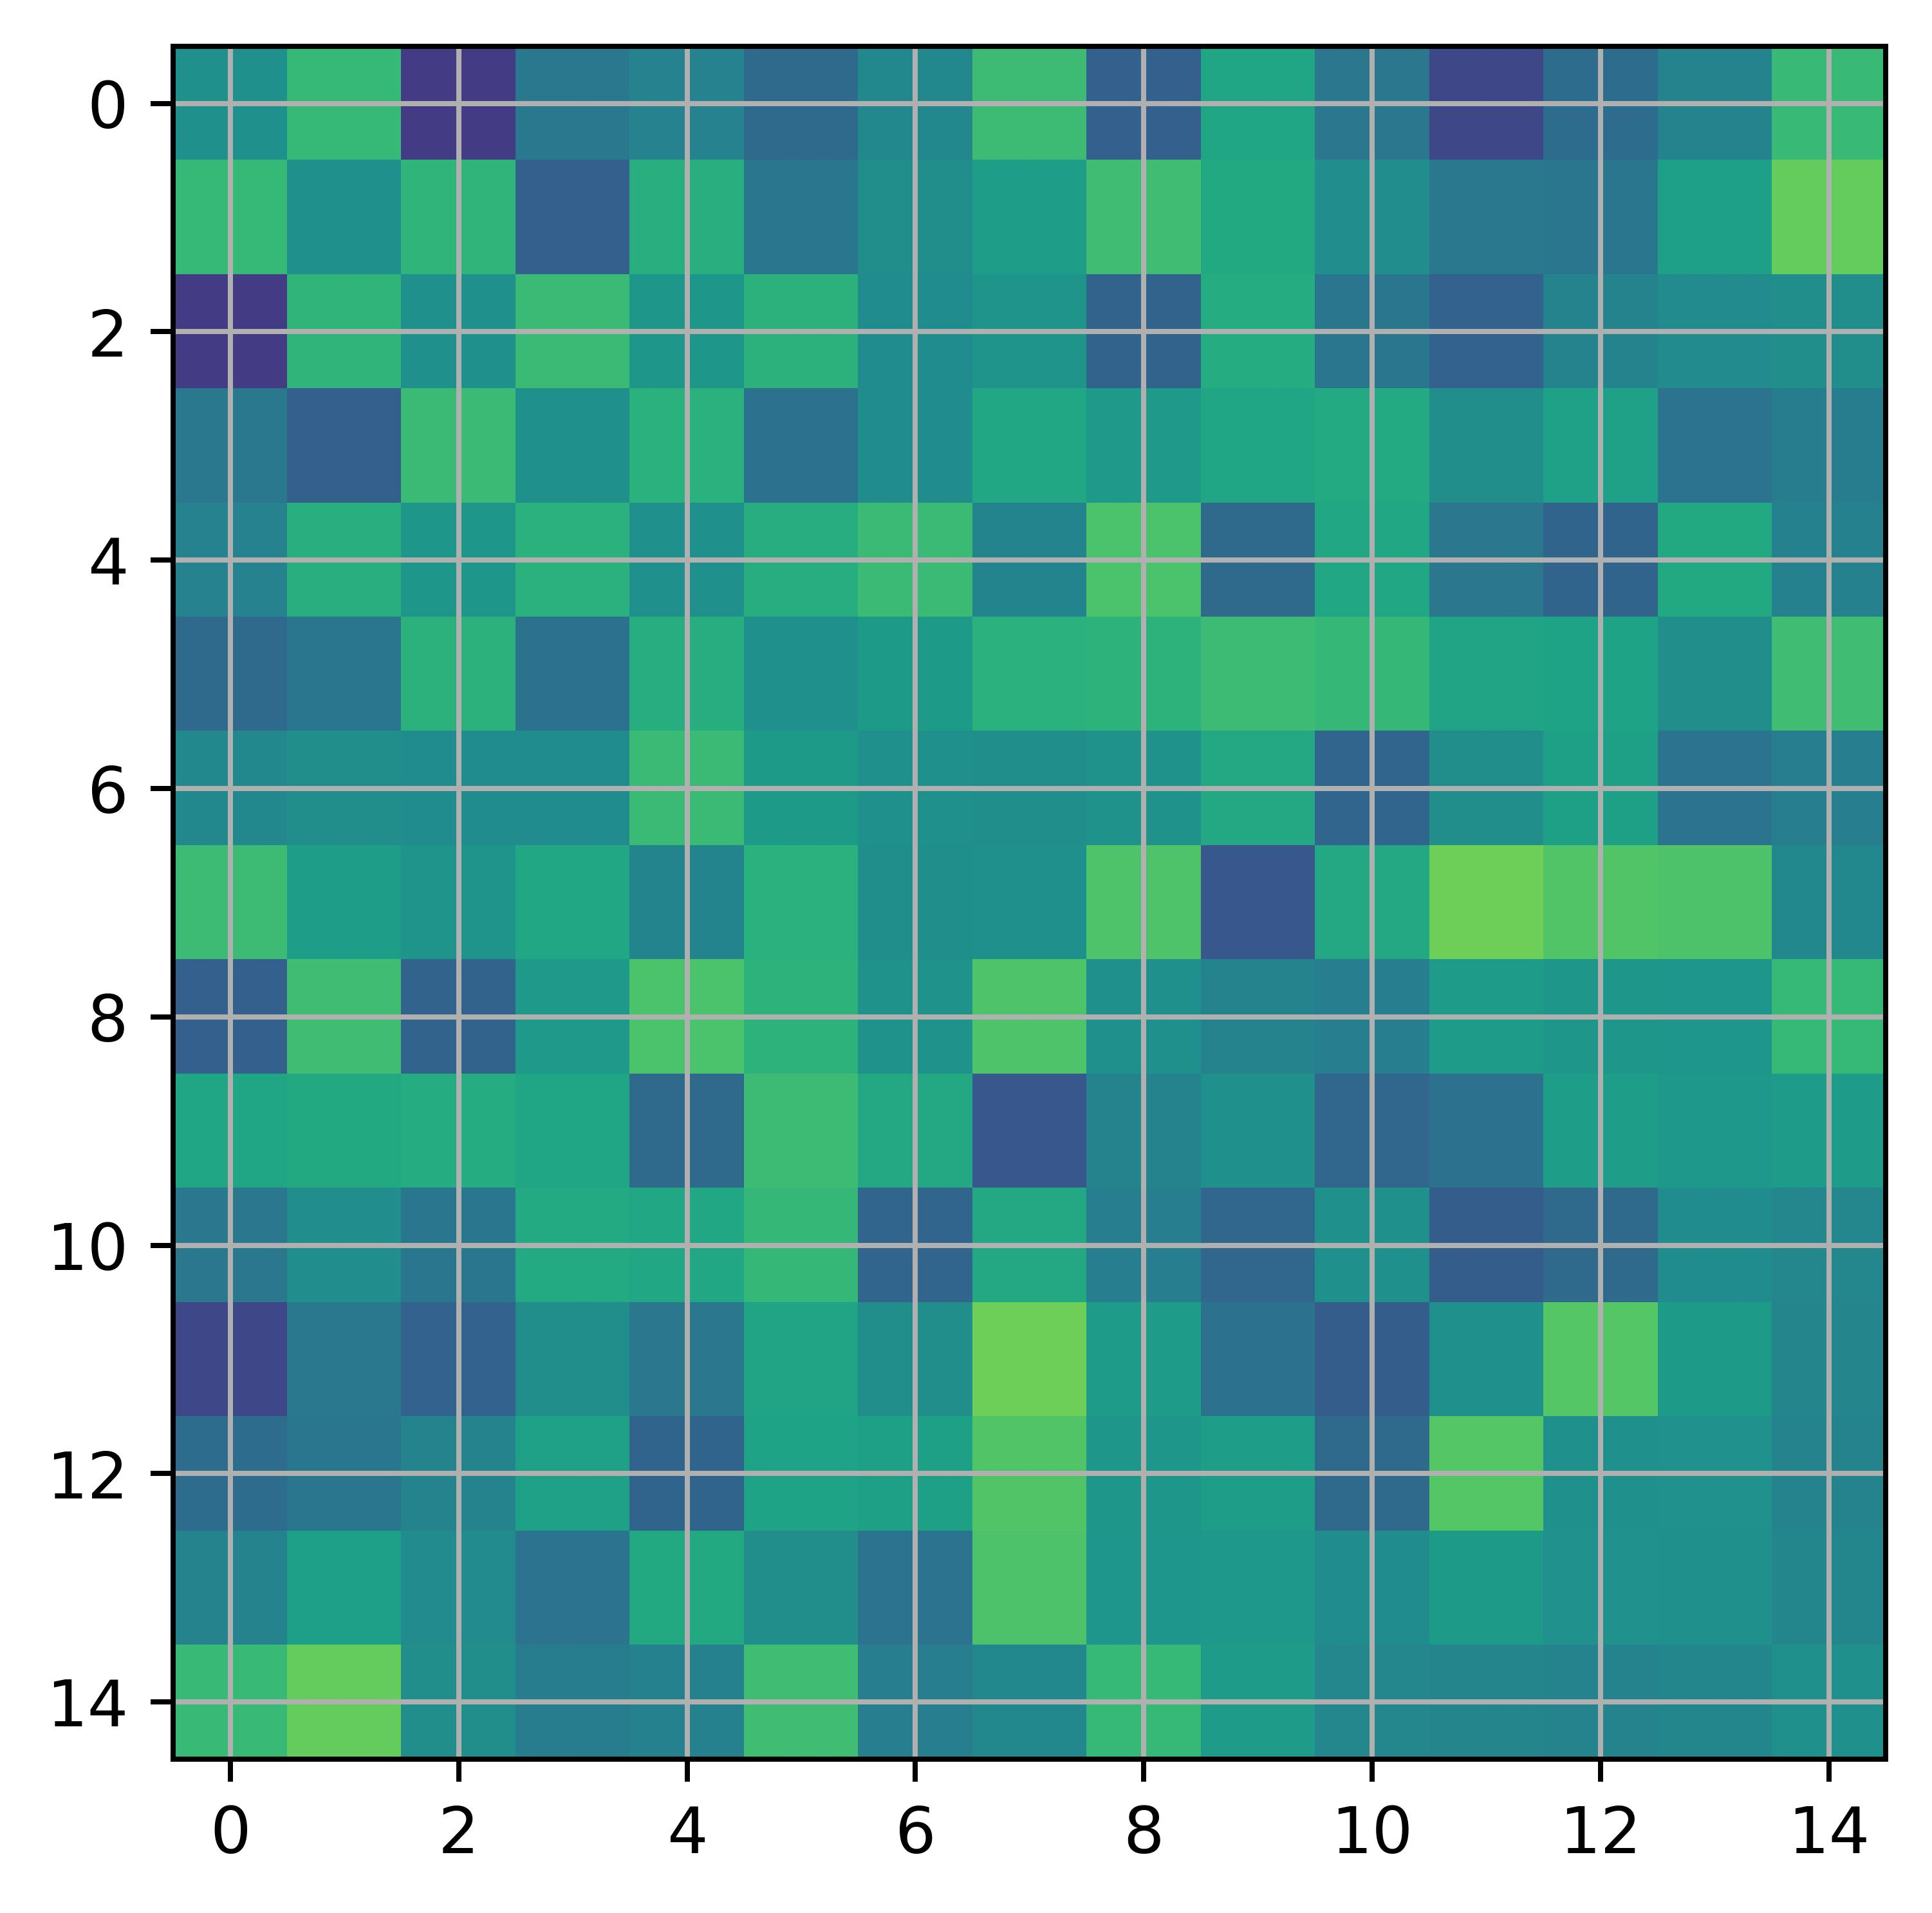
\includegraphics[width=0.18\textwidth]{../Analysis/DFC/size=480_step=180_rho=0.1/node=15_id=100206/n_c_0.jpg}
        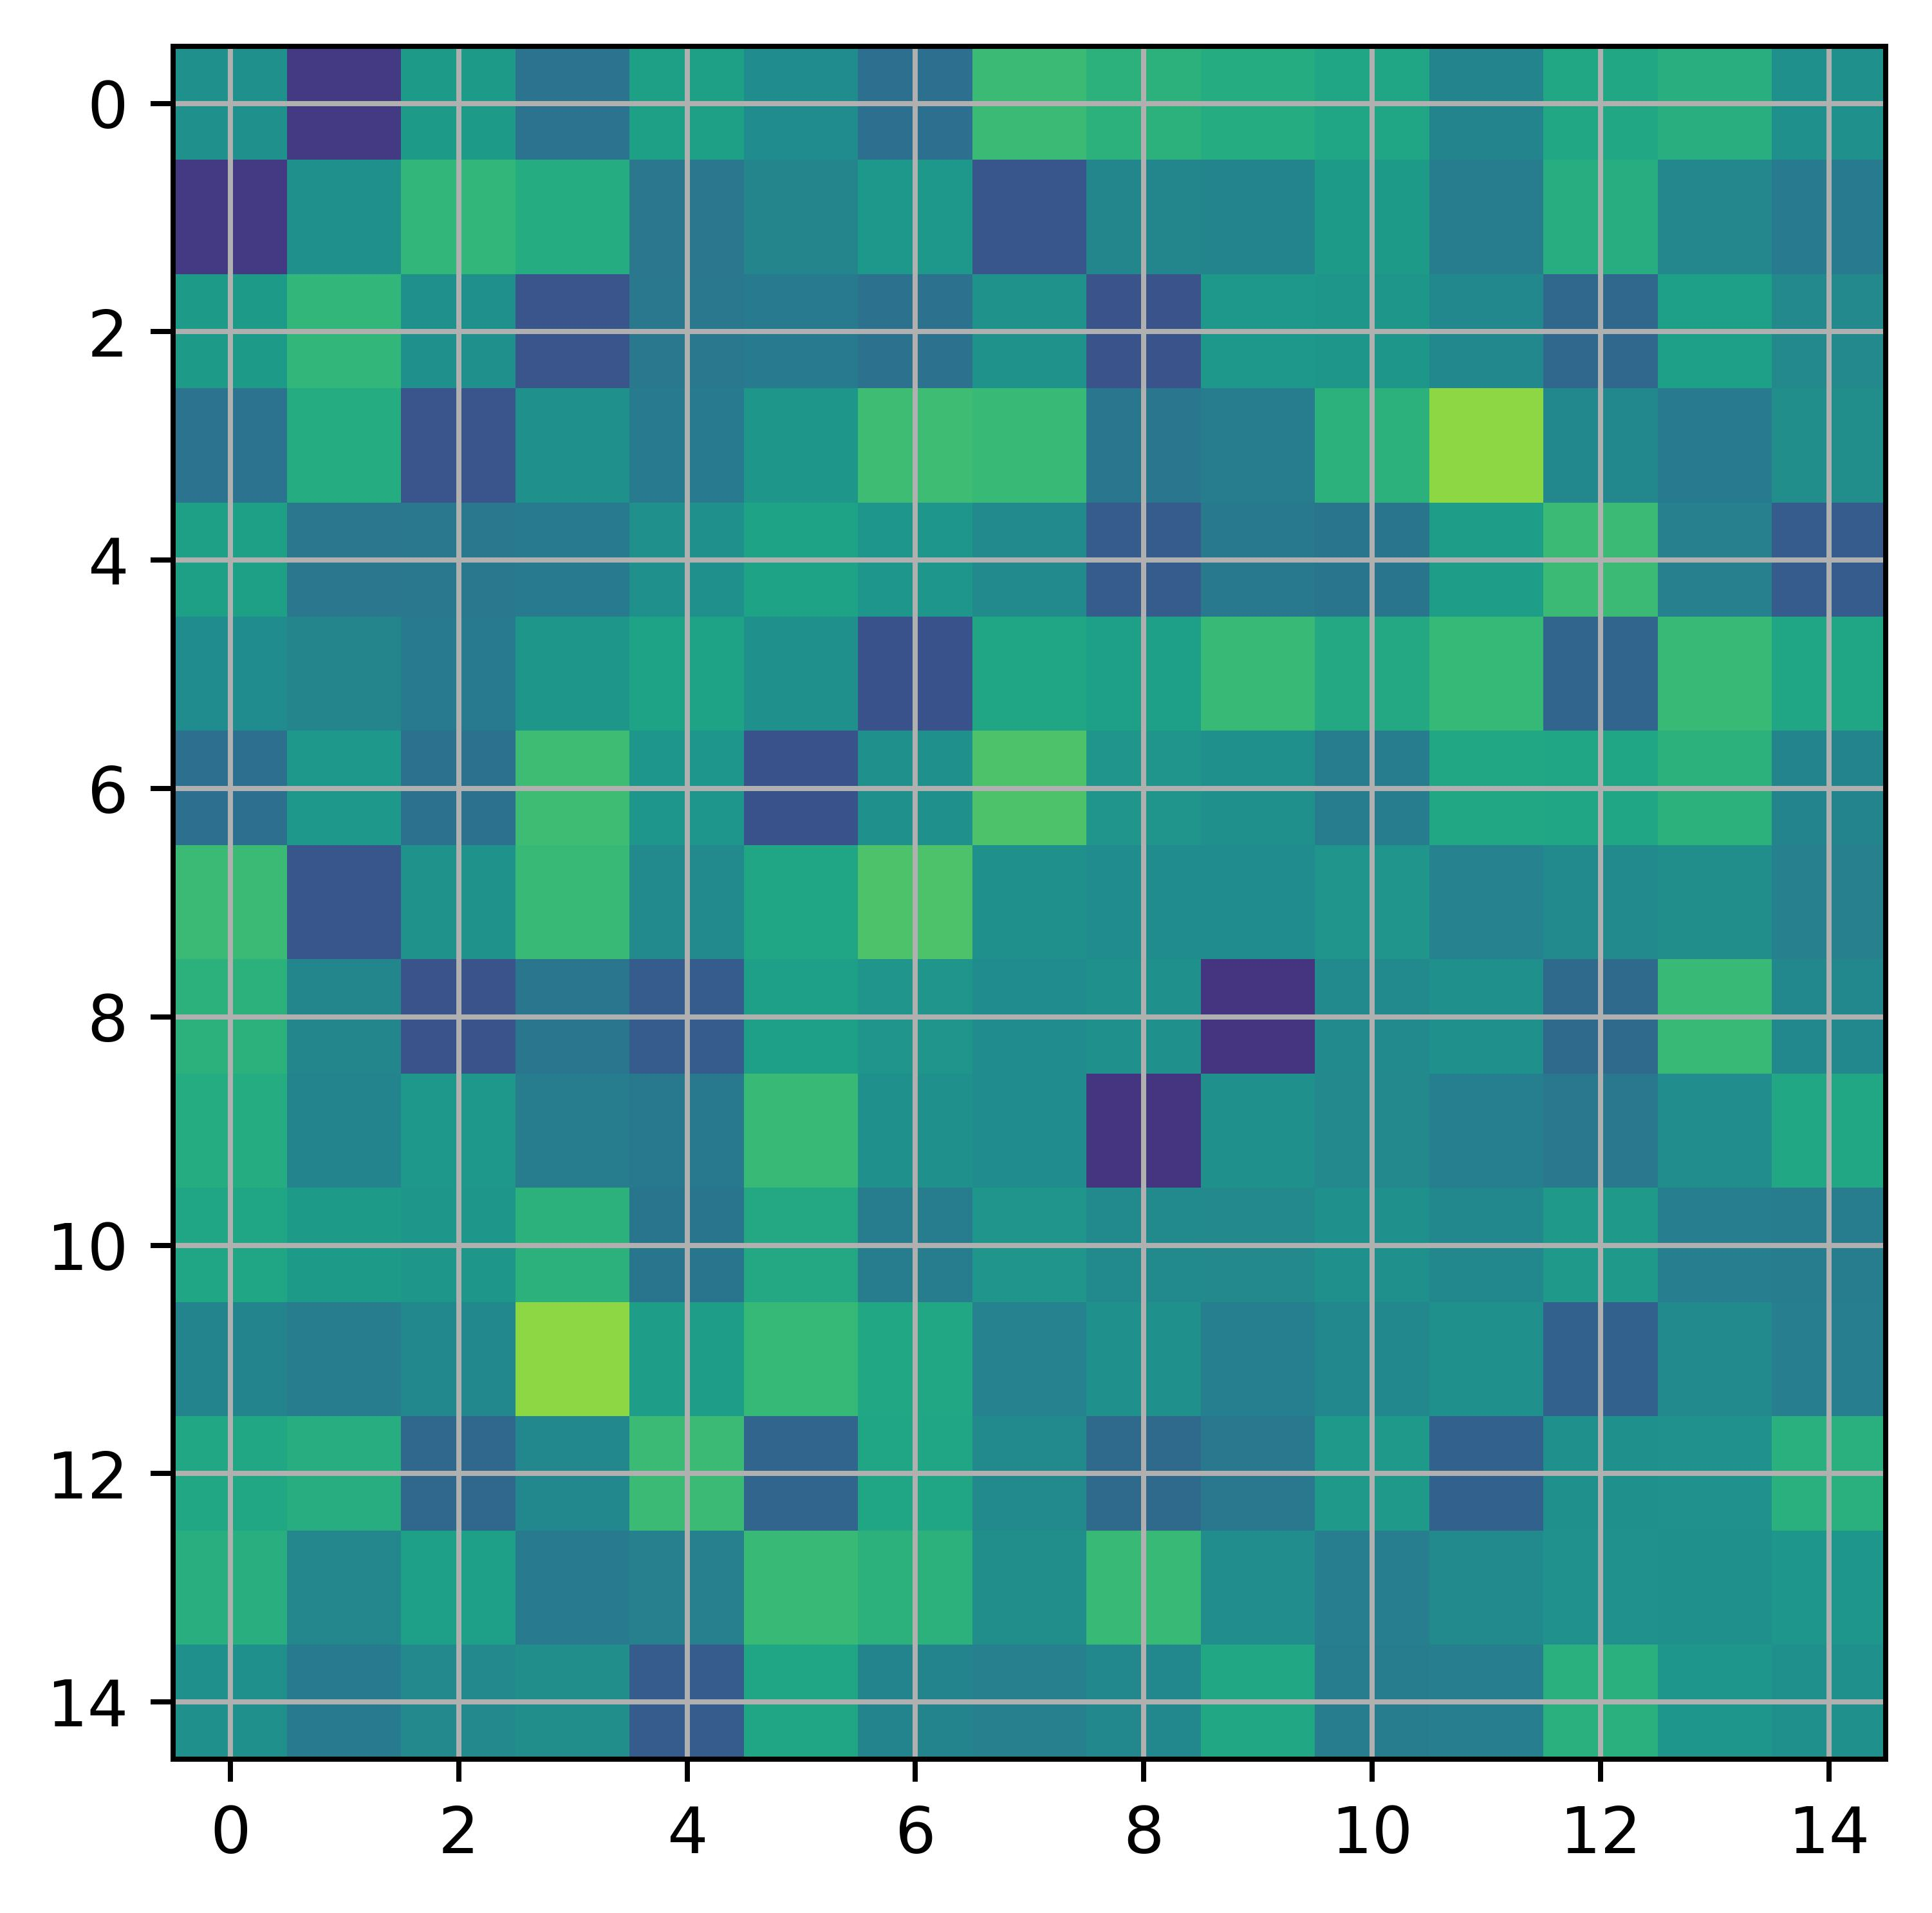
\includegraphics[width=0.18\textwidth]{../Analysis/DFC/size=480_step=180_rho=0.1/node=15_id=100206/n_c_6.jpg}
        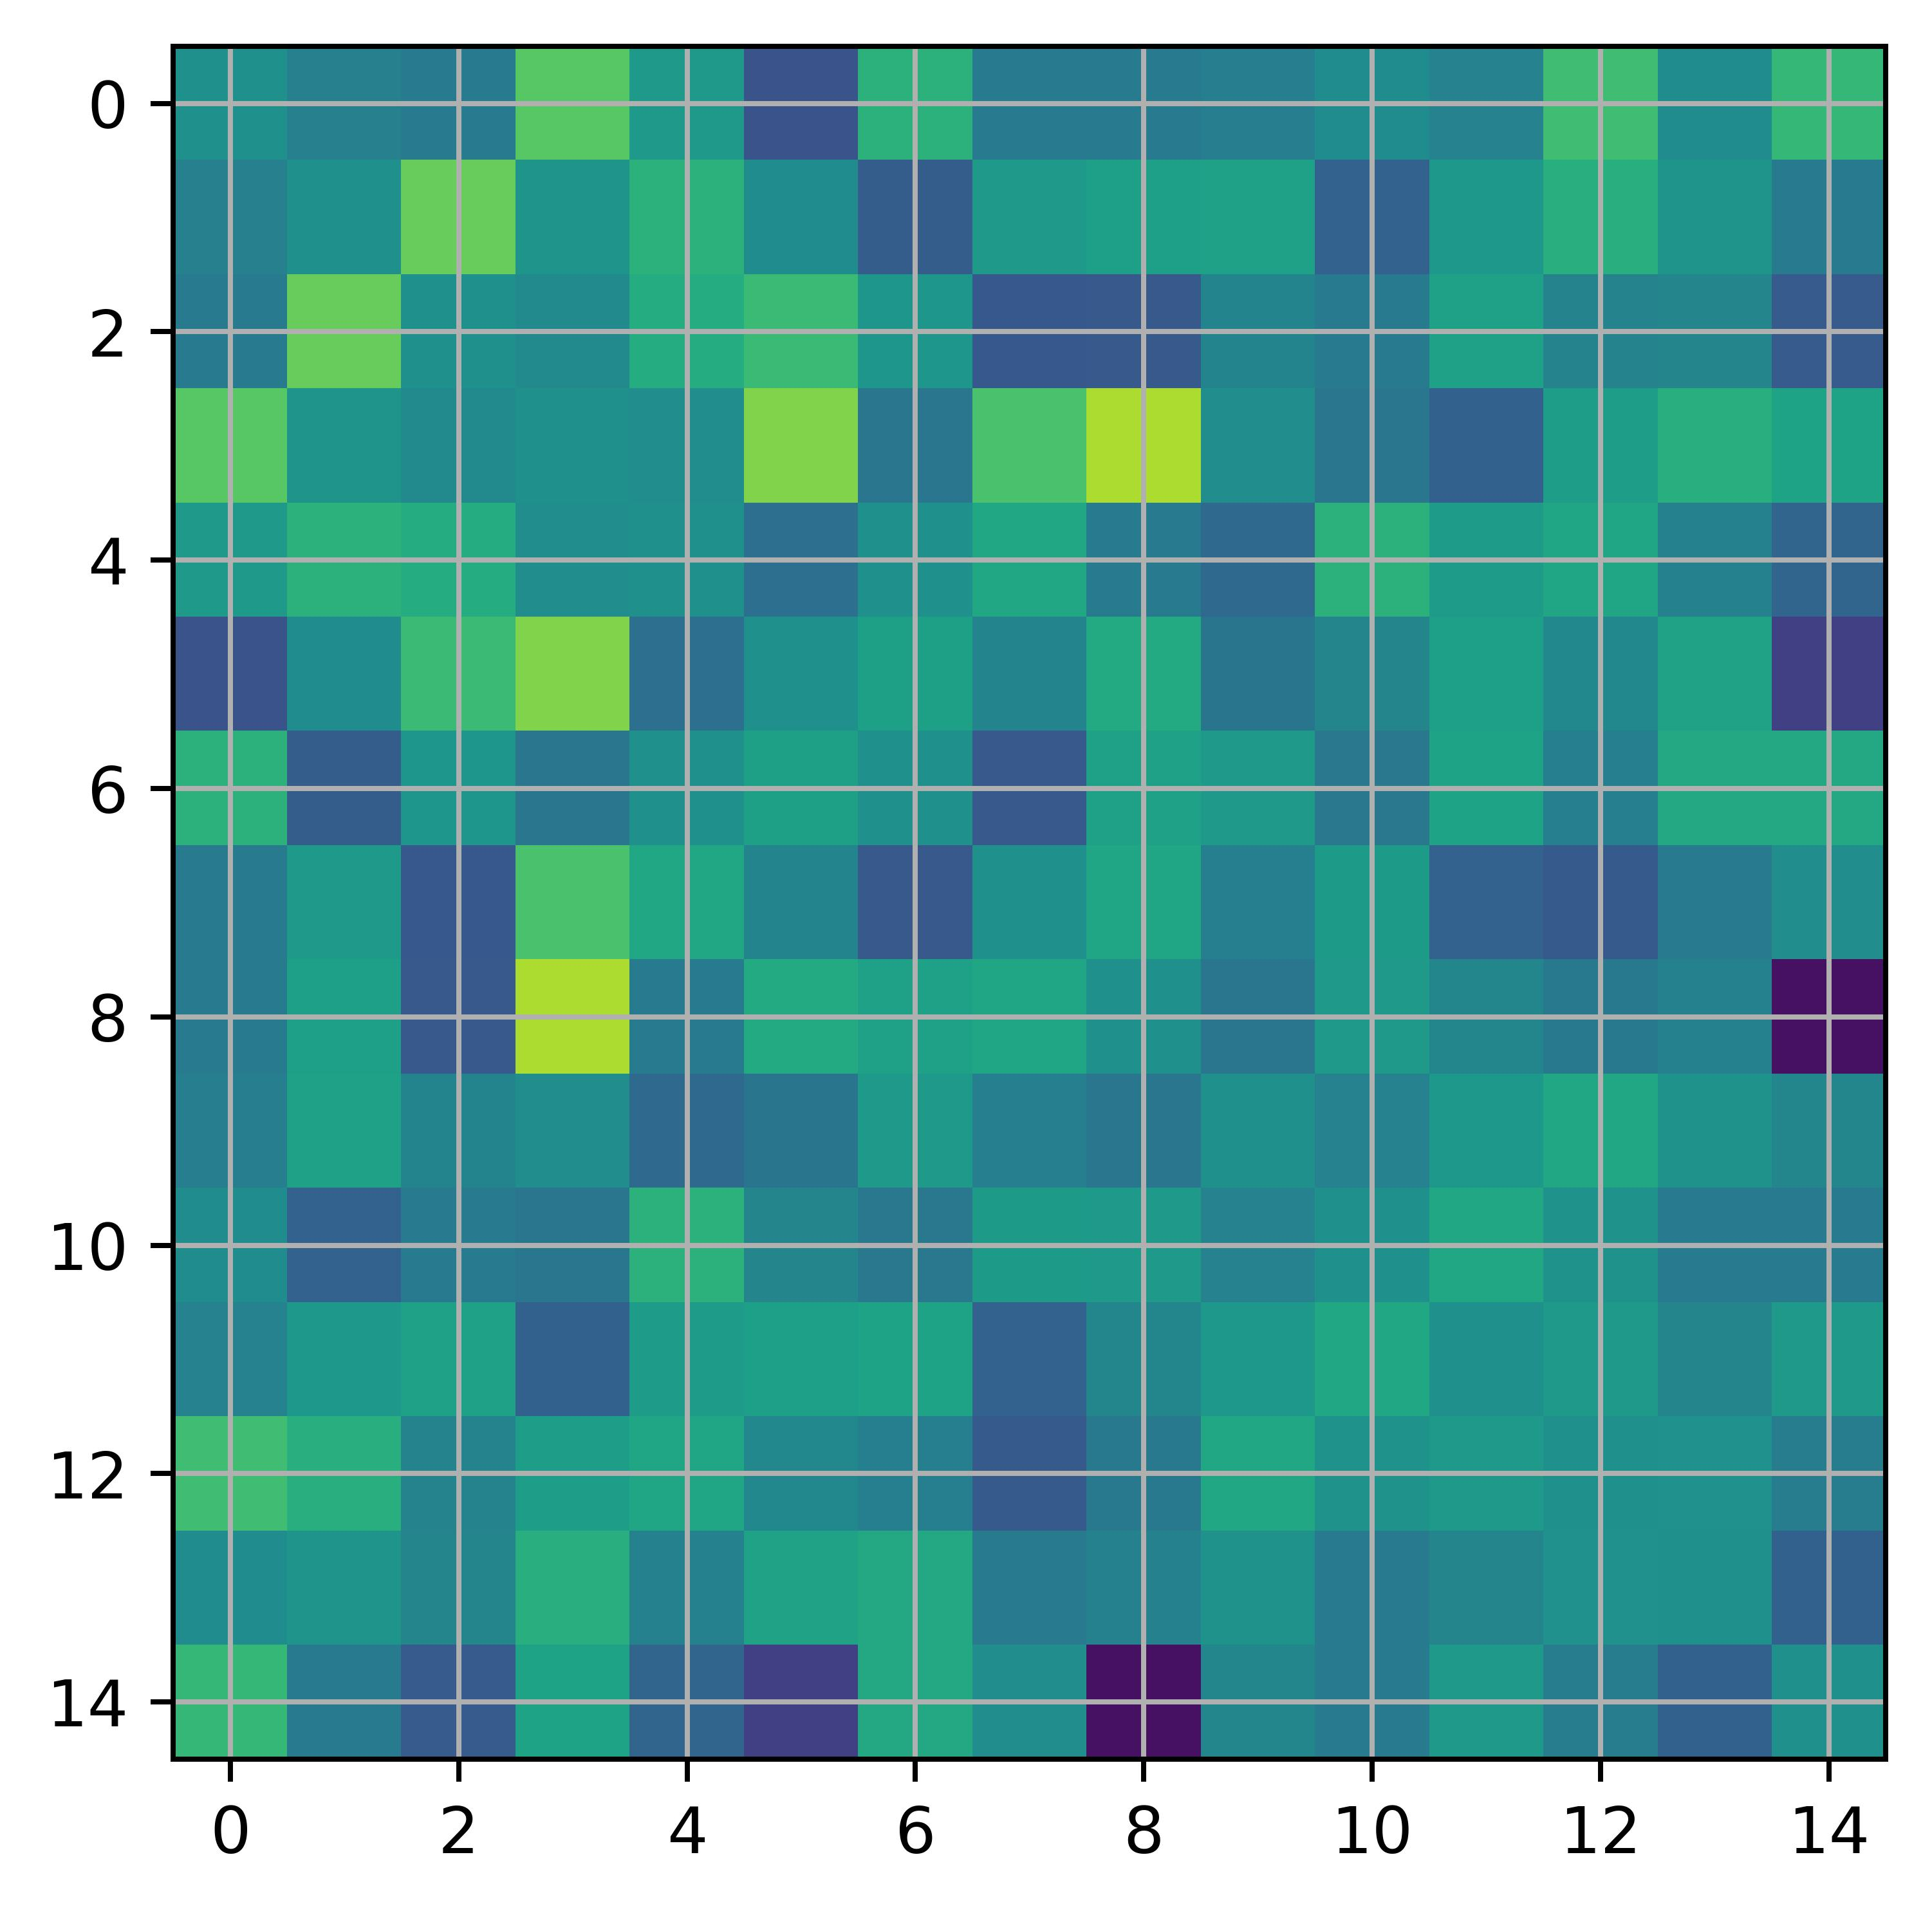
\includegraphics[width=0.18\textwidth]{../Analysis/DFC/size=480_step=180_rho=0.1/node=15_id=100206/n_c_12.jpg}
        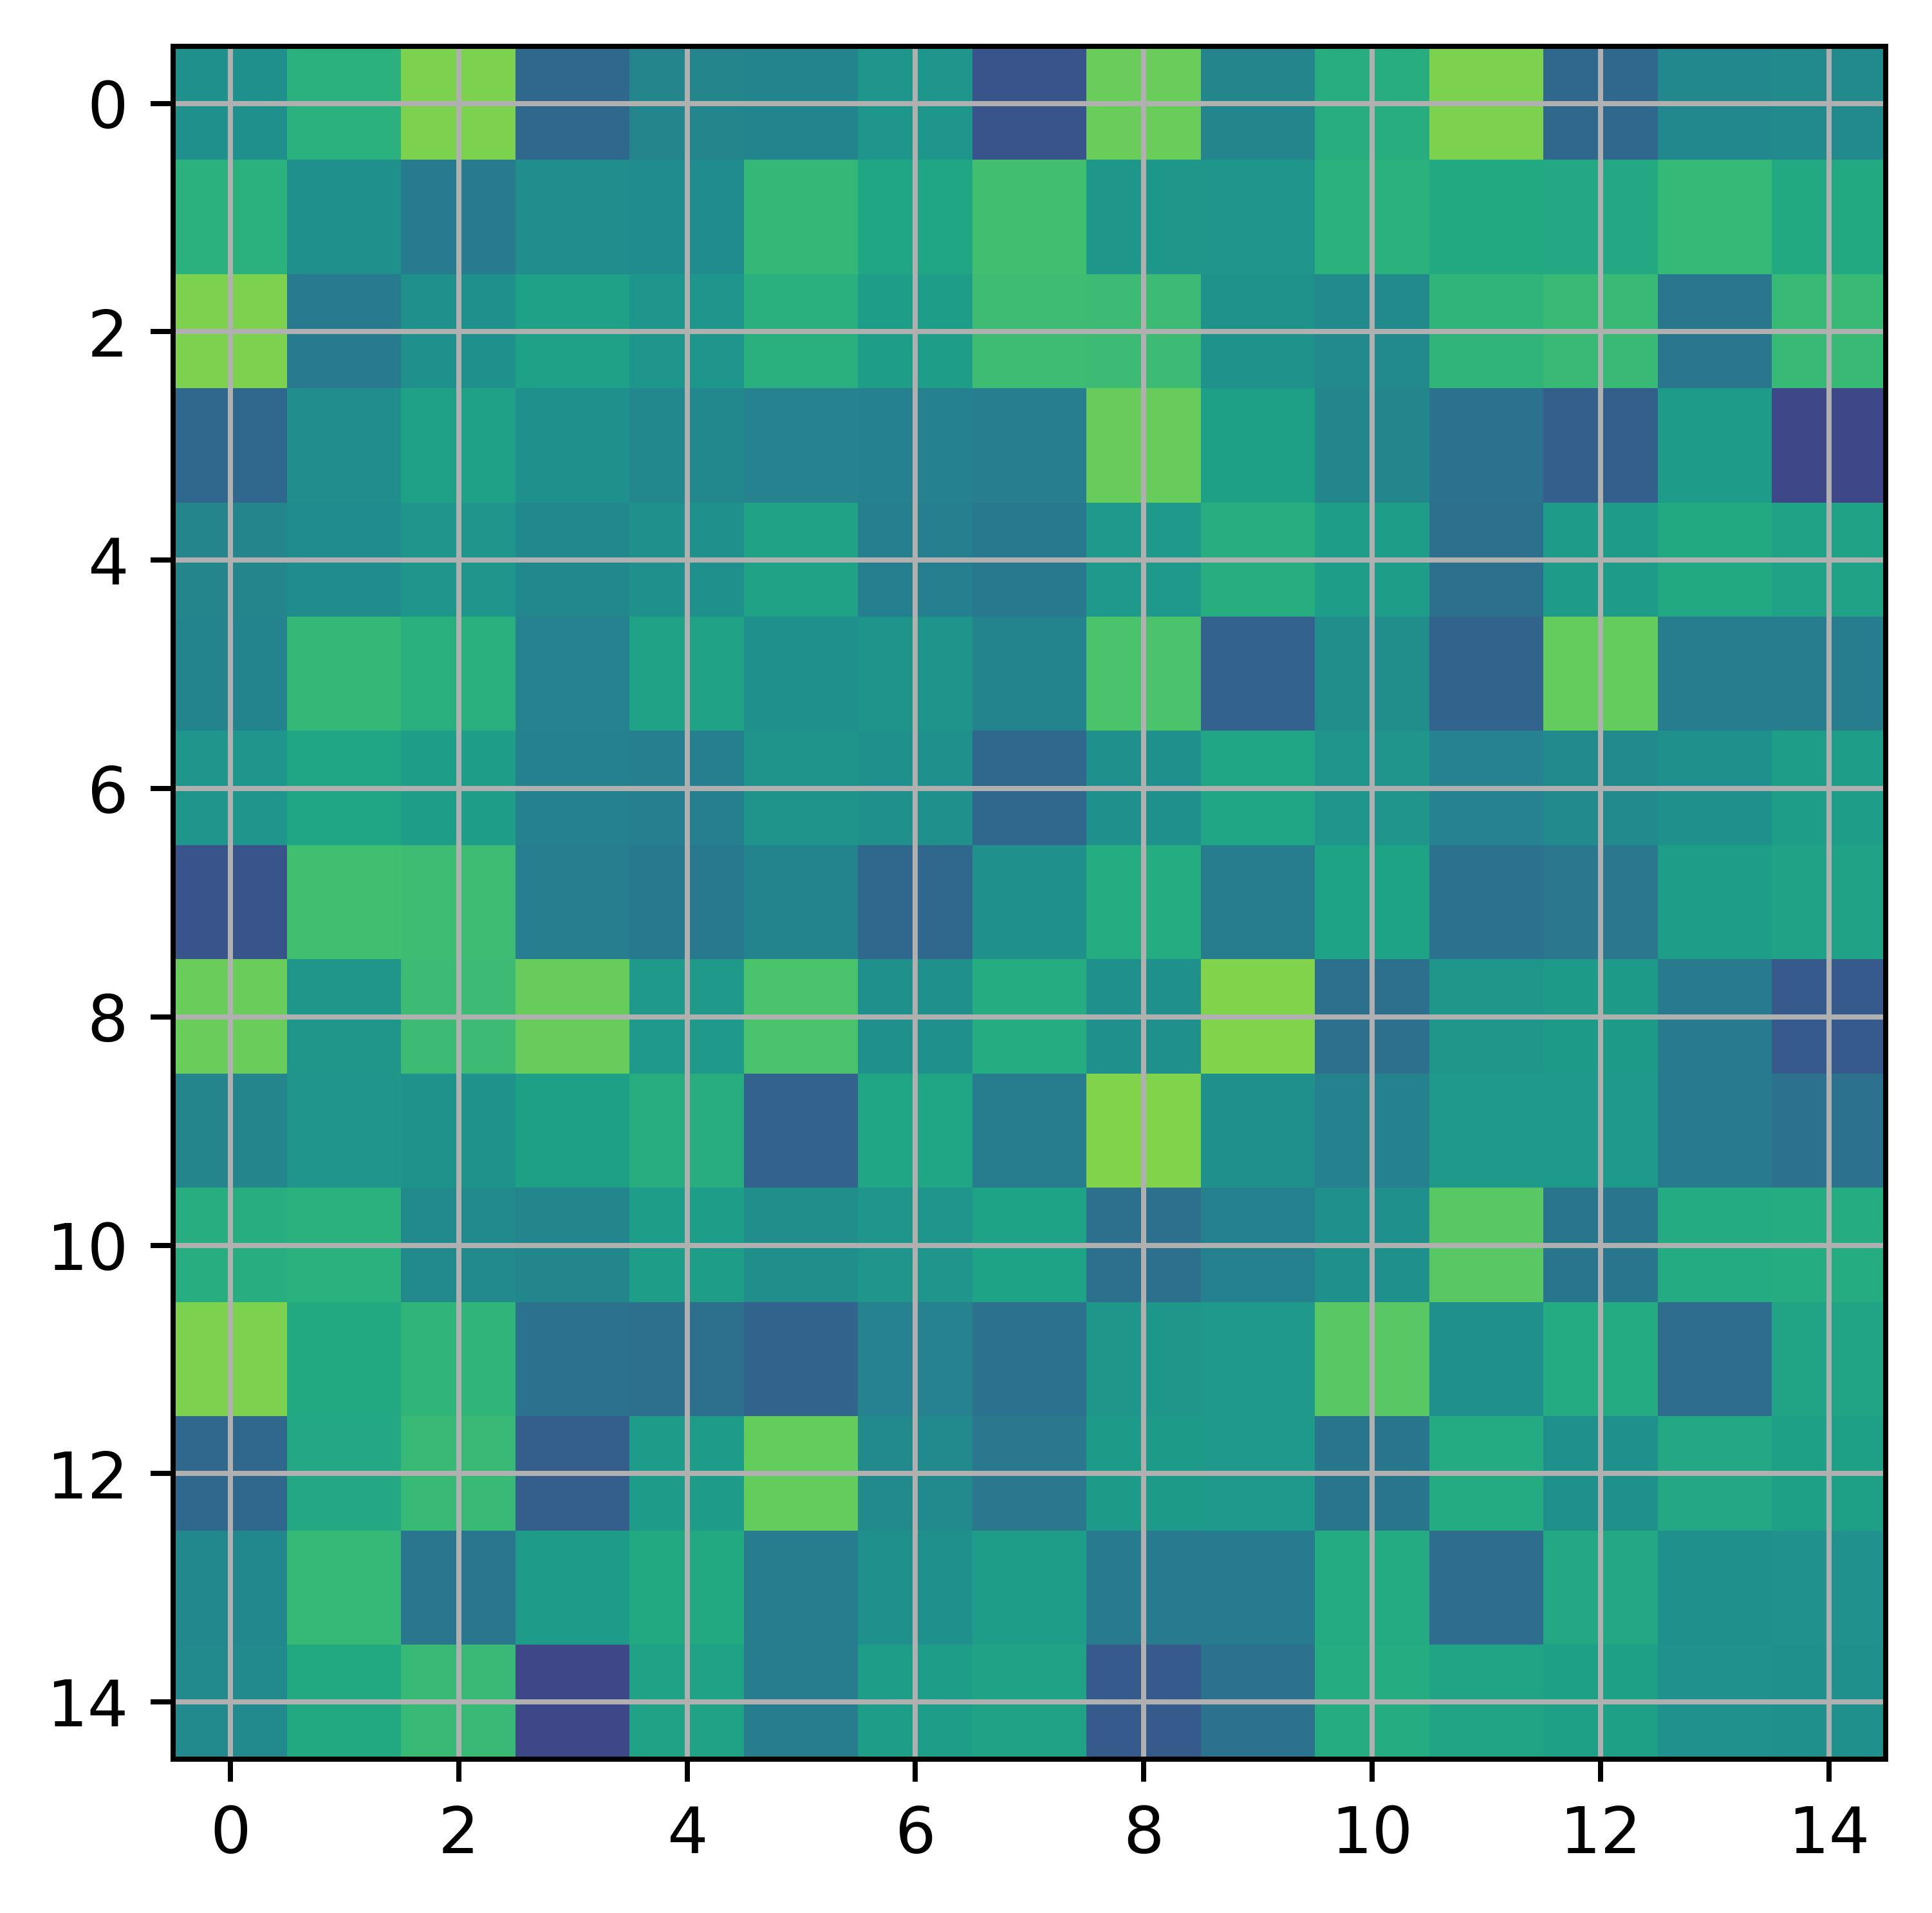
\includegraphics[width=0.18\textwidth]{../Analysis/DFC/size=480_step=180_rho=0.1/node=15_id=100206/n_c_18.jpg}
        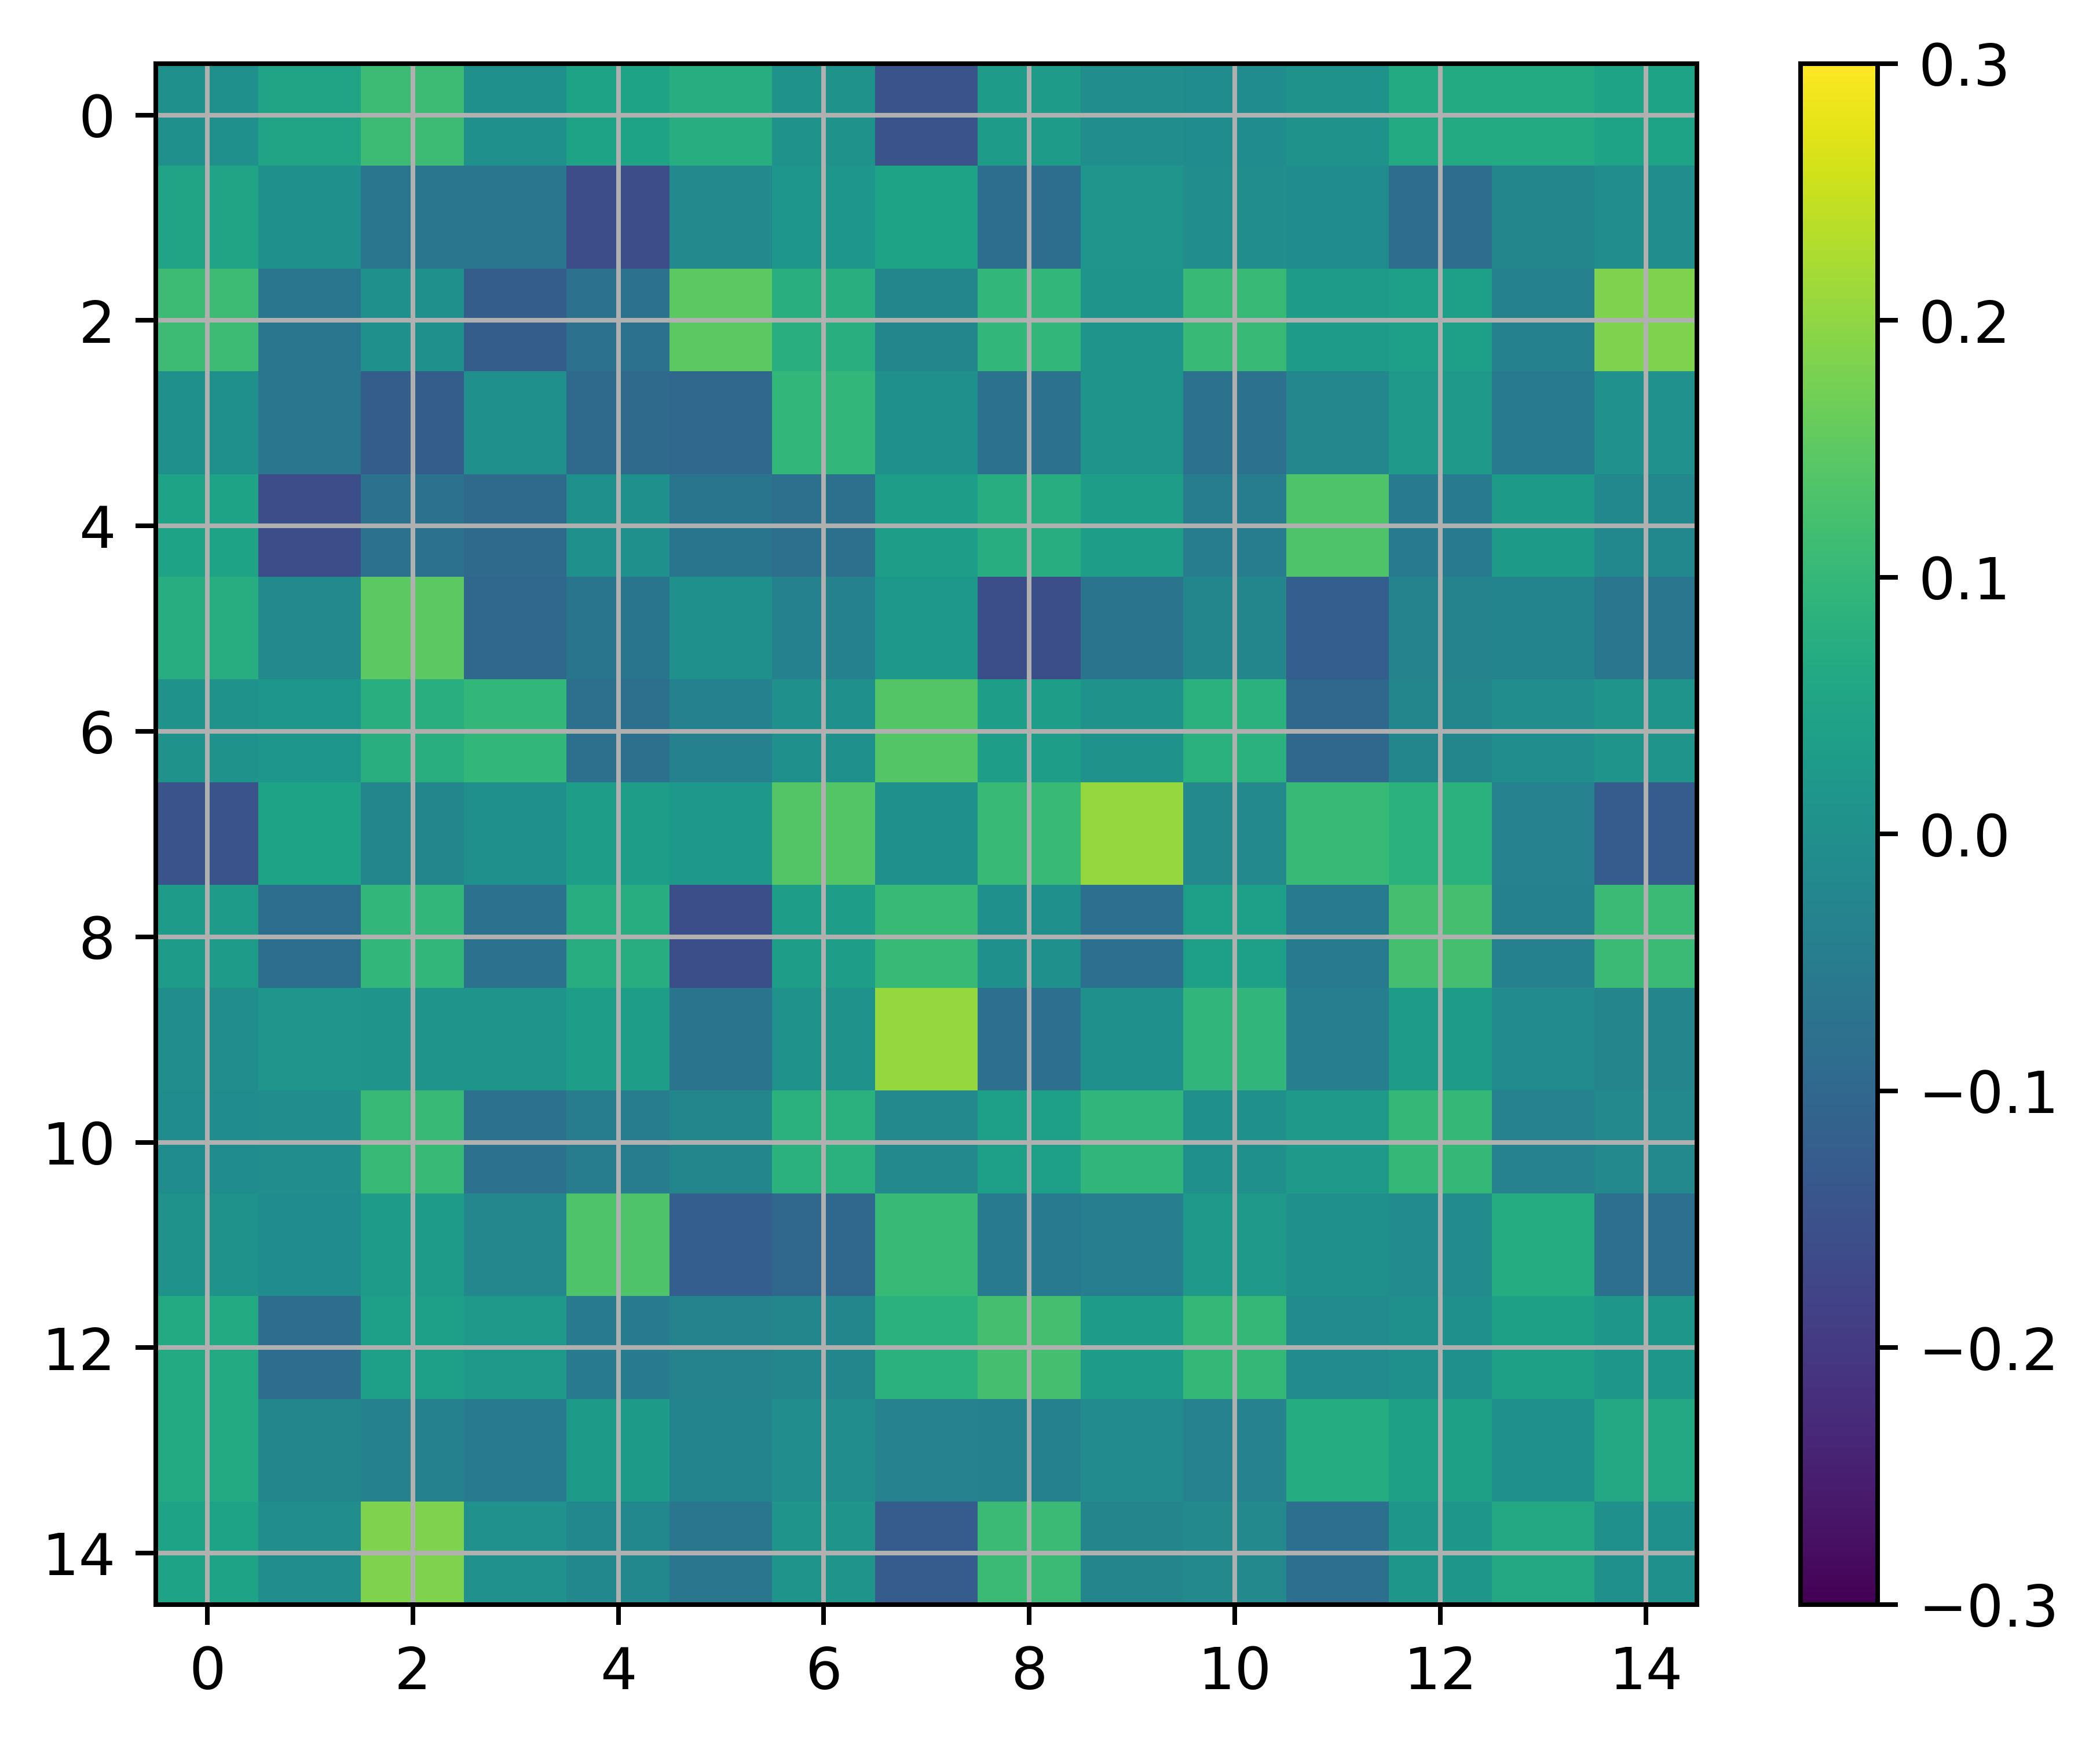
\includegraphics[width=0.2175\textwidth]{../Analysis/DFC/size=480_step=180_rho=0.1/node=15_id=100206/c_24.jpg}} \\
    \subfloat[$N_{\text{node}} = 25$]{
        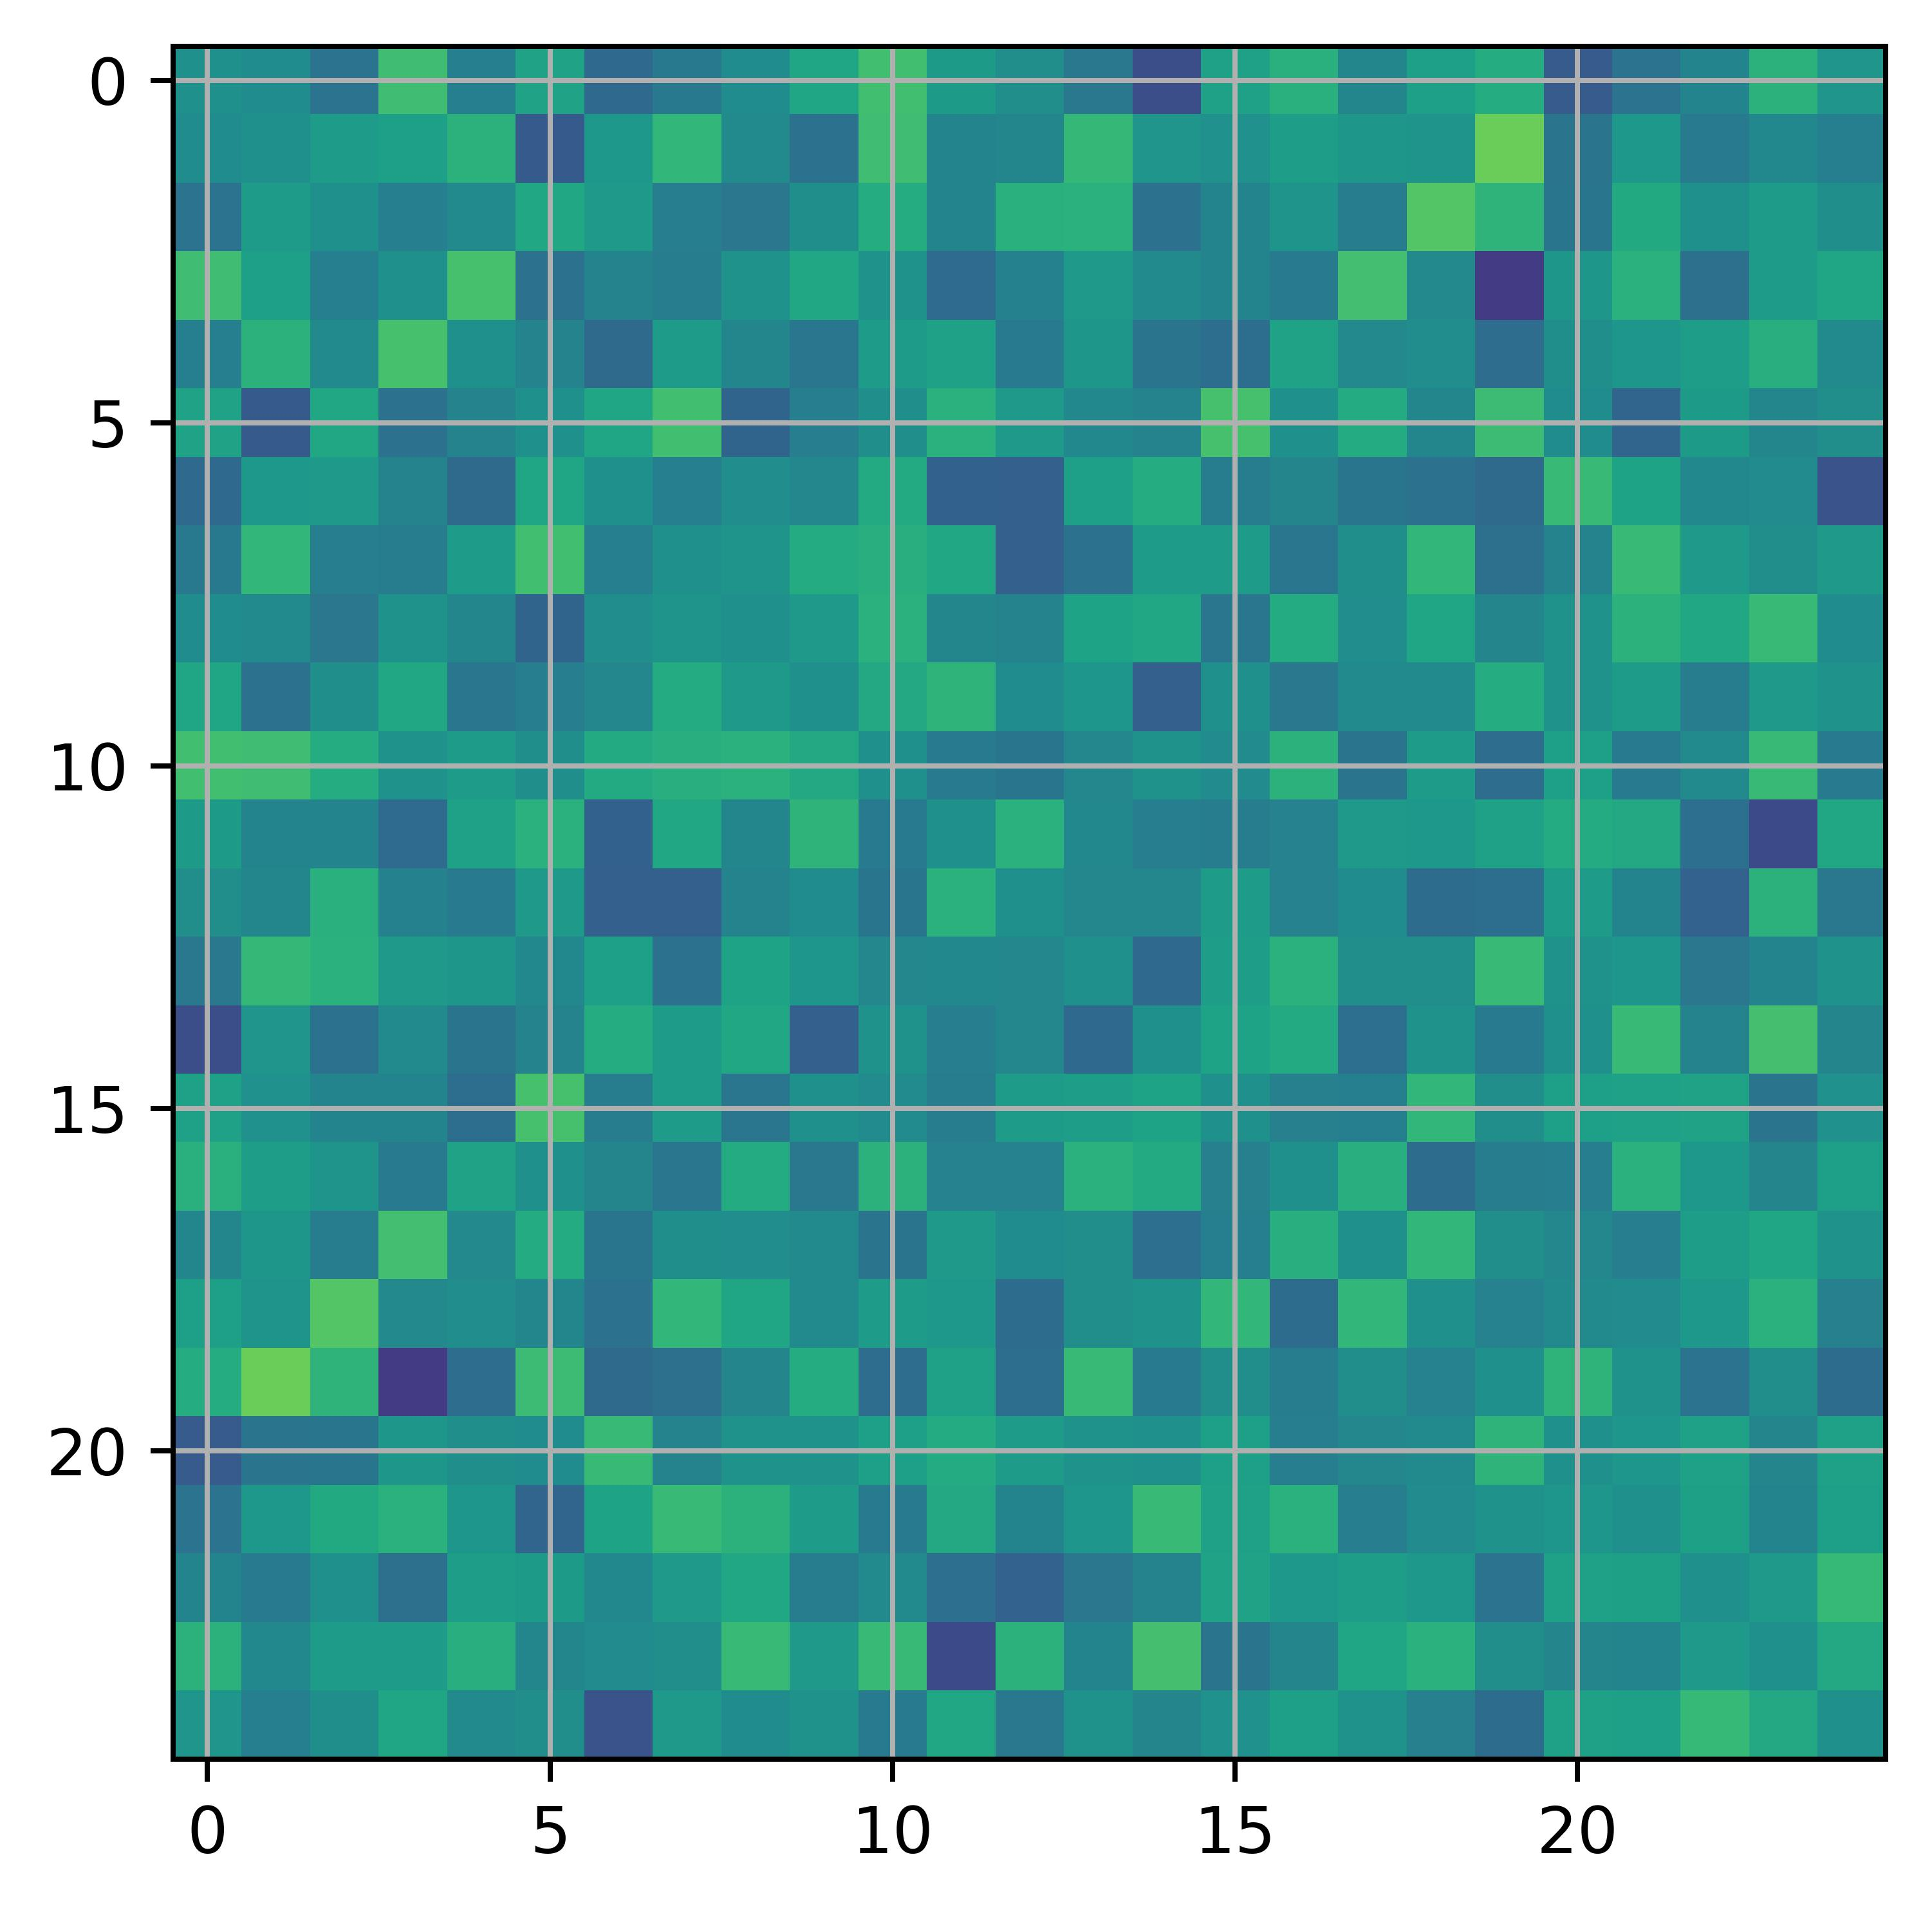
\includegraphics[width=0.18\textwidth]{../Analysis/DFC/size=480_step=180_rho=0.1/node=25_id=100206/n_c_0.jpg}
        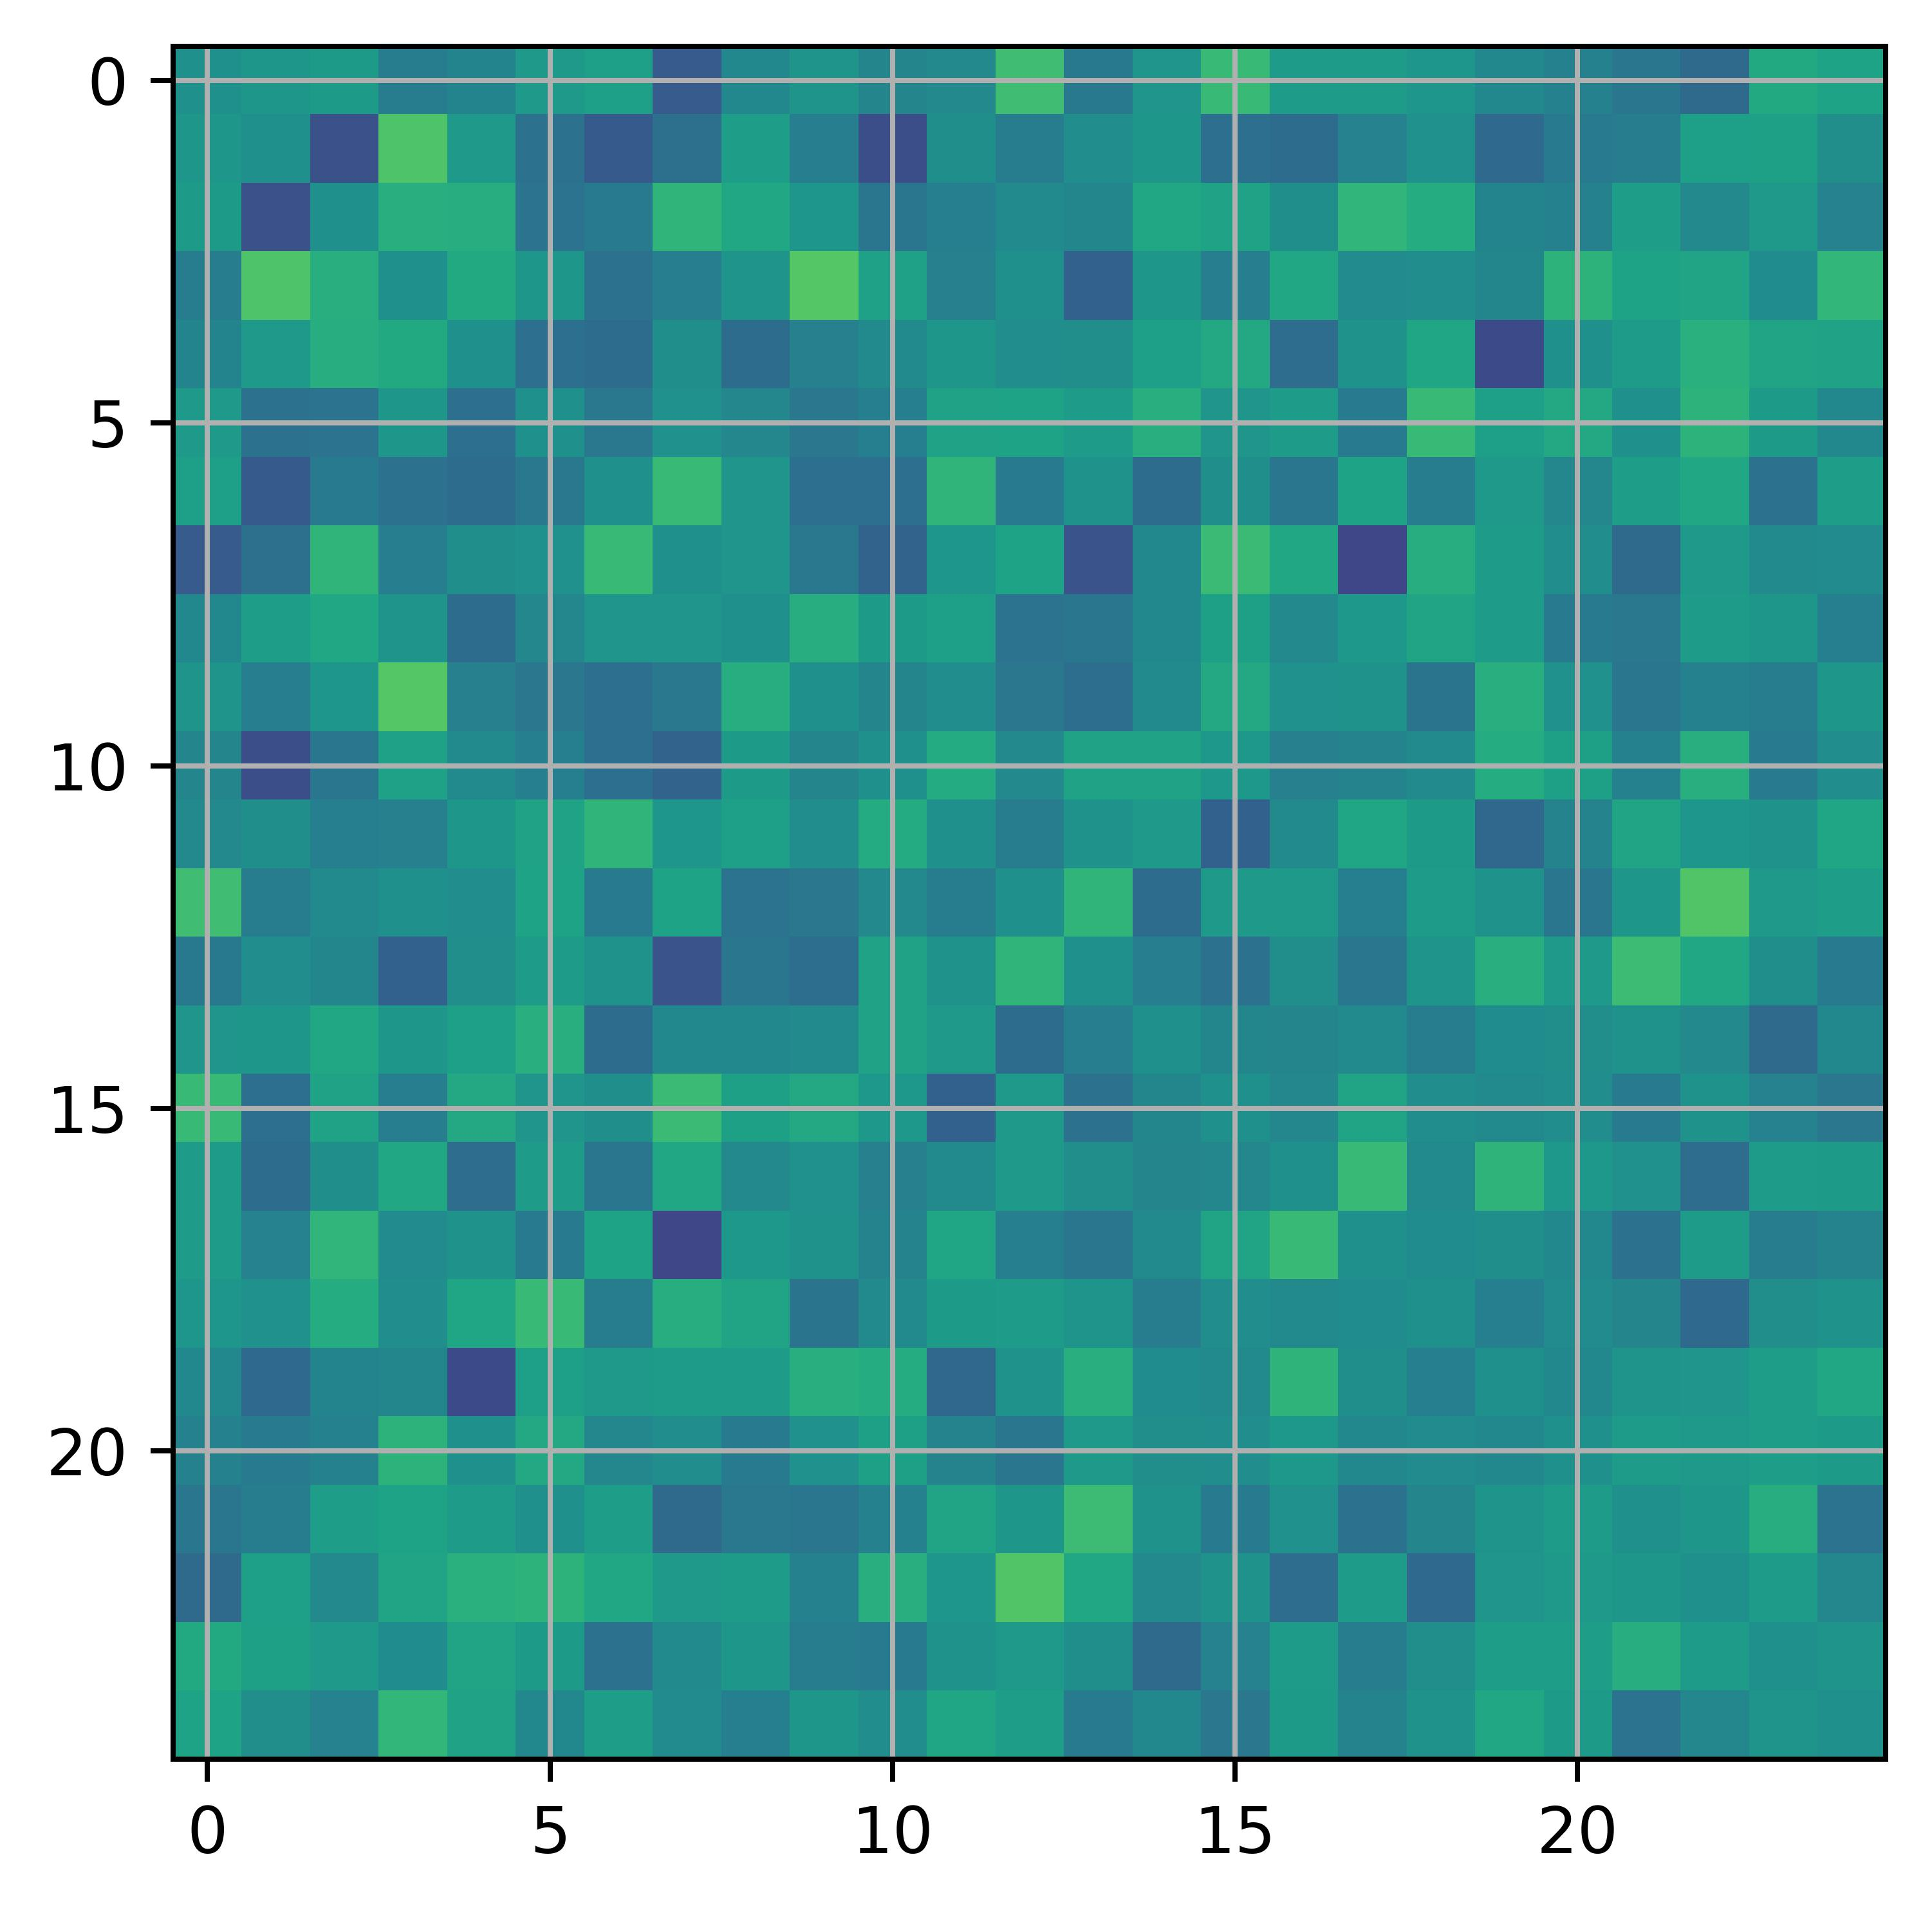
\includegraphics[width=0.18\textwidth]{../Analysis/DFC/size=480_step=180_rho=0.1/node=25_id=100206/n_c_6.jpg}
        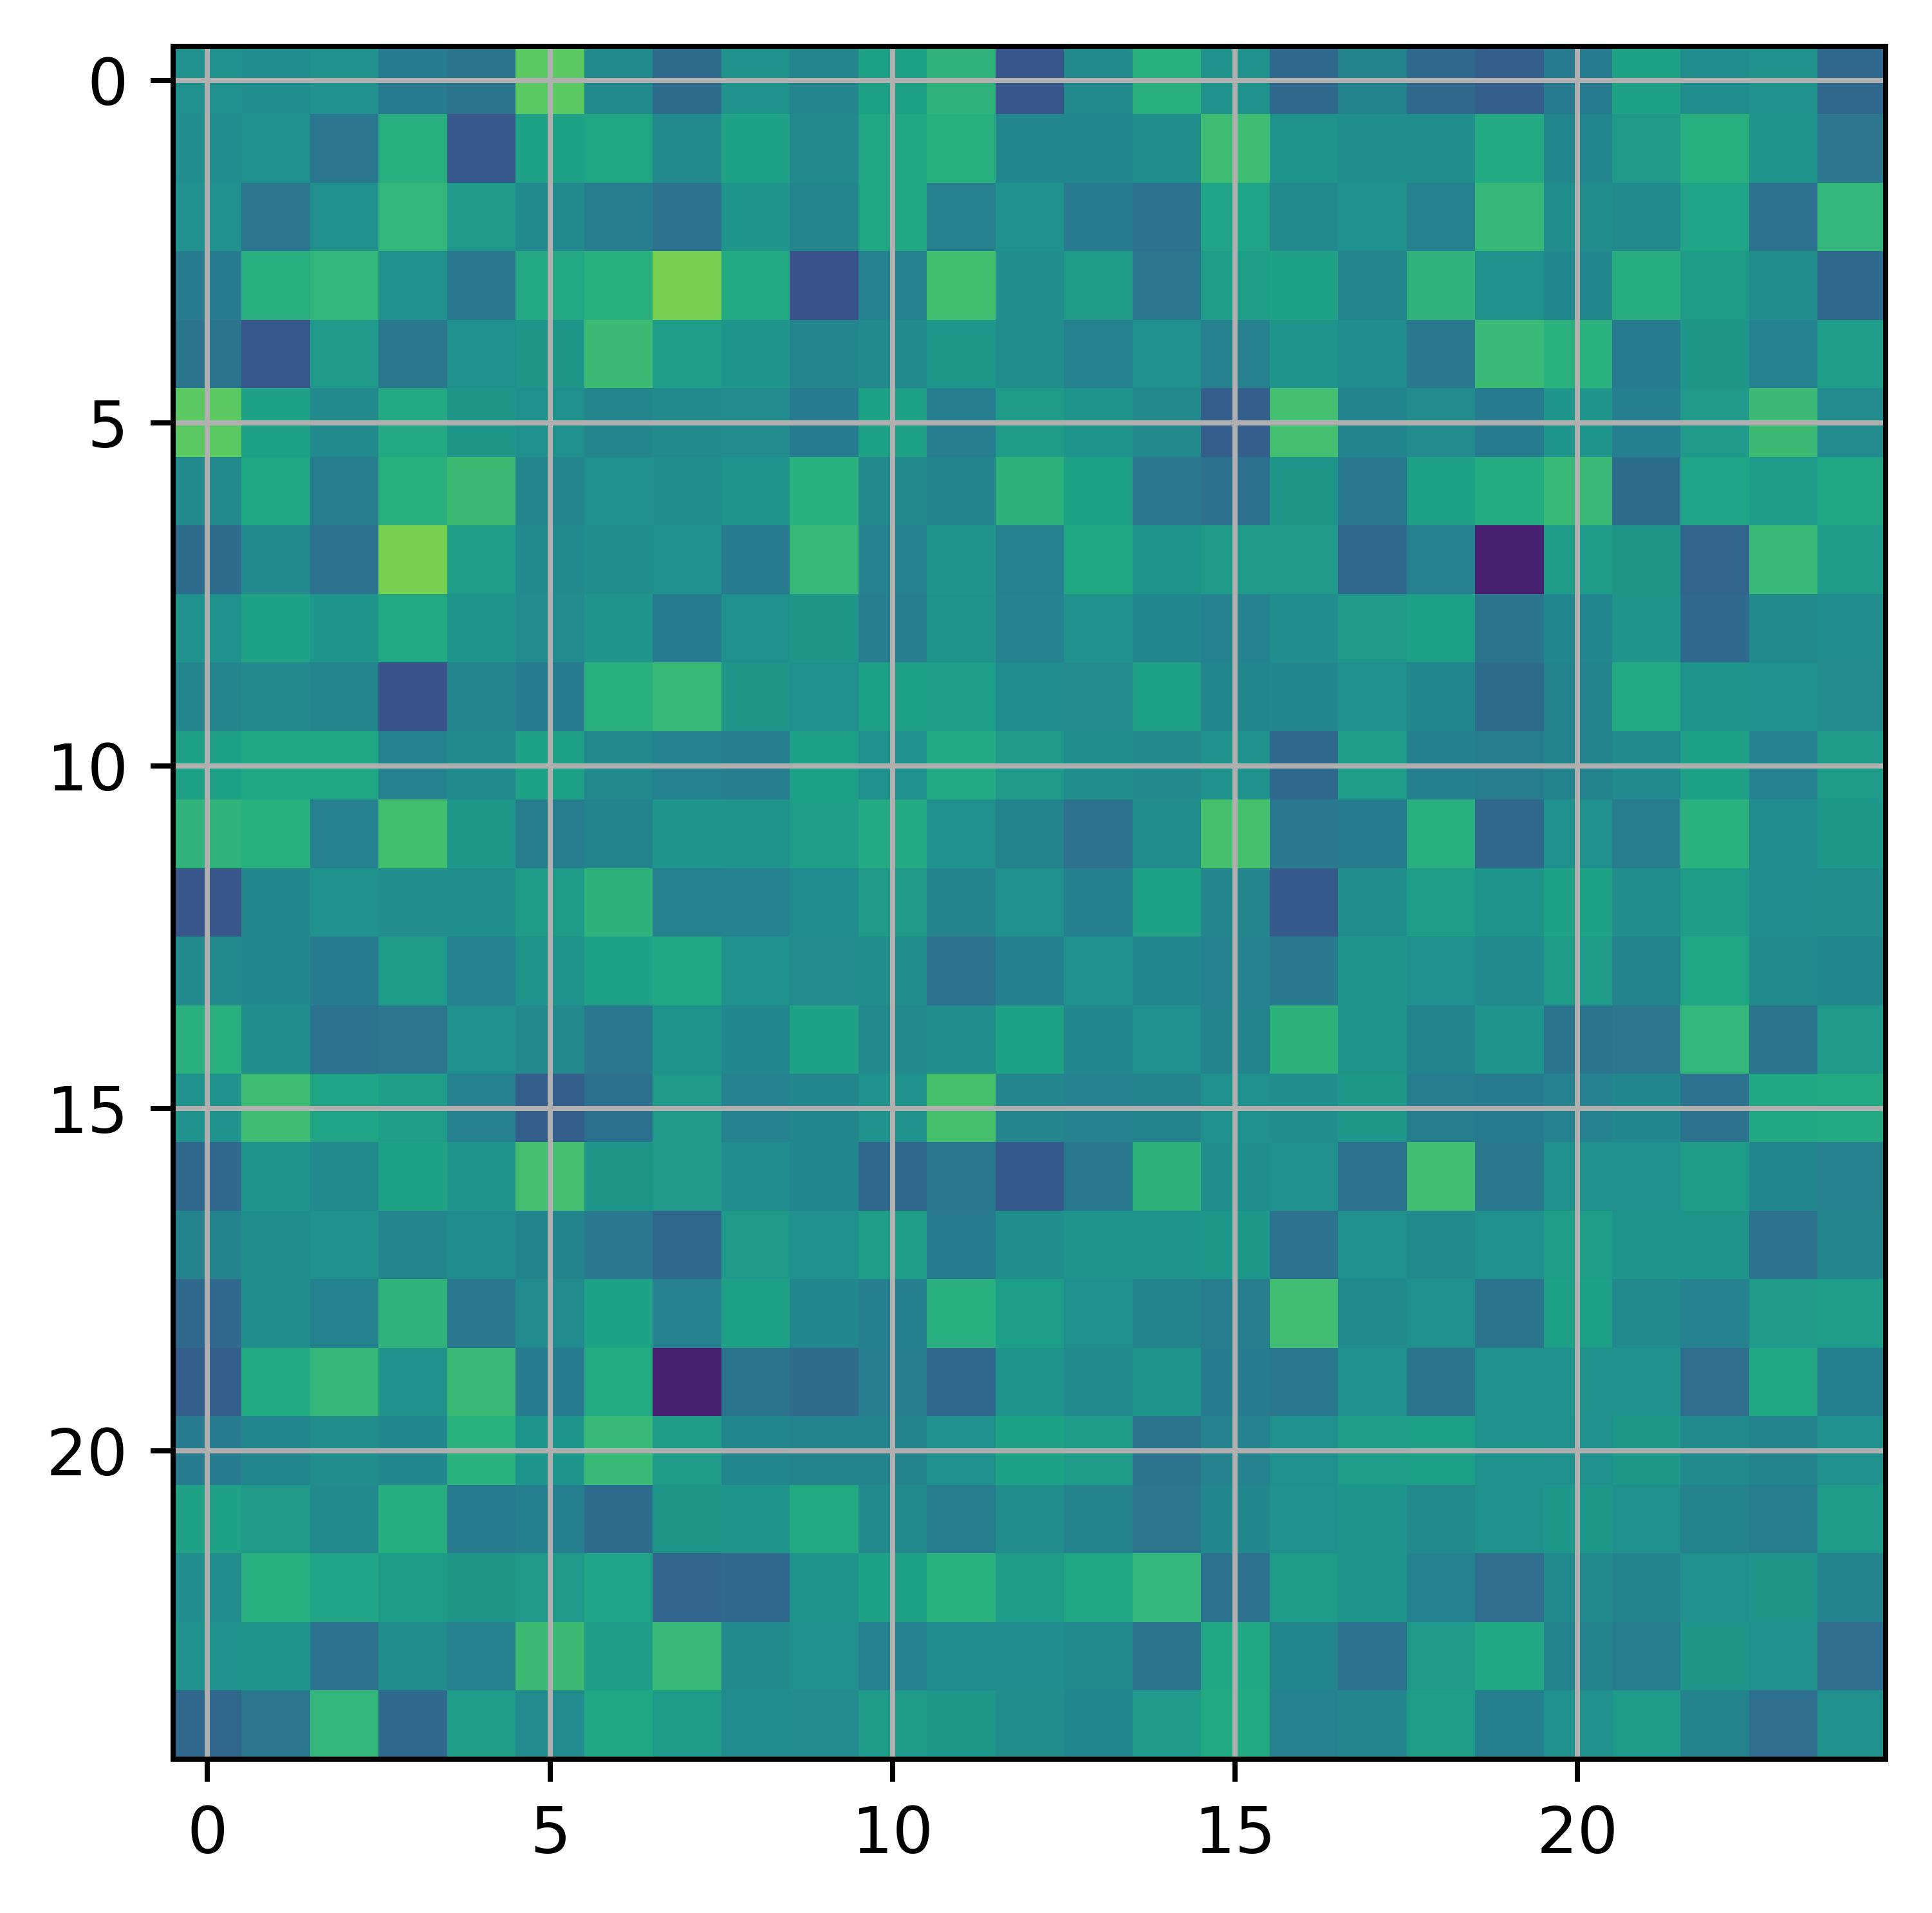
\includegraphics[width=0.18\textwidth]{../Analysis/DFC/size=480_step=180_rho=0.1/node=25_id=100206/n_c_12.jpg}
        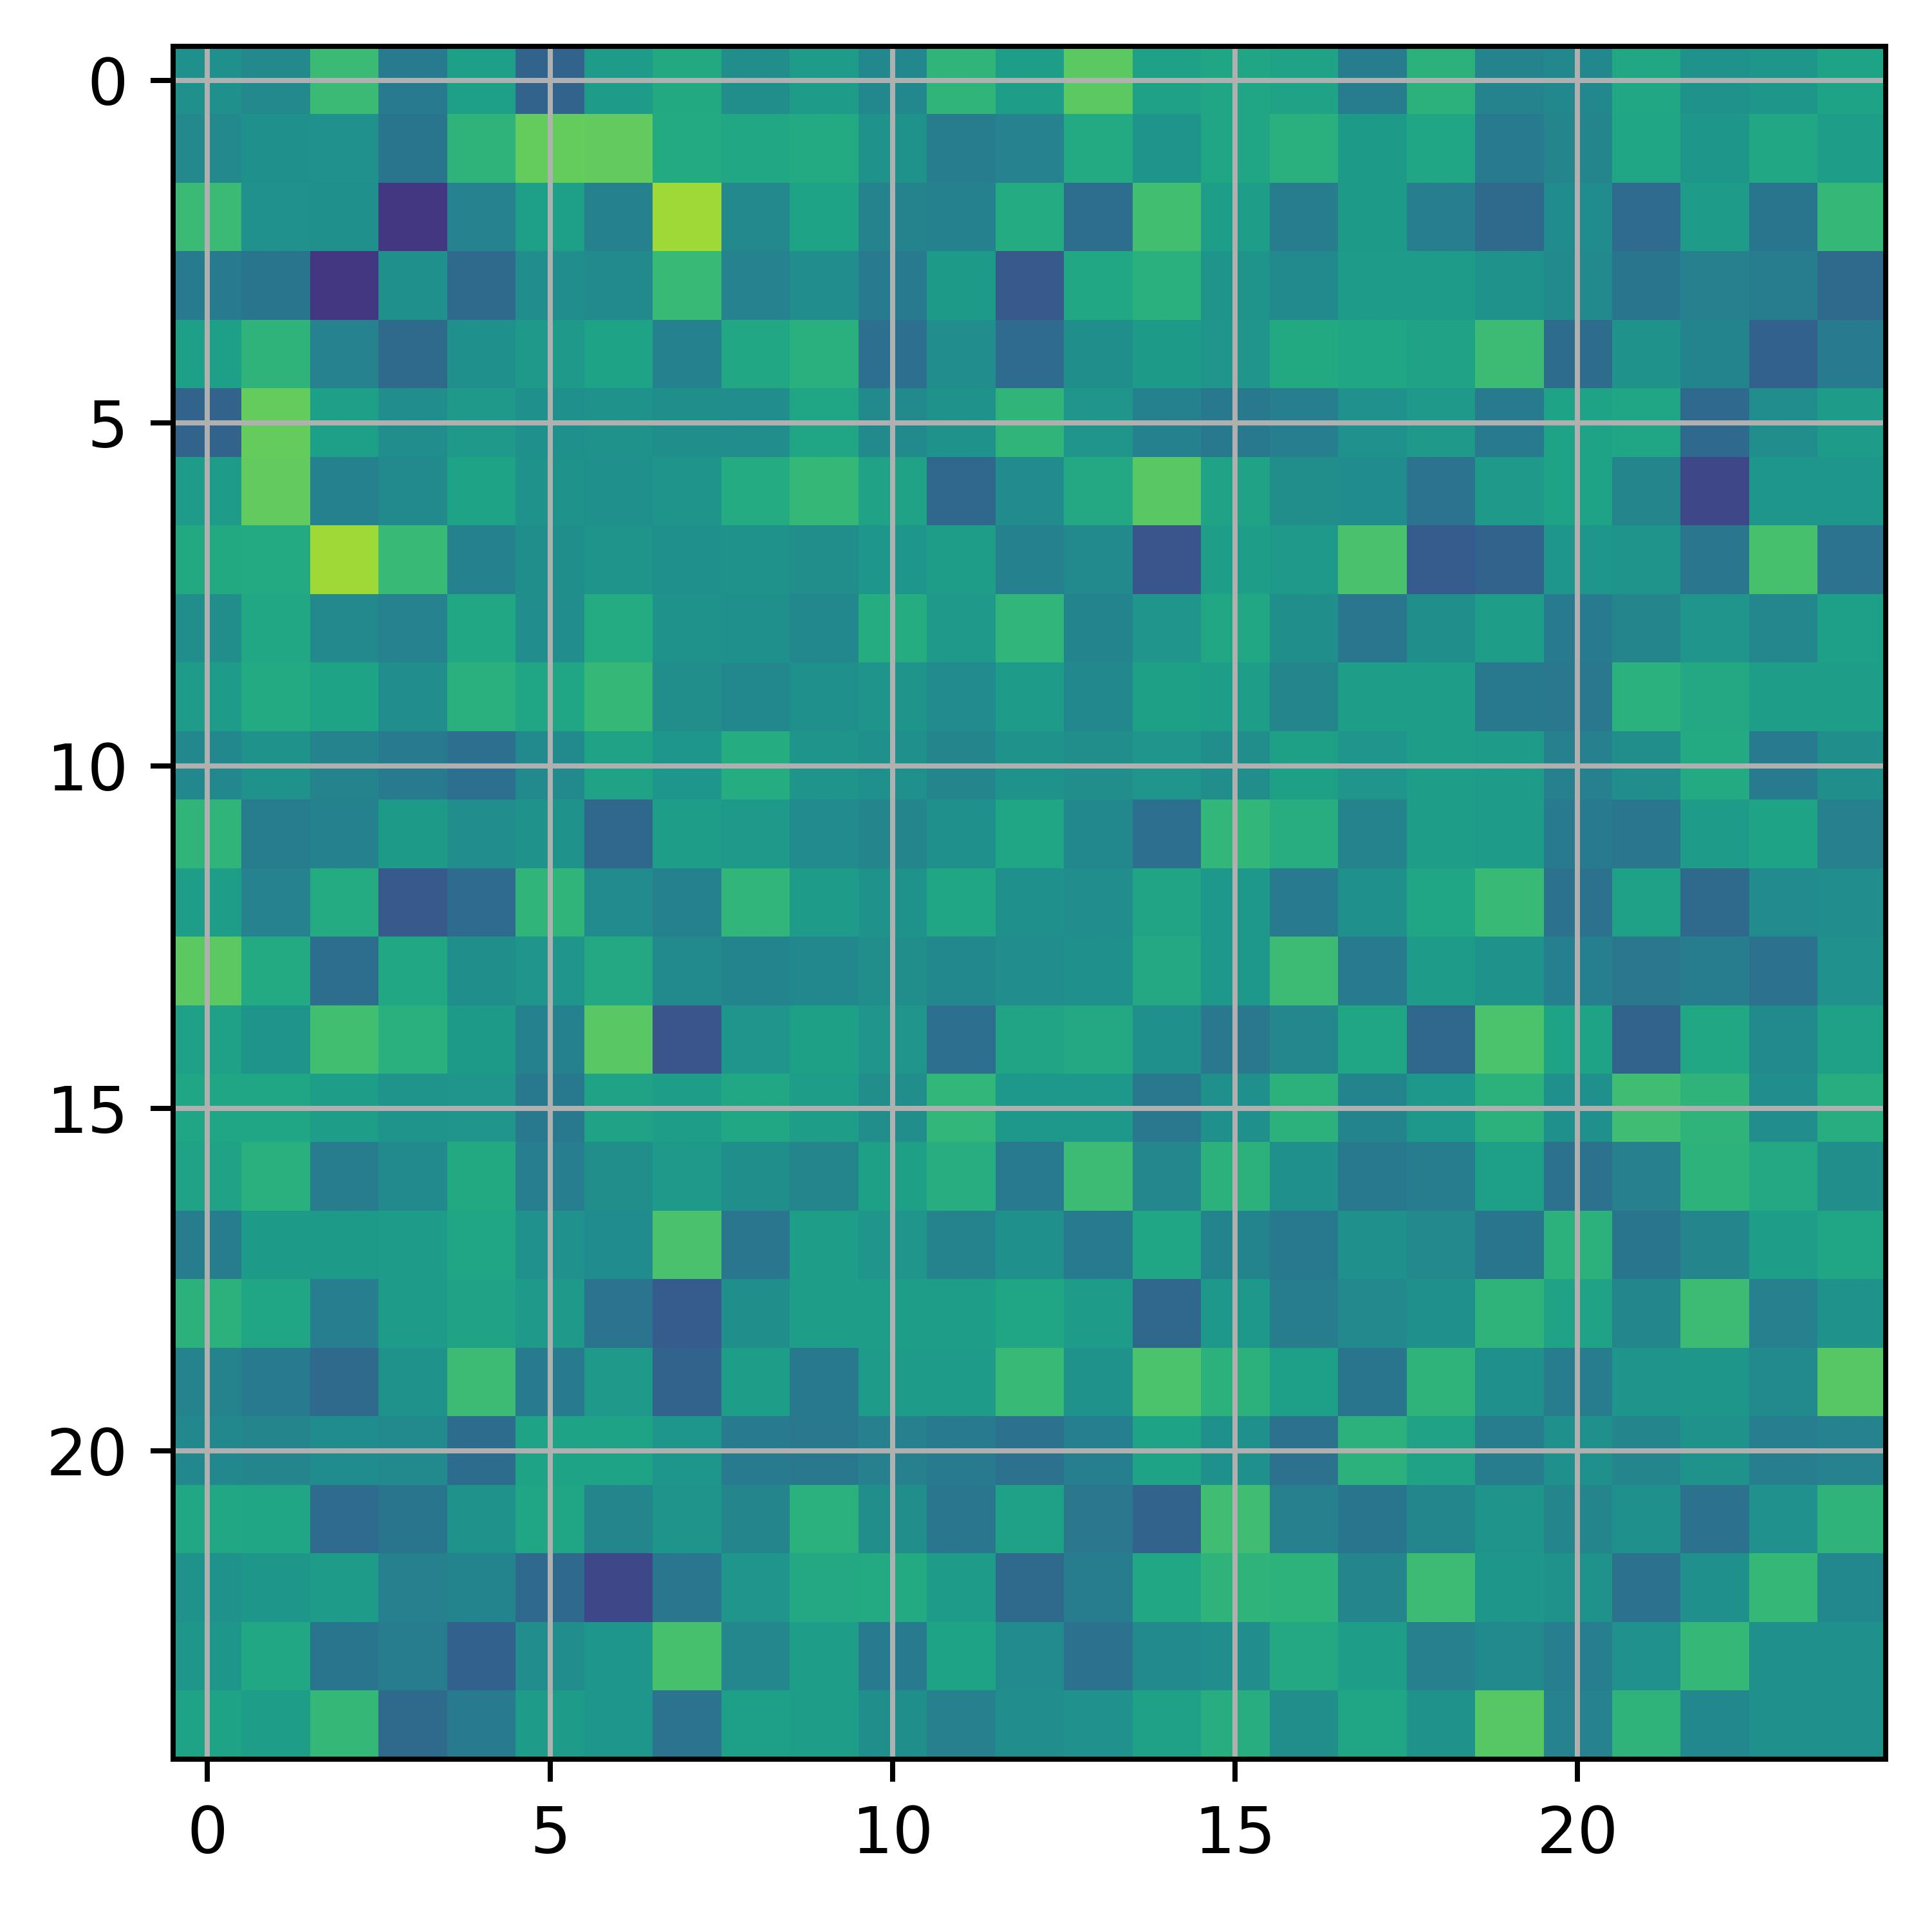
\includegraphics[width=0.18\textwidth]{../Analysis/DFC/size=480_step=180_rho=0.1/node=25_id=100206/n_c_18.jpg}
        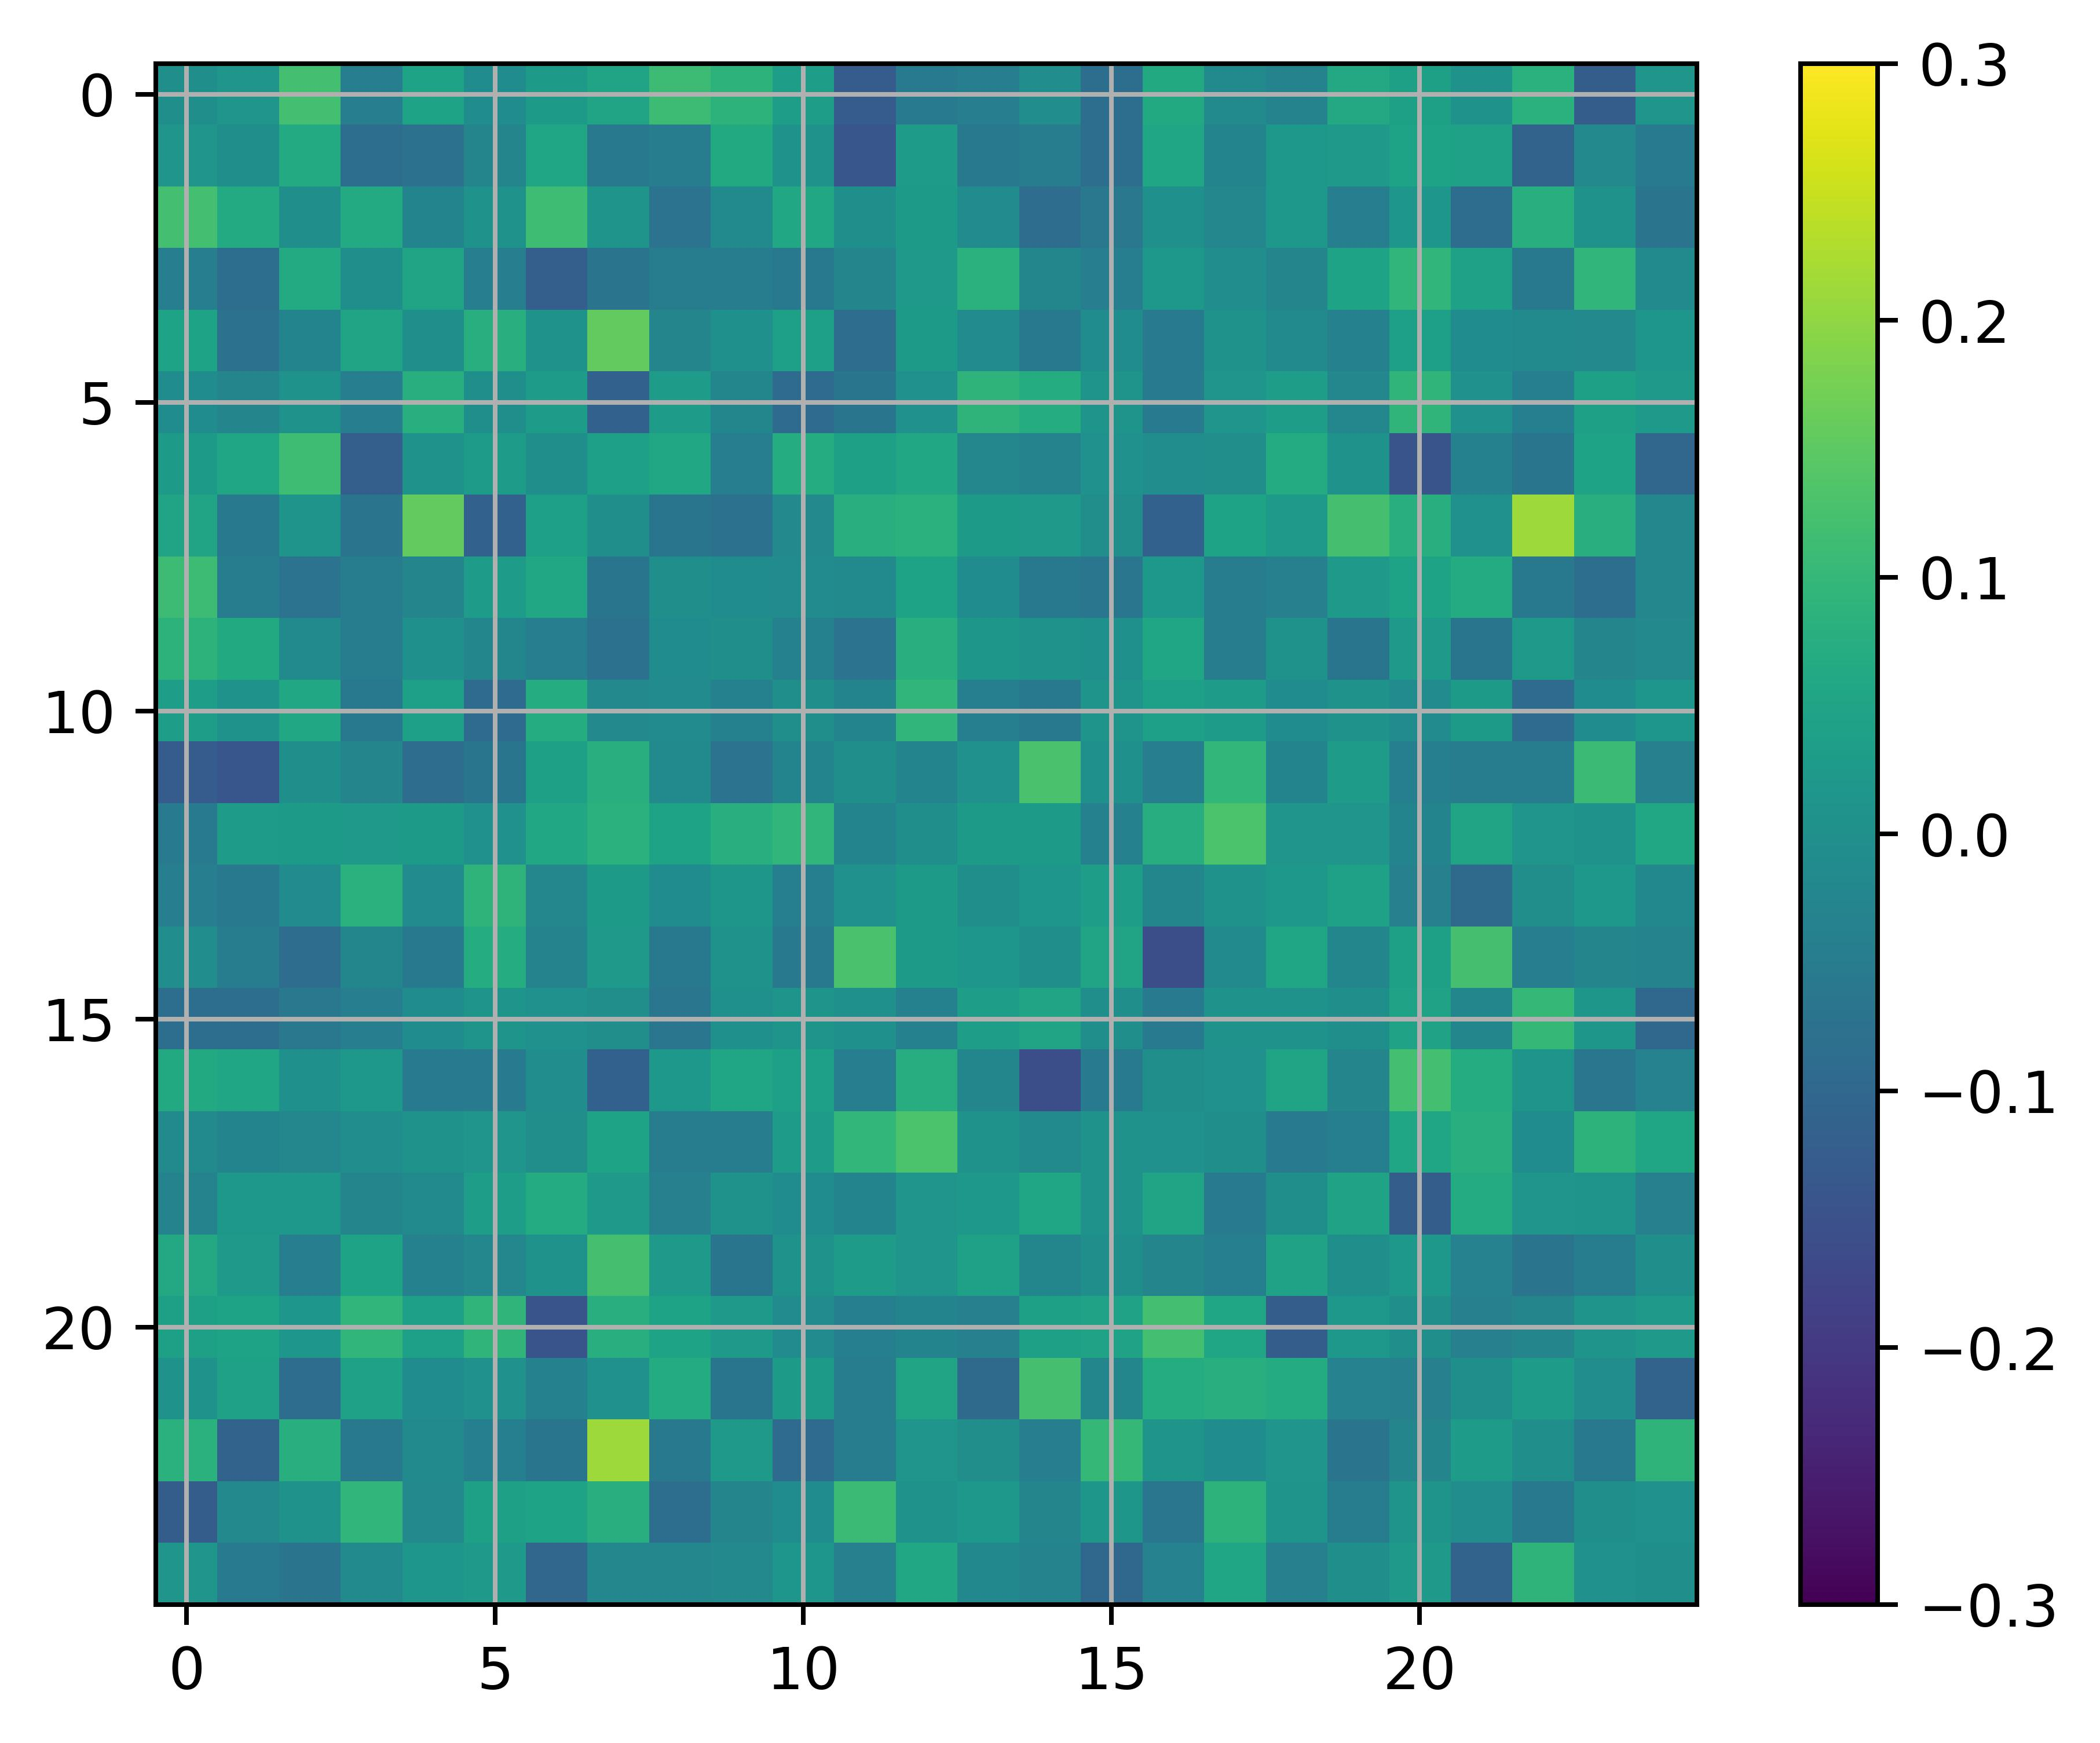
\includegraphics[width=0.2175\textwidth]{../Analysis/DFC/size=480_step=180_rho=0.1/node=25_id=100206/c_24.jpg}} \\
    \subfloat[$N_{\text{node}} = 50$]{
        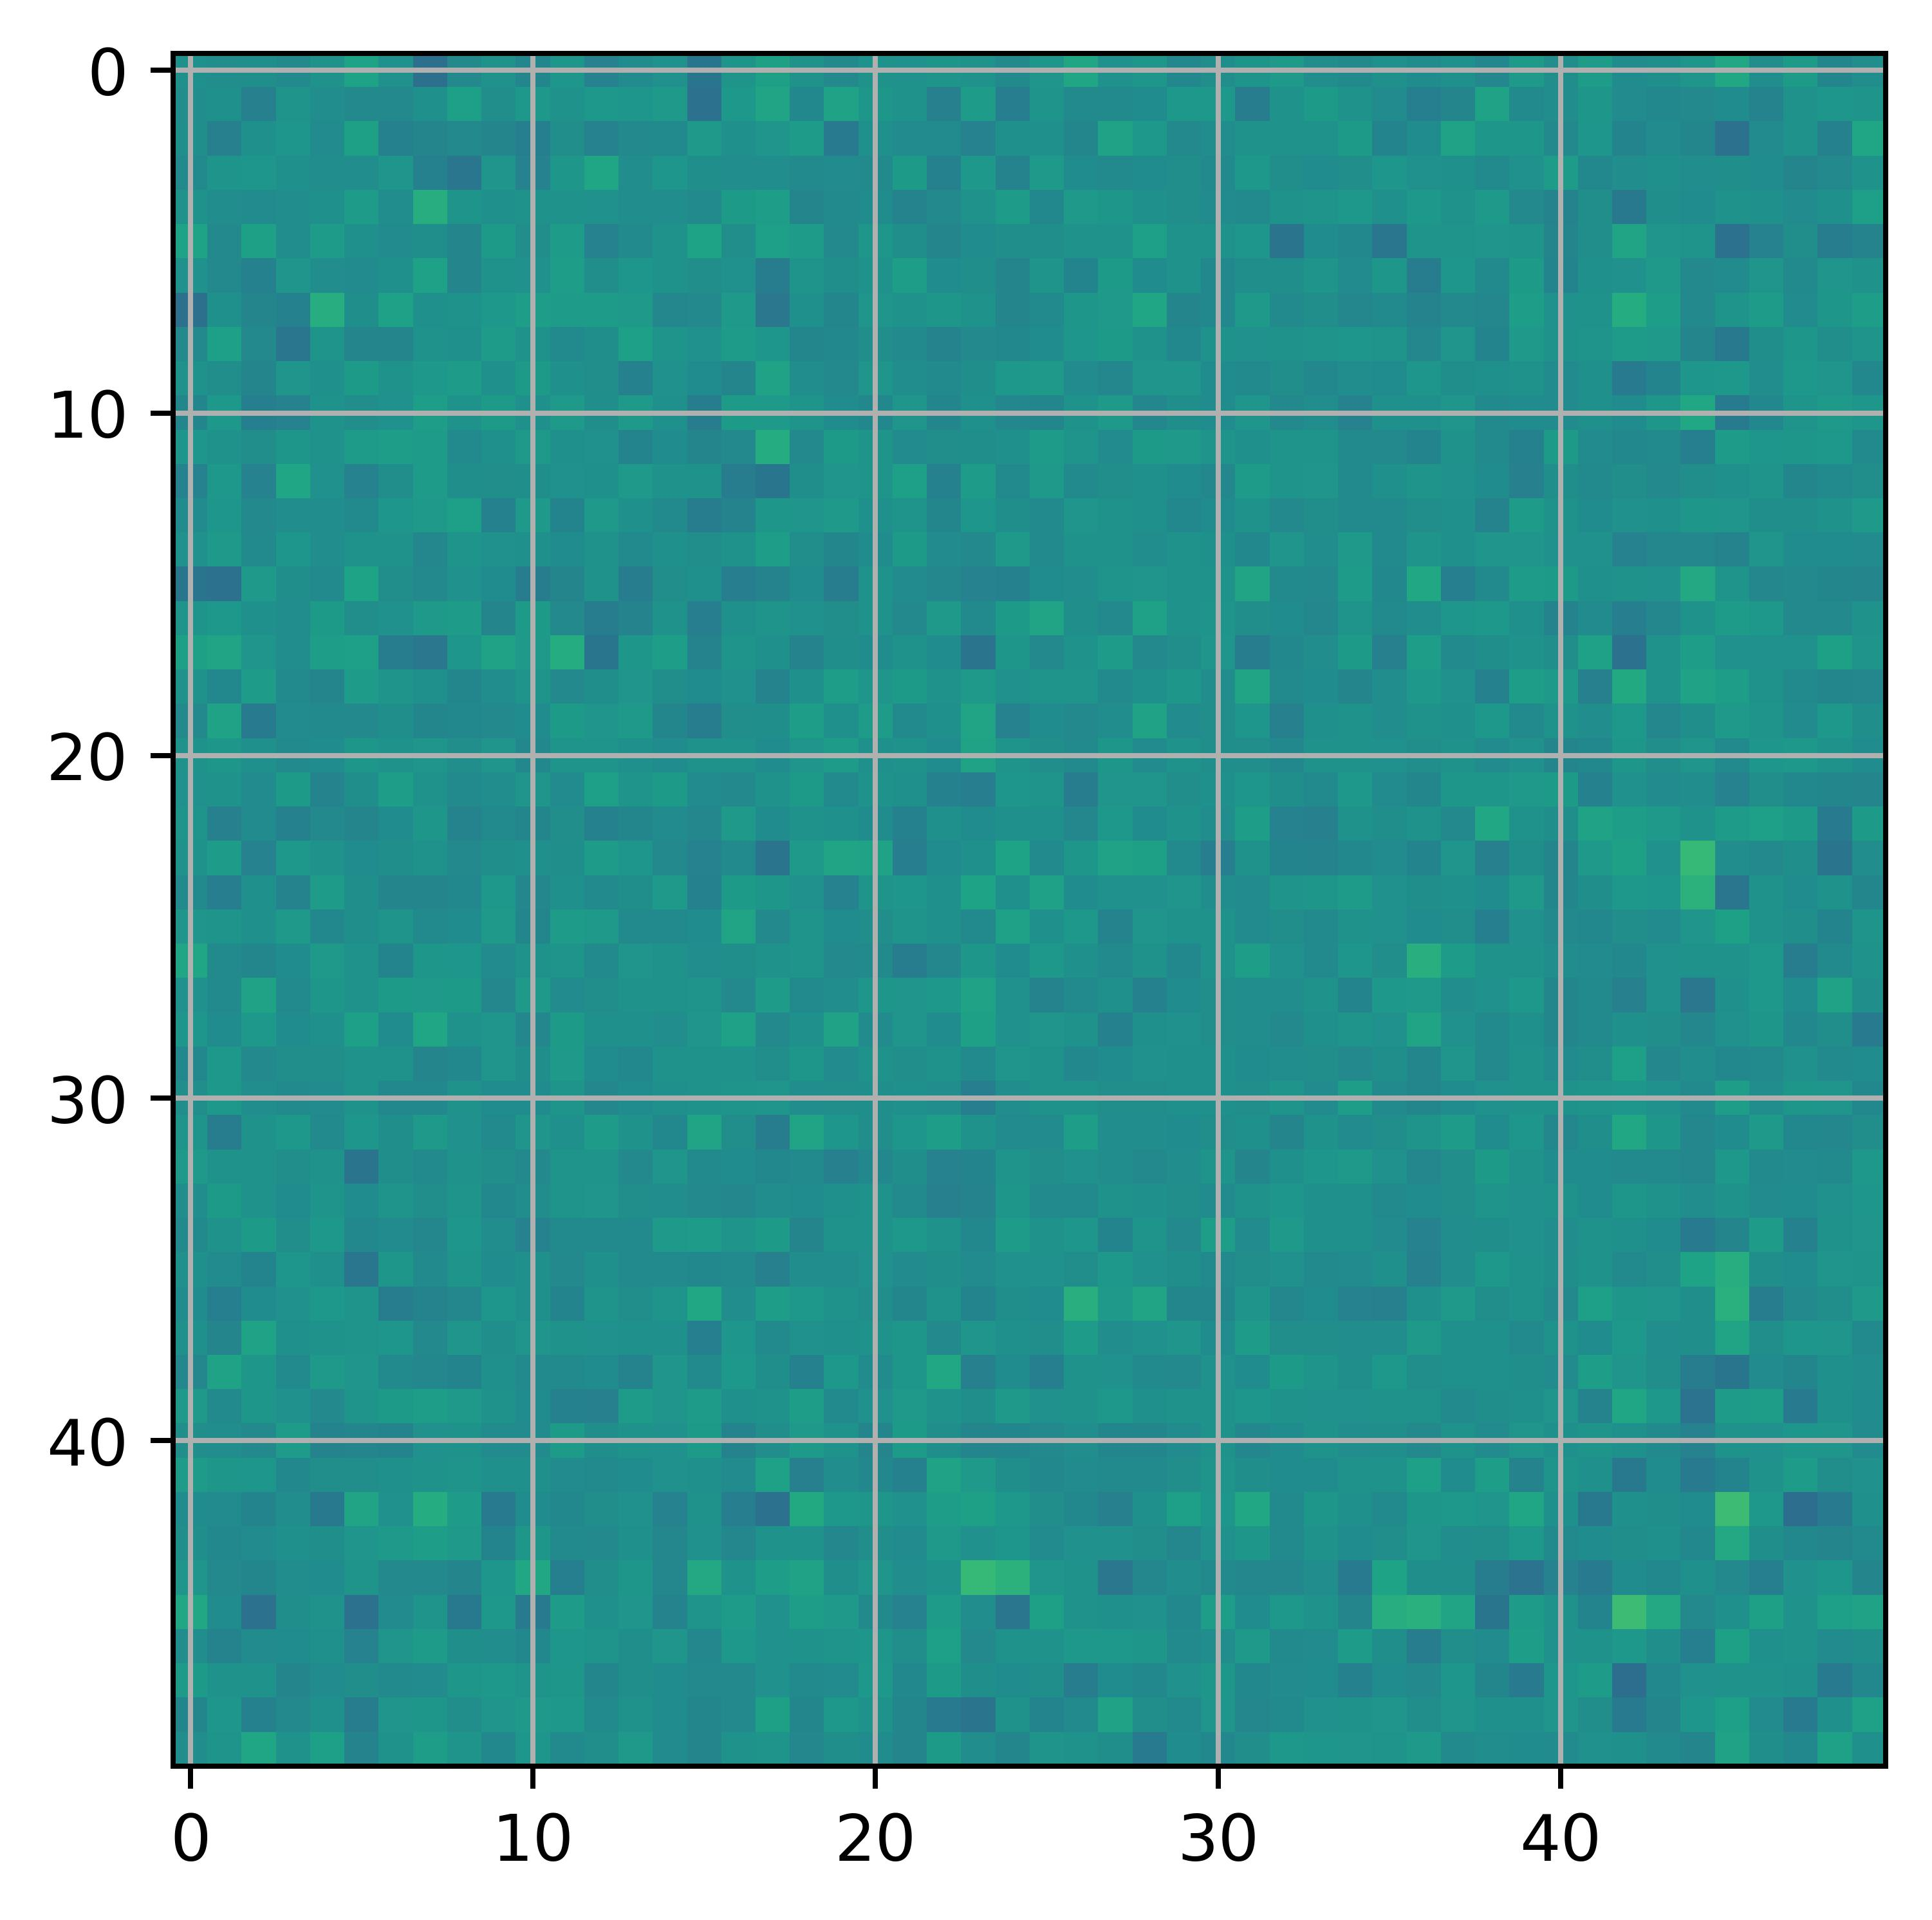
\includegraphics[width=0.18\textwidth]{../Analysis/DFC/size=480_step=180_rho=0.1/node=50_id=100206/n_c_0.jpg}
        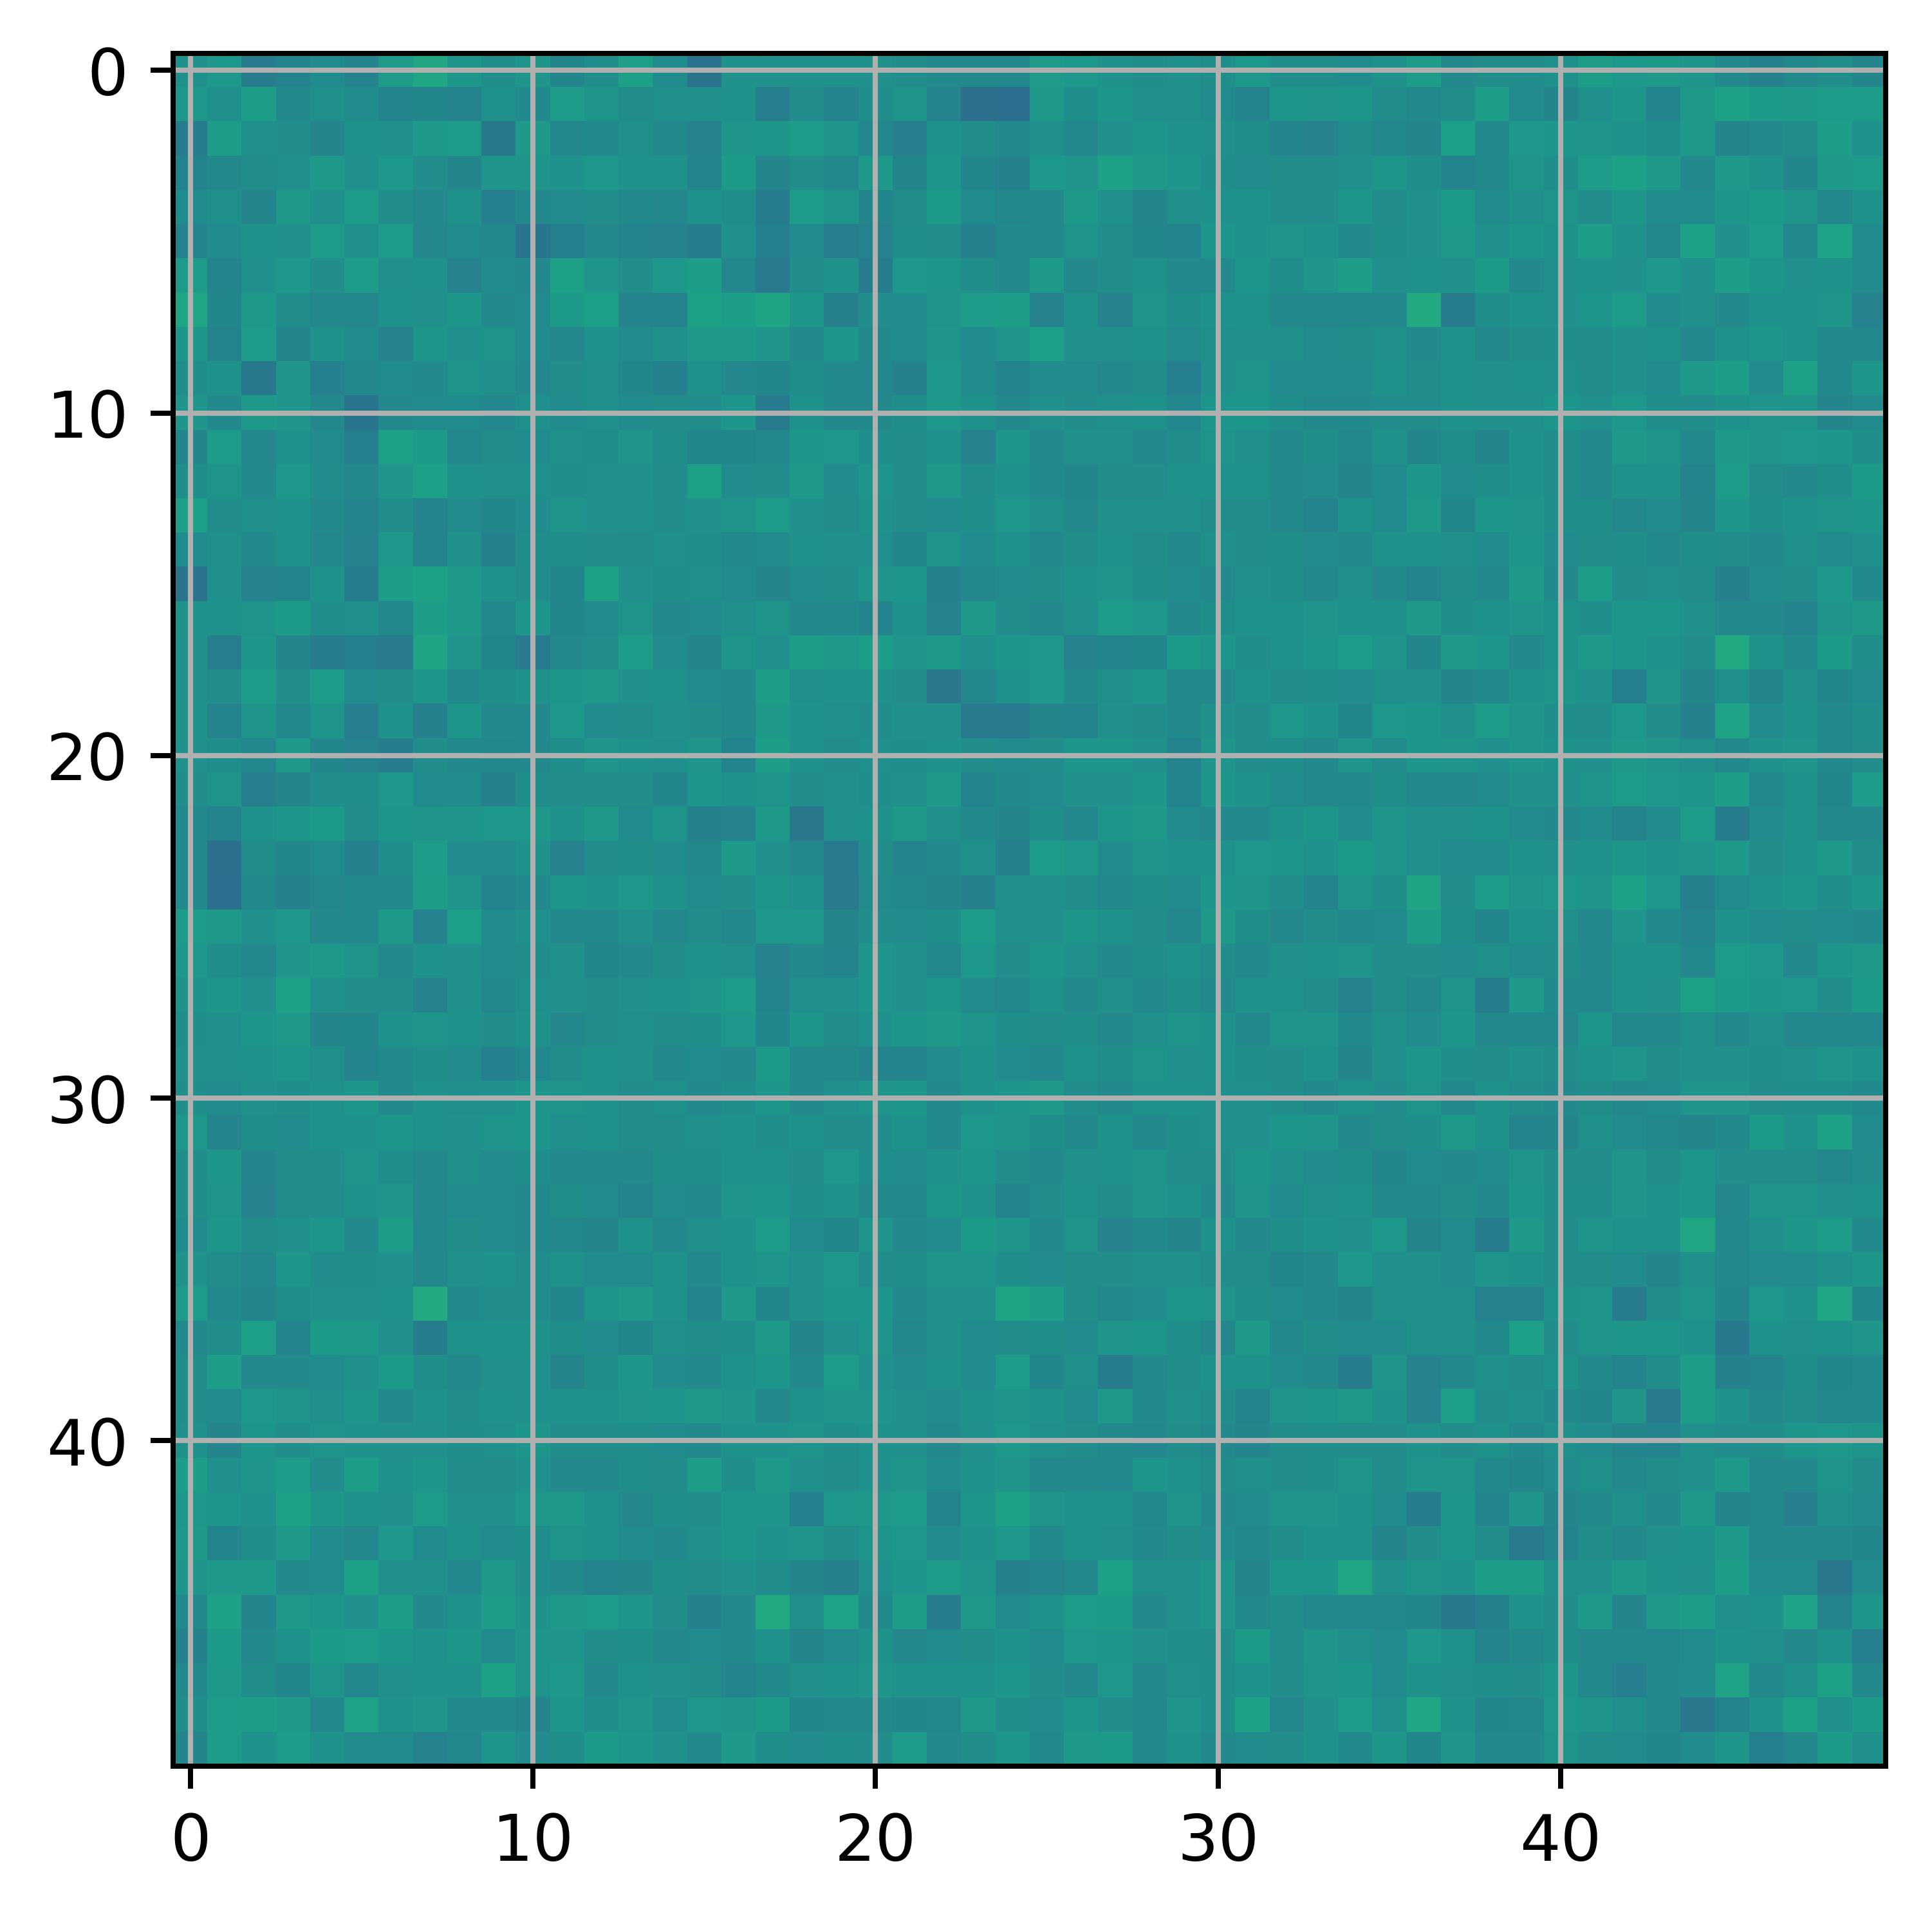
\includegraphics[width=0.18\textwidth]{../Analysis/DFC/size=480_step=180_rho=0.1/node=50_id=100206/n_c_6.jpg}
        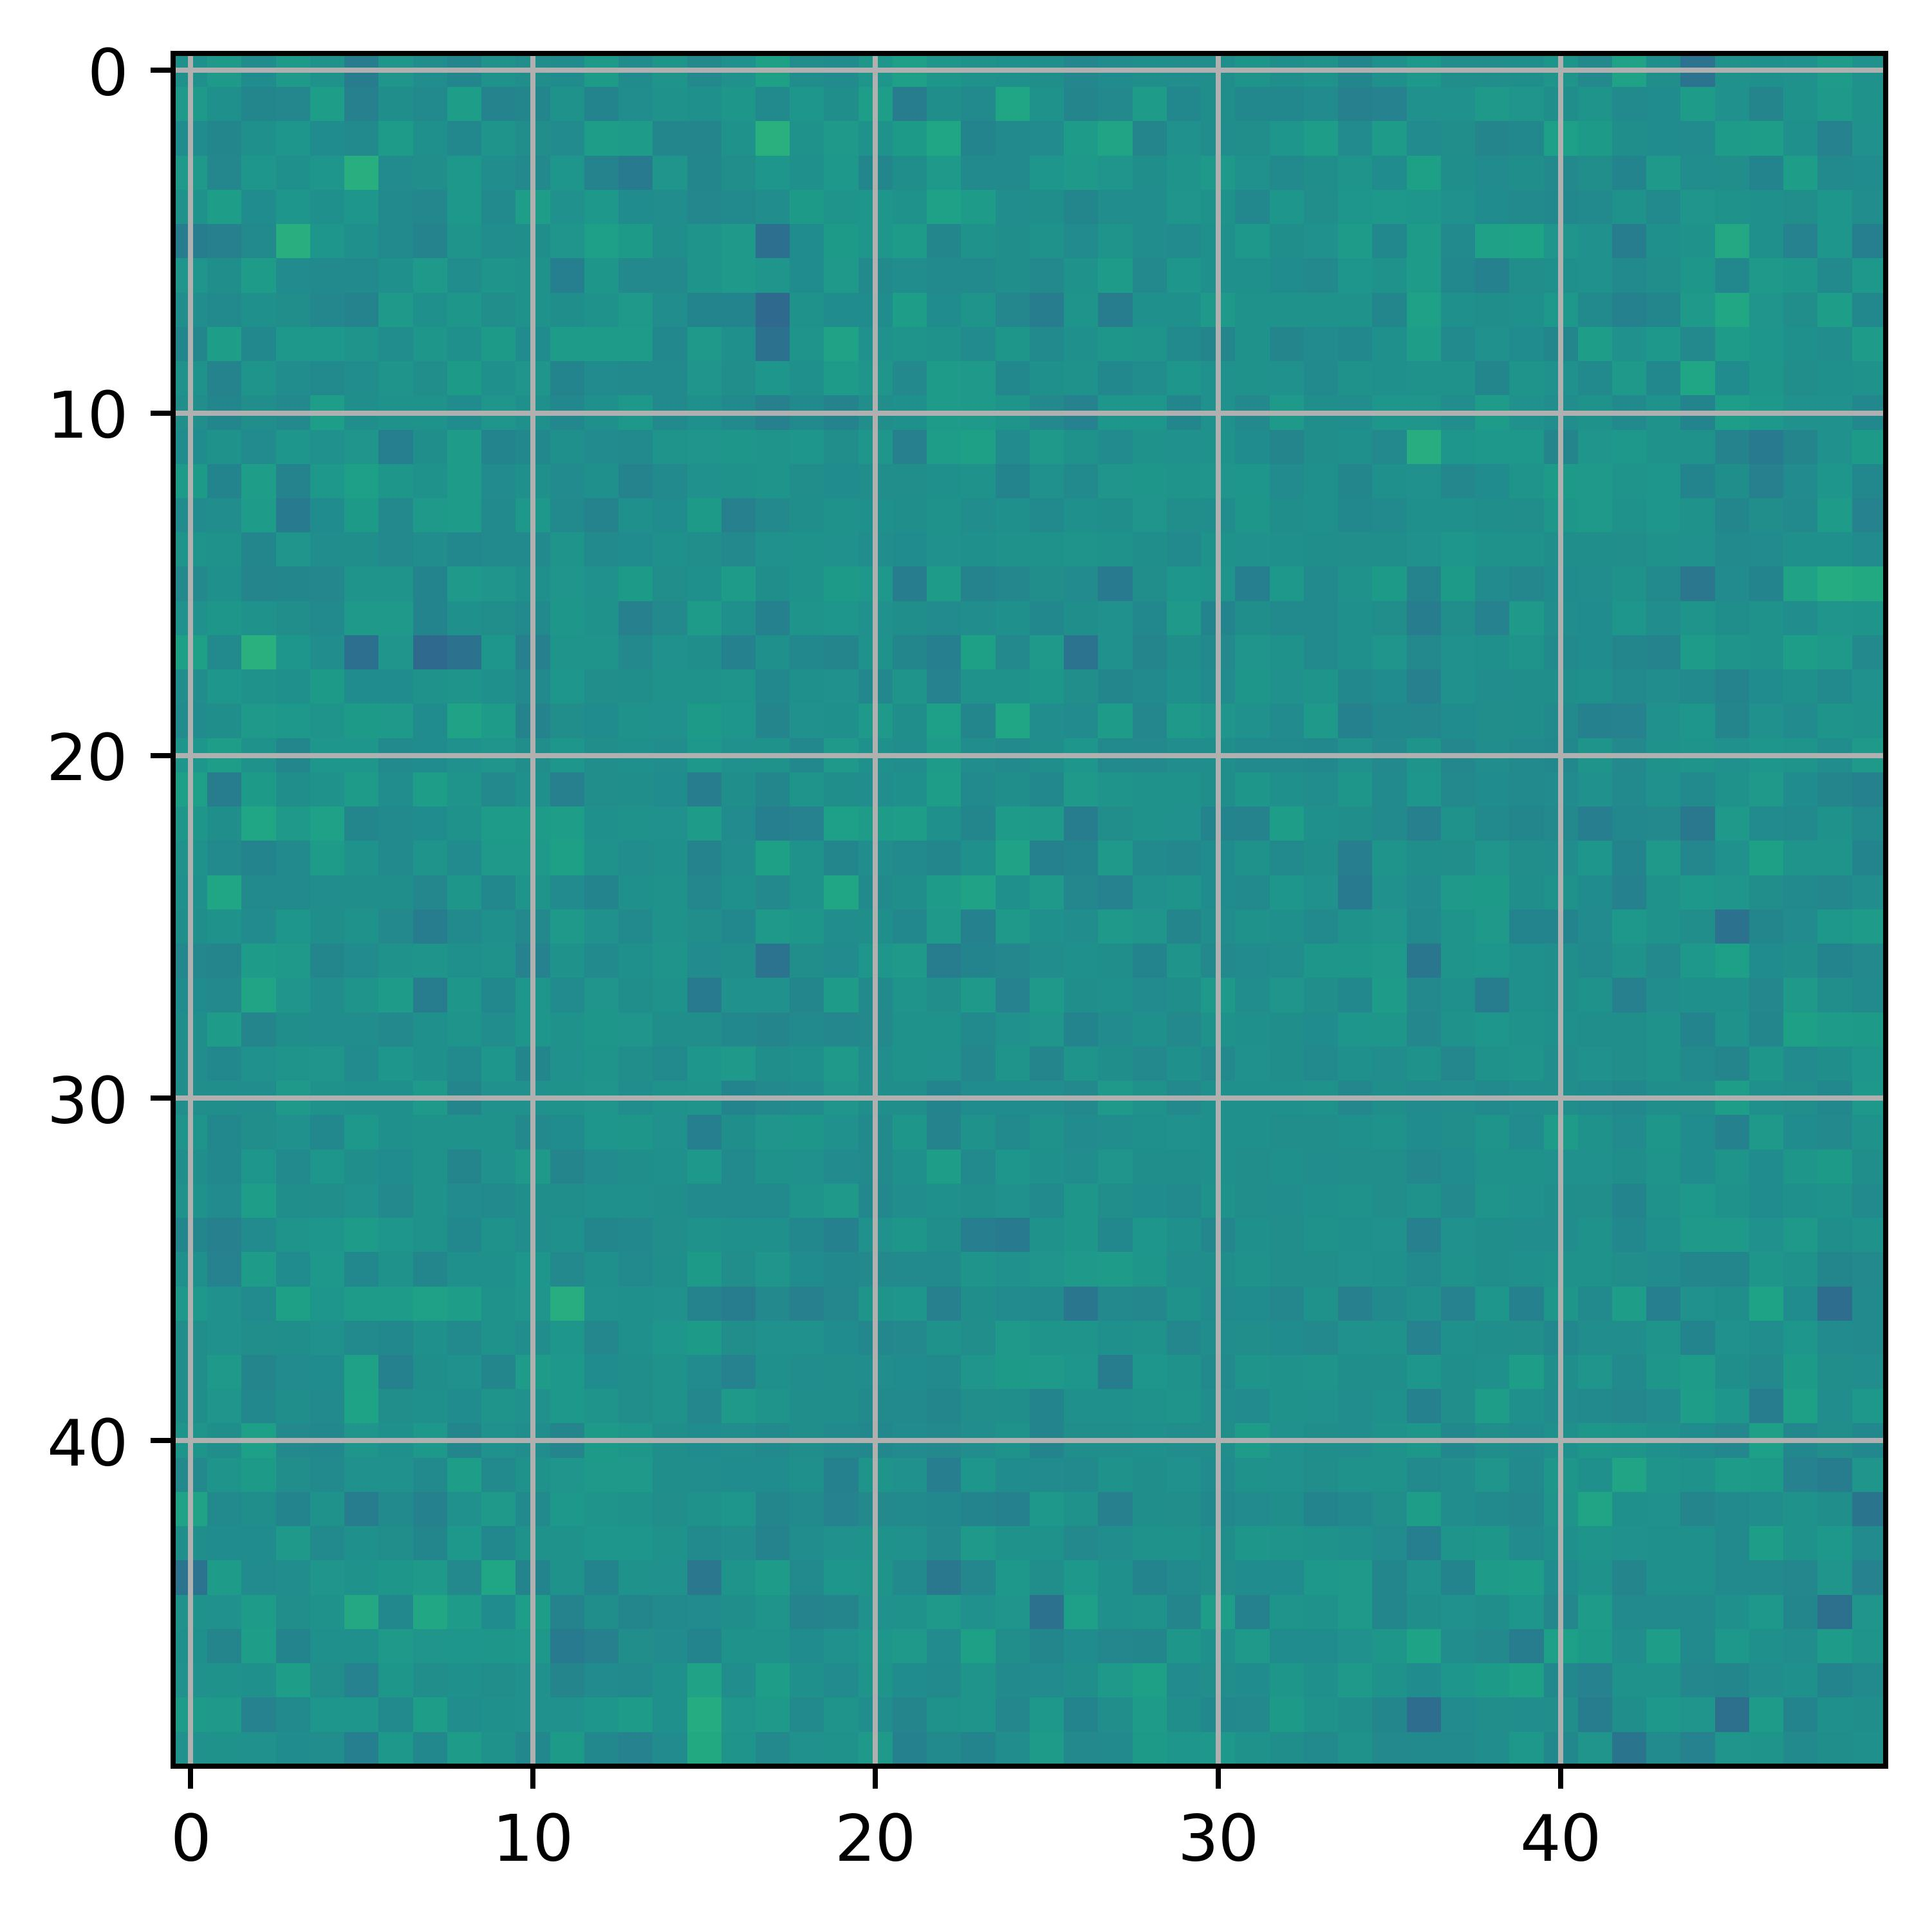
\includegraphics[width=0.18\textwidth]{../Analysis/DFC/size=480_step=180_rho=0.1/node=50_id=100206/n_c_12.jpg}
        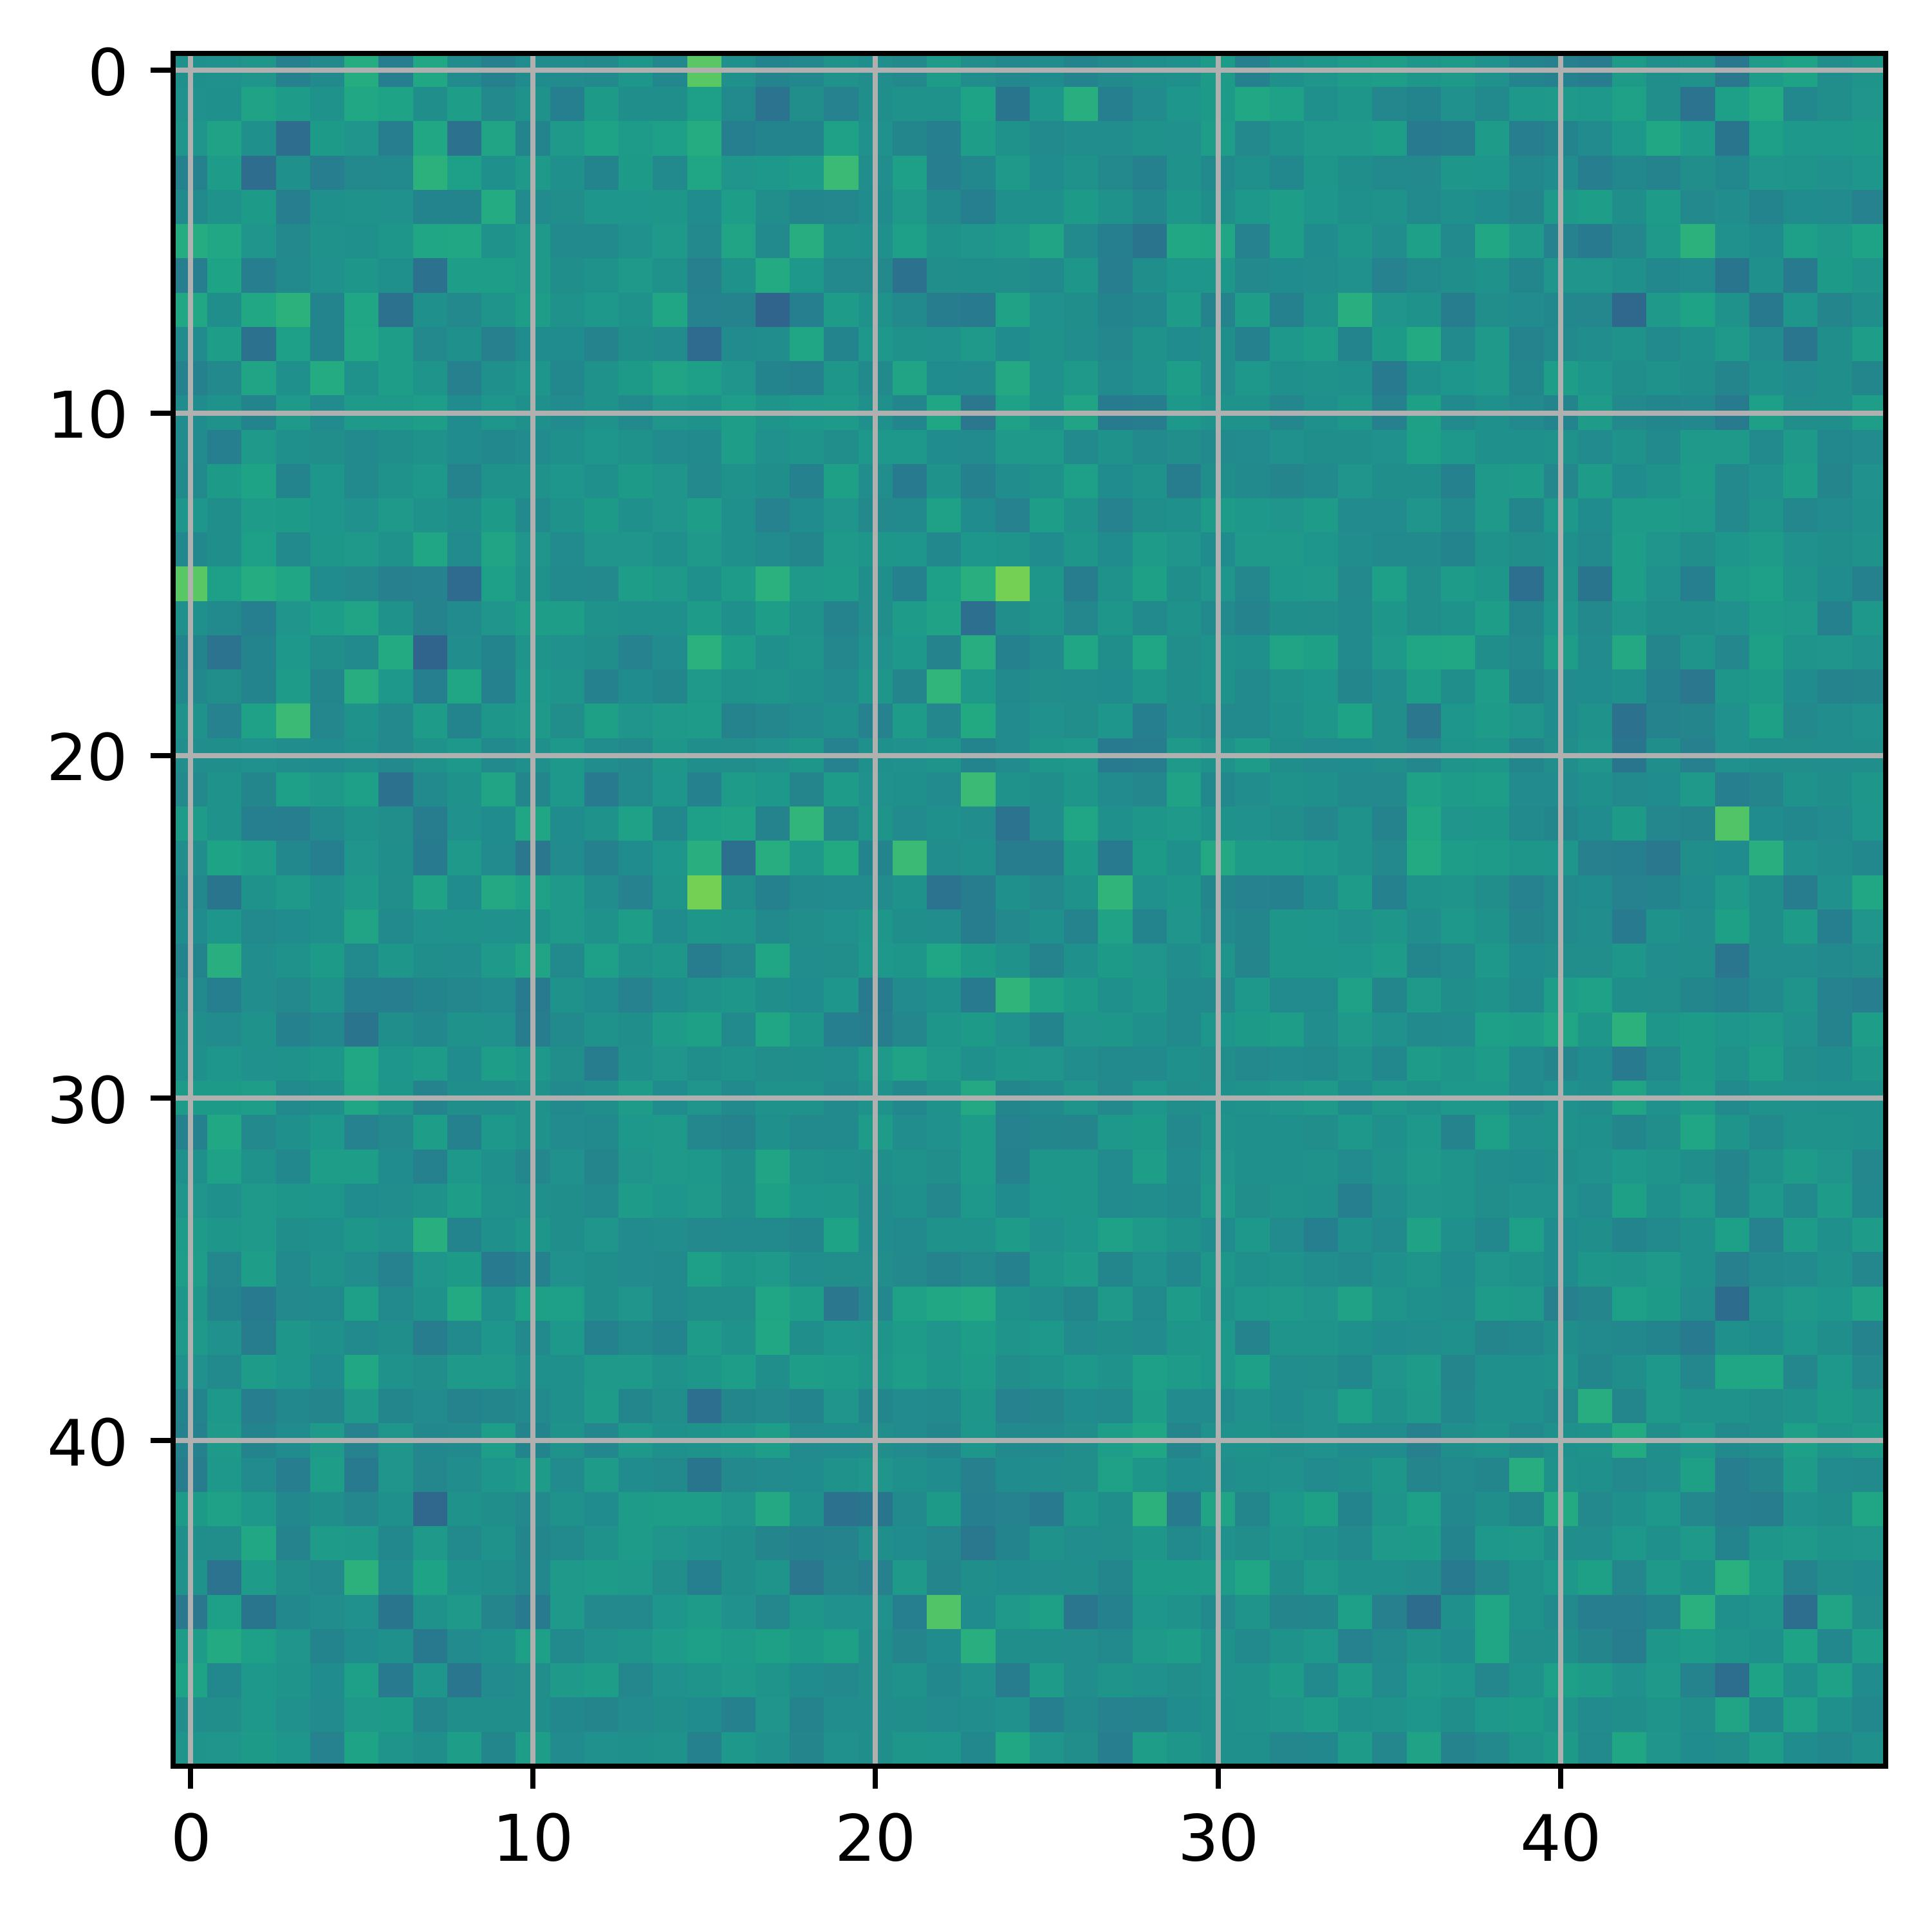
\includegraphics[width=0.18\textwidth]{../Analysis/DFC/size=480_step=180_rho=0.1/node=50_id=100206/n_c_18.jpg}
        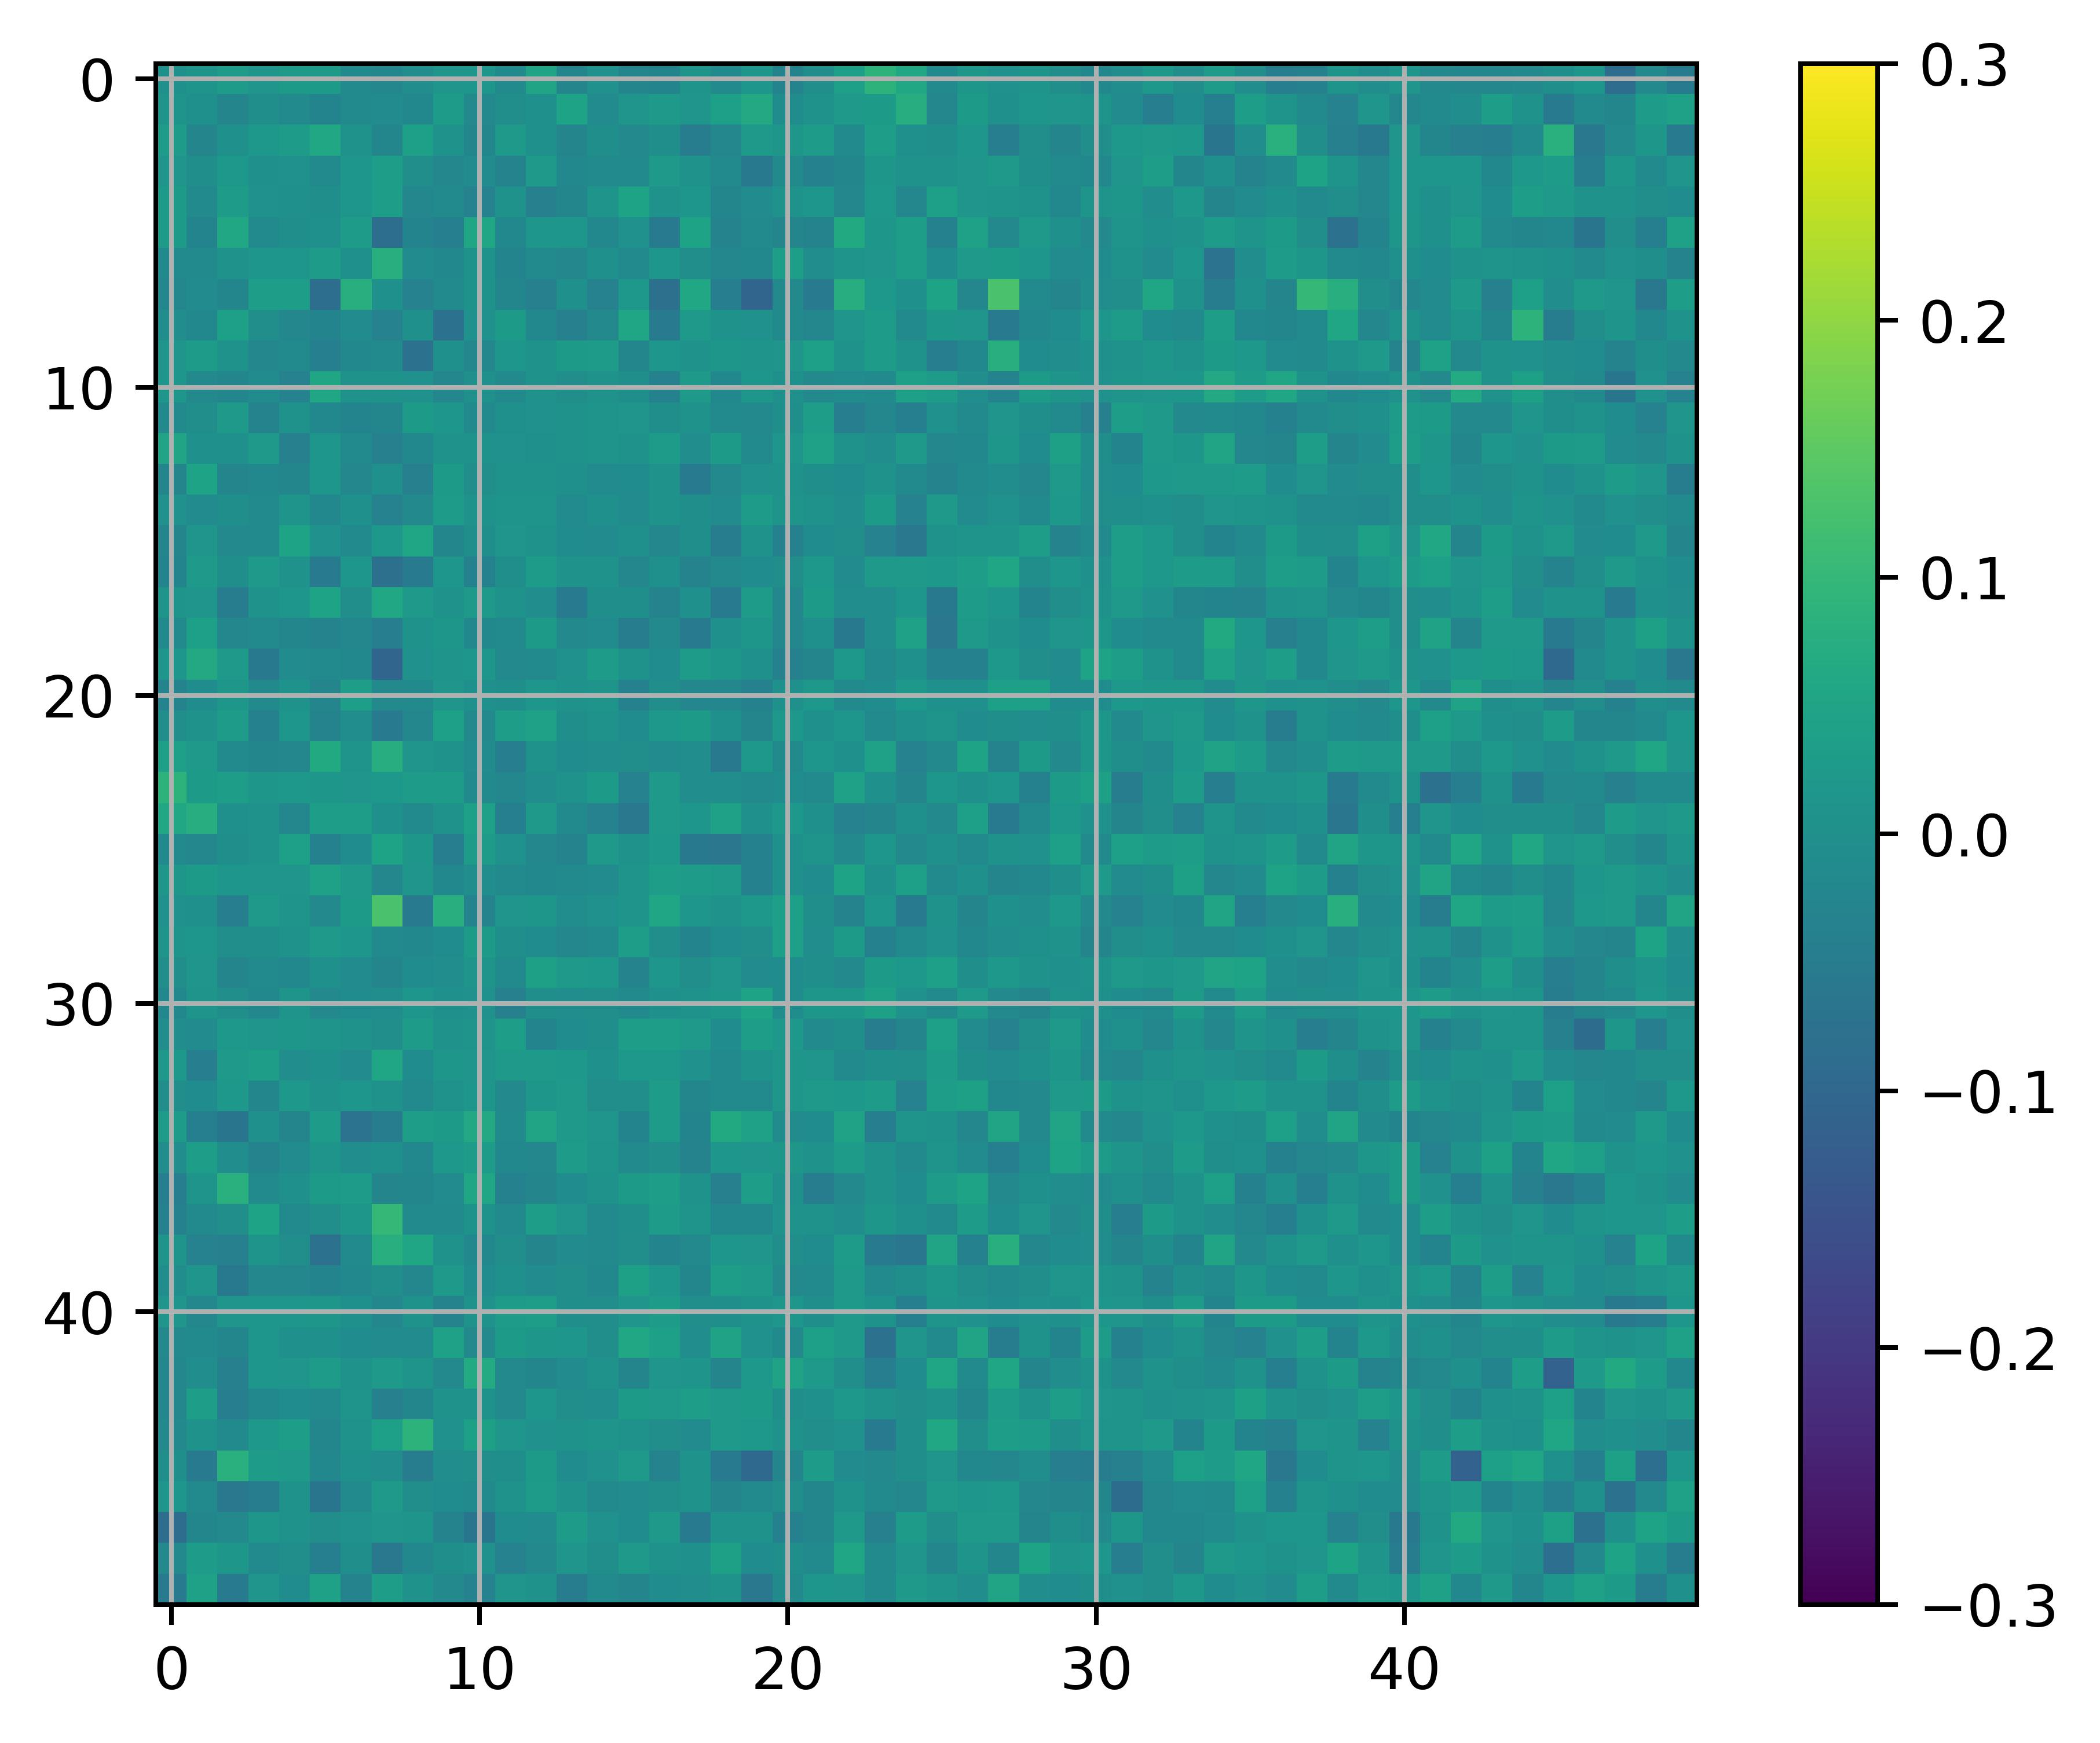
\includegraphics[width=0.2175\textwidth]{../Analysis/DFC/size=480_step=180_rho=0.1/node=50_id=100206/c_24.jpg}}
    \caption{Centered dynamic functional connectivity.}
    \label{sample-dfc-c}
\end{figure}

\begin{table}[H]
    \centering
    \begin{tabular}{|c|c|c|c|}
        \hline
        $N_{\text{node}}$ & min     & mean    & max     \\
        \hline
        $15$              & 5.76e-6 & 2.80e-5 & 1.99e-4 \\
        \hline
        $25$              & 2.82e-6 & 1.07e-5 & 6.07e-5 \\
        \hline
        $50$              & 1.63e-8 & 1.34e-6 & 4.90e-6 \\
        \hline
    \end{tabular}
    \caption{Variance of dFC}
    \label{var-dfc}
\end{table}

\subsection{SVM model}

\subsubsection{Methods}

SVM model \cite{Vapnik1997-yy}\cite{Cortes1995-dg} is a supervised learning algorithm for classification and regression analysis, the core idea of which is to find an optimal hyperplane in the feature space to maximize the spacing between different classes. So we want to find the most suitable hyperplane to divide the genders.
Since it is hard to determine whether the brain network data is linearly separable before conducting experiments about SVM, we use both the linear SVM and the NuSVM model to train the brain network data respectively.

\subsubsection{Results and Conclusions}

The experimental results for SVM show that the classification accuracy of the model rises with the increase of nodes of the data. Taking the maximum AUC in different nodes as examples, it is 87.56\% for 15-node data, 92.02\% for 25-node data, and 97.49\% for 50-node data. These numerical results indicate that when the regional features are convergent, the classification accuracy will be correspondingly improved. Additionally, among all tests, the dynamic data of 15 nodes demonstrates the lowest accuracy, which is approximately at 69\%. This indicates that both dynamic and static functional connectivity data are linearly separable.

However, when comparing the classification accuracy of dynamic data and static data under the same nodes, the performance of dynamic data is not better than that of static data. This might be attributed to some complex features that dynamic data takes so that it is difficult to extract all of them efficiently using single hyperplane. Therefore, we consider to train brain network data by CNN with `multiple hyperplanes'.

\begin{figure}[H]
    \centering
    \subfloat[Linear SVM]{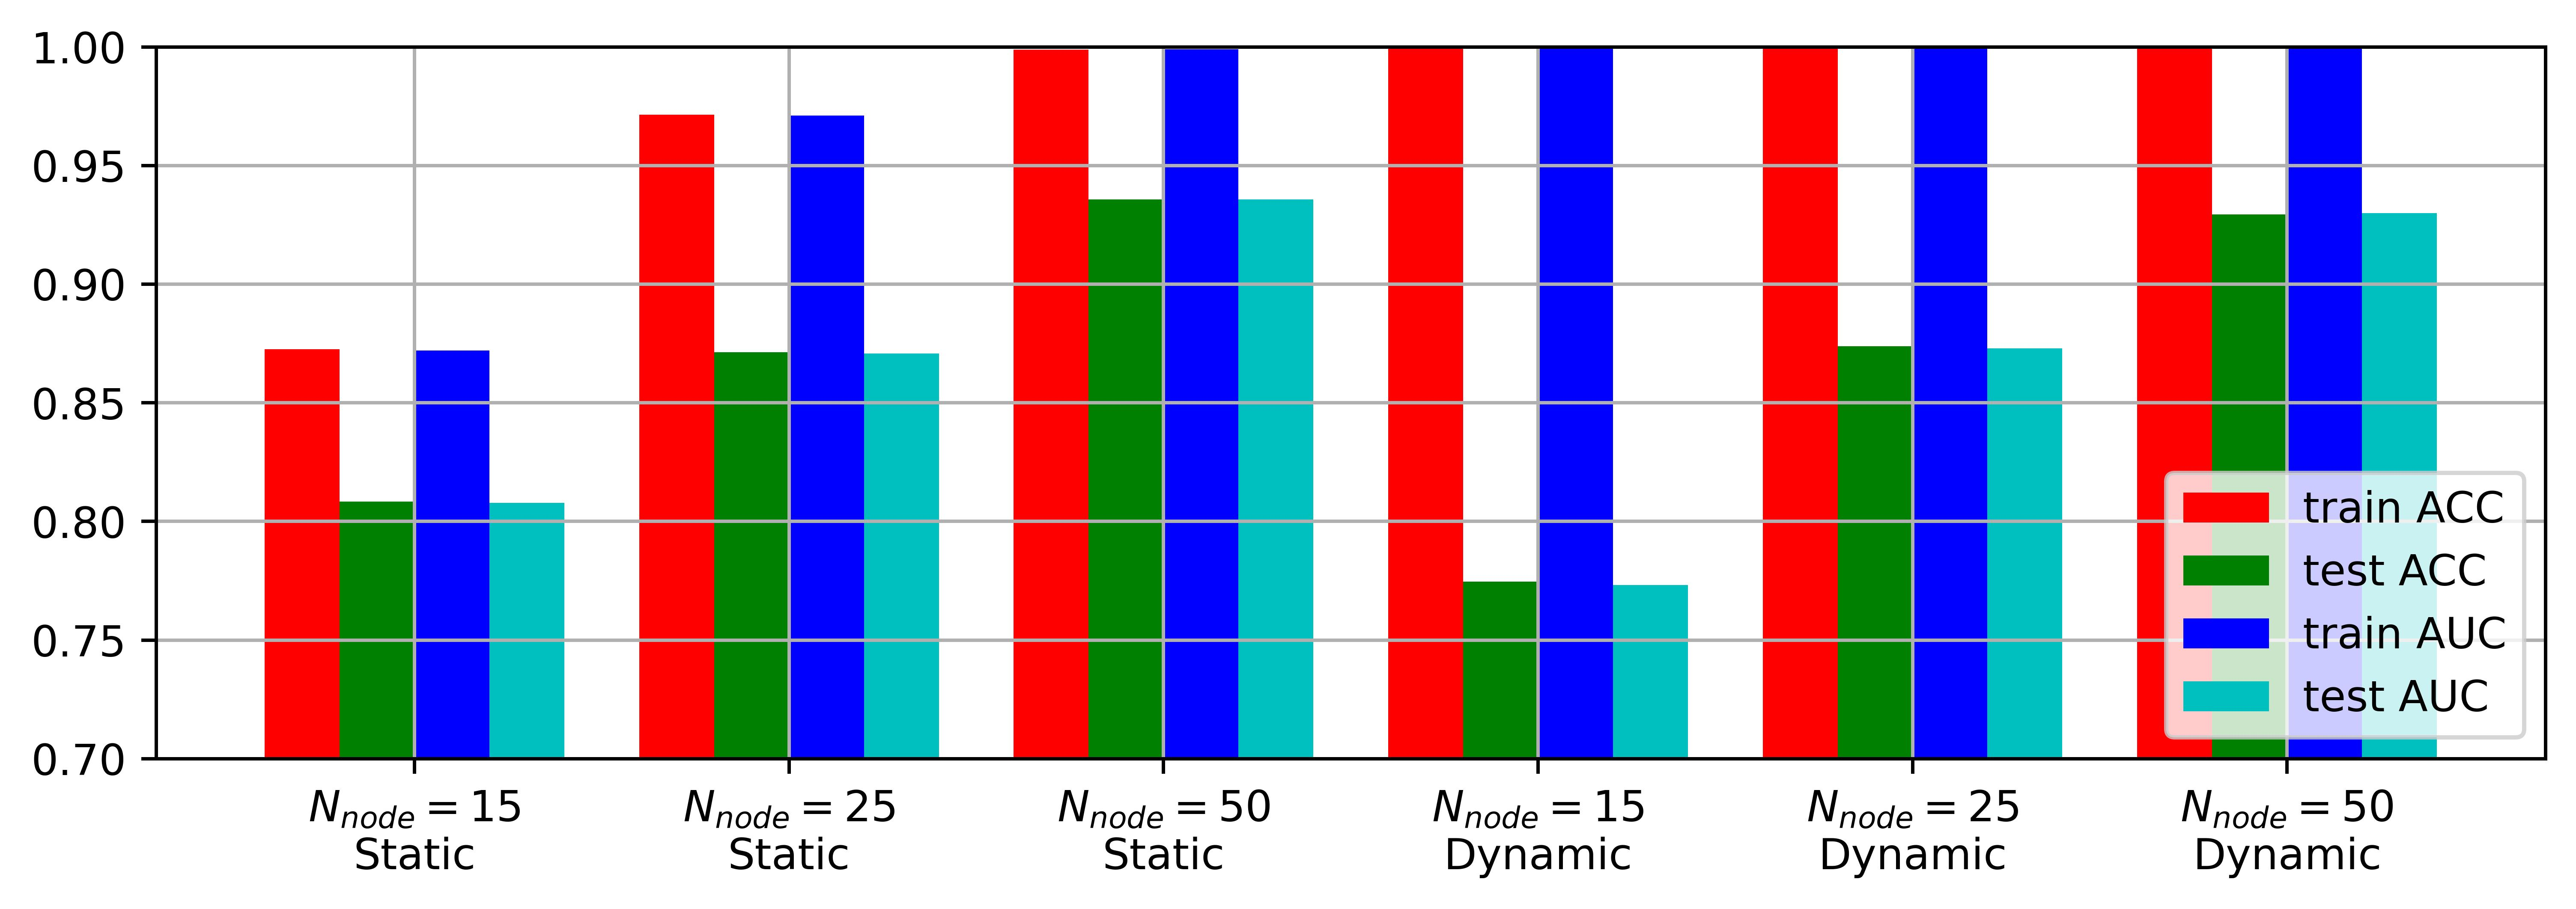
\includegraphics[width=0.5\textwidth]{../SVM/linear_0.1.jpg}}
    \subfloat[Nu-SVM]{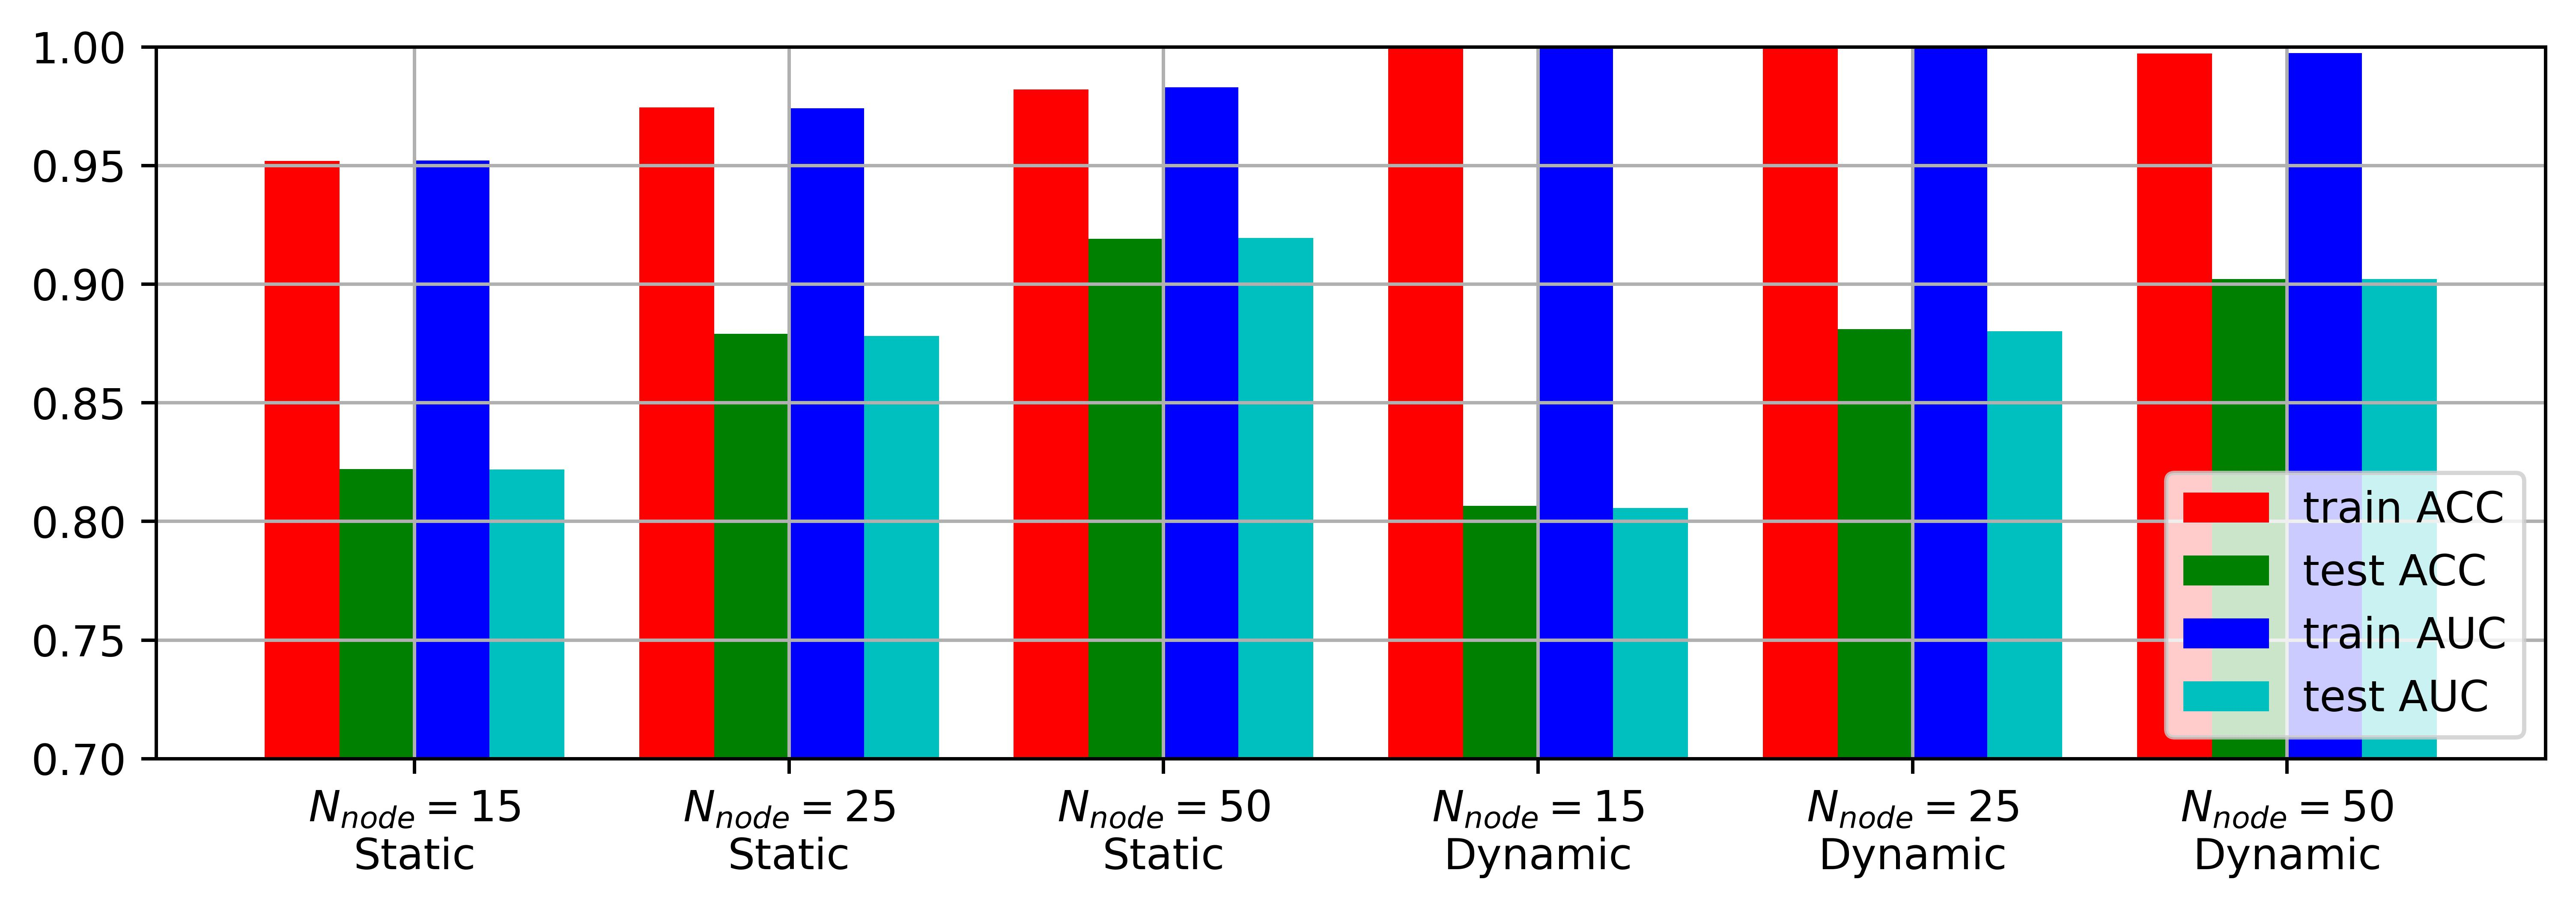
\includegraphics[width=0.5\textwidth]{../SVM/nu_0.1.jpg}}
    \caption{Results of SVM model.}
    \label{svm-results}
\end{figure}

\subsection{CNN model}

\subsubsection{Methods}

Convolutional Neural Networks(CNN) is a class of feedforward neural networks with convolutional computation and deep structures. We choose the CNN model because CNN can automatically learn and extract complex features of data through its multi-layer convolution structure, and each layer can be seen as segmenting the data at different levels of abstraction, which is equivalent to using multiple hyperplanes to divide the data. And in the worst-case scenario, where all hyperplanes are the same, the model is linear SVM, and its results should be the same as SVM.

We use m hyperplanes to divide the preprocessed data, extract m feature vectors and correspond to one-to-one, and then use Multilayer Perceptron(MLP) to divide these features into two categories, male and female. The followings are flowchart of our method, where we use a 1-layer 1-dimensional CNN with size equivalent to the input shape, so that it is the same as previous statements.

\begin{figure}[H]
    \centering
    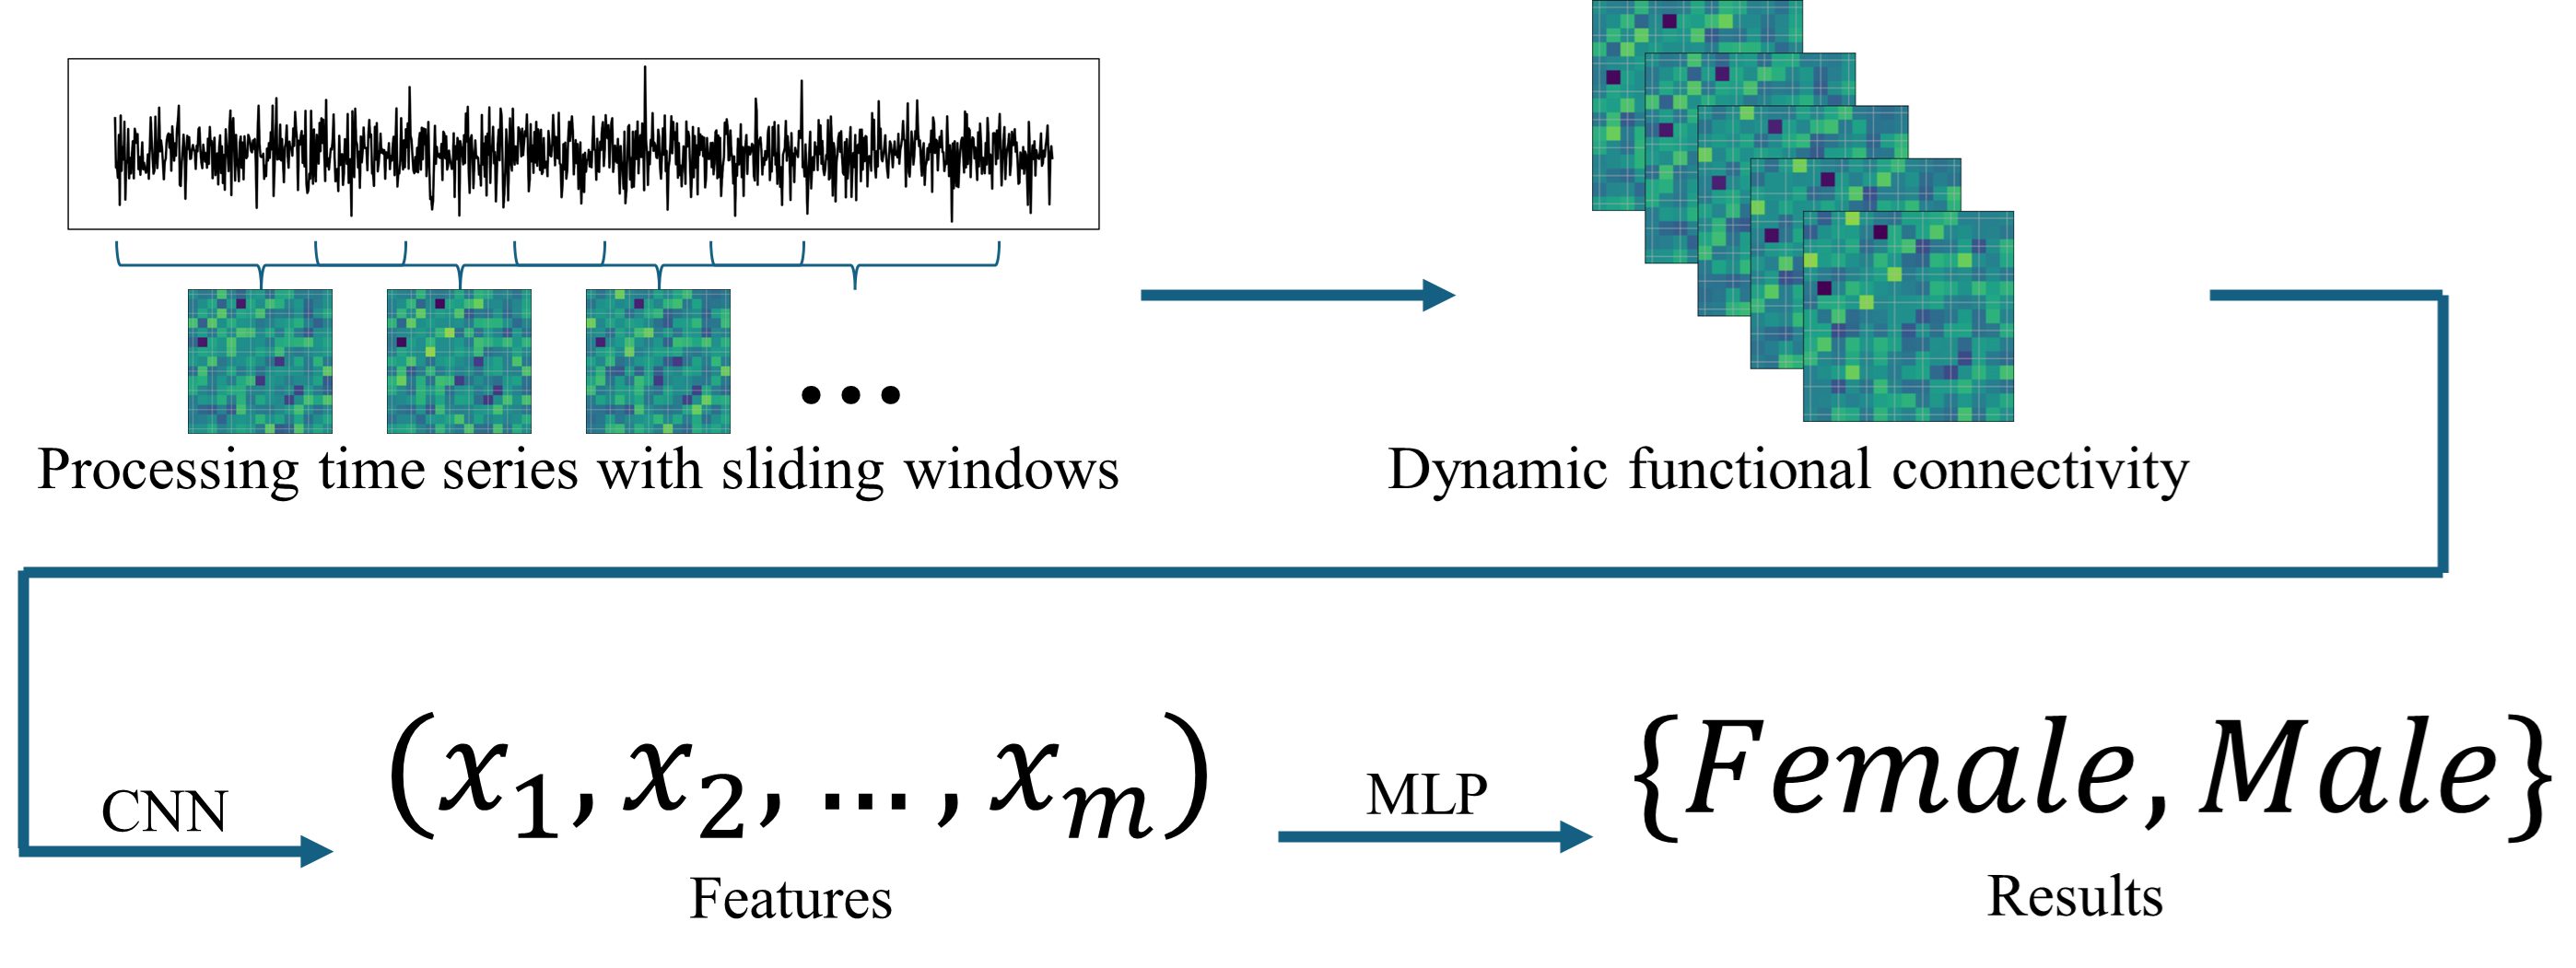
\includegraphics[width=0.8\textwidth]{./figure/method.png}
    \label{figure-CNN-model}
\end{figure}

We split the data into training dataset(80\%) and test dataset(20\%), and repeat the experiment for 150 times to avoid flukes.

\subsection{Results and Conclusions}

Figure \ref{CNN-results} illustrates the overall results of the data training by CNN. The first 6 columns present the classification results using all frame data, while the last 3 columns describe the results with one frame data that randomly selected. It is remarkable that the classification accuracy is significantly lower when using parts of frame data.

\begin{figure}[H]
    \centering
    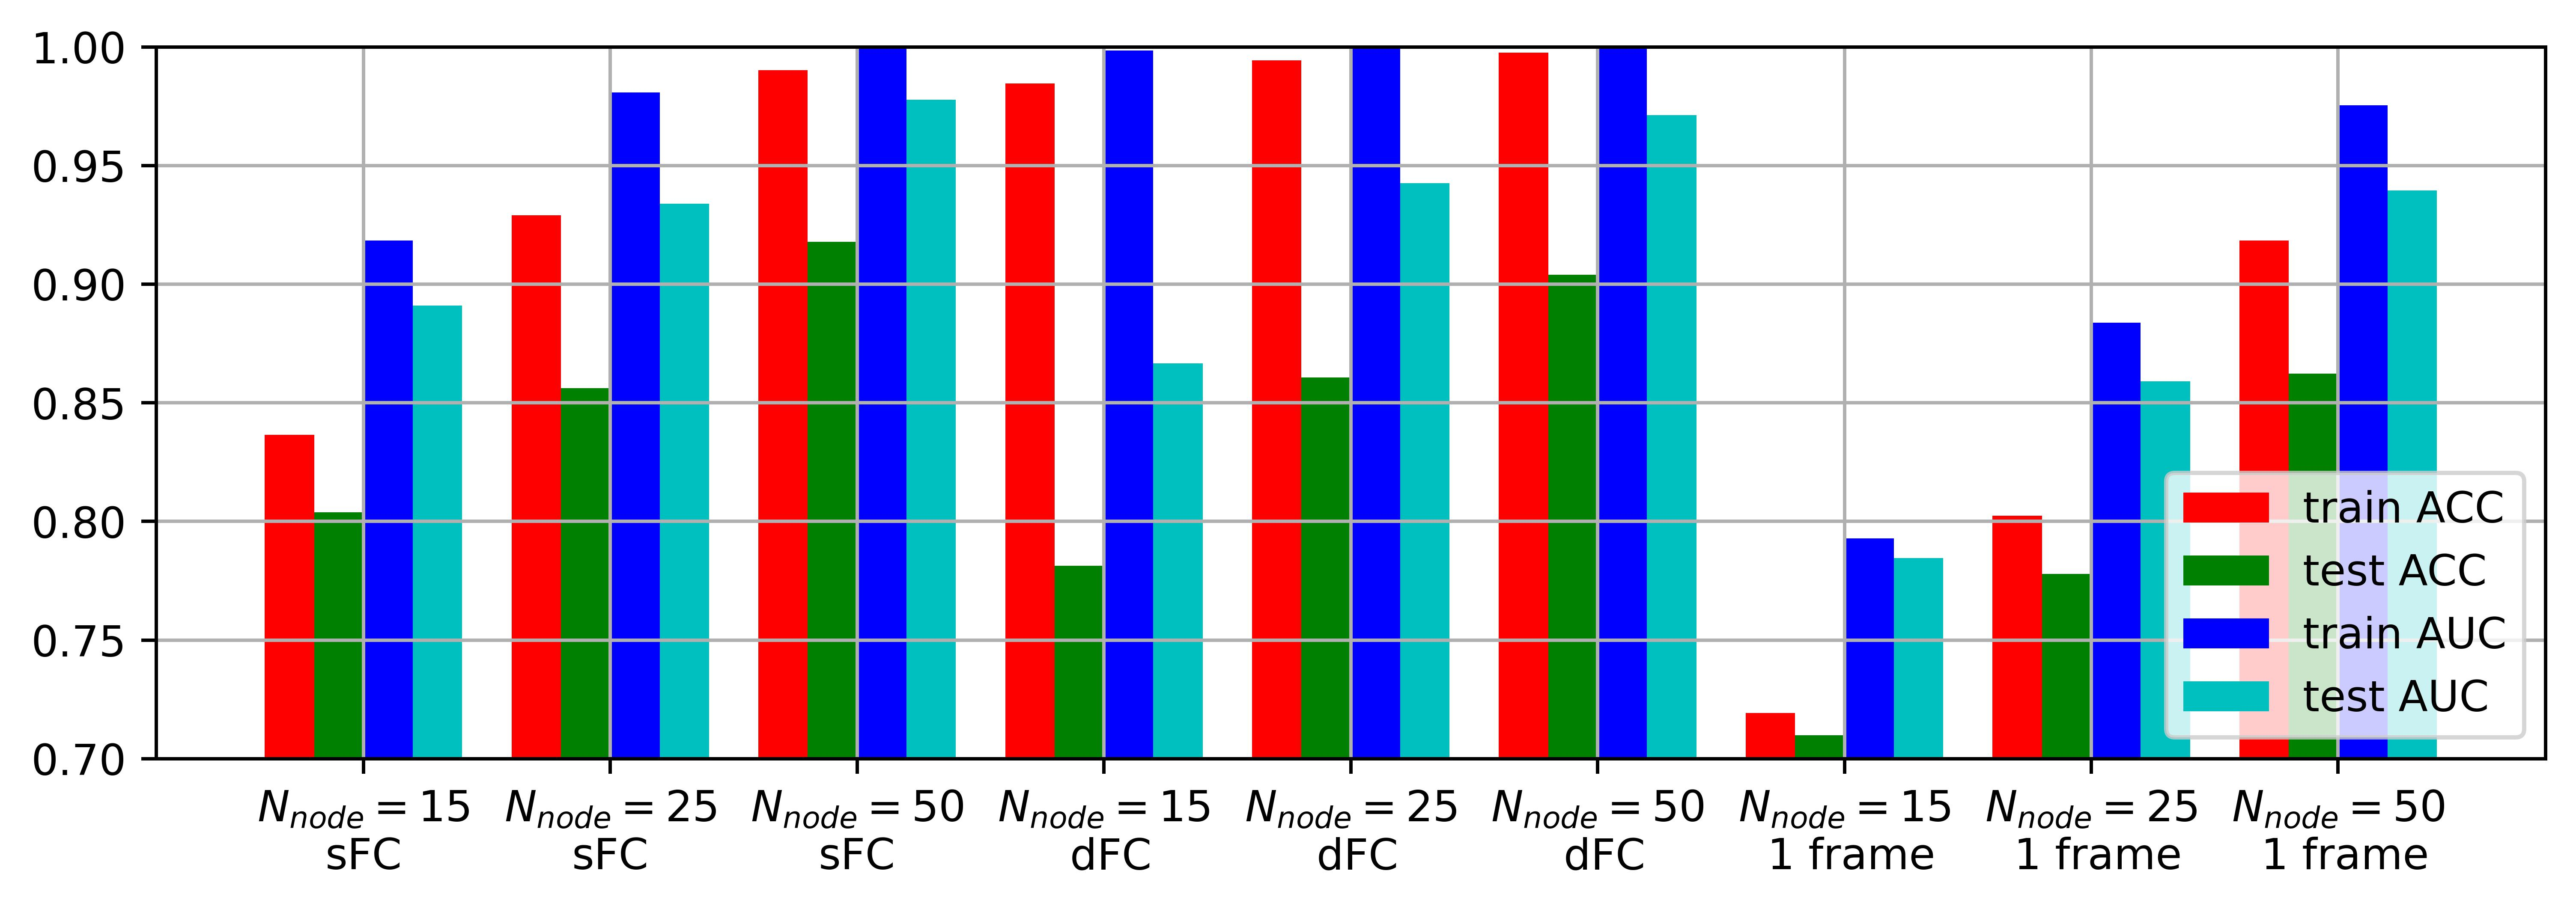
\includegraphics[width=0.8\textwidth]{../Result/bar_channel=4_dropout=0.1.jpg} \\
    \subfloat[test ACC]{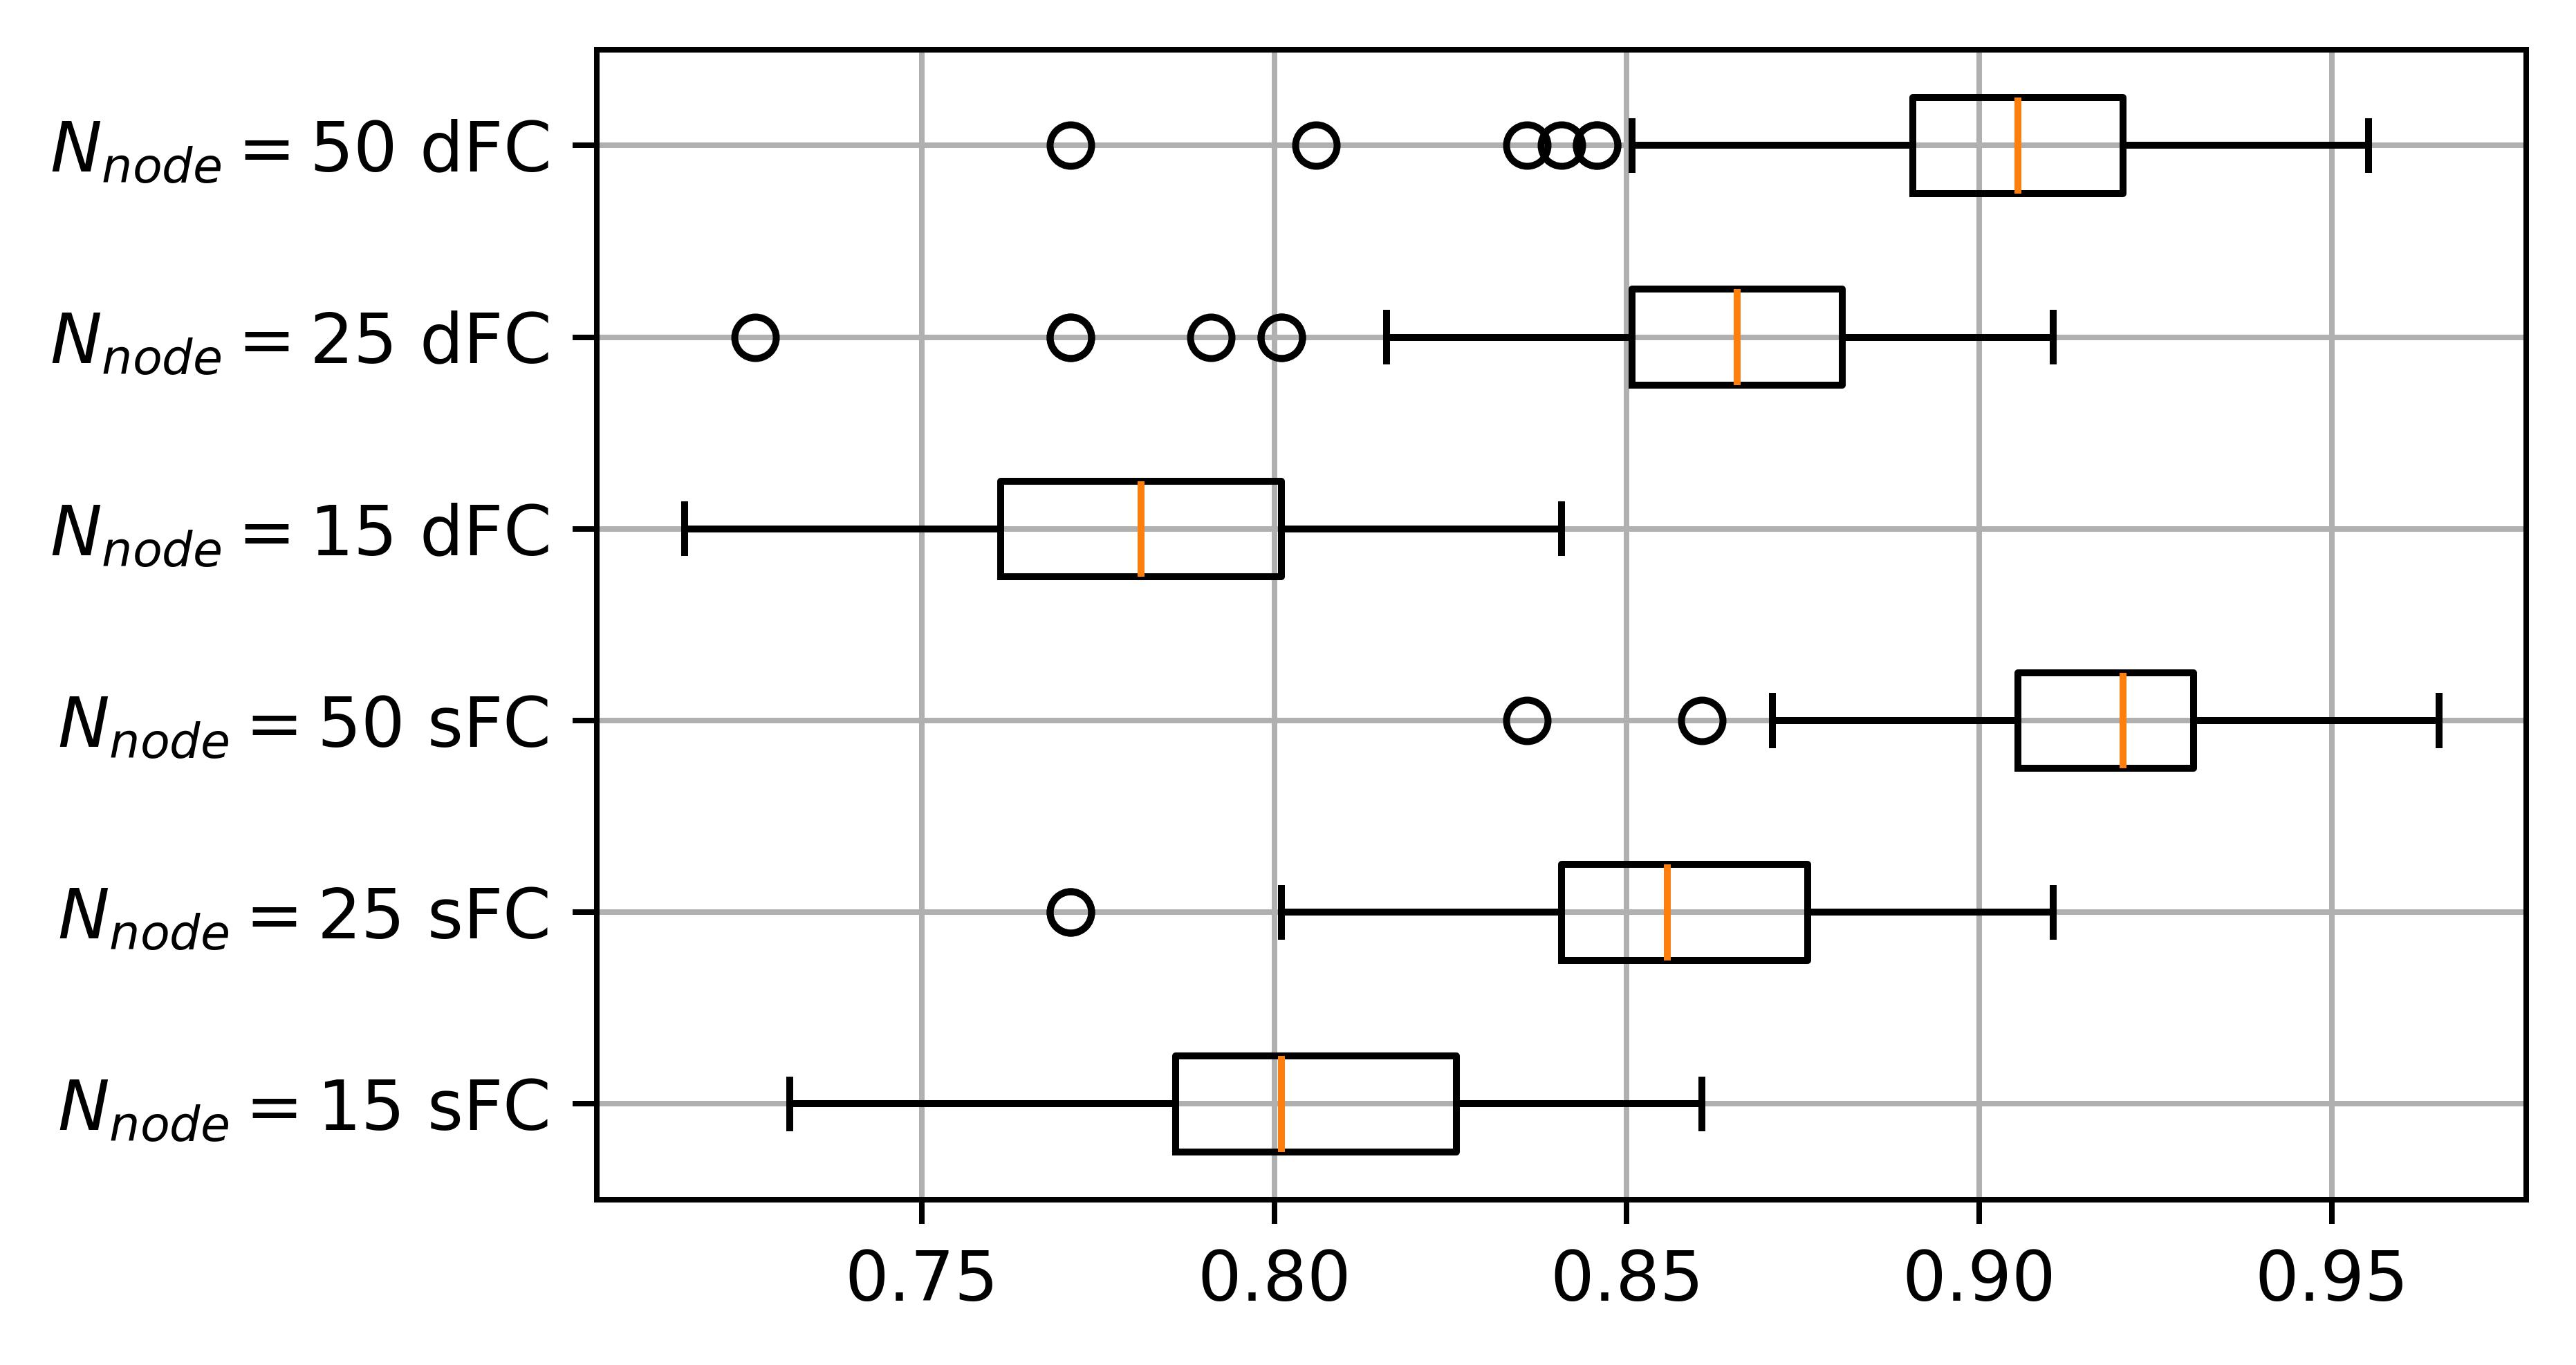
\includegraphics[width=0.4\textwidth]{../Result/test_acc_box_channel=4_dropout=0.1.jpg}}
    \subfloat[test AUC]{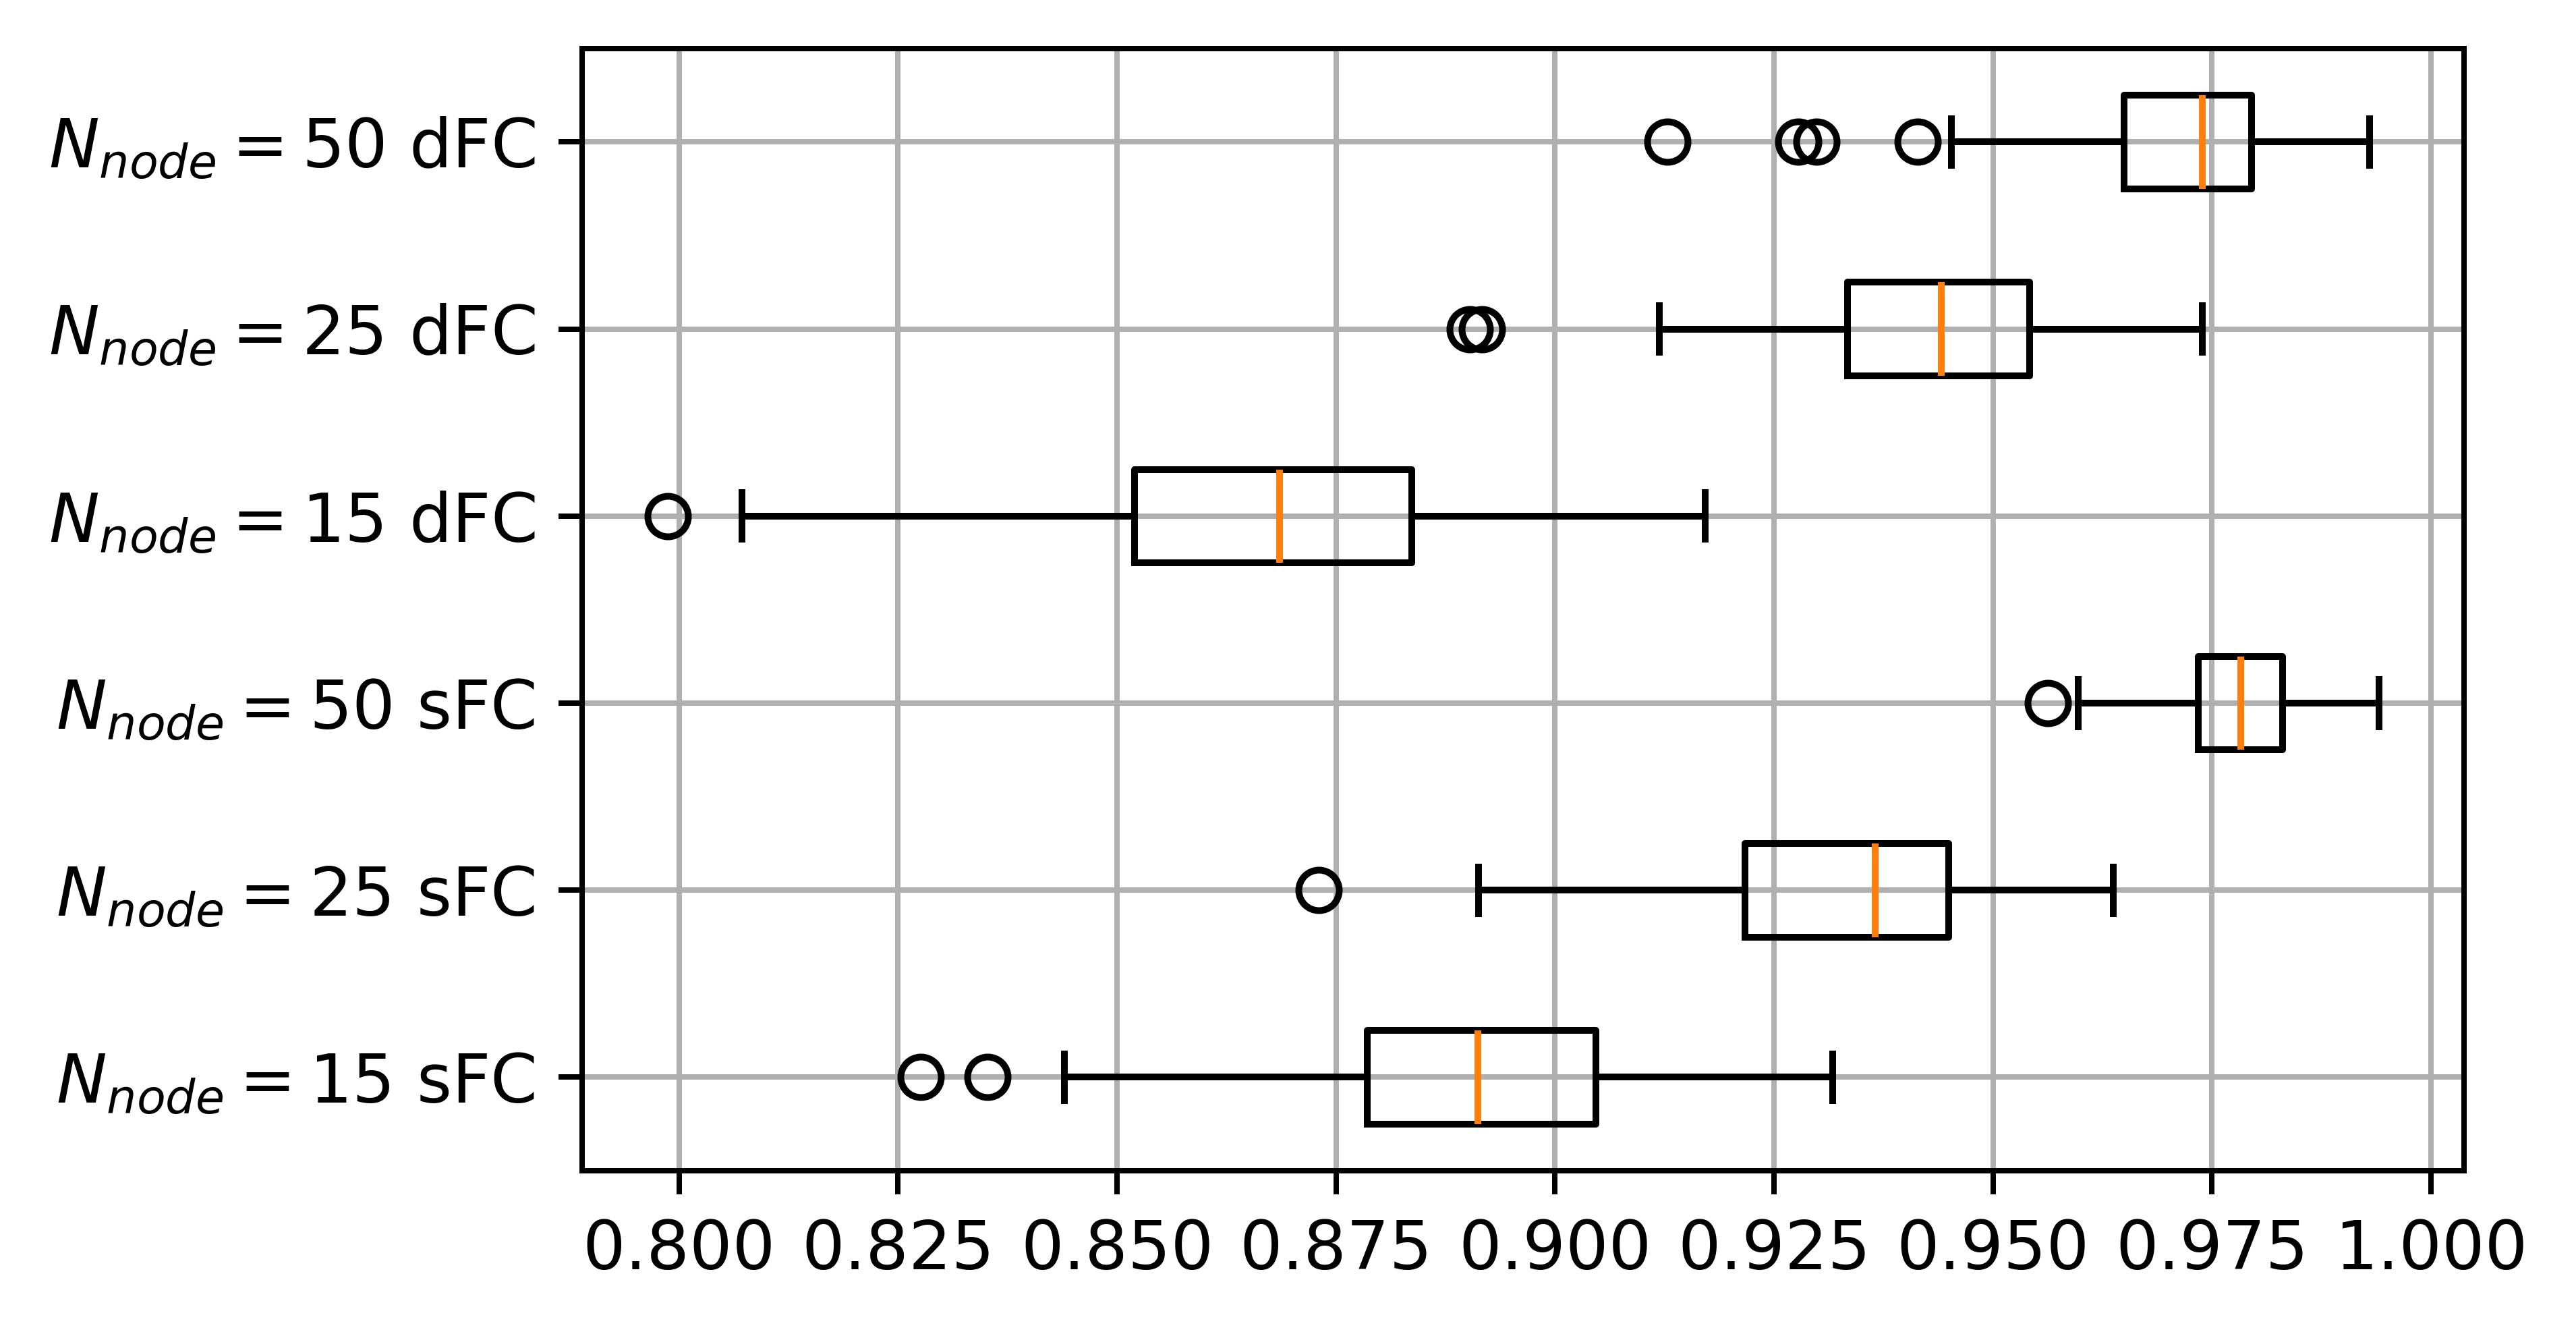
\includegraphics[width=0.4\textwidth]{../Result/test_auc_box_channel=4_dropout=0.1.jpg}}
    \caption{Results of CNN model with dropout = 0.1 and channel = 4.}
    \label{CNN-results}
\end{figure}

The appendix \ref{Ablation-study-for-CNN-model} shows detailed accuracy with all the frame data. In general, classification accuracy still grows with the increase of the number of nodes. However, when comparing the classification accuracy from data with the same nodes, we find that the number of output channels, whether to use dropout normalization, and even using different states of brain network data show little difference in the average and highest accuracy. At 15 nodes, the average AUC and maximum AUC are around 87\% and 92\% respectively. At 25 nodes, these values are around 93\% and 97\%. At 50 nodes, these values are around 97\% and 99\%. The differences in above conditions mainly affect the value of the lowest classification accuracy. To be more specific, when the number of output channels increases or the dropout normalization is not used, the lowest value will be slightly higher than that of other conditions. But it keeps almost the same when processing different states of data with controlling other above experimental conditions, which means that the dynamic data does not perform much better than static data although we try to extract more dynamic features.

\section{Analysis}

\subsection{Linear discriminant analysis (LDA)}

To gain a deeper understanding of the data distribution and find out which brain regions play important roles in classification, we processed the brain network data with linear discriminant analysis (LDA) \cite{Goldstein1976-aj}, which is used as a statistical method to find the optimal linear combination to maximise between-group variance and minimise within-group variance. Specifically, for a given dataset $\{\mathbf{x}_i, y_i\}_{i=1}^N$, the LDA method aims to find a vector pair $\mathbf{w}, \mathbf{c}$ such that the inner product $\langle \mathbf{x}_i  - \mathbf{c}, \mathbf{w} \rangle$ minimizes the interclass variance and maximizes the distance between the projected means of the classes.

Figure \ref{LDA-example-sfc} and Figure \ref{LDA-example-dfc} shows the distributions of static and dynamic functional connectivity with different nodes, from which we can gain the following conclusions: (1) there are overlapping parts in the data distribution of male and female under different nodes, and these regions may represent the common brain network characteristics or functional connectivity patterns of both genders; (2) the area of overlapping parts becomes smaller with the increase of the number of nodes, which supports the conclusions that more nodes lead to more higher accuracy and AUC in section 2; (3) there are outliers presents in both dynamic and static functional connectivity, with the dynamic functional connectivity exhibiting no fewer outliers than the static data, which might have negative impacts on the experimental results, thereby reducing the accuracy of gender classification especially using dynamic brain network data.


\begin{figure}[H]
    \centering
    \subfloat[$N_{\text{node}} = 15$]{
        \begin{minipage}[b]{0.3\textwidth}
            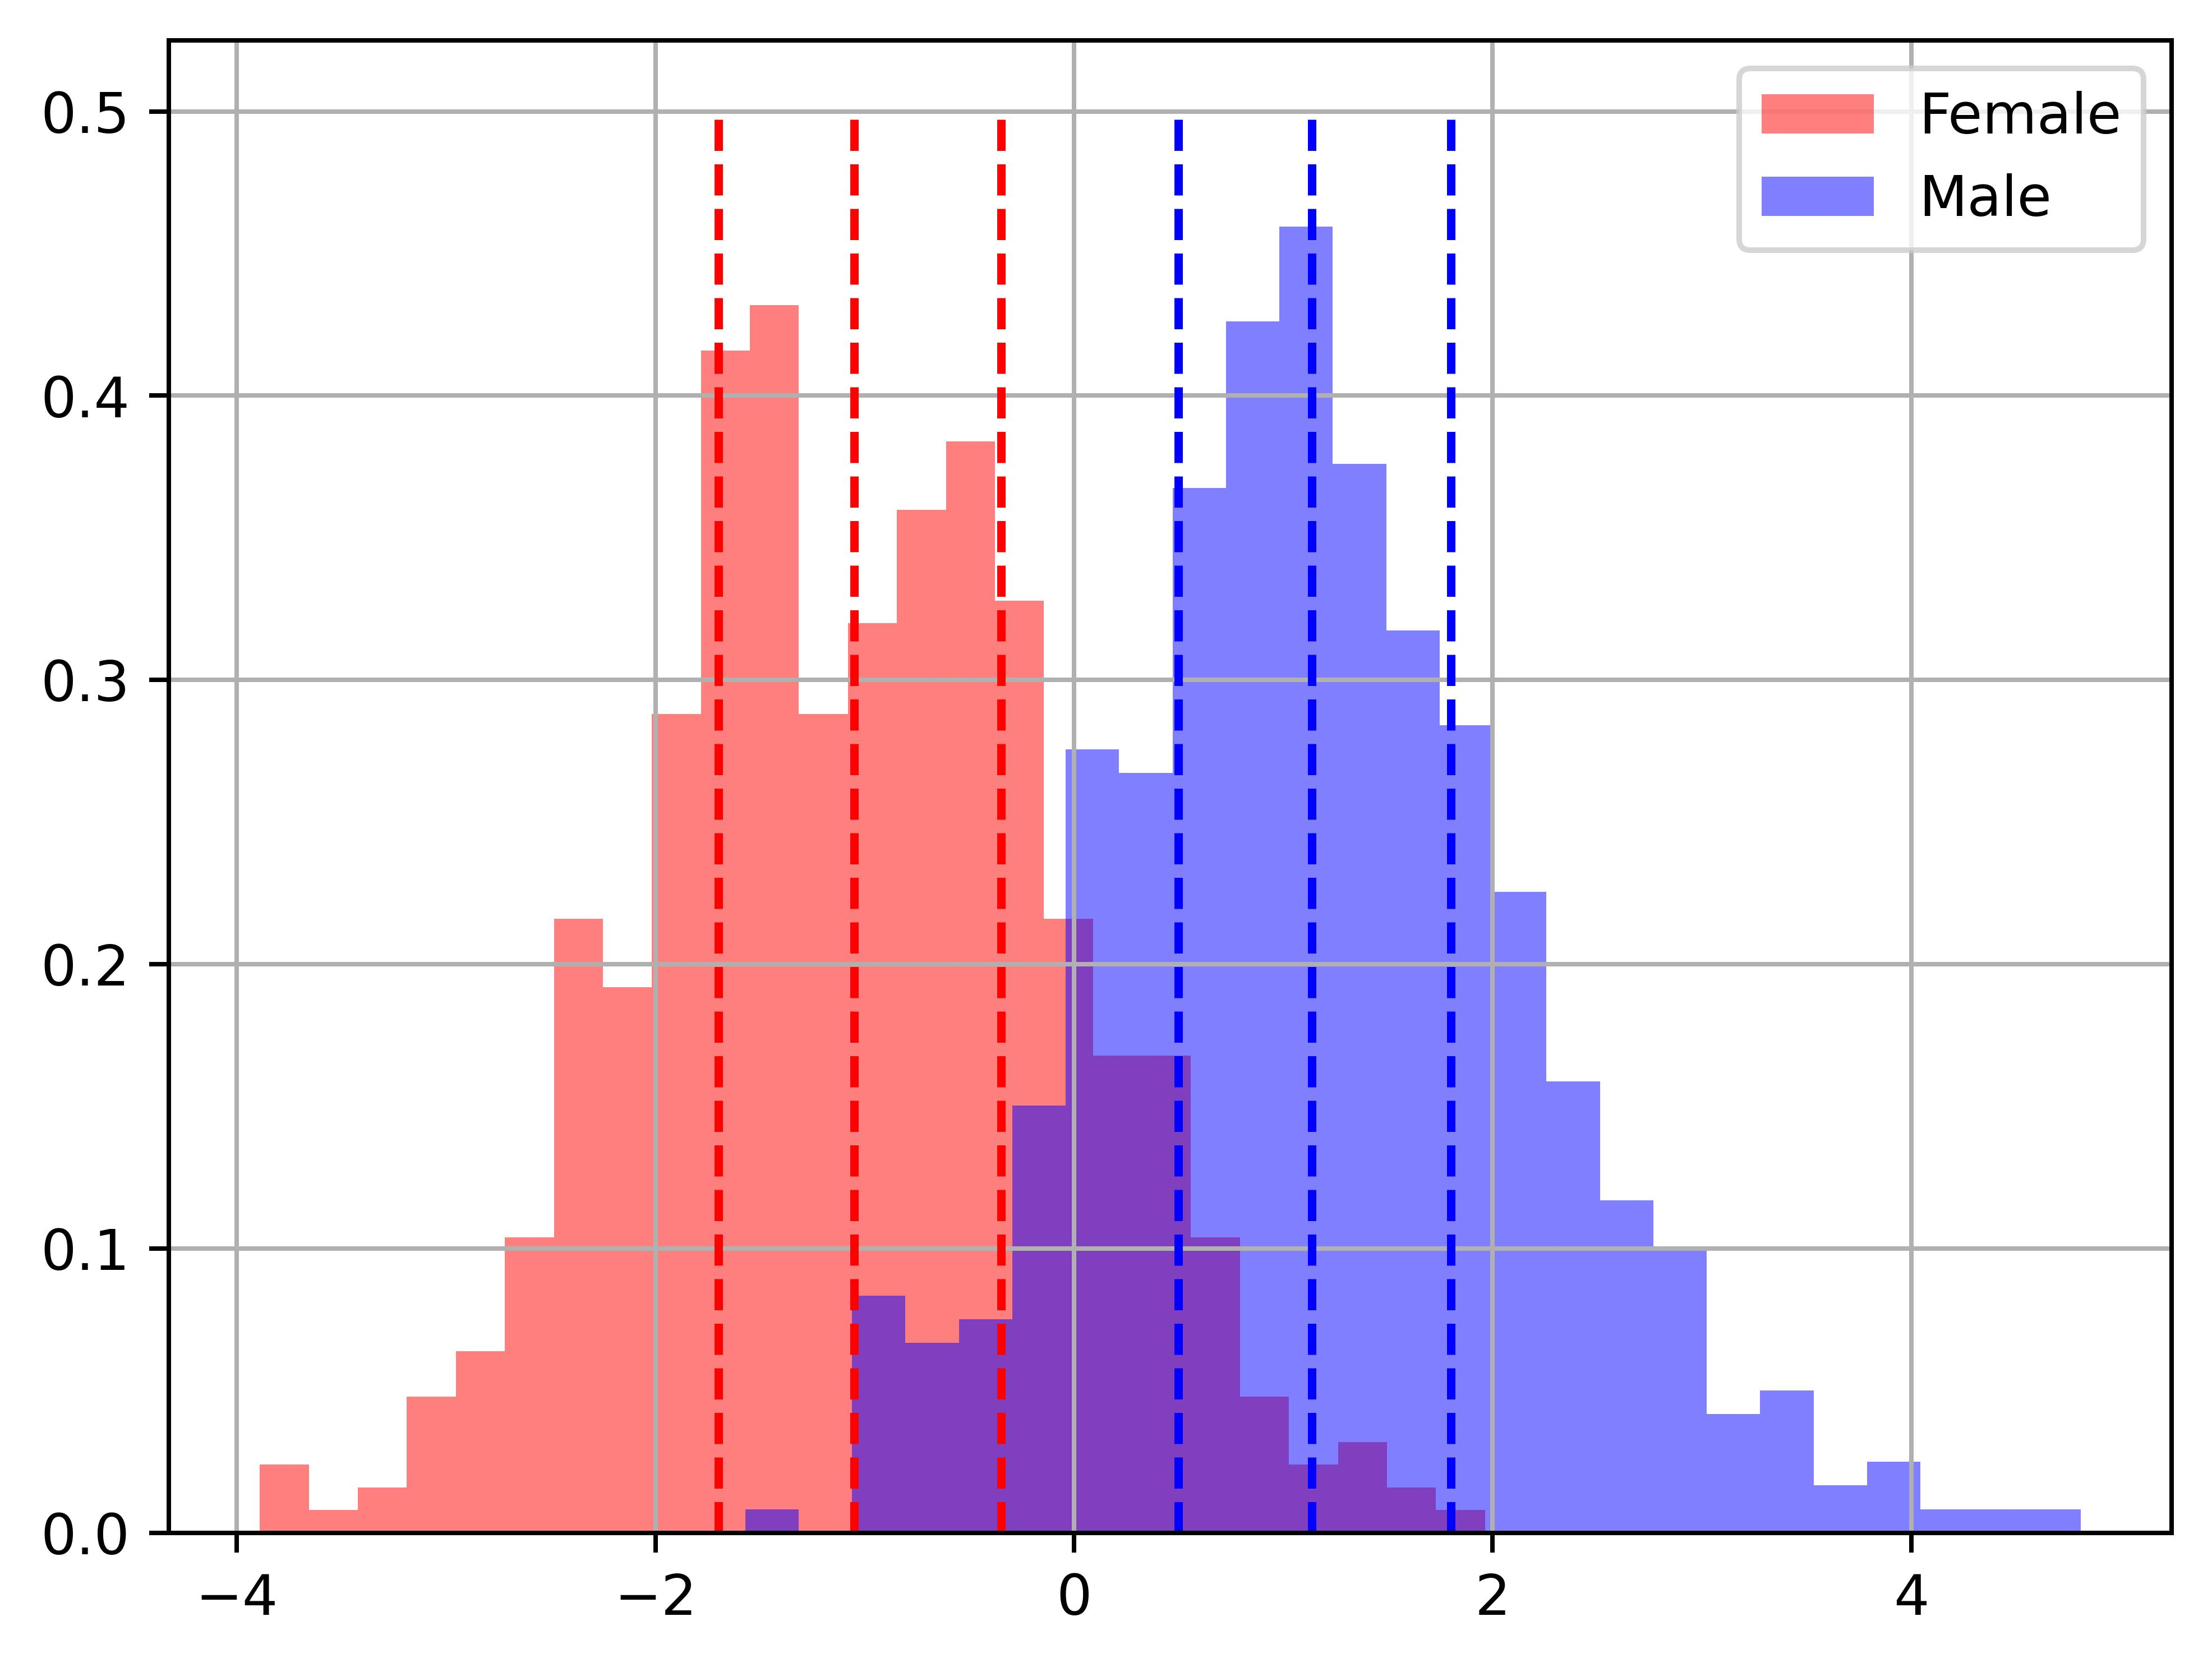
\includegraphics[width=1\textwidth]{../Analysis/LDA/node=15_size=4800_step=4800_rho=0.1/hist_0.jpg}
            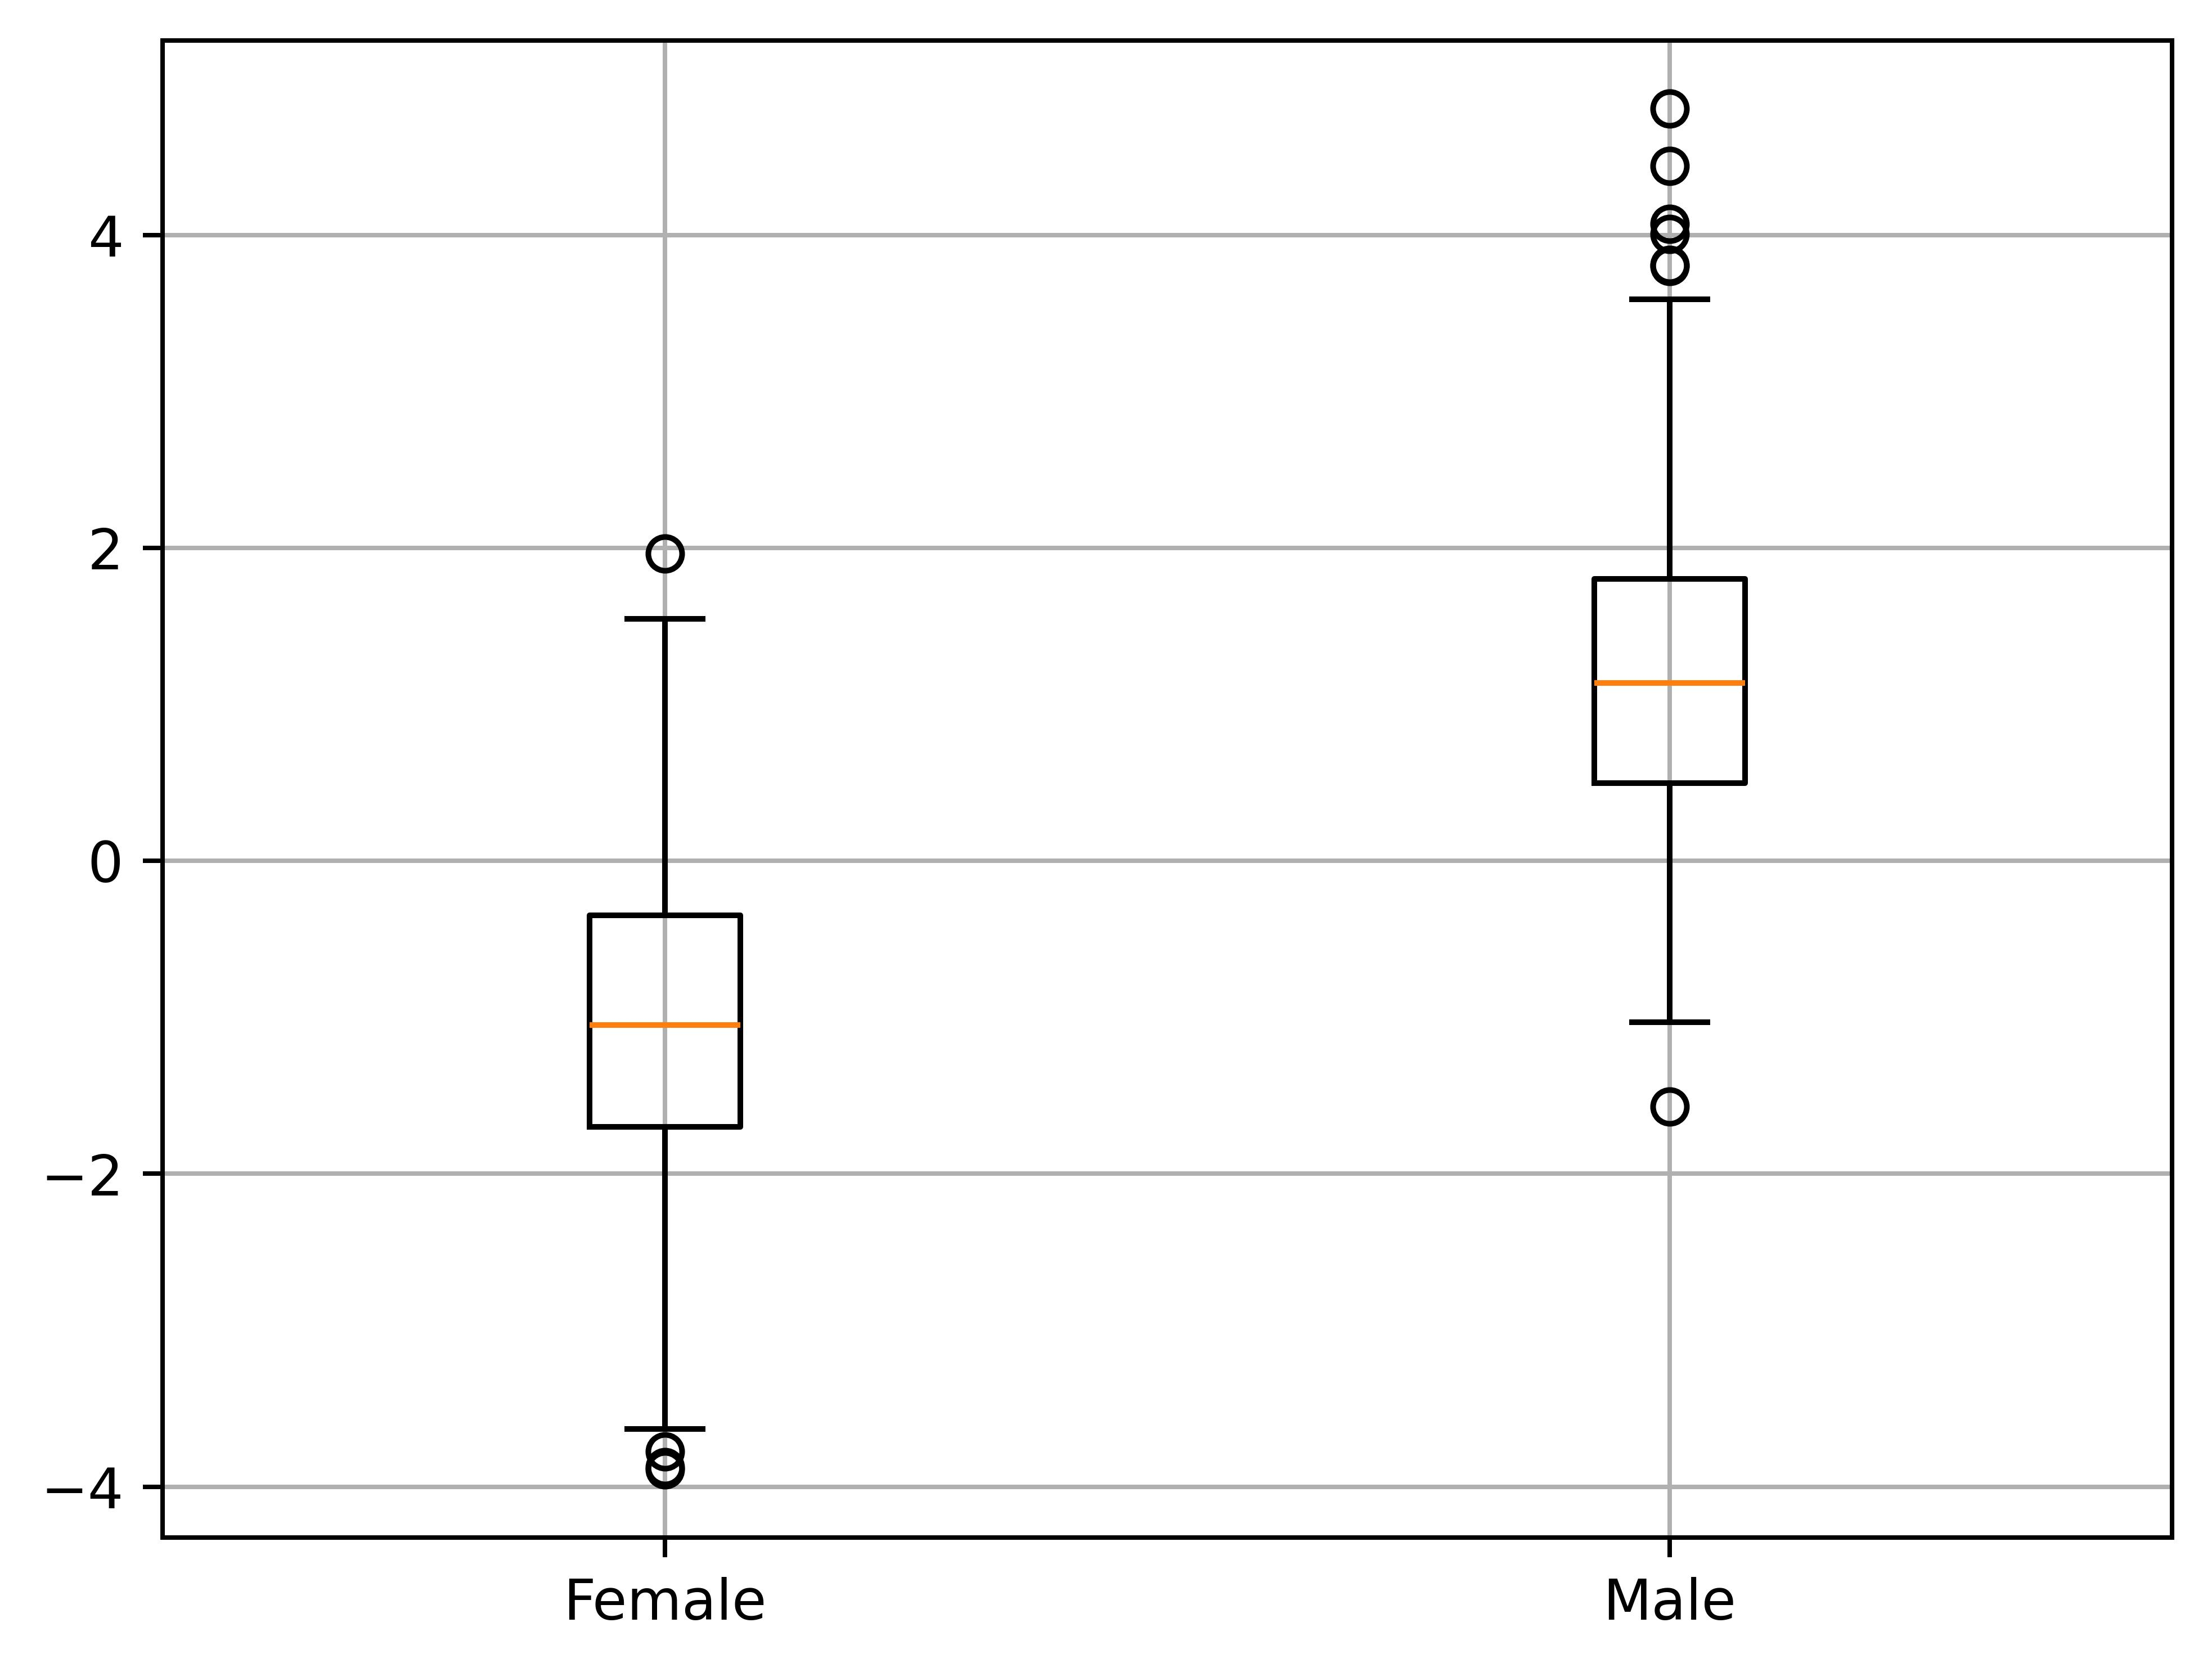
\includegraphics[width=1\textwidth]{../Analysis/LDA/node=15_size=4800_step=4800_rho=0.1/box_0.jpg}
        \end{minipage}
    }
    \subfloat[$N_{\text{node}} = 25$]{
        \begin{minipage}[b]{0.3\textwidth}
            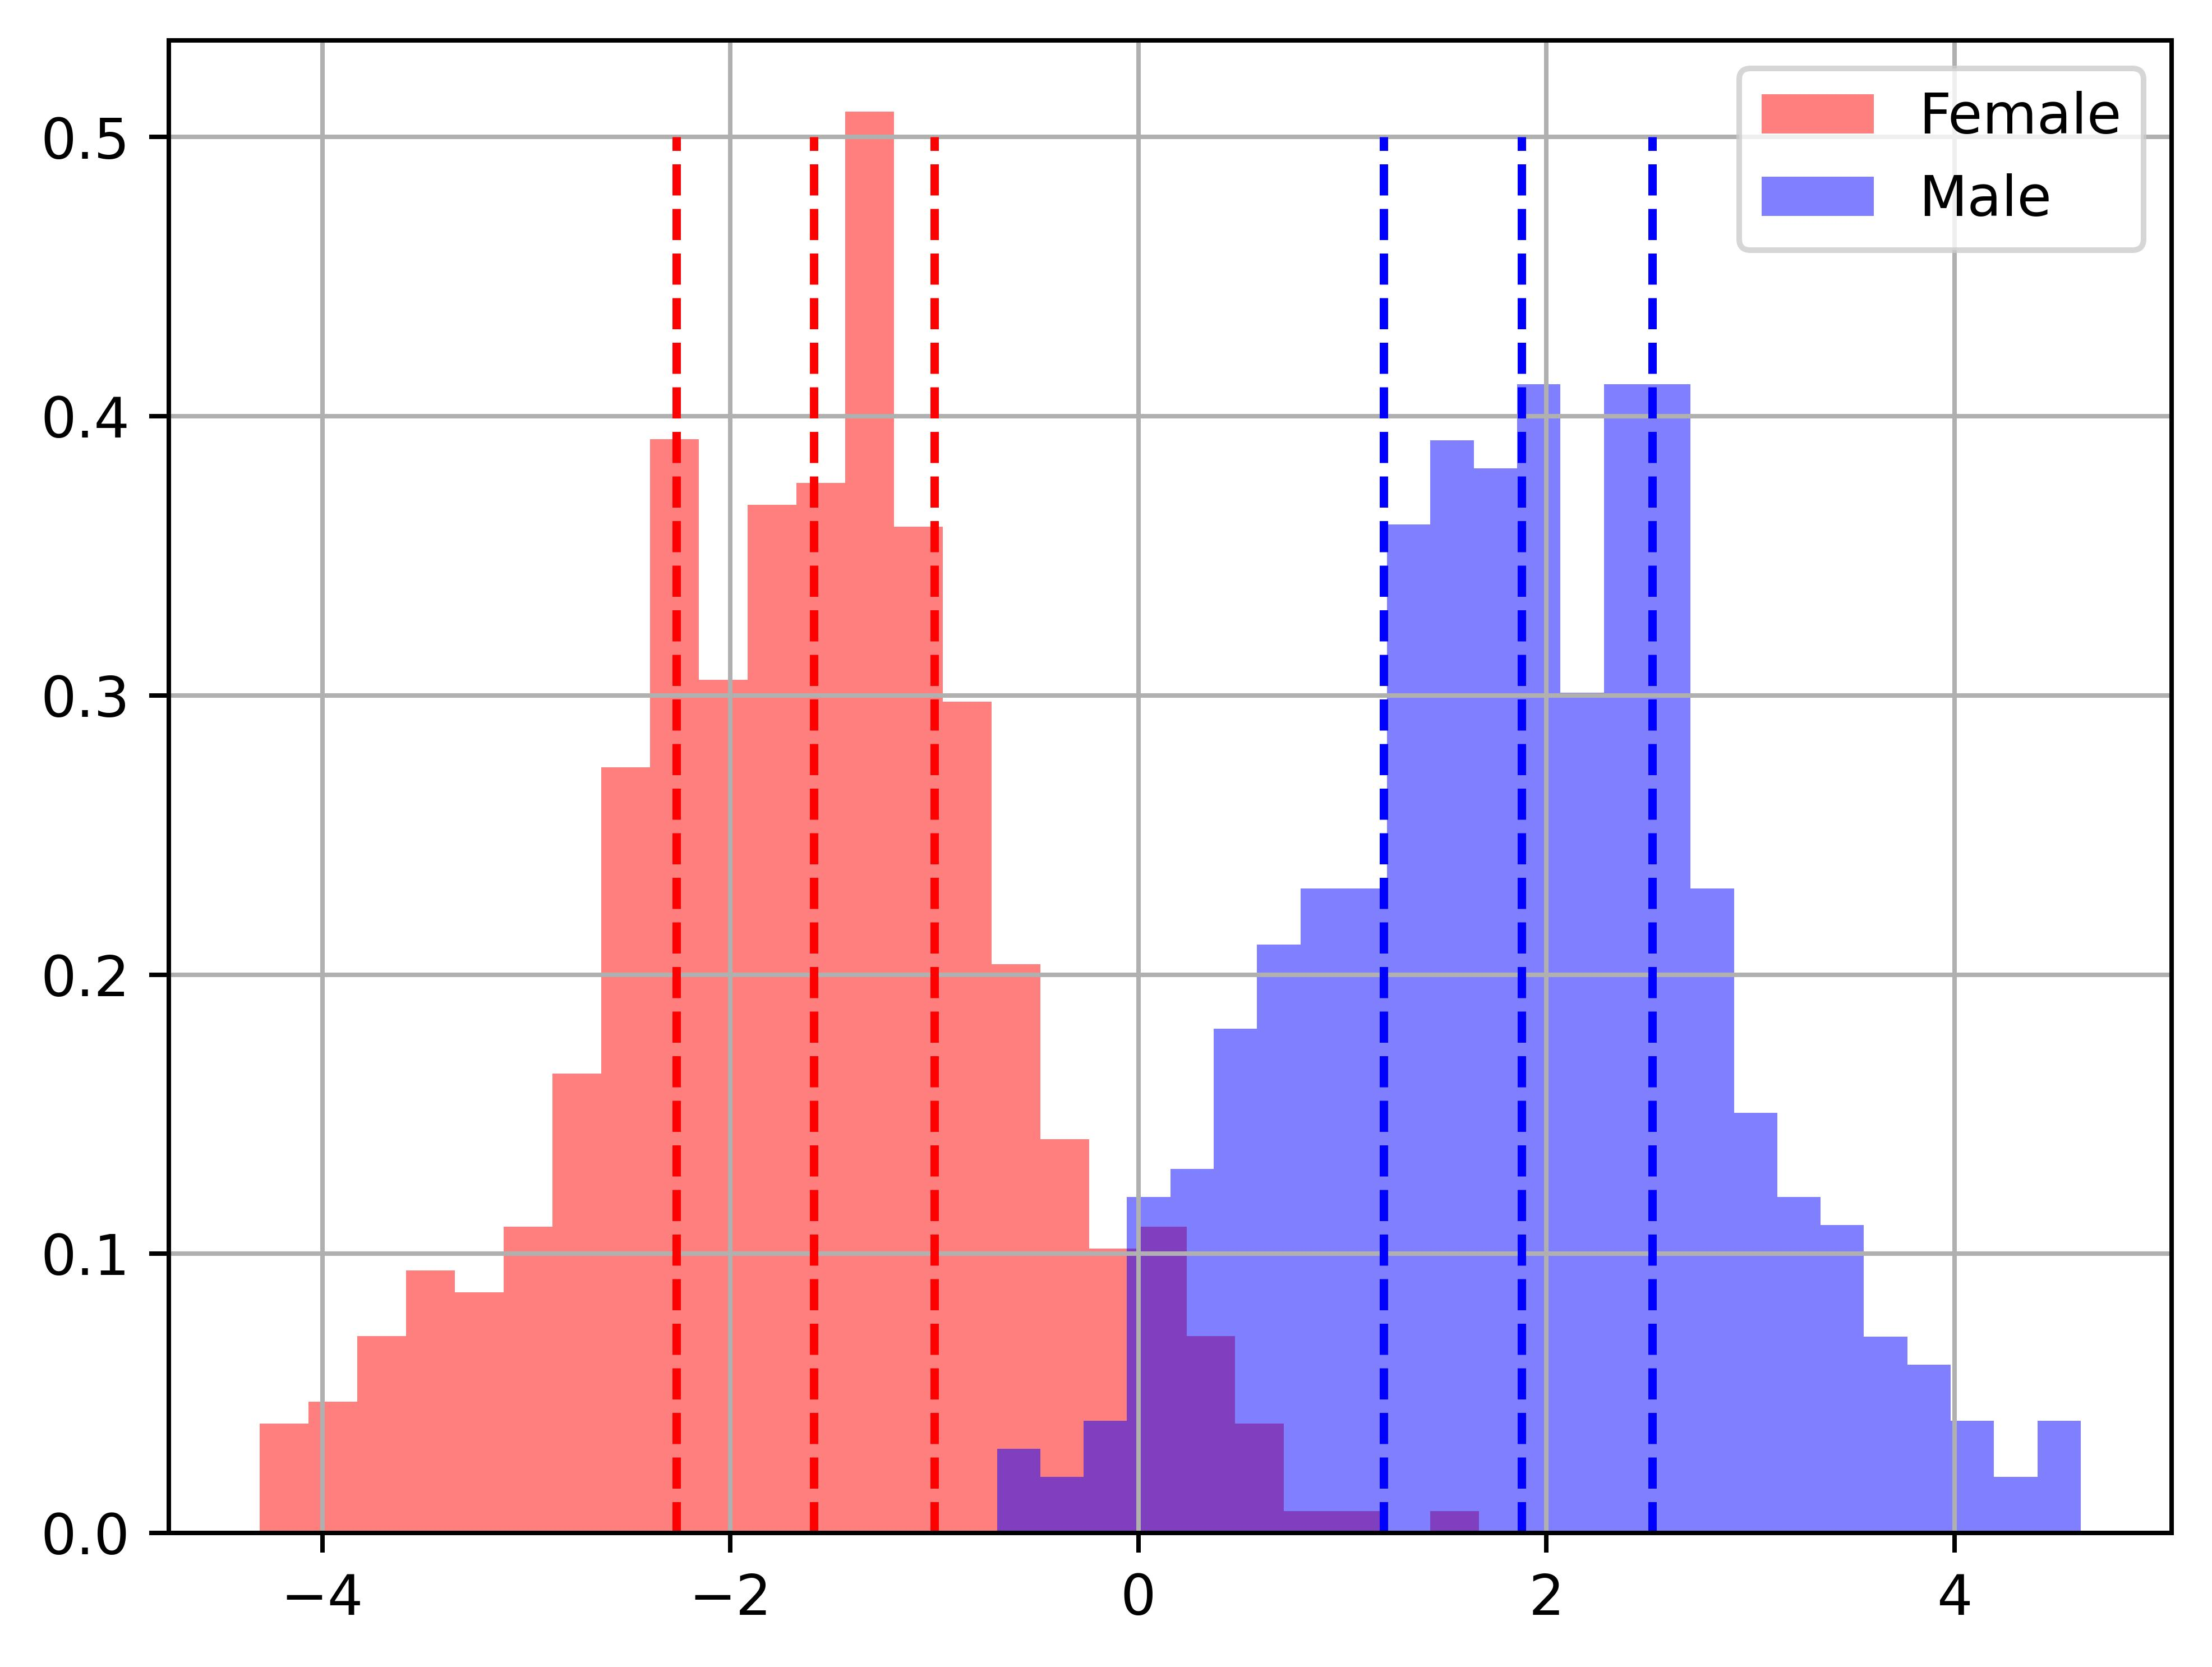
\includegraphics[width=1\textwidth]{../Analysis/LDA/node=25_size=4800_step=4800_rho=0.1/hist_0.jpg}
            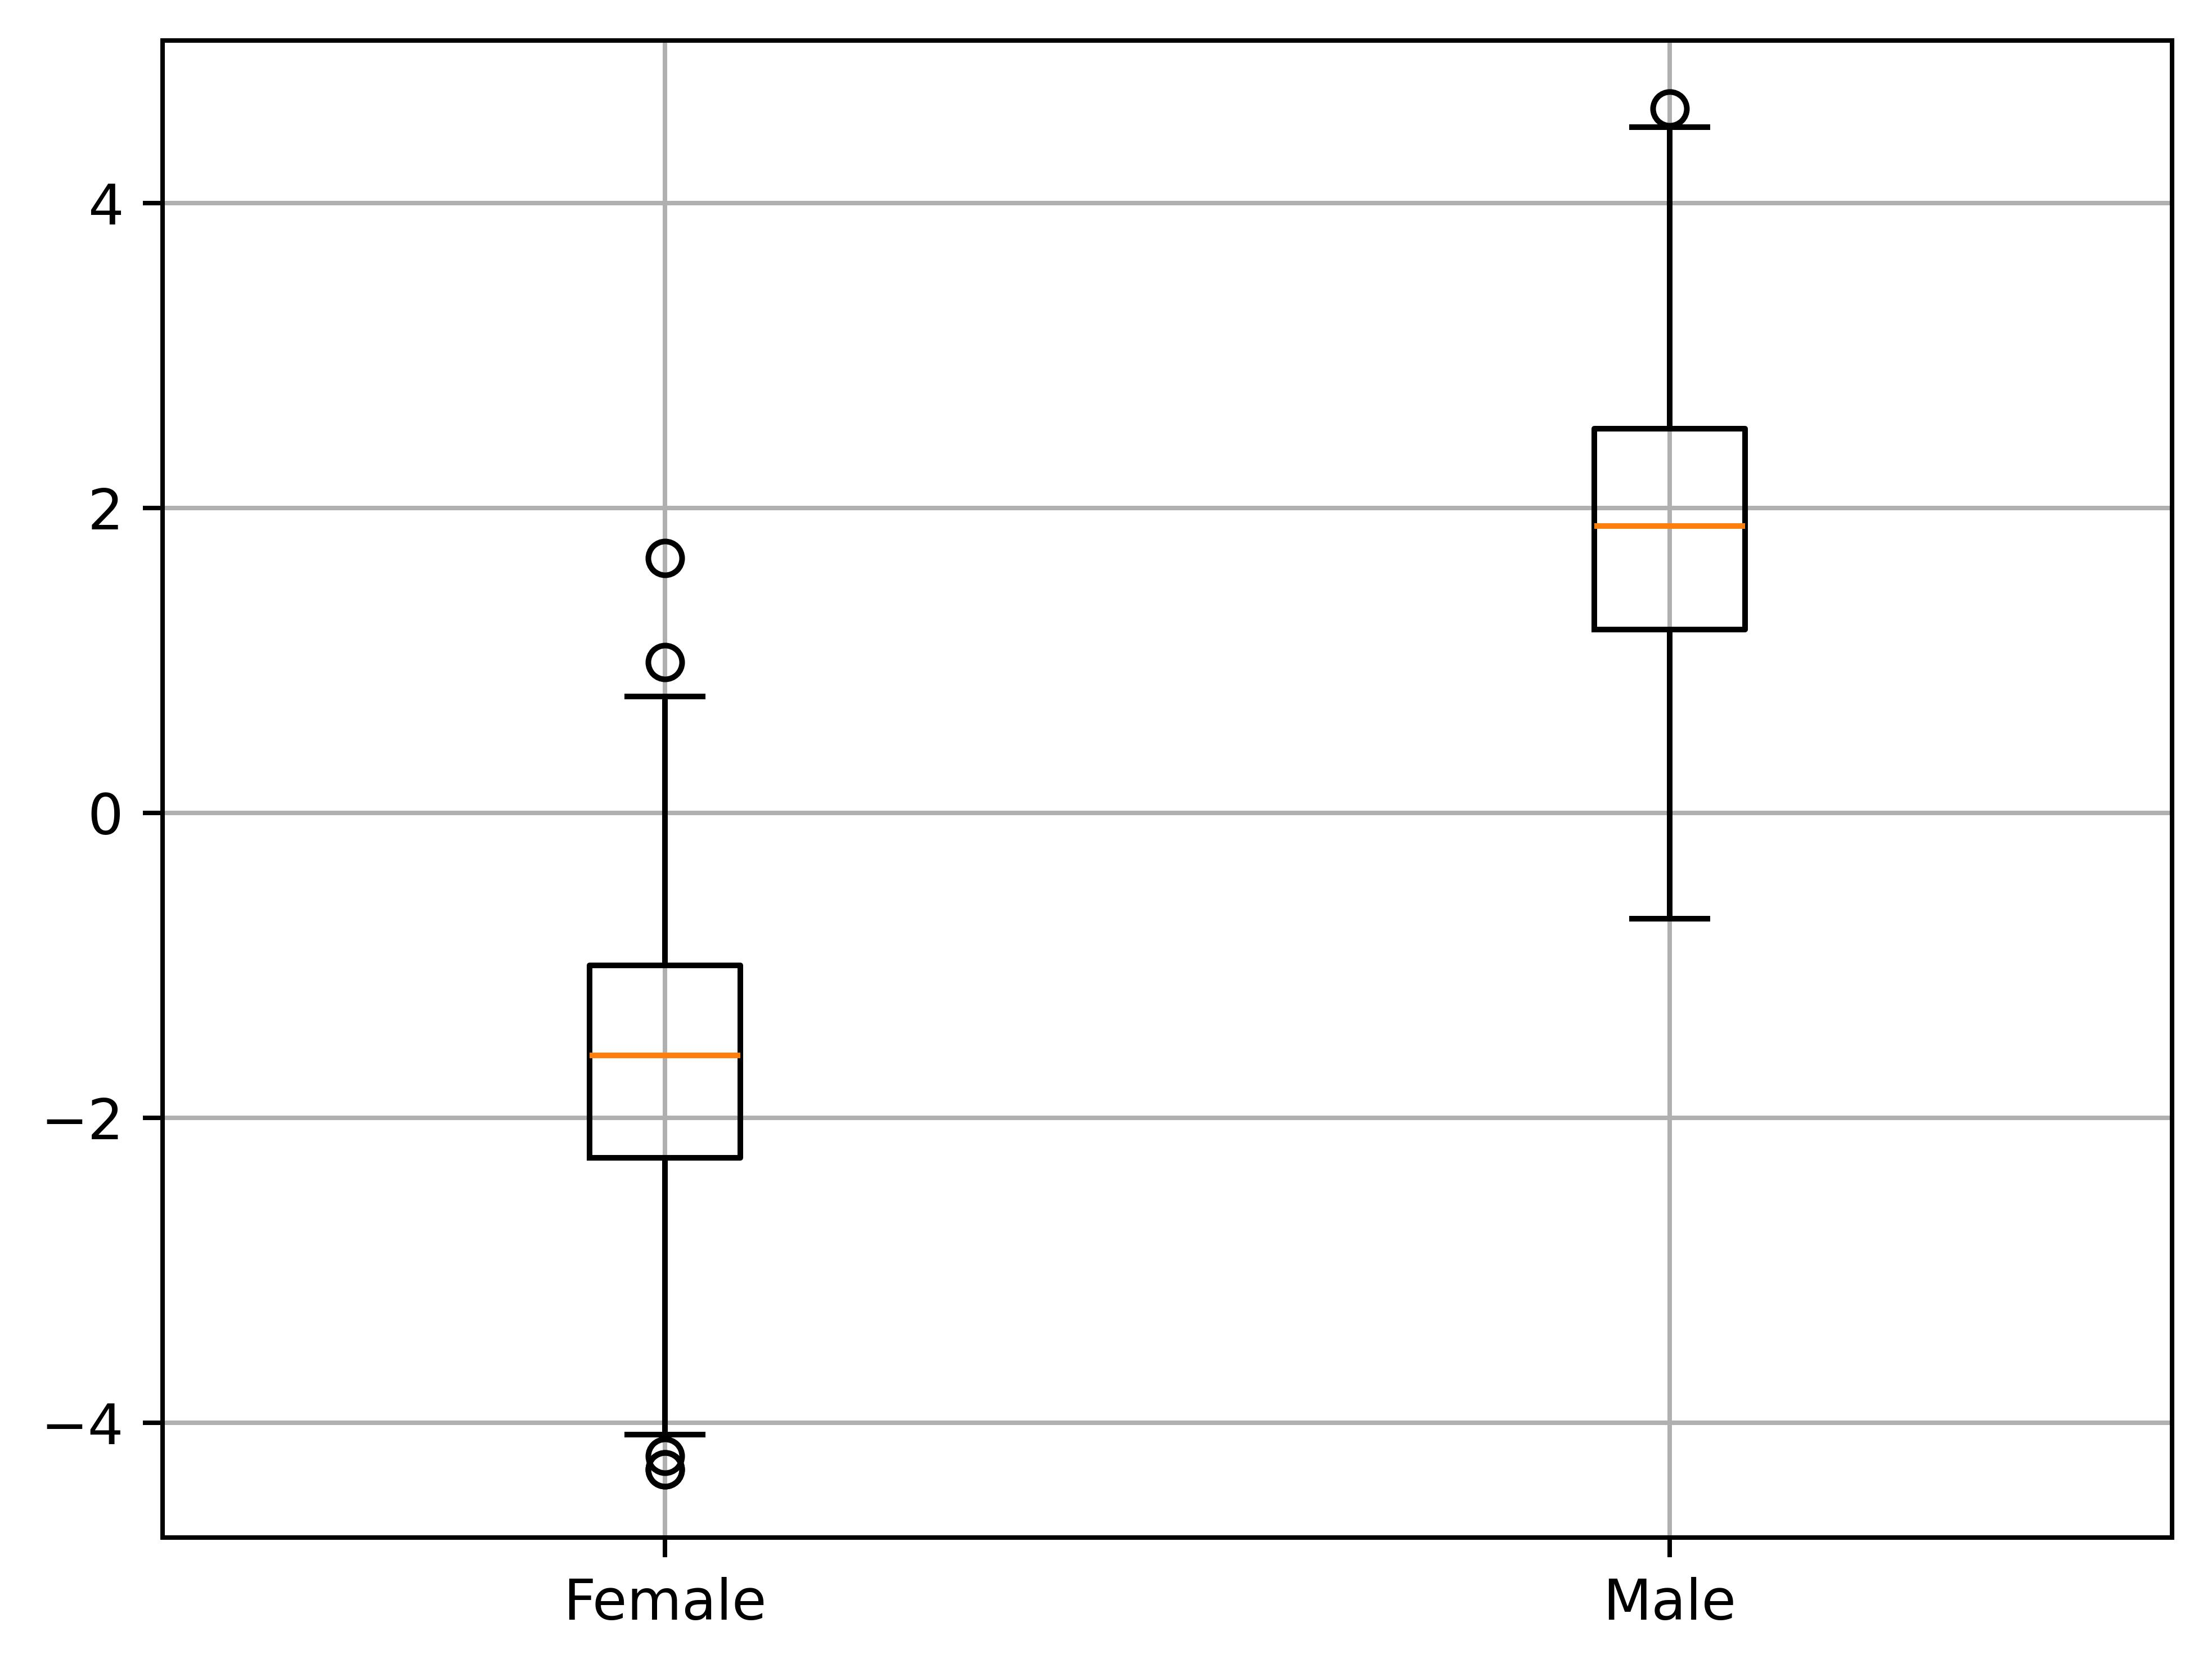
\includegraphics[width=1\textwidth]{../Analysis/LDA/node=25_size=4800_step=4800_rho=0.1/box_0.jpg}
        \end{minipage}
    }
    \subfloat[$N_{\text{node}} = 50$]{
        \begin{minipage}[b]{0.3\textwidth}
            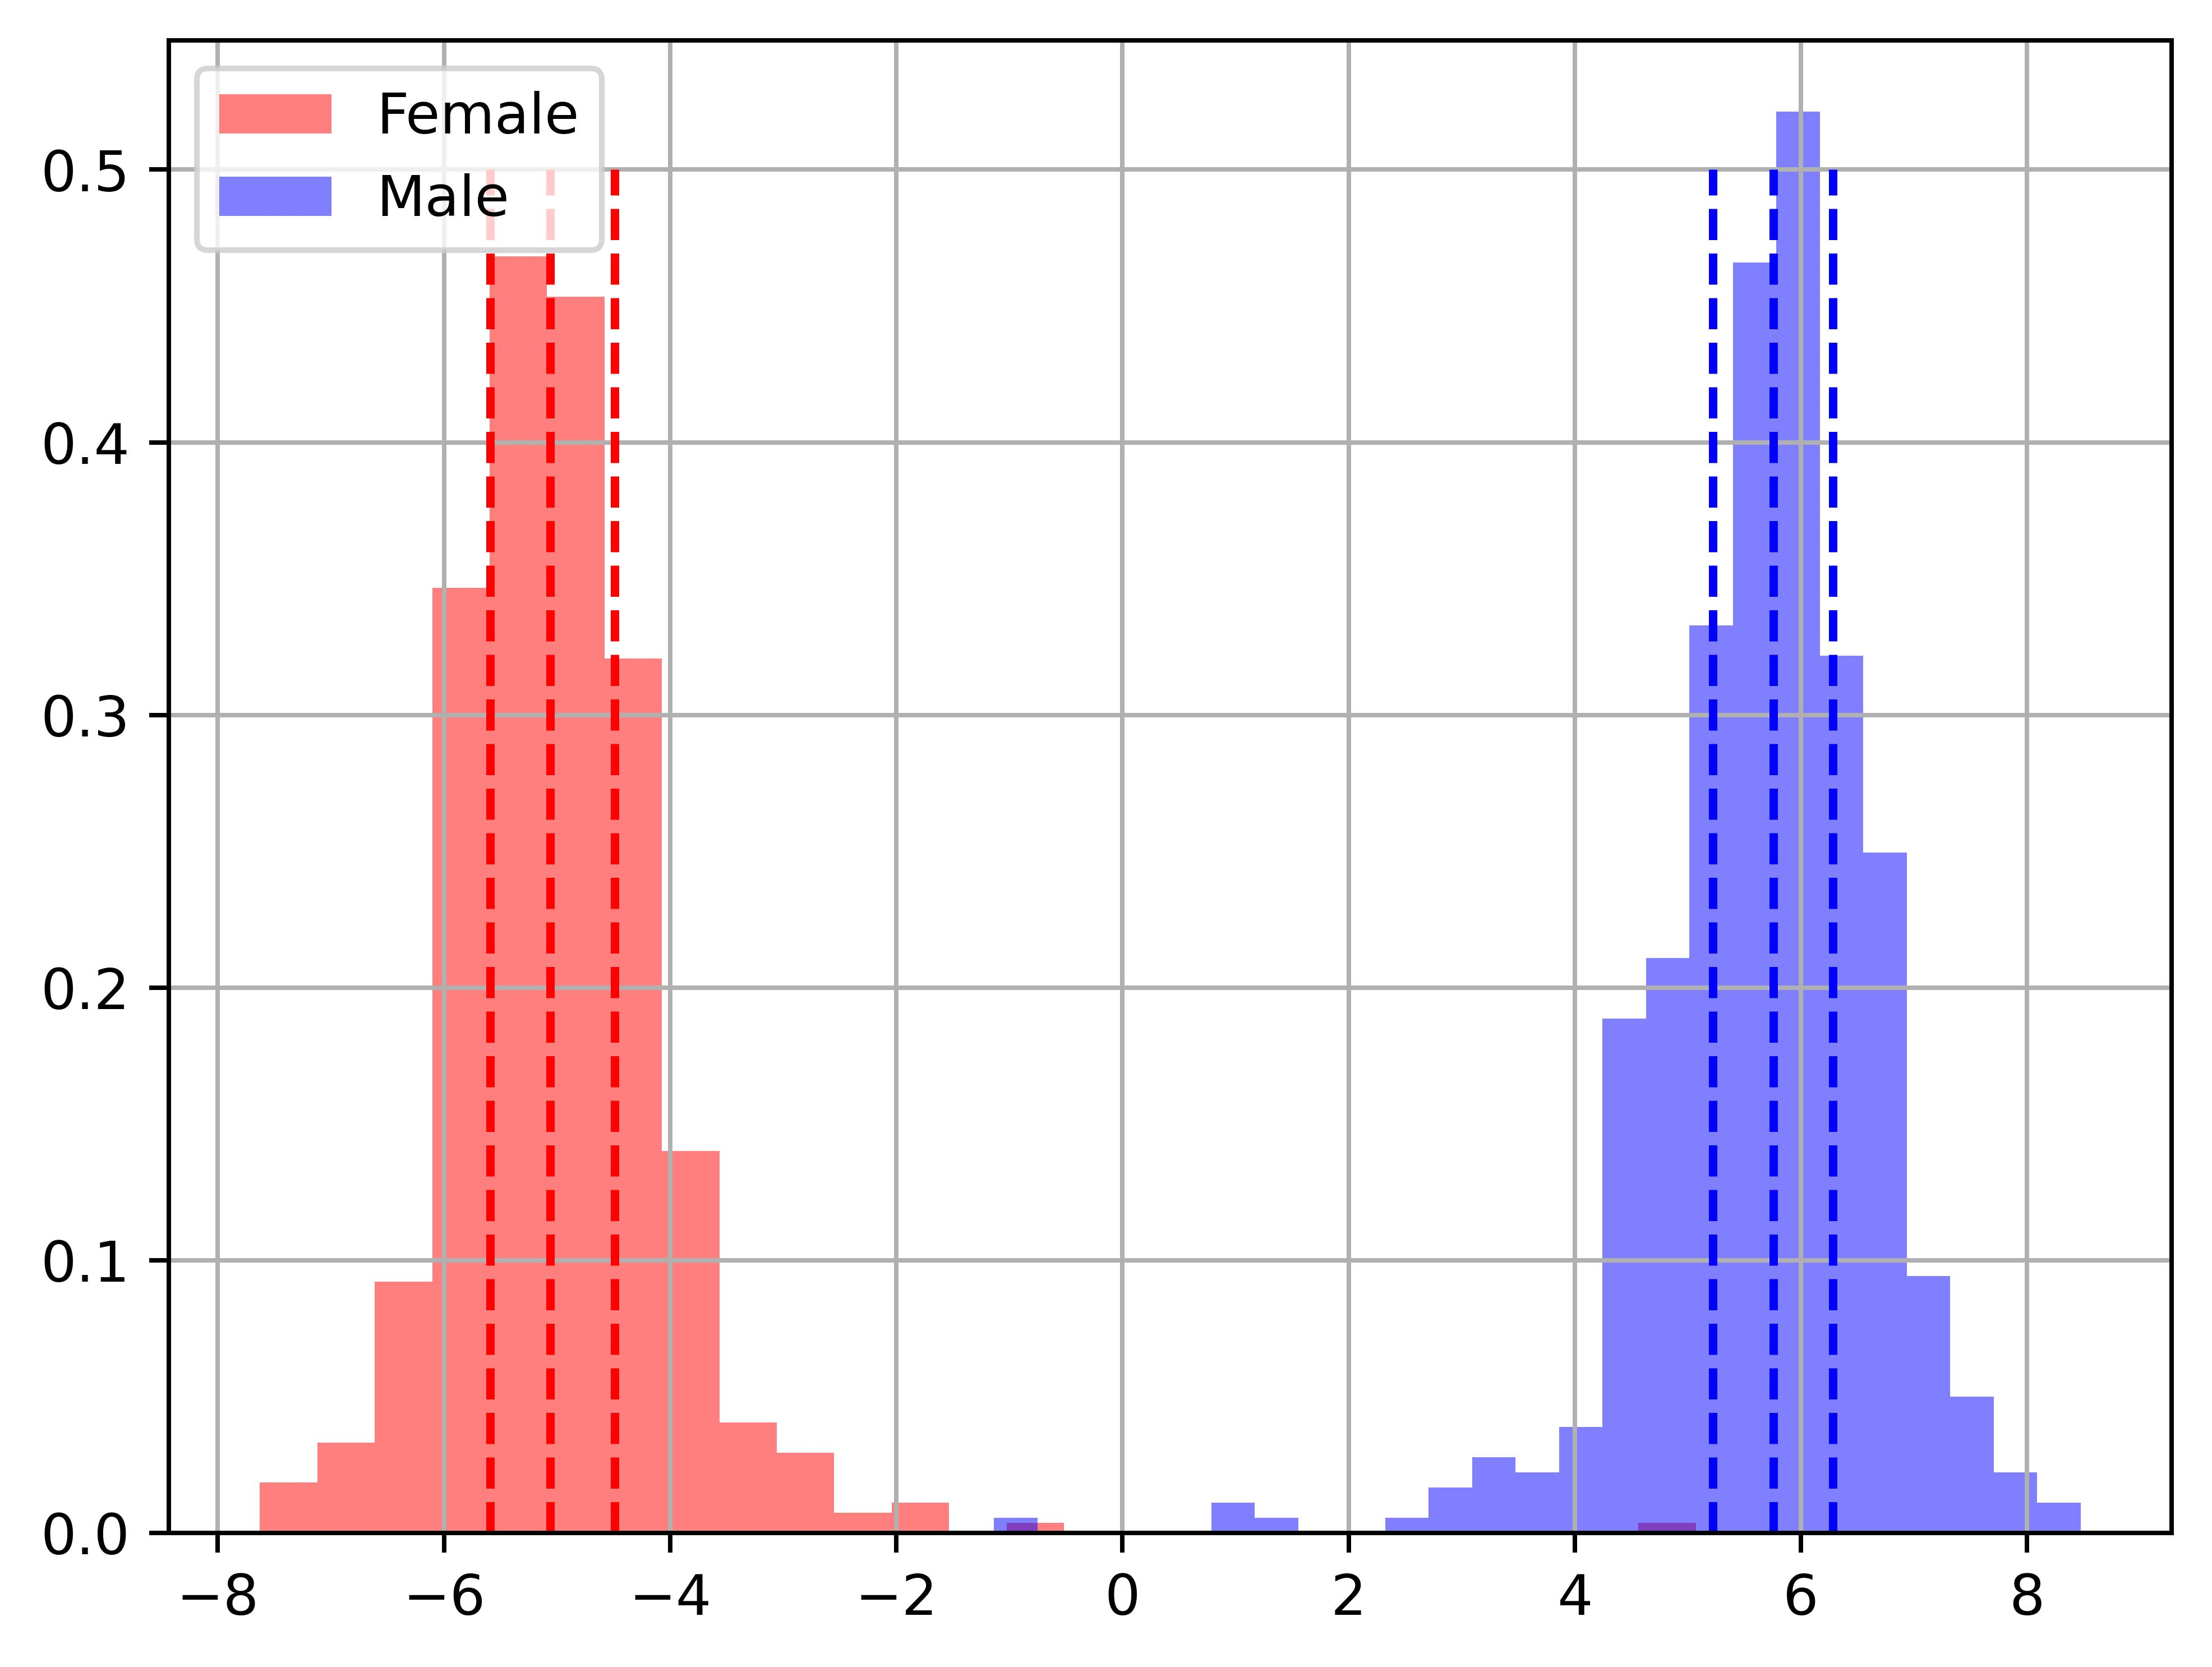
\includegraphics[width=1\textwidth]{../Analysis/LDA/node=50_size=4800_step=4800_rho=0.1/hist_0.jpg}
            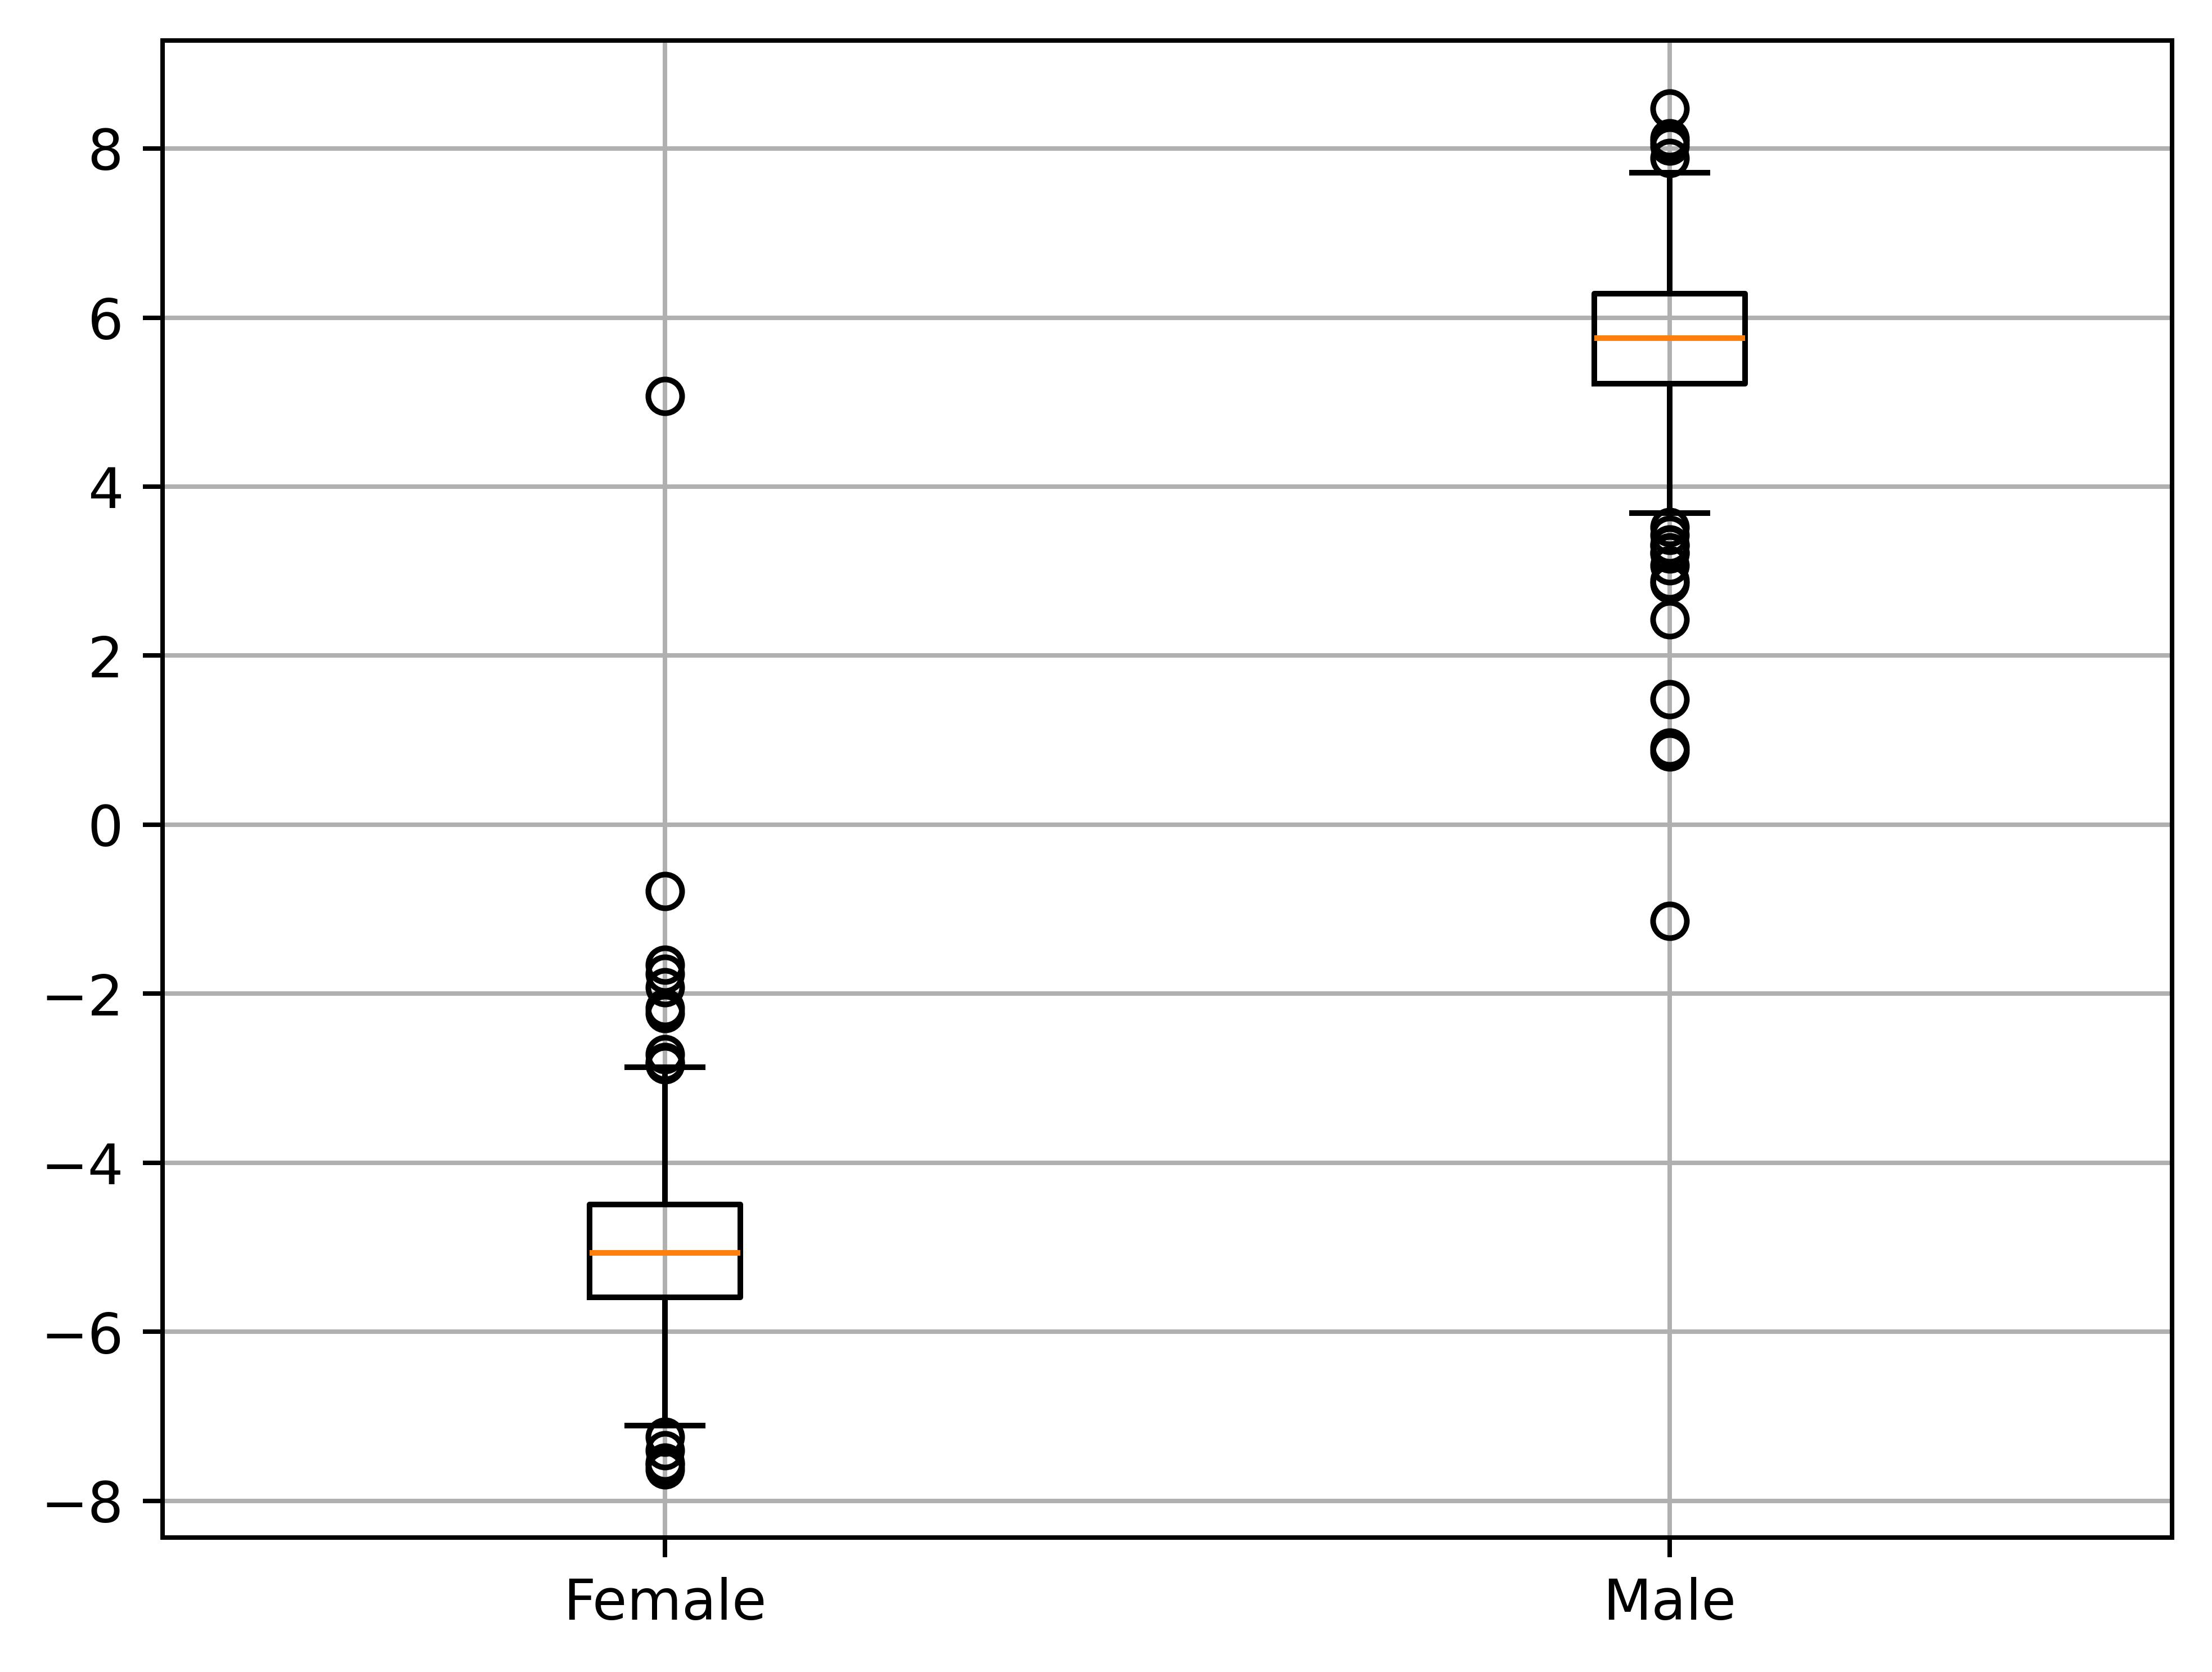
\includegraphics[width=1\textwidth]{../Analysis/LDA/node=50_size=4800_step=4800_rho=0.1/box_0.jpg}
        \end{minipage}
    }
    \caption{LDA for sFC.}
    \label{LDA-example-sfc}
\end{figure}

\begin{figure}[H]
    \centering
    \subfloat[$N_{\text{node}} = 15$]{
        \begin{minipage}[b]{0.3\textwidth}
            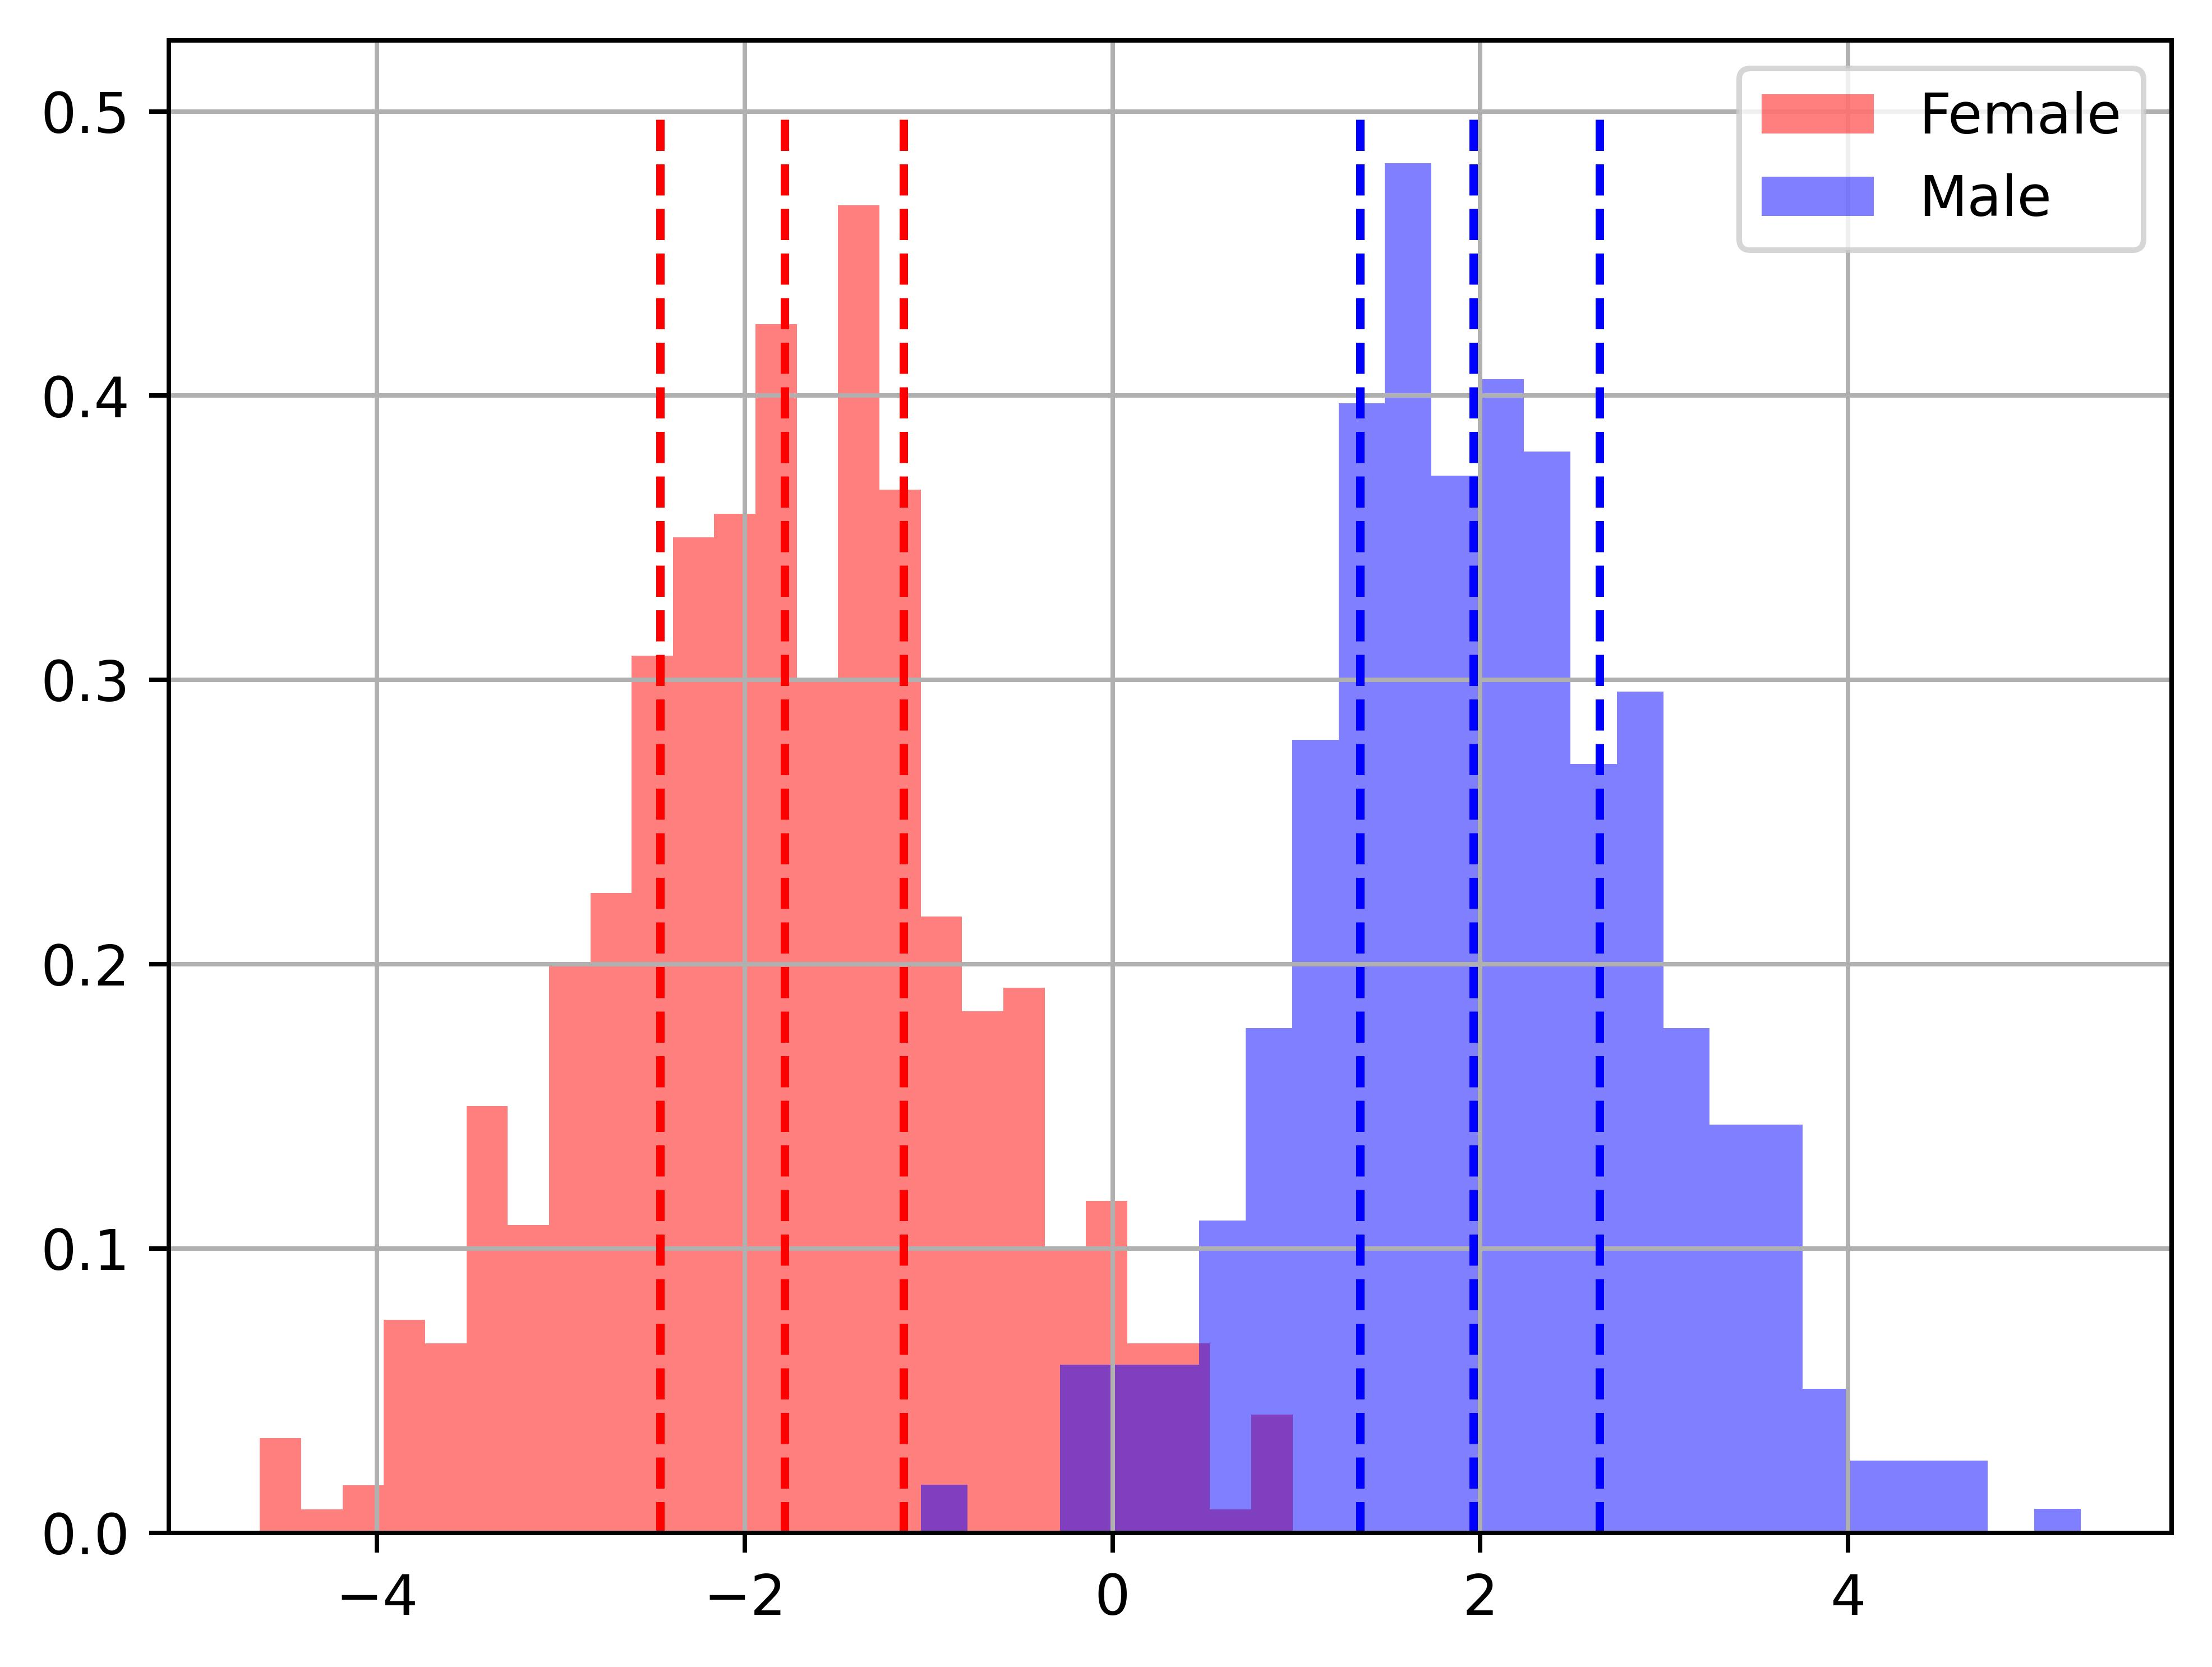
\includegraphics[width=1\textwidth]{../Analysis/LDA/node=15_size=480_step=180_rho=0.1/hist.jpg}
            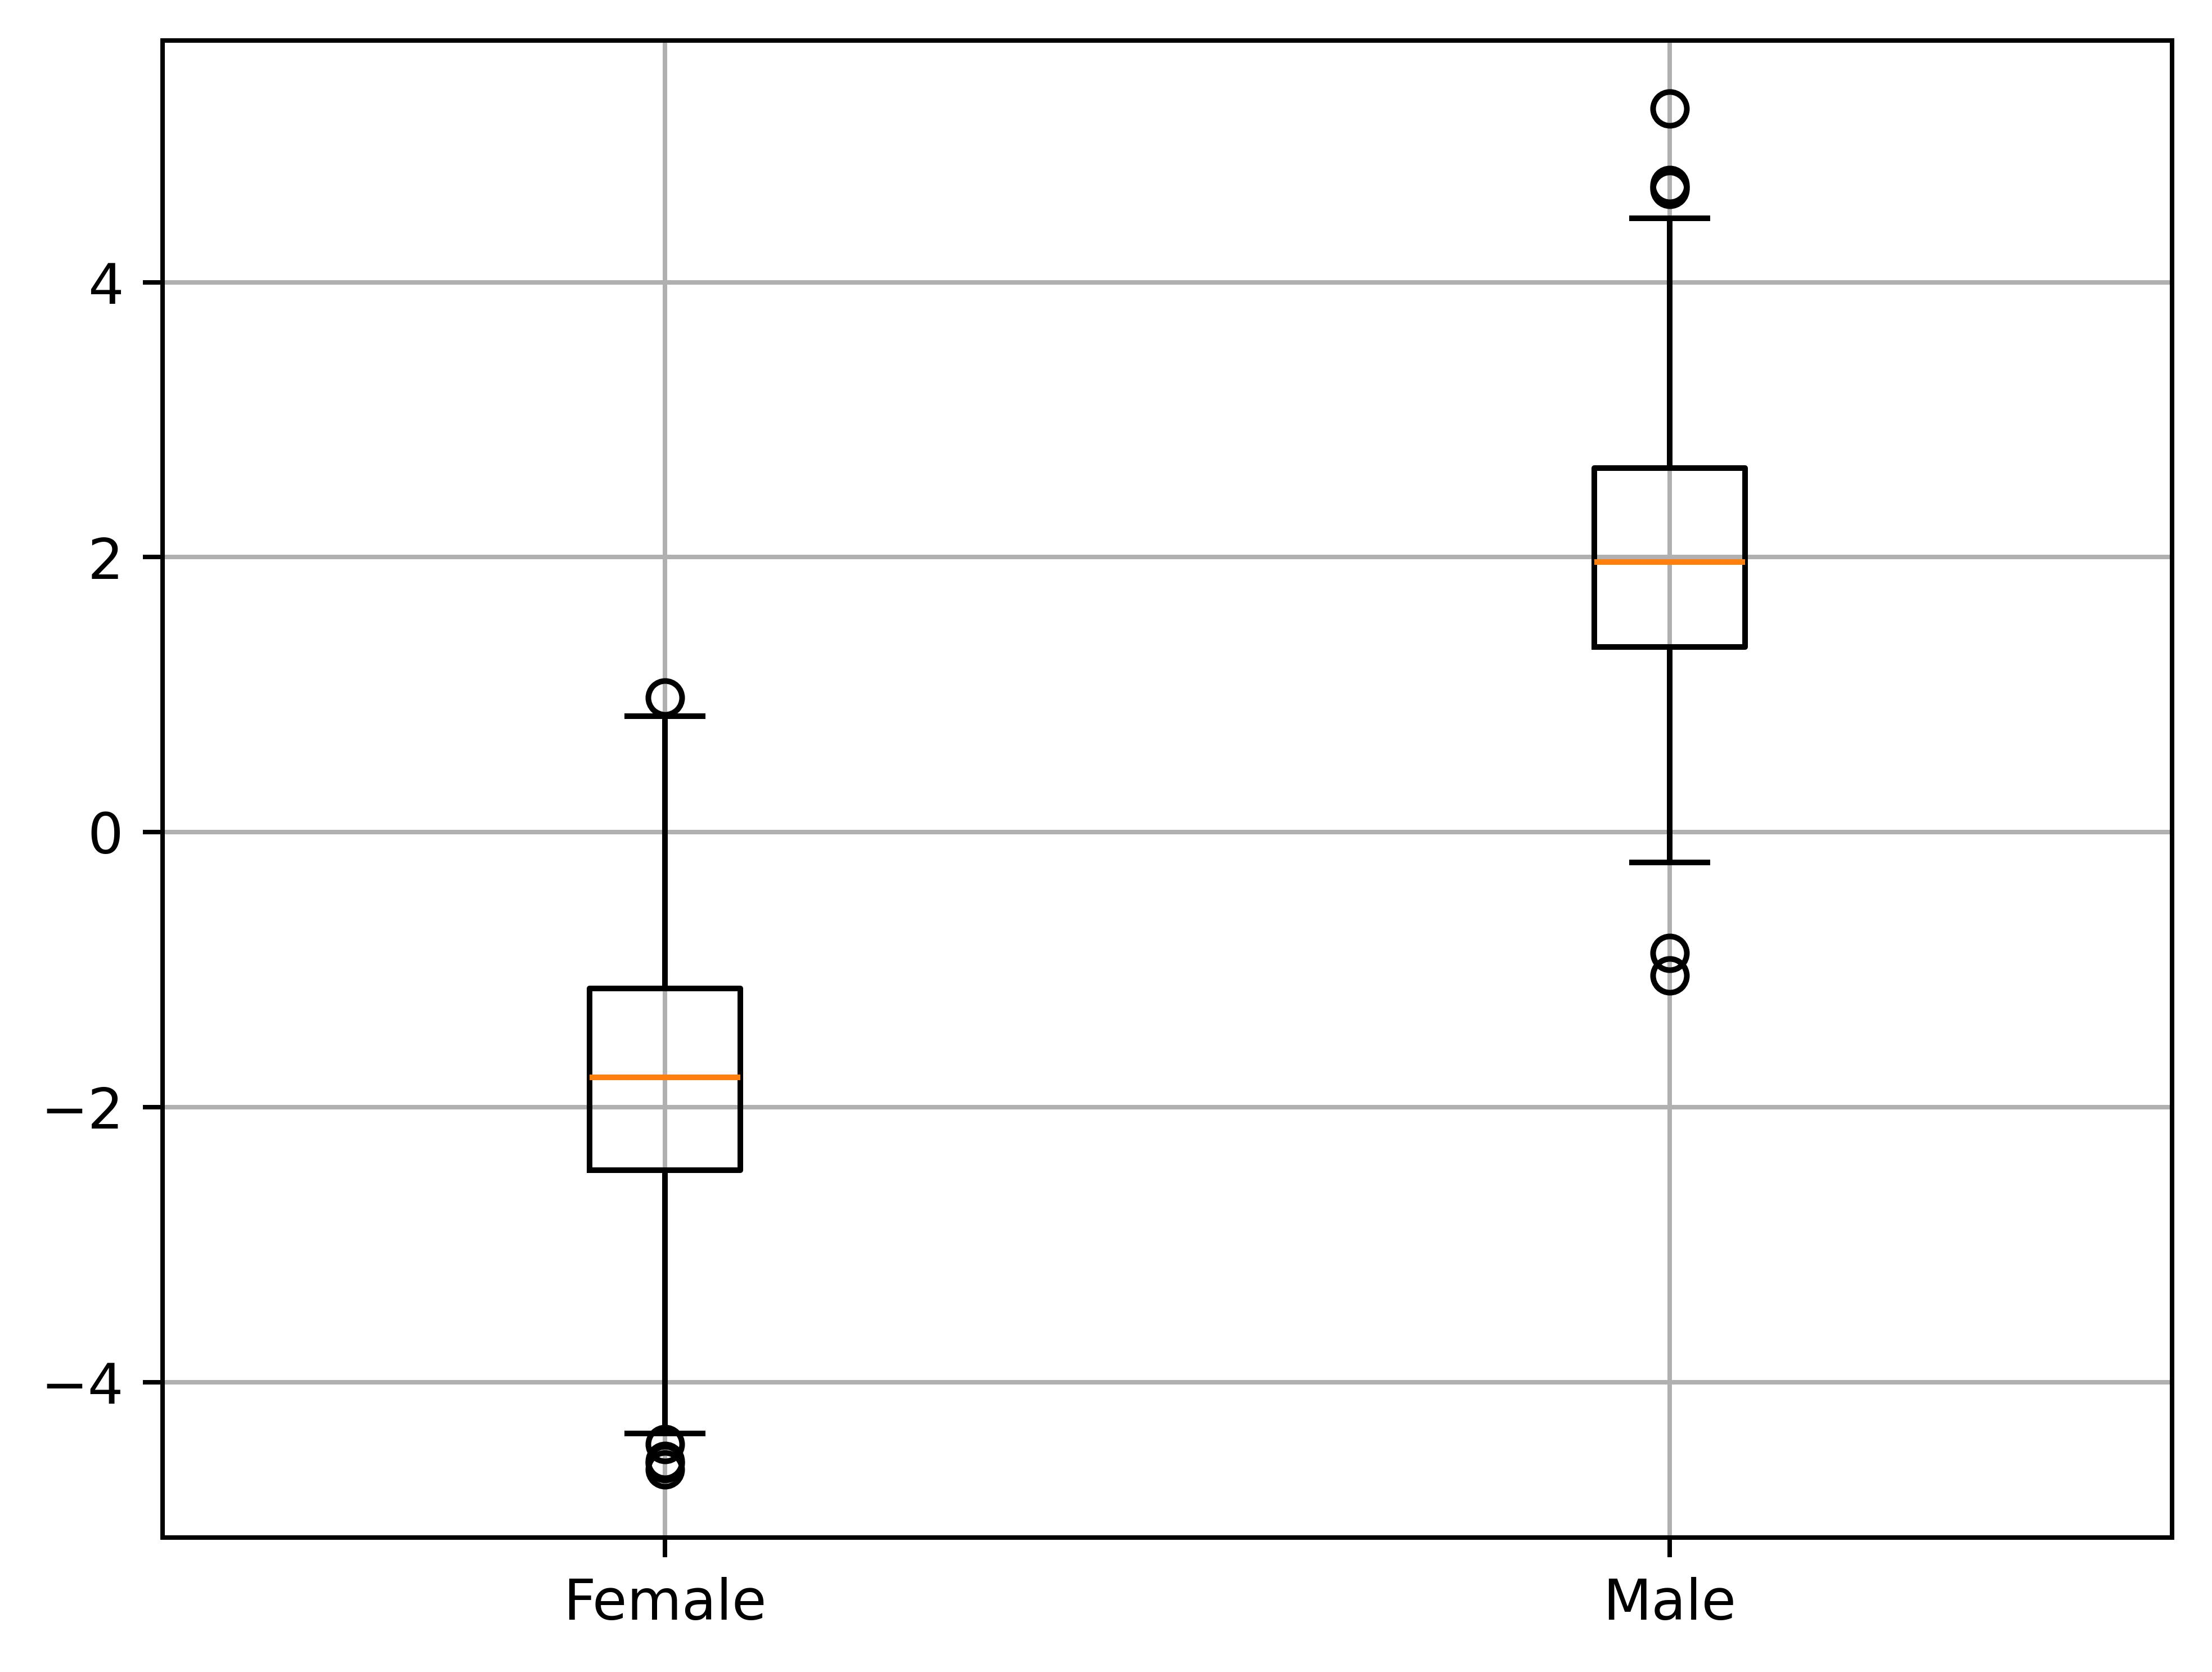
\includegraphics[width=1\textwidth]{../Analysis/LDA/node=15_size=480_step=180_rho=0.1/box.jpg}
        \end{minipage}
    }
    \subfloat[$N_{\text{node}} = 25$]{
        \begin{minipage}[b]{0.3\textwidth}
            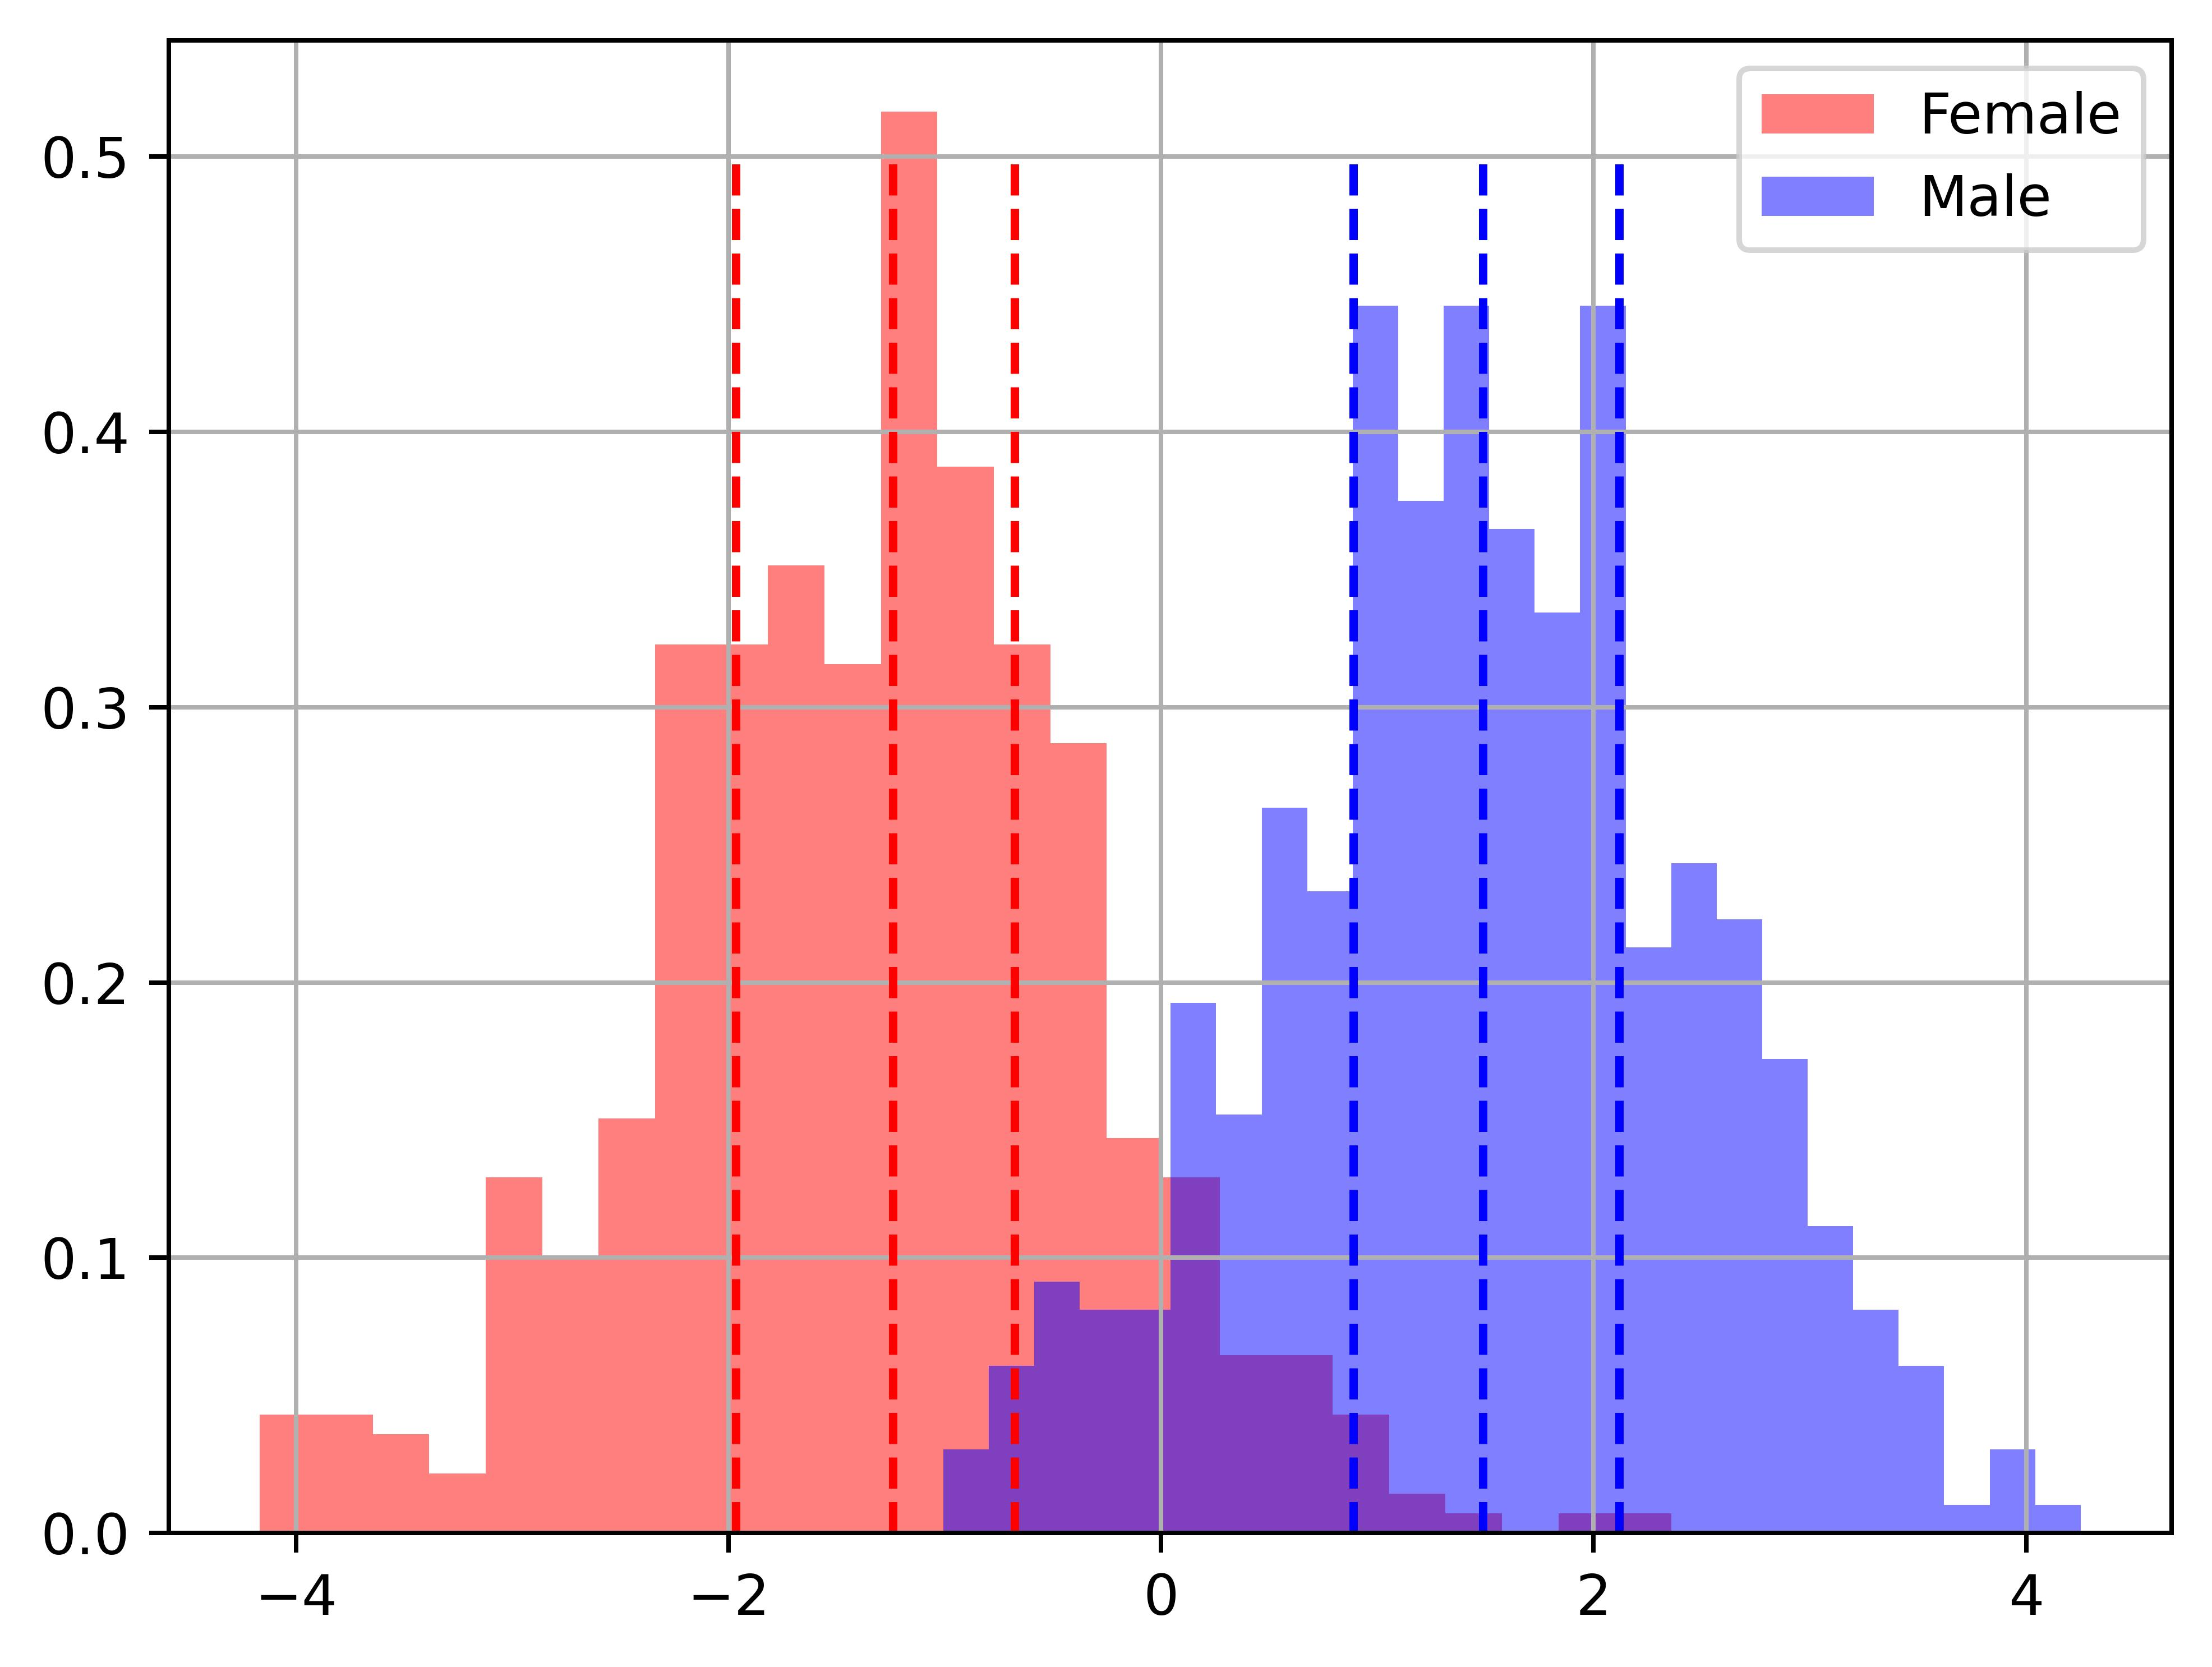
\includegraphics[width=1\textwidth]{../Analysis/LDA/node=25_size=480_step=180_rho=0.1/hist.jpg}
            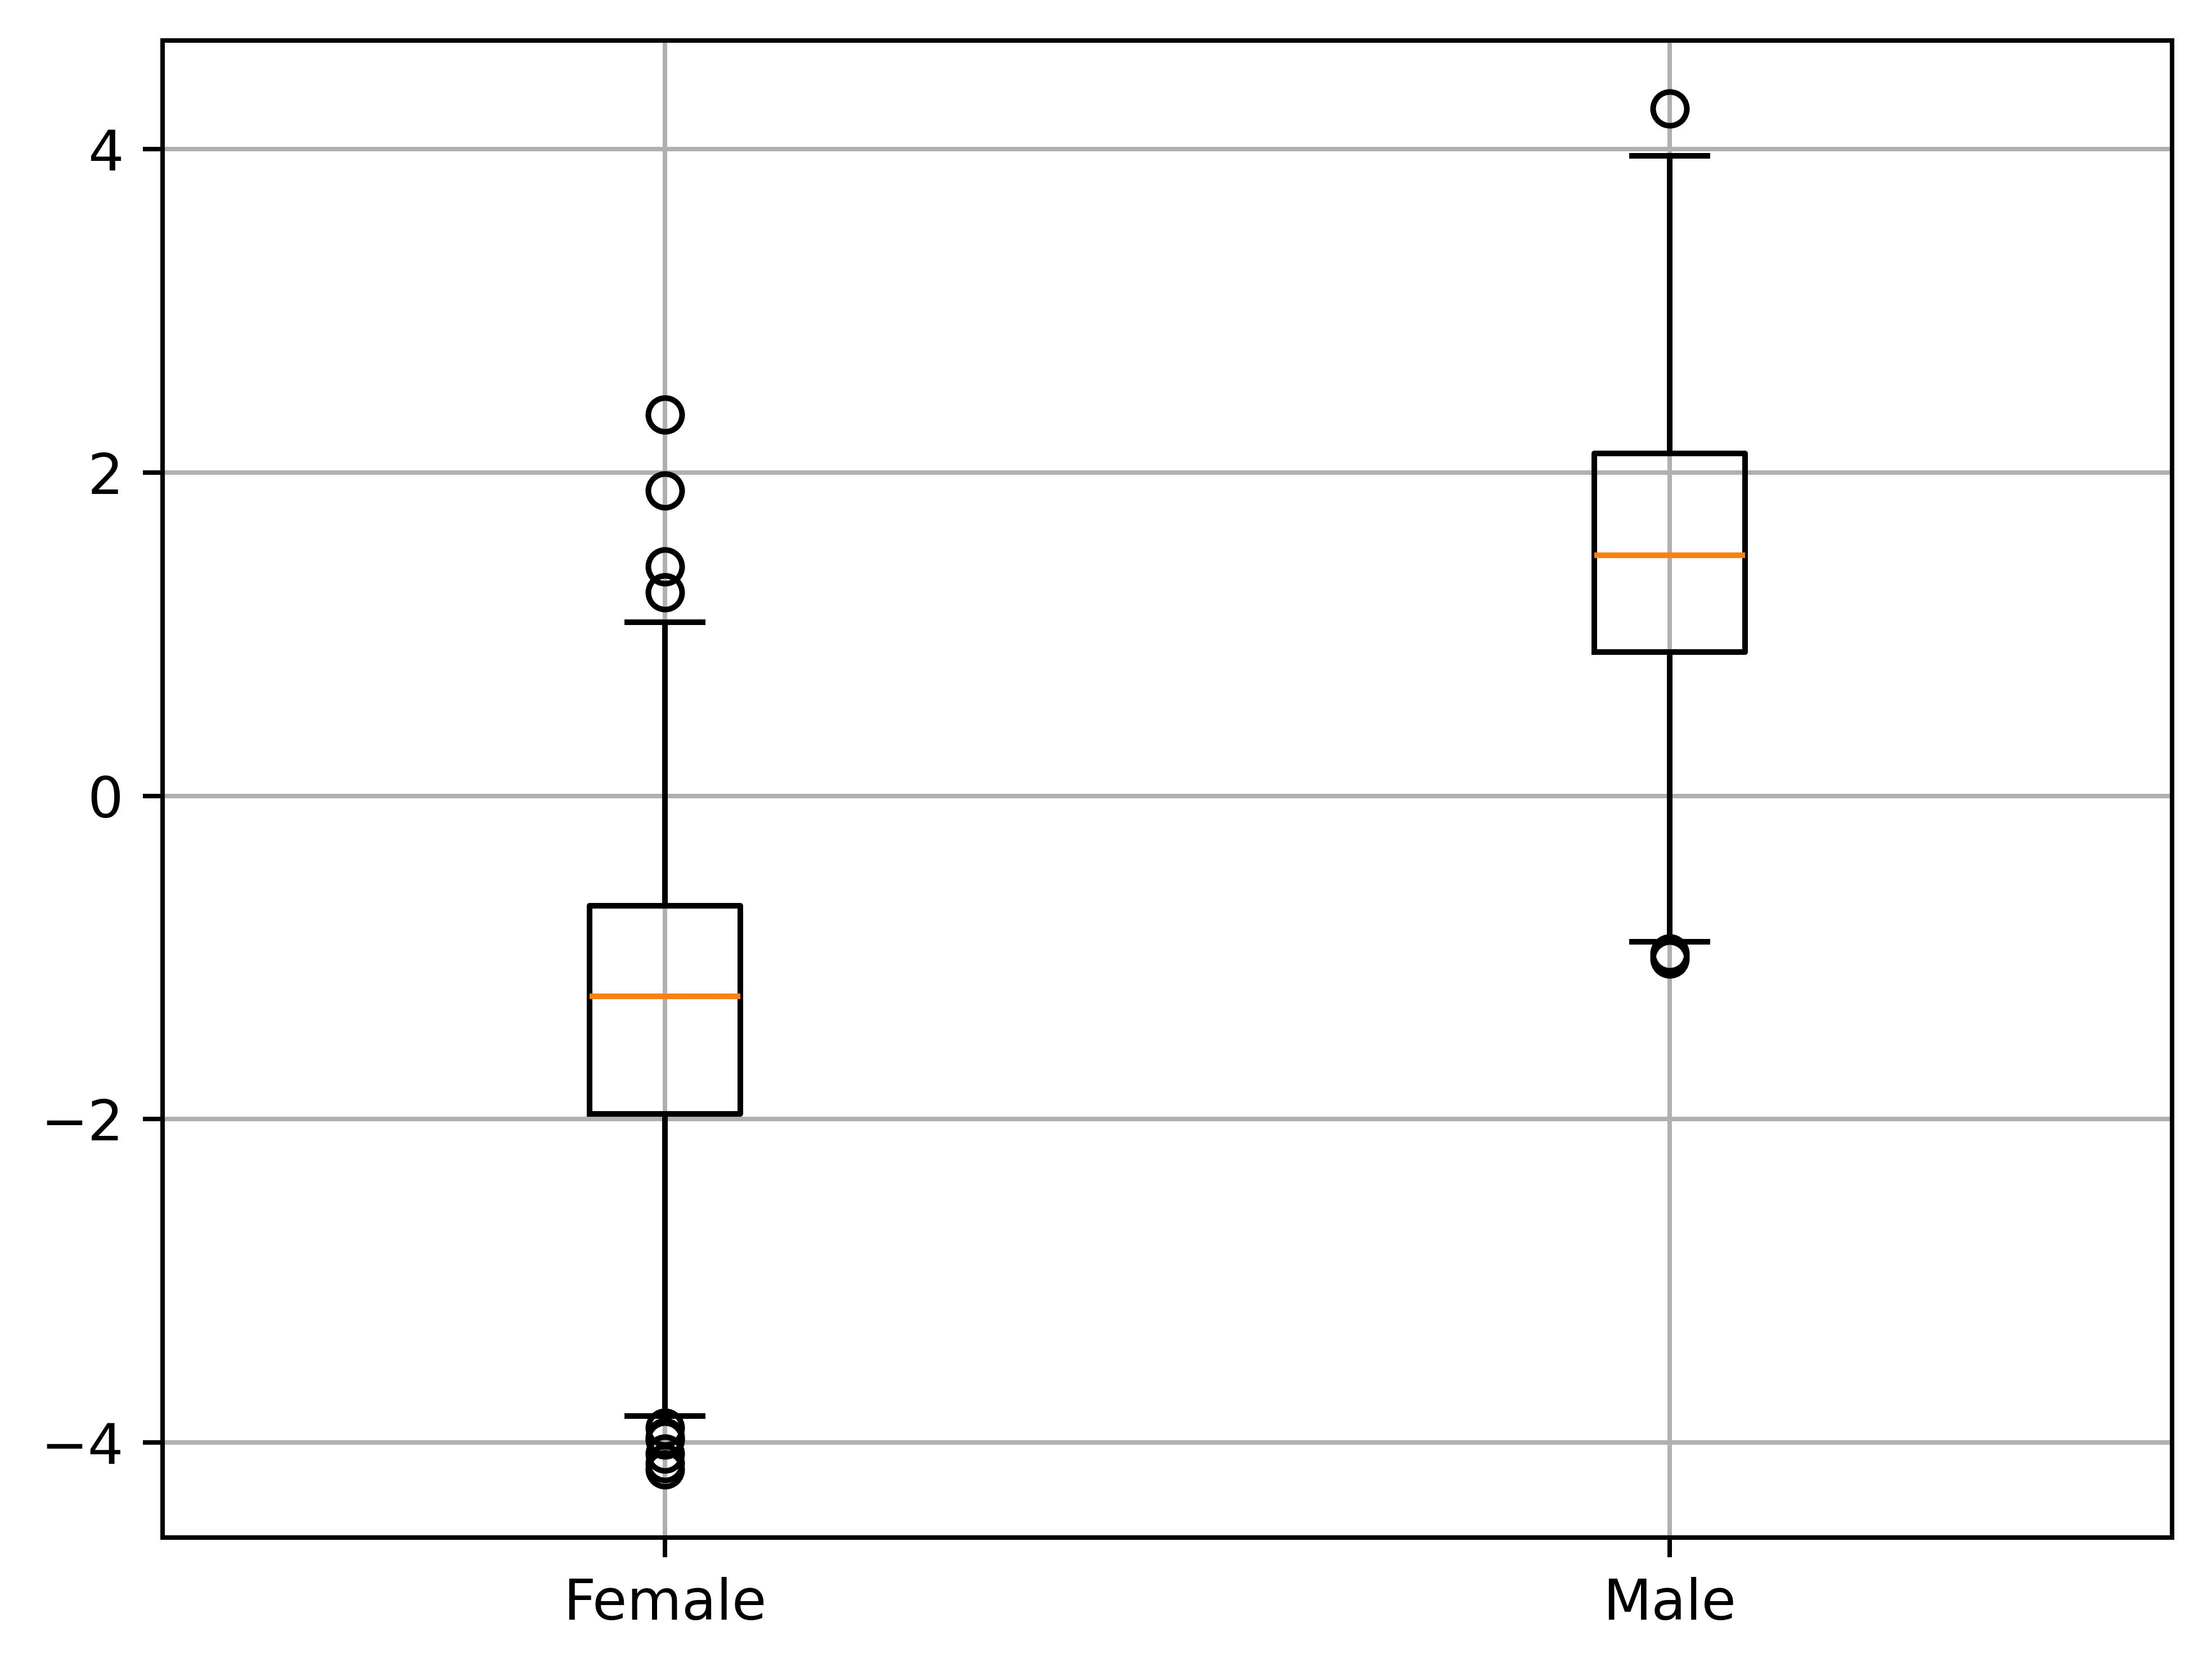
\includegraphics[width=1\textwidth]{../Analysis/LDA/node=25_size=480_step=180_rho=0.1/box.jpg}
        \end{minipage}
    }
    \subfloat[$N_{\text{node}} = 50$]{
        \begin{minipage}[b]{0.3\textwidth}
            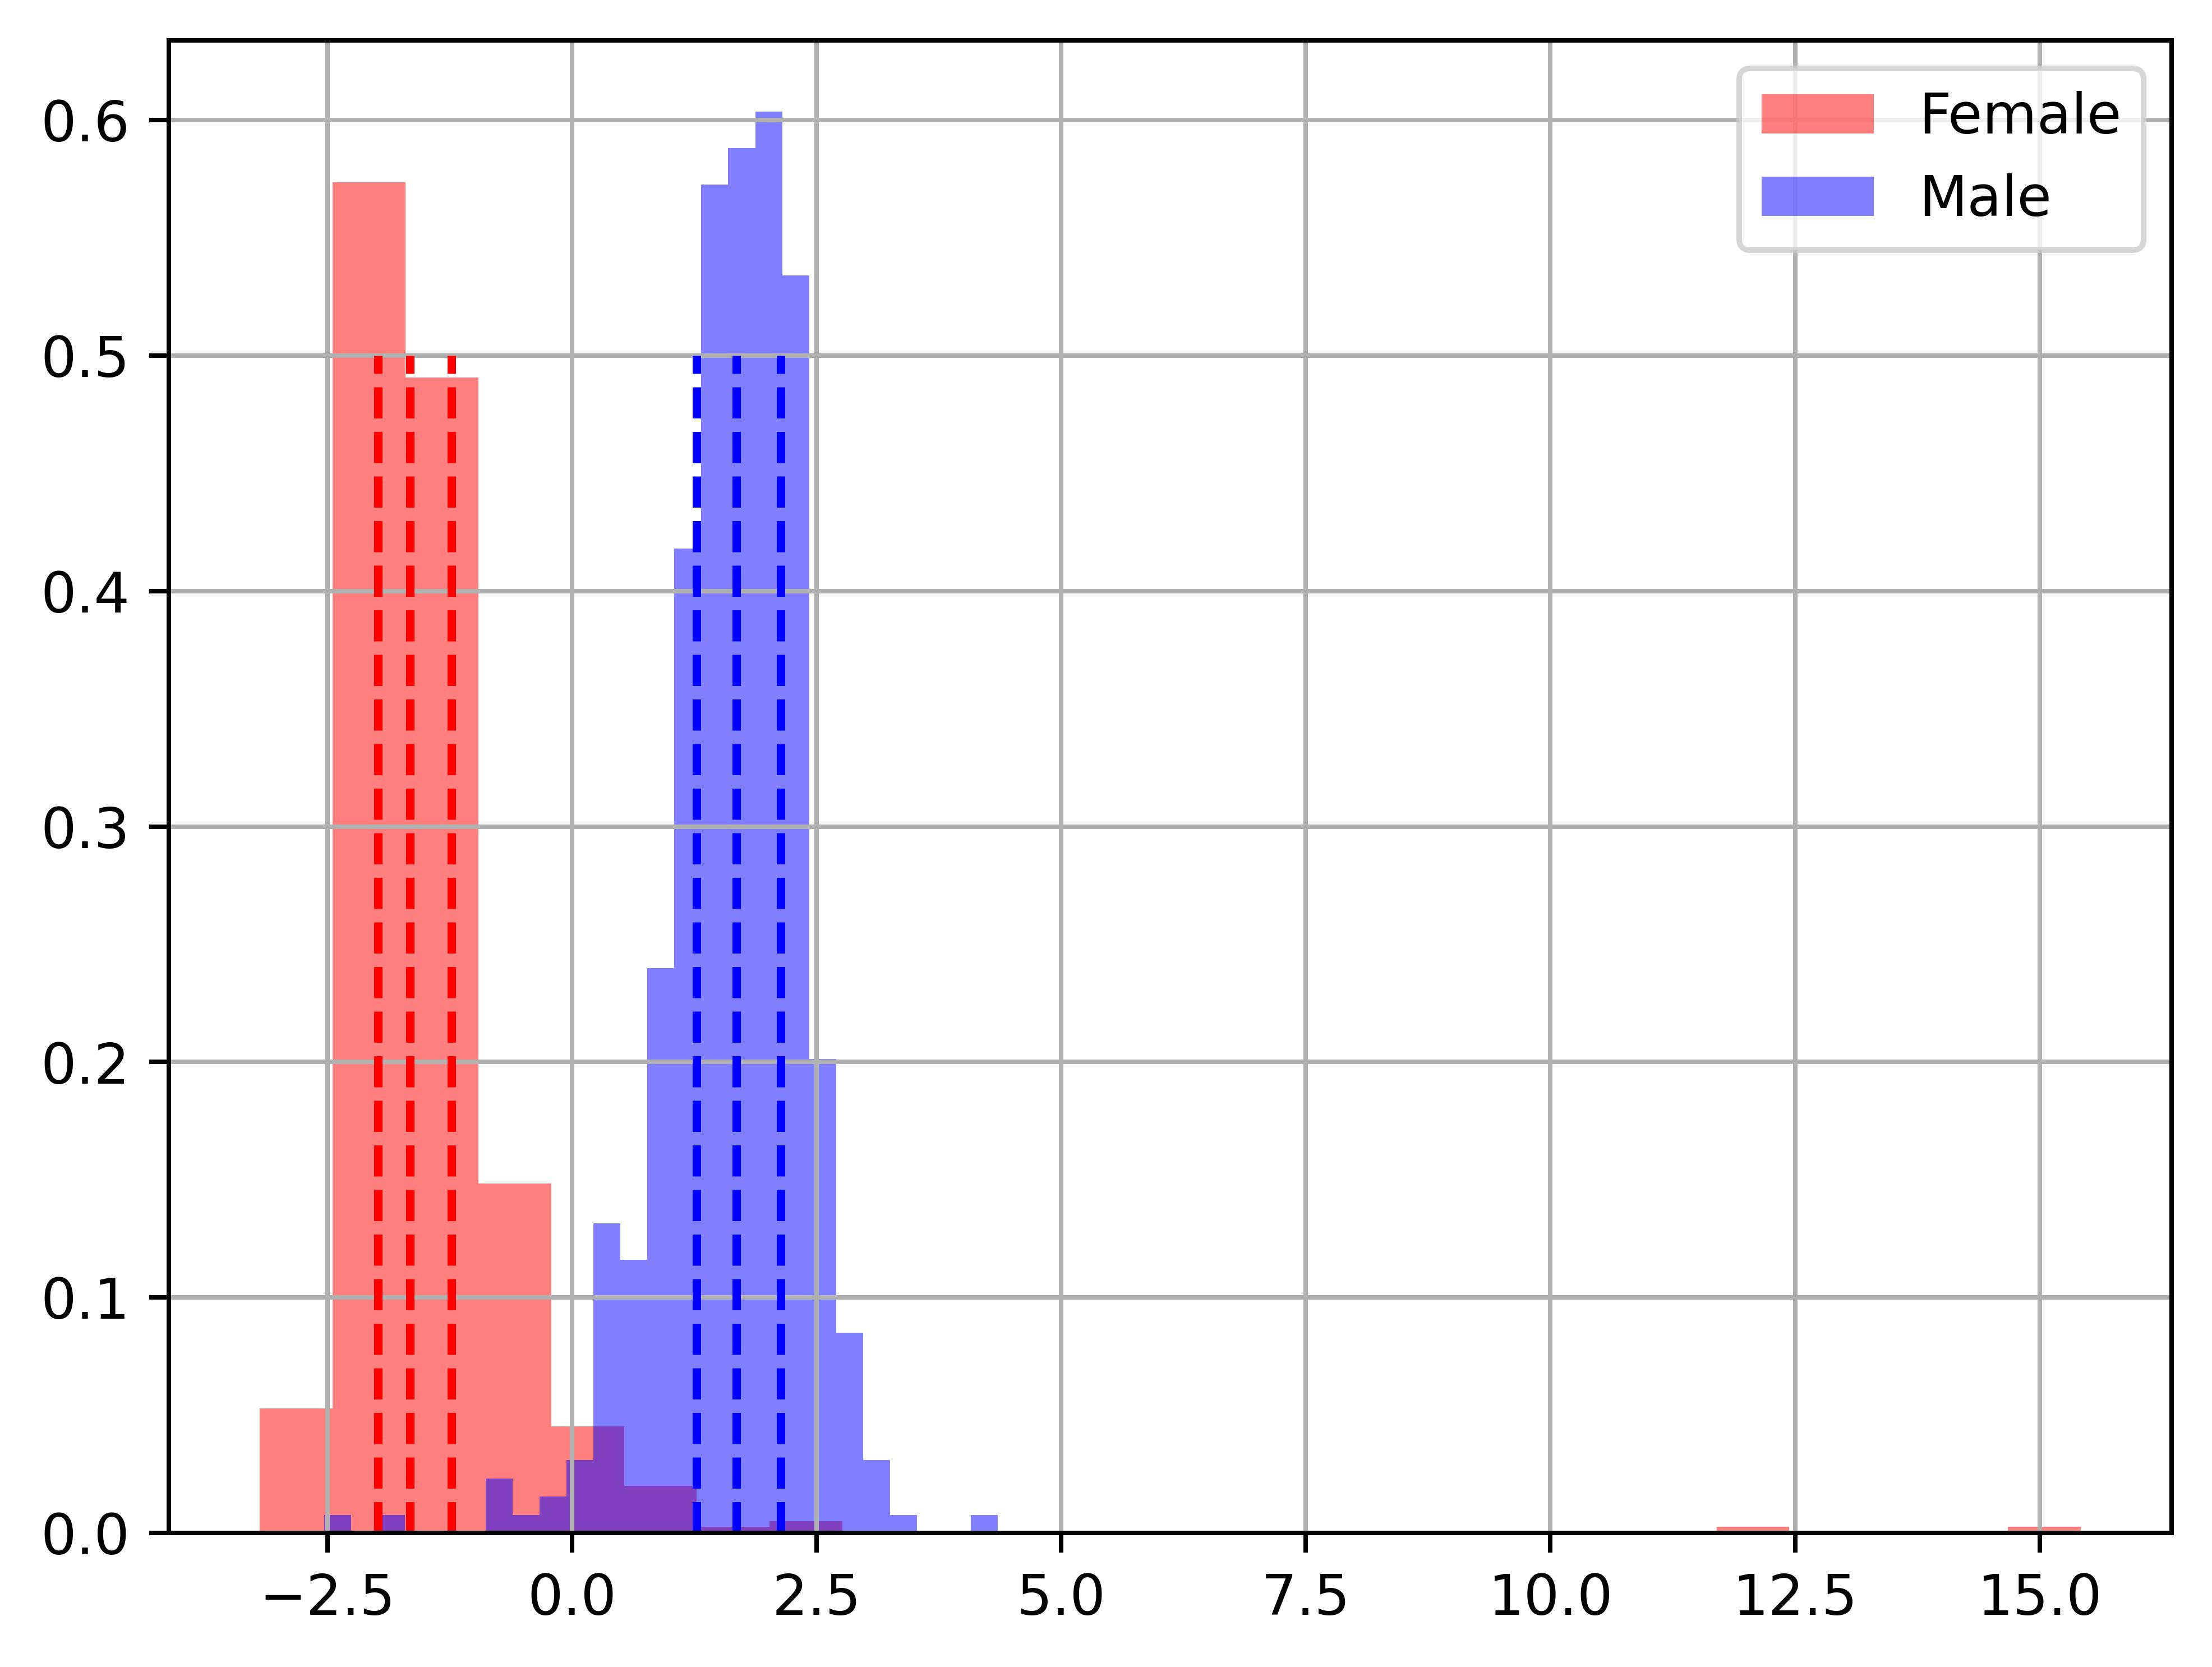
\includegraphics[width=1\textwidth]{../Analysis/LDA/node=50_size=480_step=180_rho=0.1/hist.jpg}
            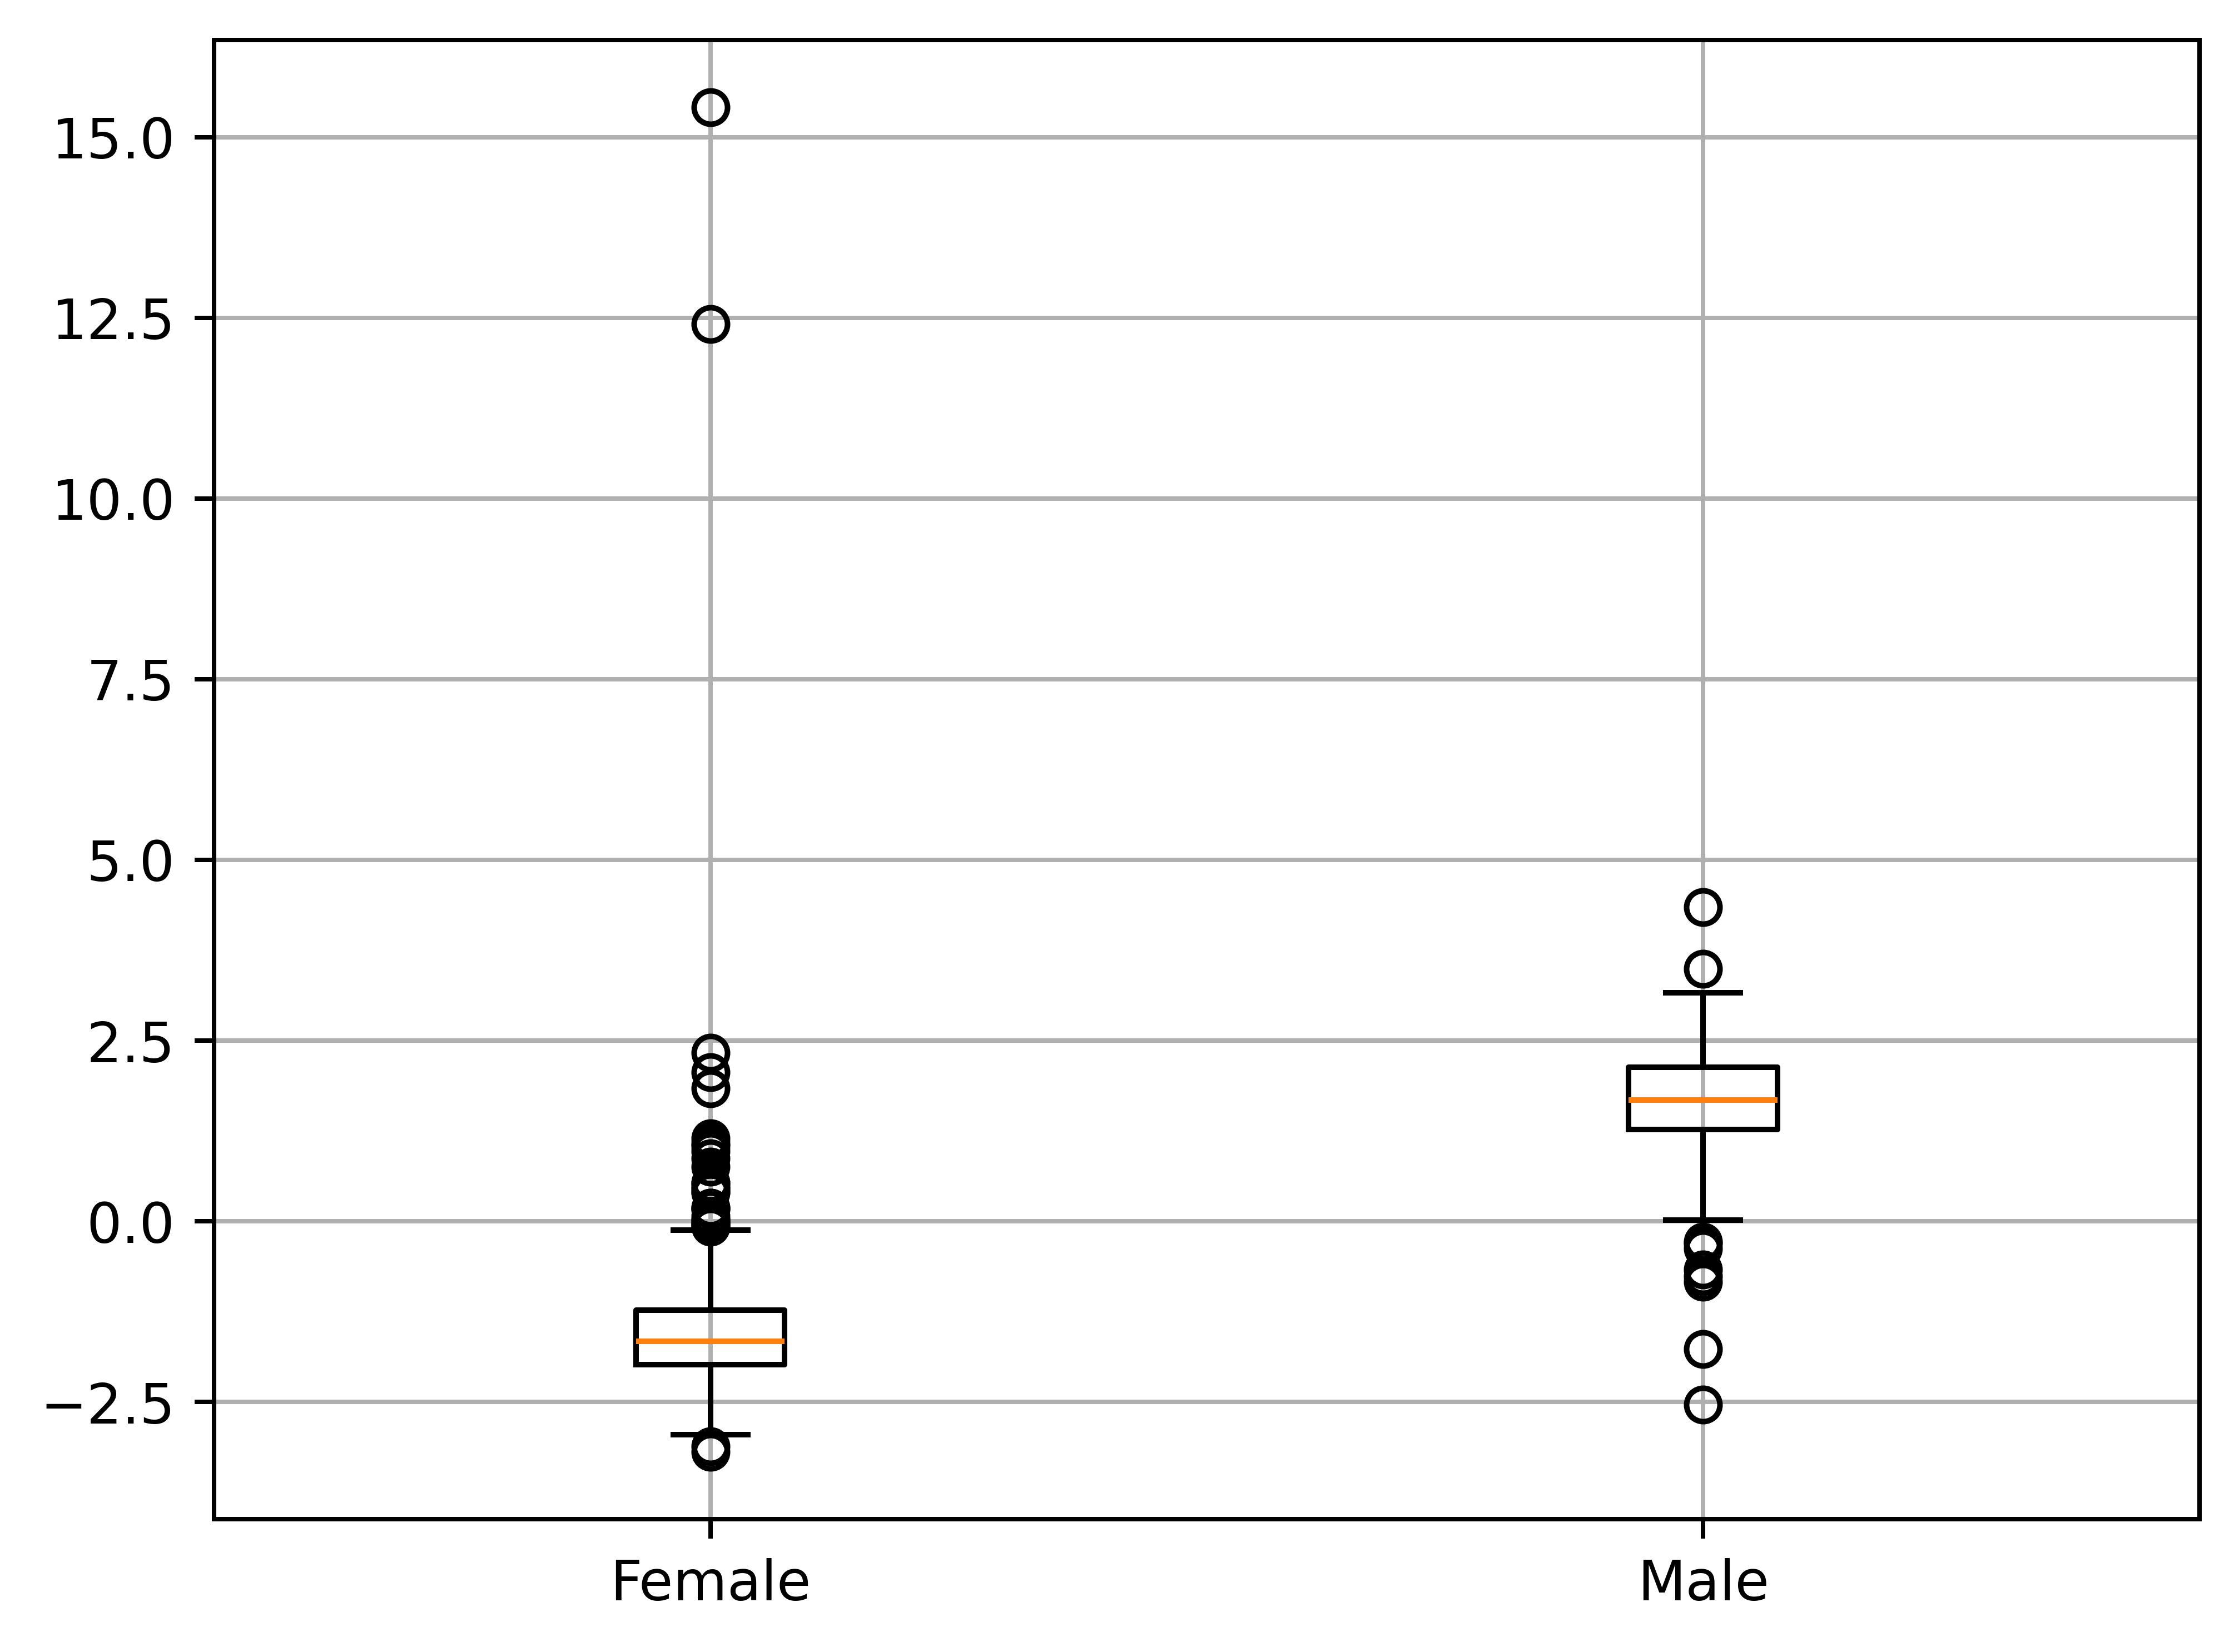
\includegraphics[width=1\textwidth]{../Analysis/LDA/node=50_size=480_step=180_rho=0.1/box.jpg}
        \end{minipage}
    }
    \caption{LDA for dFC.}
    \label{LDA-example-dfc}
\end{figure}

\subsection{Neuroscientific interpretations}

Through the above experiments and analysis, we can find several brain regions with the most significant gender differences. Specifically, denoted by $w_{ij} = w_{ji}$ the weight (particularly, average weight for dFC) for the partial correlation of node $i$ and $j$ given by the models, we sum up the absolute value of the weights for the node $i$, $w_i = \sum_{j=1}^{n} \vert w_{ij} \vert$, which represents how important the region is in the classification. Then the brain regions with corresponding value larger than the threshold will be regard as the most significant regions.

The most significant region for $N_{\text{node}} = 15, 25$ is shown as Figure \ref{msr-n-15} and Figure \ref{msr-n-25}, with the following conclusions: (1) the most significant region of static and dynamic functional connectivity are similar, which means that the differences in these regions are essential in gender classification; (2) the frontal lobe and the parietal lobe are the most significant, meanwhile the diencephalon, the temporal lobe and the occipital lobe also play a important role in gender classification; (3) these region of difference implies that the gender difference may lead to differences in emotion, memory, perception, etc., which is also shows in the previous psychology research\cite{skaalvik1994gender}\cite{soetanto2006there}\cite{wiesenfeld2005sex}\cite{chaplin2013gender}\cite{fischer2018gender}\cite{guillem2005gender}.

\begin{figure}[H]
    \centering
    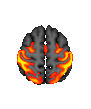
\includegraphics[width=0.2\textwidth]{../Analysis/MIR/groupICA/groupICA_3T_HCP1200_MSMAll_d15.ica/0010.png}
    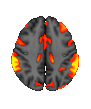
\includegraphics[width=0.2\textwidth]{../Analysis/MIR/groupICA/groupICA_3T_HCP1200_MSMAll_d15.ica/0005.png}
    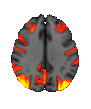
\includegraphics[width=0.2\textwidth]{../Analysis/MIR/groupICA/groupICA_3T_HCP1200_MSMAll_d15.ica/0008.png}
    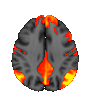
\includegraphics[width=0.2\textwidth]{../Analysis/MIR/groupICA/groupICA_3T_HCP1200_MSMAll_d15.ica/0001.png}
    \caption{The most significant region for $N_{\text{node}} = 15$.}
    \label{msr-n-15}
\end{figure}

\begin{figure}[H]
    \centering
    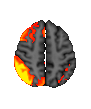
\includegraphics[width=0.2\textwidth]{../Analysis/MIR/groupICA/groupICA_3T_HCP1200_MSMAll_d25.ica/0004.png}
    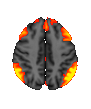
\includegraphics[width=0.2\textwidth]{../Analysis/MIR/groupICA/groupICA_3T_HCP1200_MSMAll_d25.ica/0005.png}
    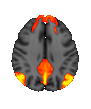
\includegraphics[width=0.2\textwidth]{../Analysis/MIR/groupICA/groupICA_3T_HCP1200_MSMAll_d25.ica/0001.png}
    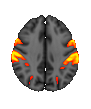
\includegraphics[width=0.2\textwidth]{../Analysis/MIR/groupICA/groupICA_3T_HCP1200_MSMAll_d25.ica/0009.png} \\
    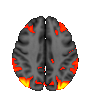
\includegraphics[width=0.2\textwidth]{../Analysis/MIR/groupICA/groupICA_3T_HCP1200_MSMAll_d25.ica/0007.png}
    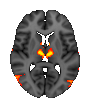
\includegraphics[width=0.2\textwidth]{../Analysis/MIR/groupICA/groupICA_3T_HCP1200_MSMAll_d25.ica/0024.png}
    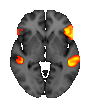
\includegraphics[width=0.2\textwidth]{../Analysis/MIR/groupICA/groupICA_3T_HCP1200_MSMAll_d25.ica/0017.png}
    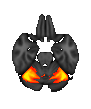
\includegraphics[width=0.2\textwidth]{../Analysis/MIR/groupICA/groupICA_3T_HCP1200_MSMAll_d25.ica/0021.png}
    \caption{The most significant region for $N_{\text{node}} = 25$.}
    \label{msr-n-25}
\end{figure}

\section{Discussion}

In pre-processing step, the choices of size and moving step for sliding windows would make a big difference on the precision of dynamic functional connectivity data that we compute. To be more specific, a shorter window size would lead to better time resolution but poorer frequency resolution, while a wider window size is to the contrary\cite{Leiber2023-de}. Additionally, a larger moving step could reduce the complexity of computation but decrease the detection accuracy\cite{jiang2015flexible}. Consequently, it is important to balance both time and frequency resolution and enhance the capture efficiency of signal characteristics and overall trends for improvement of our experiments in the future. Toward this, employing Fourier analysis\cite{Mantini2007-sv} or wavelet analysis\cite{Medda2016-vh} might work. These 2 methods could analyse complex patterns from time series data with the former decomposing the periodic signal and the latter providing the local features of the signal in the time and frequency domains\cite{Guo2022-dk}.

Additionally, the experimental results for classification with 2 different models training reveal that the AUC of classification is slightly higher with the data trained by CNN than by SVM, while the accuracy rate remains at the same level between the two models. This might be attributed to redundant features extracted by CNN when training data, which means features from different convolutional kernels exhibit convergence.

To address this issue in the future, we might consider to set the coefficients of CNN to be orthogonal. On the one hand,this approach could ensure the unique features extracted from different convolutional kernels and reduce the correlation among features by Orthogonal Projection Loss (OPL)\cite{ranasinghe2021orthogonal}, which offers more significant differences among multiple classes and therefore improves the accuracy of classification. On the other hand, orthogonal initialization could keep the gradients stable during the back-propagation process by maintaining the orthogonality of the weight matrix and therefore alleviate the explosion and vanishing of gradients\cite{Achour2021-rl}, which accelerating the convergence rate of models and increasing the efficiency and performance of training.

Finally, the conclusion that both dynamic and static functional connectivity data are linearly separable bases on the results from 2 linear classifers that we use. But this idea exists some limitations. For example, if the data need to be partitioned to some non-linear target classes, or some complex features of data could not extracted by linear models efficiently. In these conditions, the non-linear classifer such as quadratic classifer would be utilized to partition such data in our future experiments since it could consider the inequality of the in-class covariance matrix and therefore the decision boundary is allowed to take a quadratic form\cite{Rasero2018-hi}, so as to better adapt to the complex structure in the data and partition data with higher efficiency.

\section{Conclusion}

Our results show that there exists gender difference in resting-state functional connectivity, which is linear separable and the accuracy and AUC of linear classifer can reach or even exceed the level of nonlinear classifiers in other papers. The coefficients we obtained also shows that the both for static and dynamic functional connectivity, some of the brain region, such as the frontal lobe and the parietal lobe, are significant in gender classification, which implies that the gender difference may lead to some essential differences in these region, and also the brain functions like emotion, memory, perception, etc..

\newpage

\bibliographystyle{unsrt}
\bibliography{reference.bib}
\addcontentsline{toc}{section}{References}

\newpage

\appendix
\renewcommand\thesection{\Alph{section}}

\section{Supplementary Material}

\subsection{Ablation study for SVM model}

\begin{table}[H]
    \centering
    \begin{tabular}{|c|c|c|c|c|c|}
        \hline
        Method    & Node & Data & min ACC/AUC   & mean ACC/AUC  & max ACC/AUC   \\
        \hline
        LinearSVM & 15   & sFC  & 0.7363/0.7369 & 0.8083/0.8078 & 0.8706/0.8756 \\
        \hline
        LinearSVM & 25   & sFC  & 0.8060/0.8059 & 0.8714/0.8708 & 0.9204/0.9202 \\
        \hline
        LinearSVM & 50   & sFC  & 0.8905/0.8905 & 0.9357/0.9357 & 0.9751/0.9749 \\
        \hline
        LinearSVM & 15   & dFC  & 0.6866/0.6919 & 0.7746/0.7733 & 0.8507/0.8534 \\
        \hline
        LinearSVM & 25   & dFC  & 0.7861/0.7874 & 0.8739/0.8730 & 0.9204/0.9206 \\
        \hline
        LinearSVM & 50   & dFC  & 0.8806/0.8813 & 0.9295/0.9300 & 0.9652/0.9666 \\
        \hline
        Nu-SVM    & 15   & sFC  & 0.7562/0.7571 & 0.8221/0.8219 & 0.8856/0.8847 \\
        \hline
        Nu-SVM    & 25   & sFC  & 0.8259/0.8257 & 0.8791/0.8782 & 0.9303/0.9302 \\
        \hline
        Nu-SVM    & 50   & sFC  & 0.8458/0.8458 & 0.9191/0.9194 & 0.9602/0.9608 \\
        \hline
        Nu-SVM    & 15   & dFC  & 0.7313/0.7324 & 0.8066/0.8056 & 0.8706/0.8674 \\
        \hline
        Nu-SVM    & 25   & dFC  & 0.8109/0.8121 & 0.8811/0.8802 & 0.9303/0.9296 \\
        \hline
        Nu-SVM    & 50   & dFC  & 0.8308/0.8300 & 0.9021/0.9022 & 0.9552/0.9579 \\
        \hline
    \end{tabular}
    \caption{Ablation study for SVM.}
\end{table}

\begin{figure}[H]
    \centering
    \subfloat[test ACC for LinearSVM]{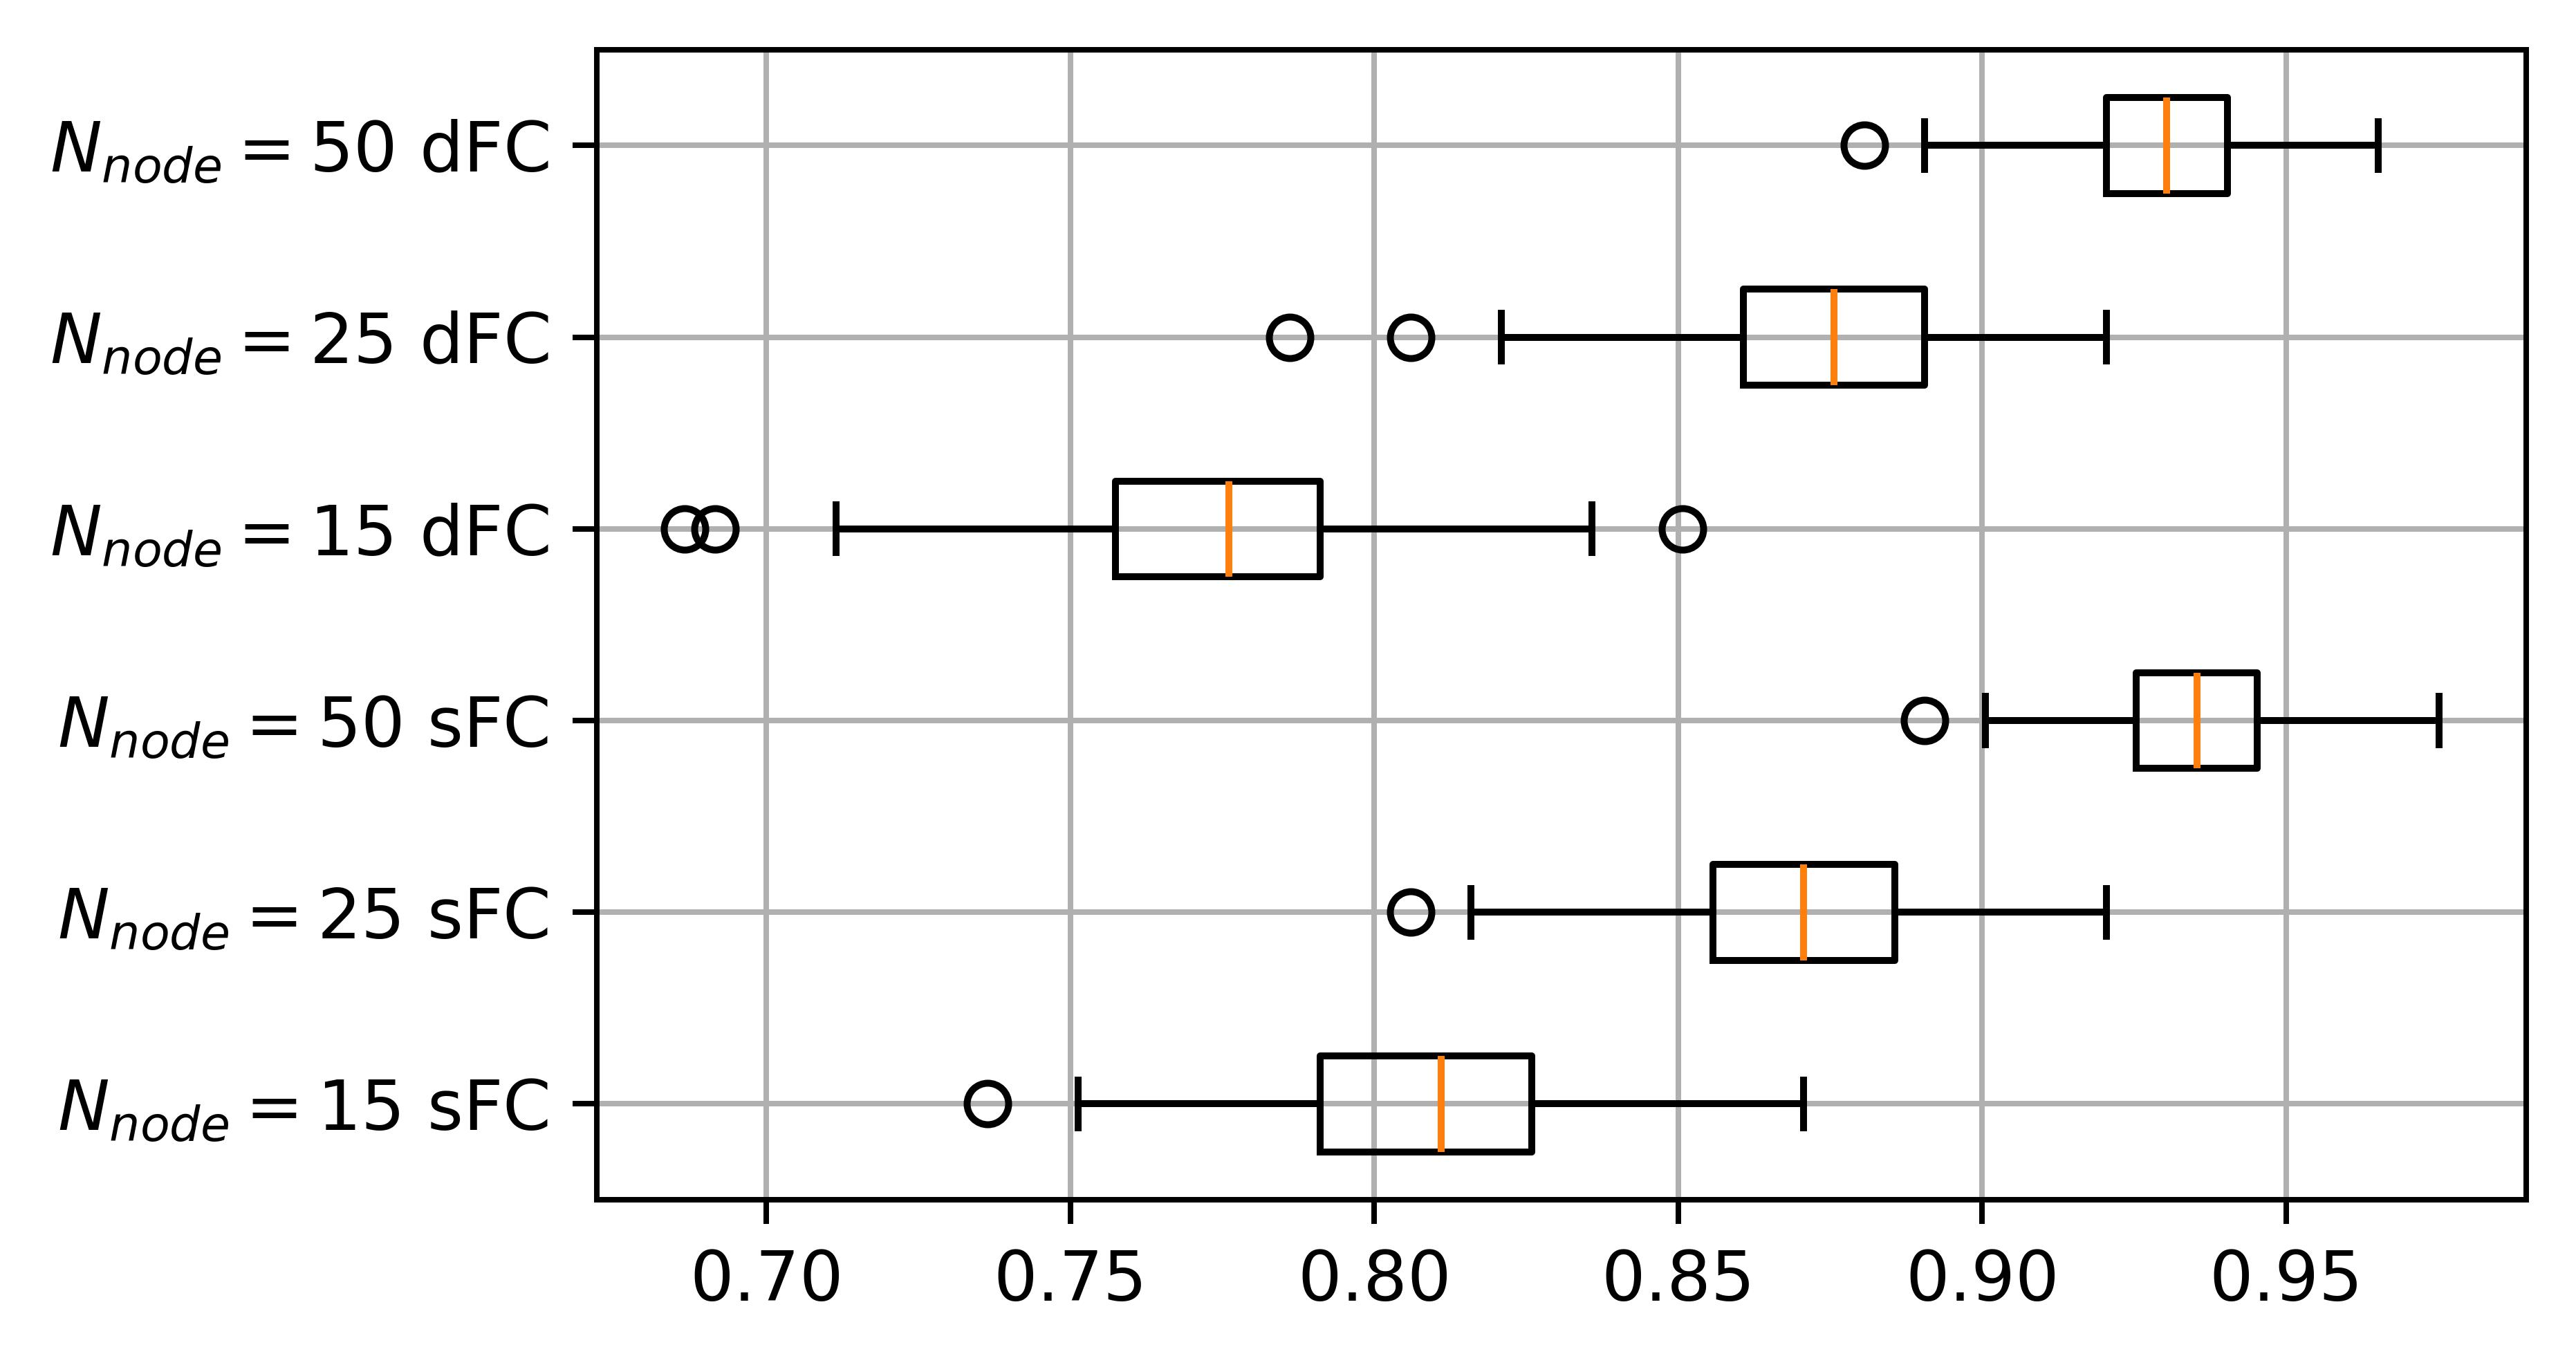
\includegraphics[width=0.4\textwidth]{../SVM/acc_linear_0.1.jpg}}
    \subfloat[test AUC for LinearSVM]{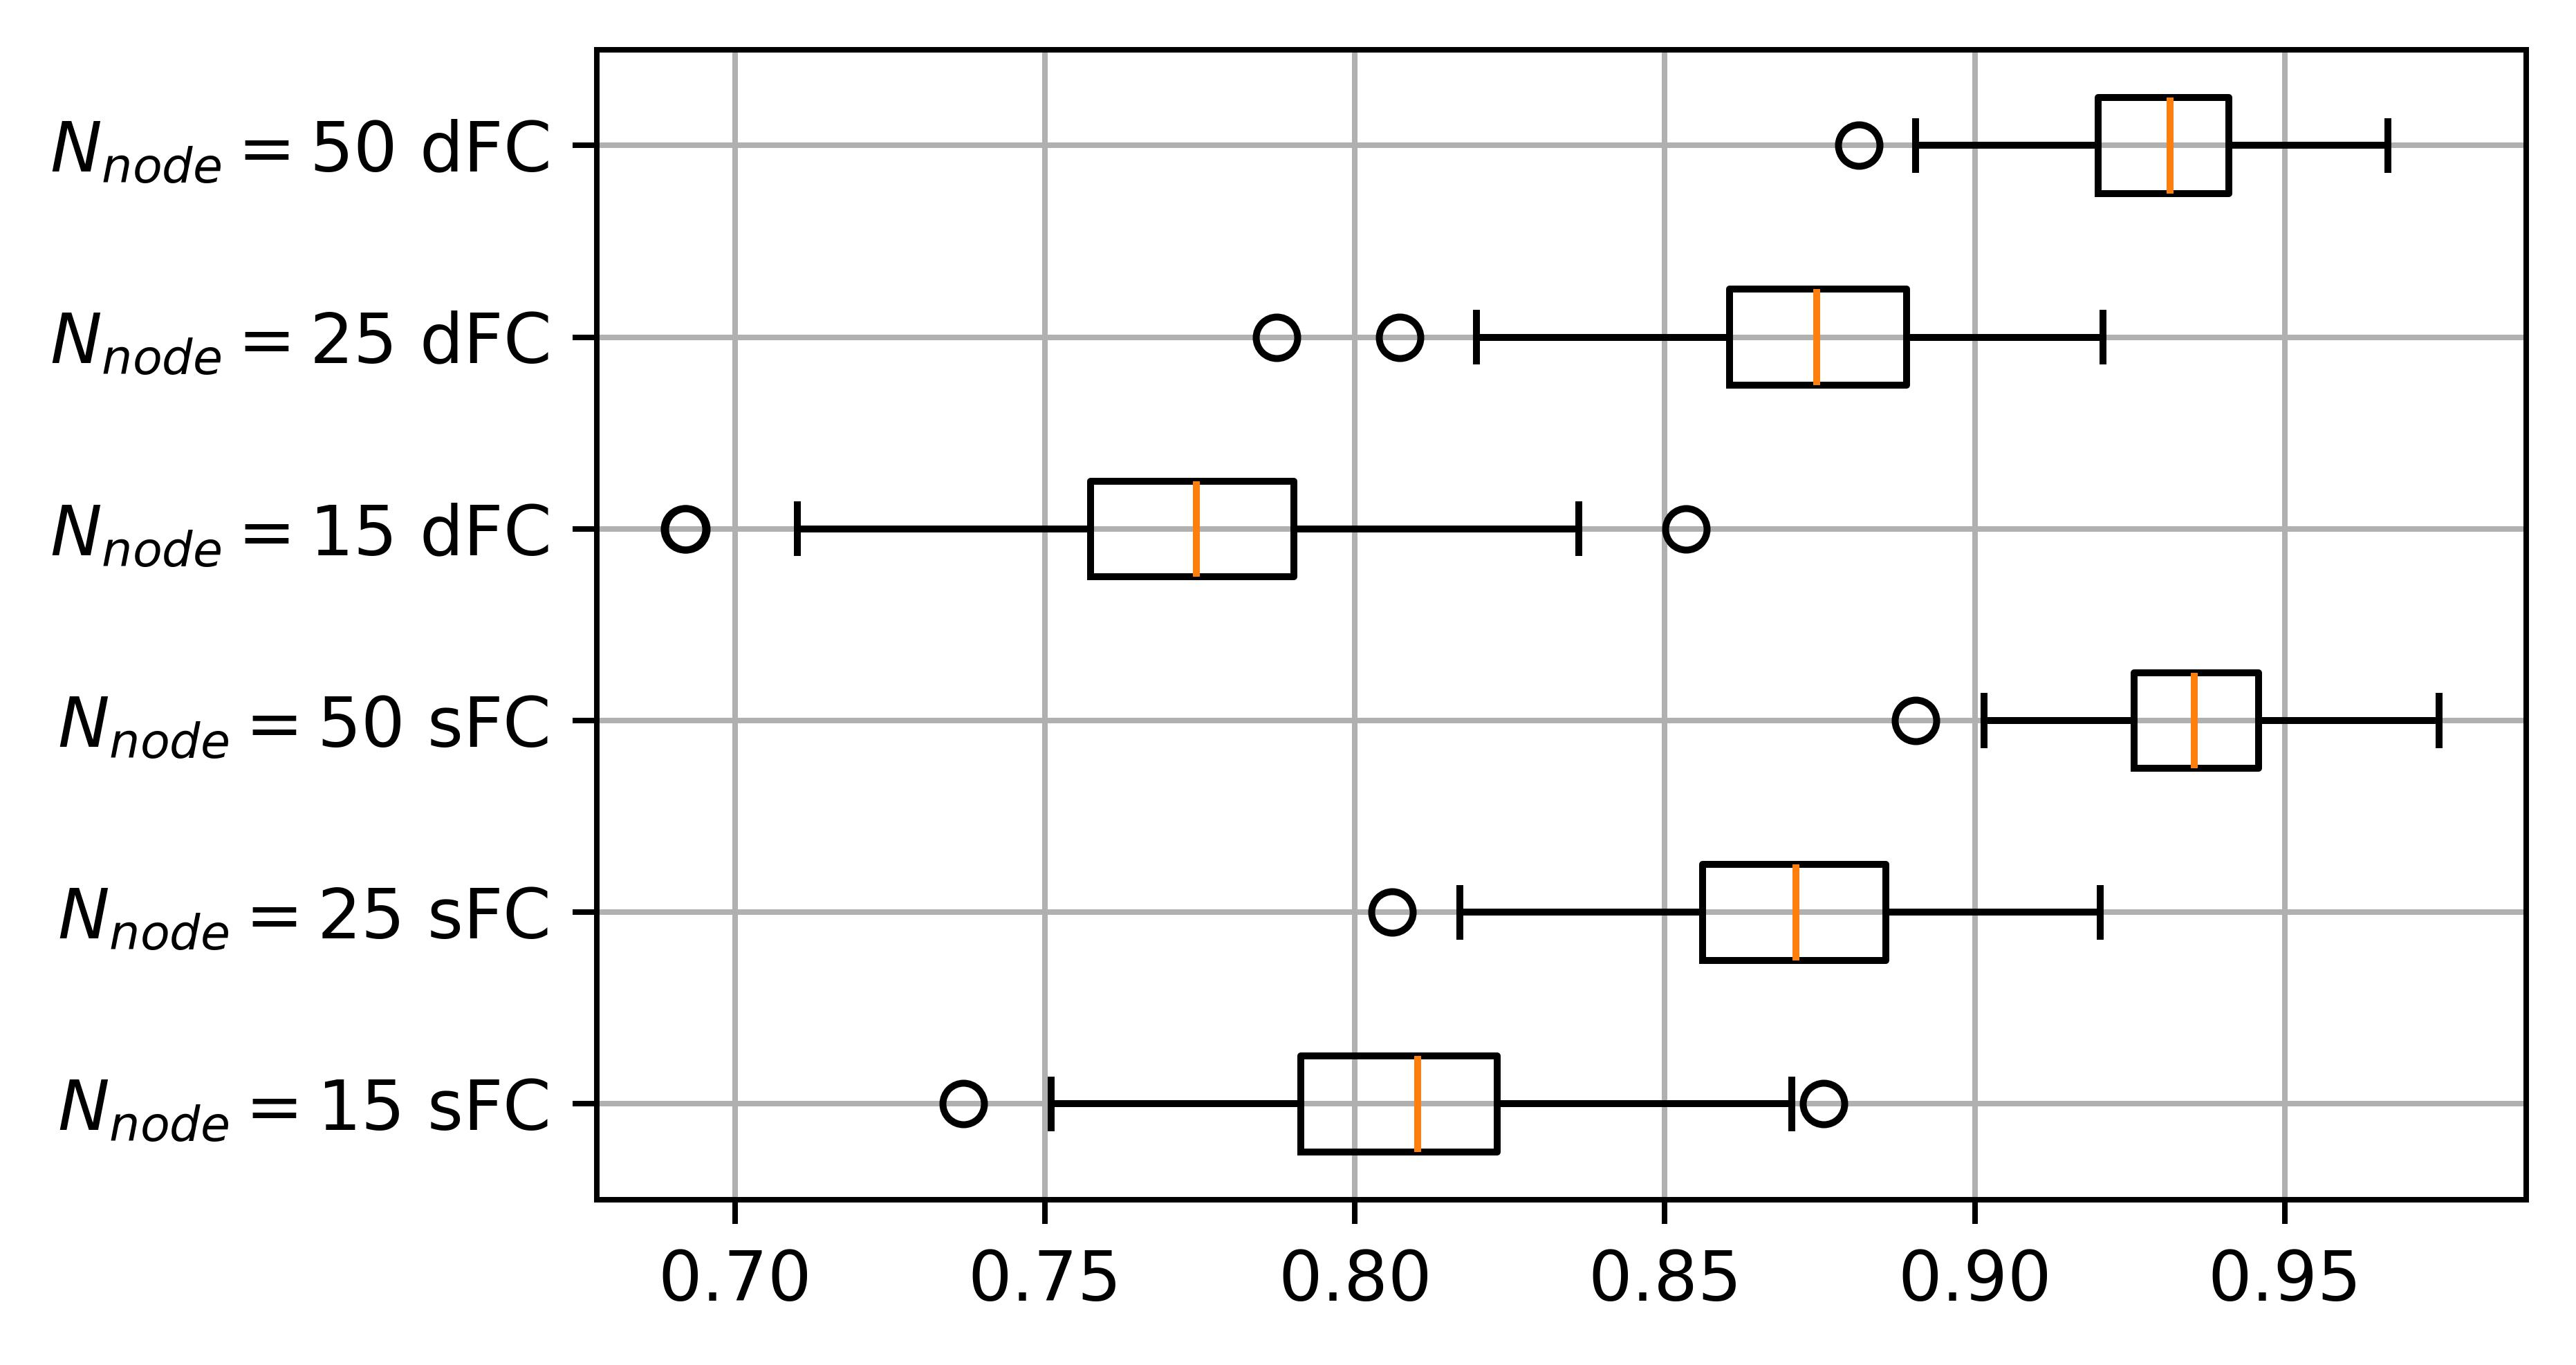
\includegraphics[width=0.4\textwidth]{../SVM/auc_linear_0.1.jpg}} \\
    \subfloat[test ACC for NuSVM]{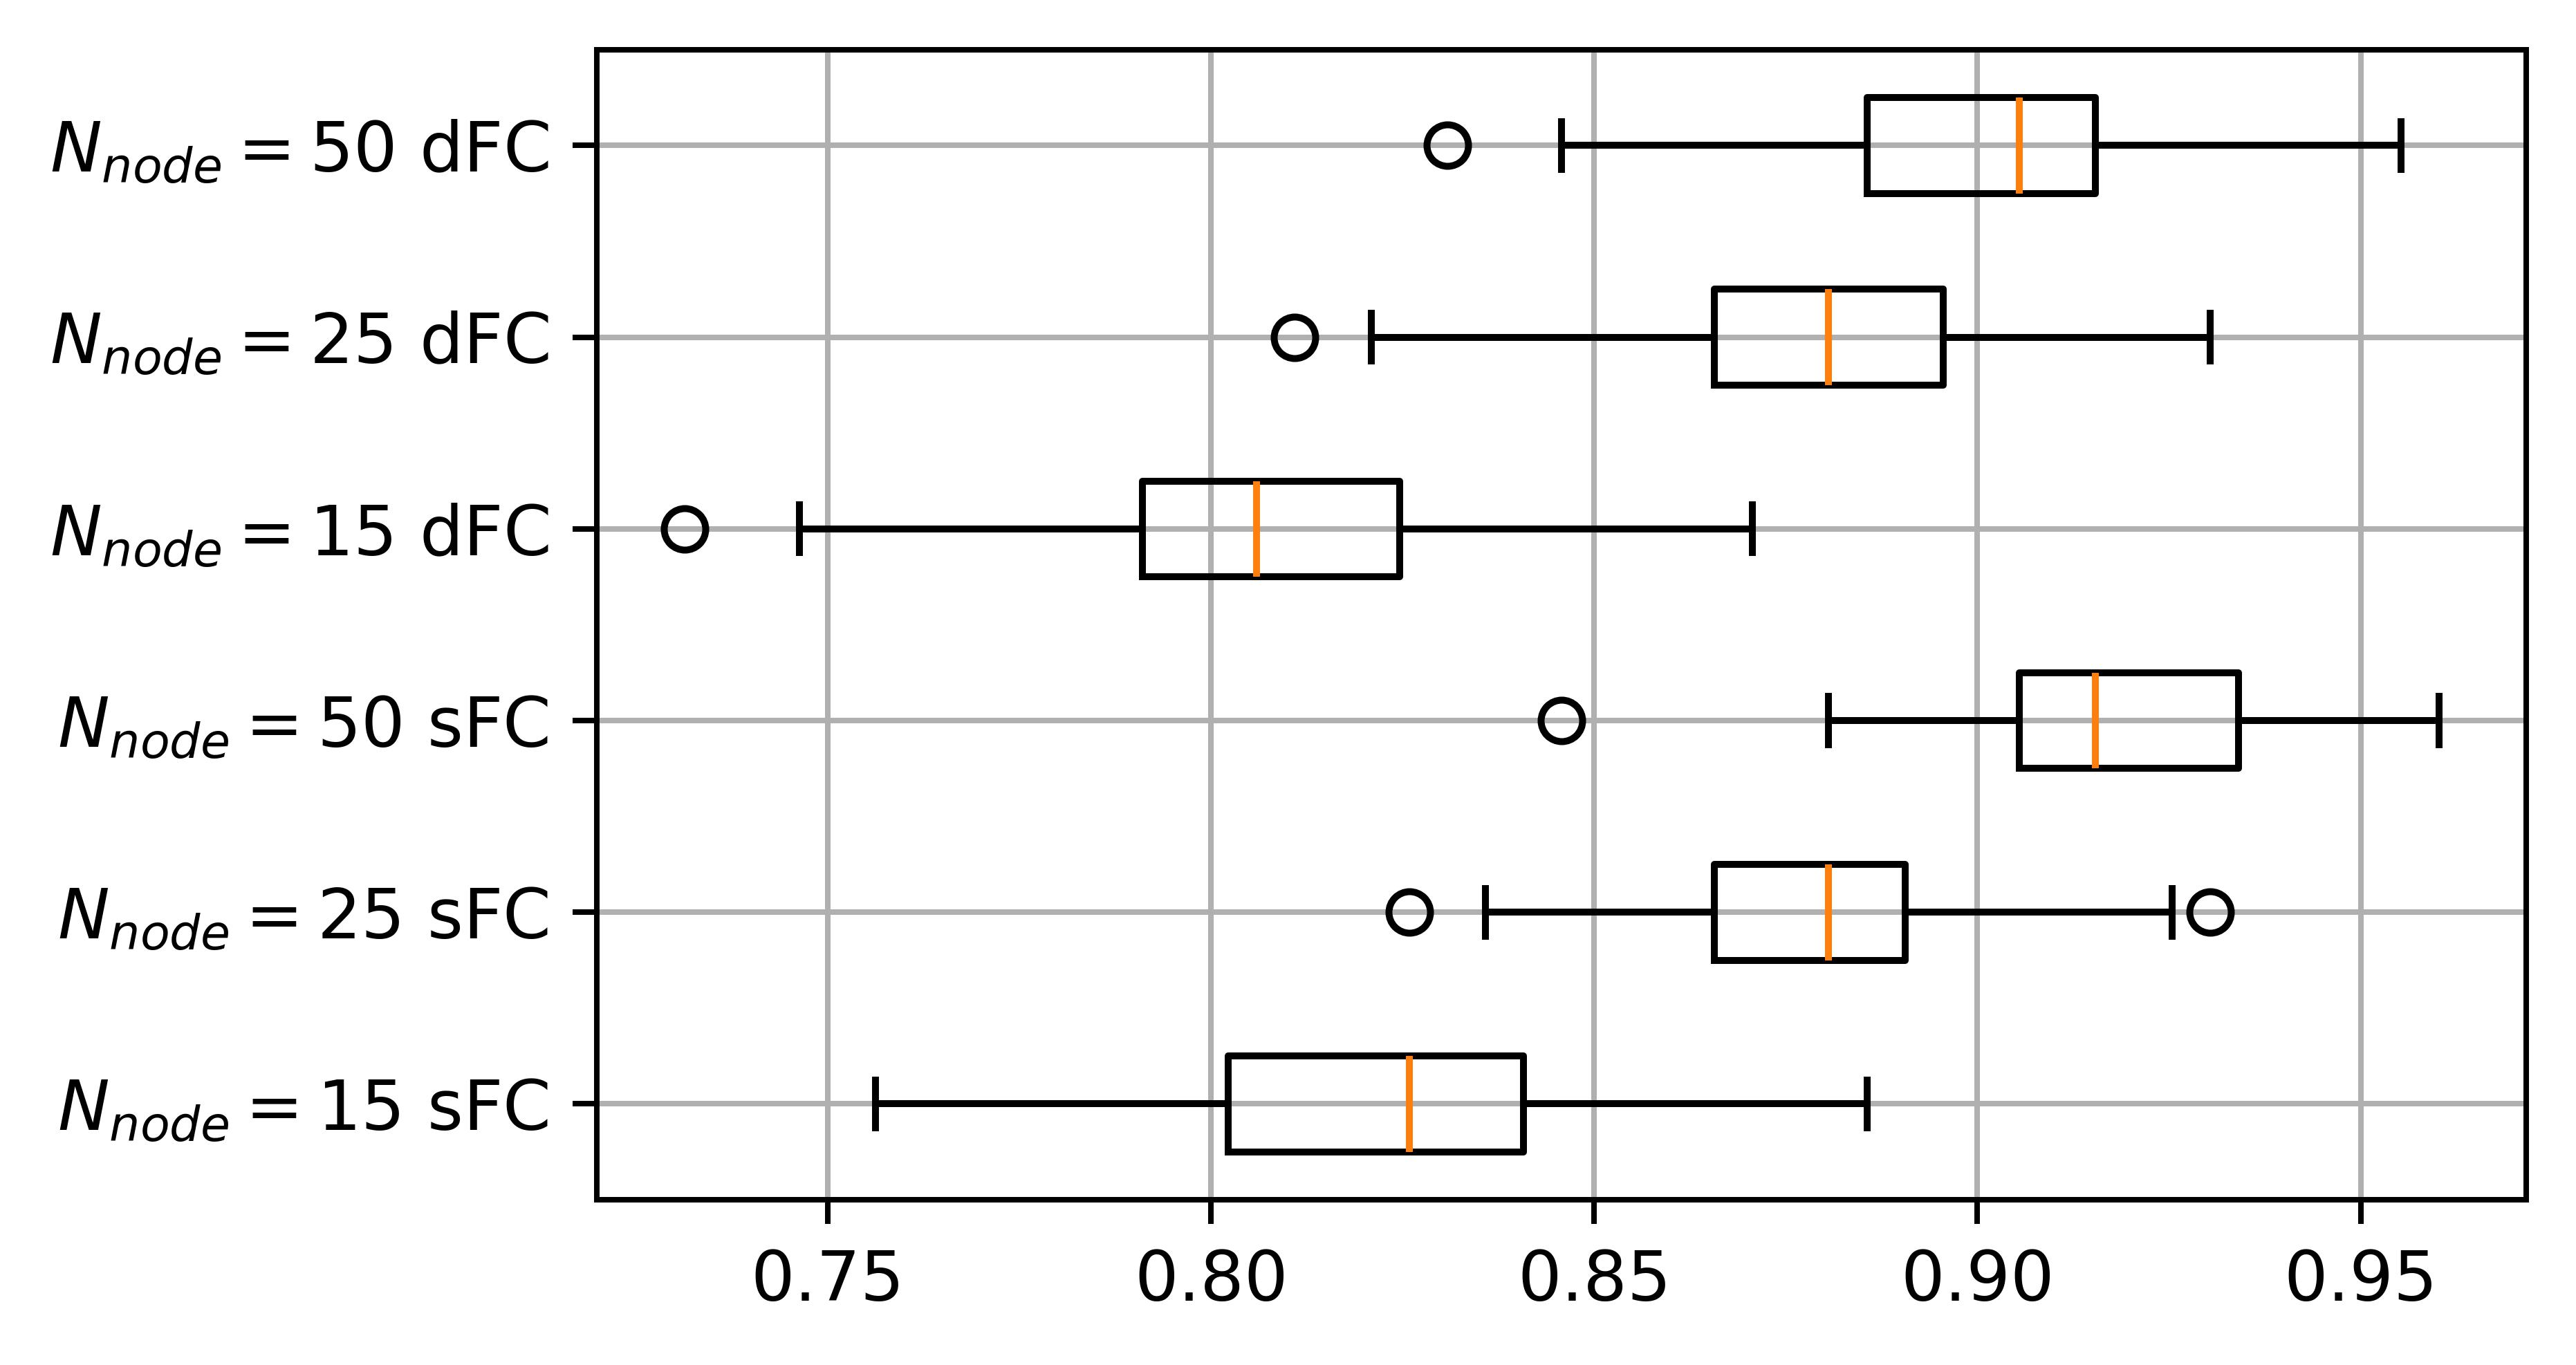
\includegraphics[width=0.4\textwidth]{../SVM/acc_nu_0.1.jpg}}
    \subfloat[test AUC for NuSVM]{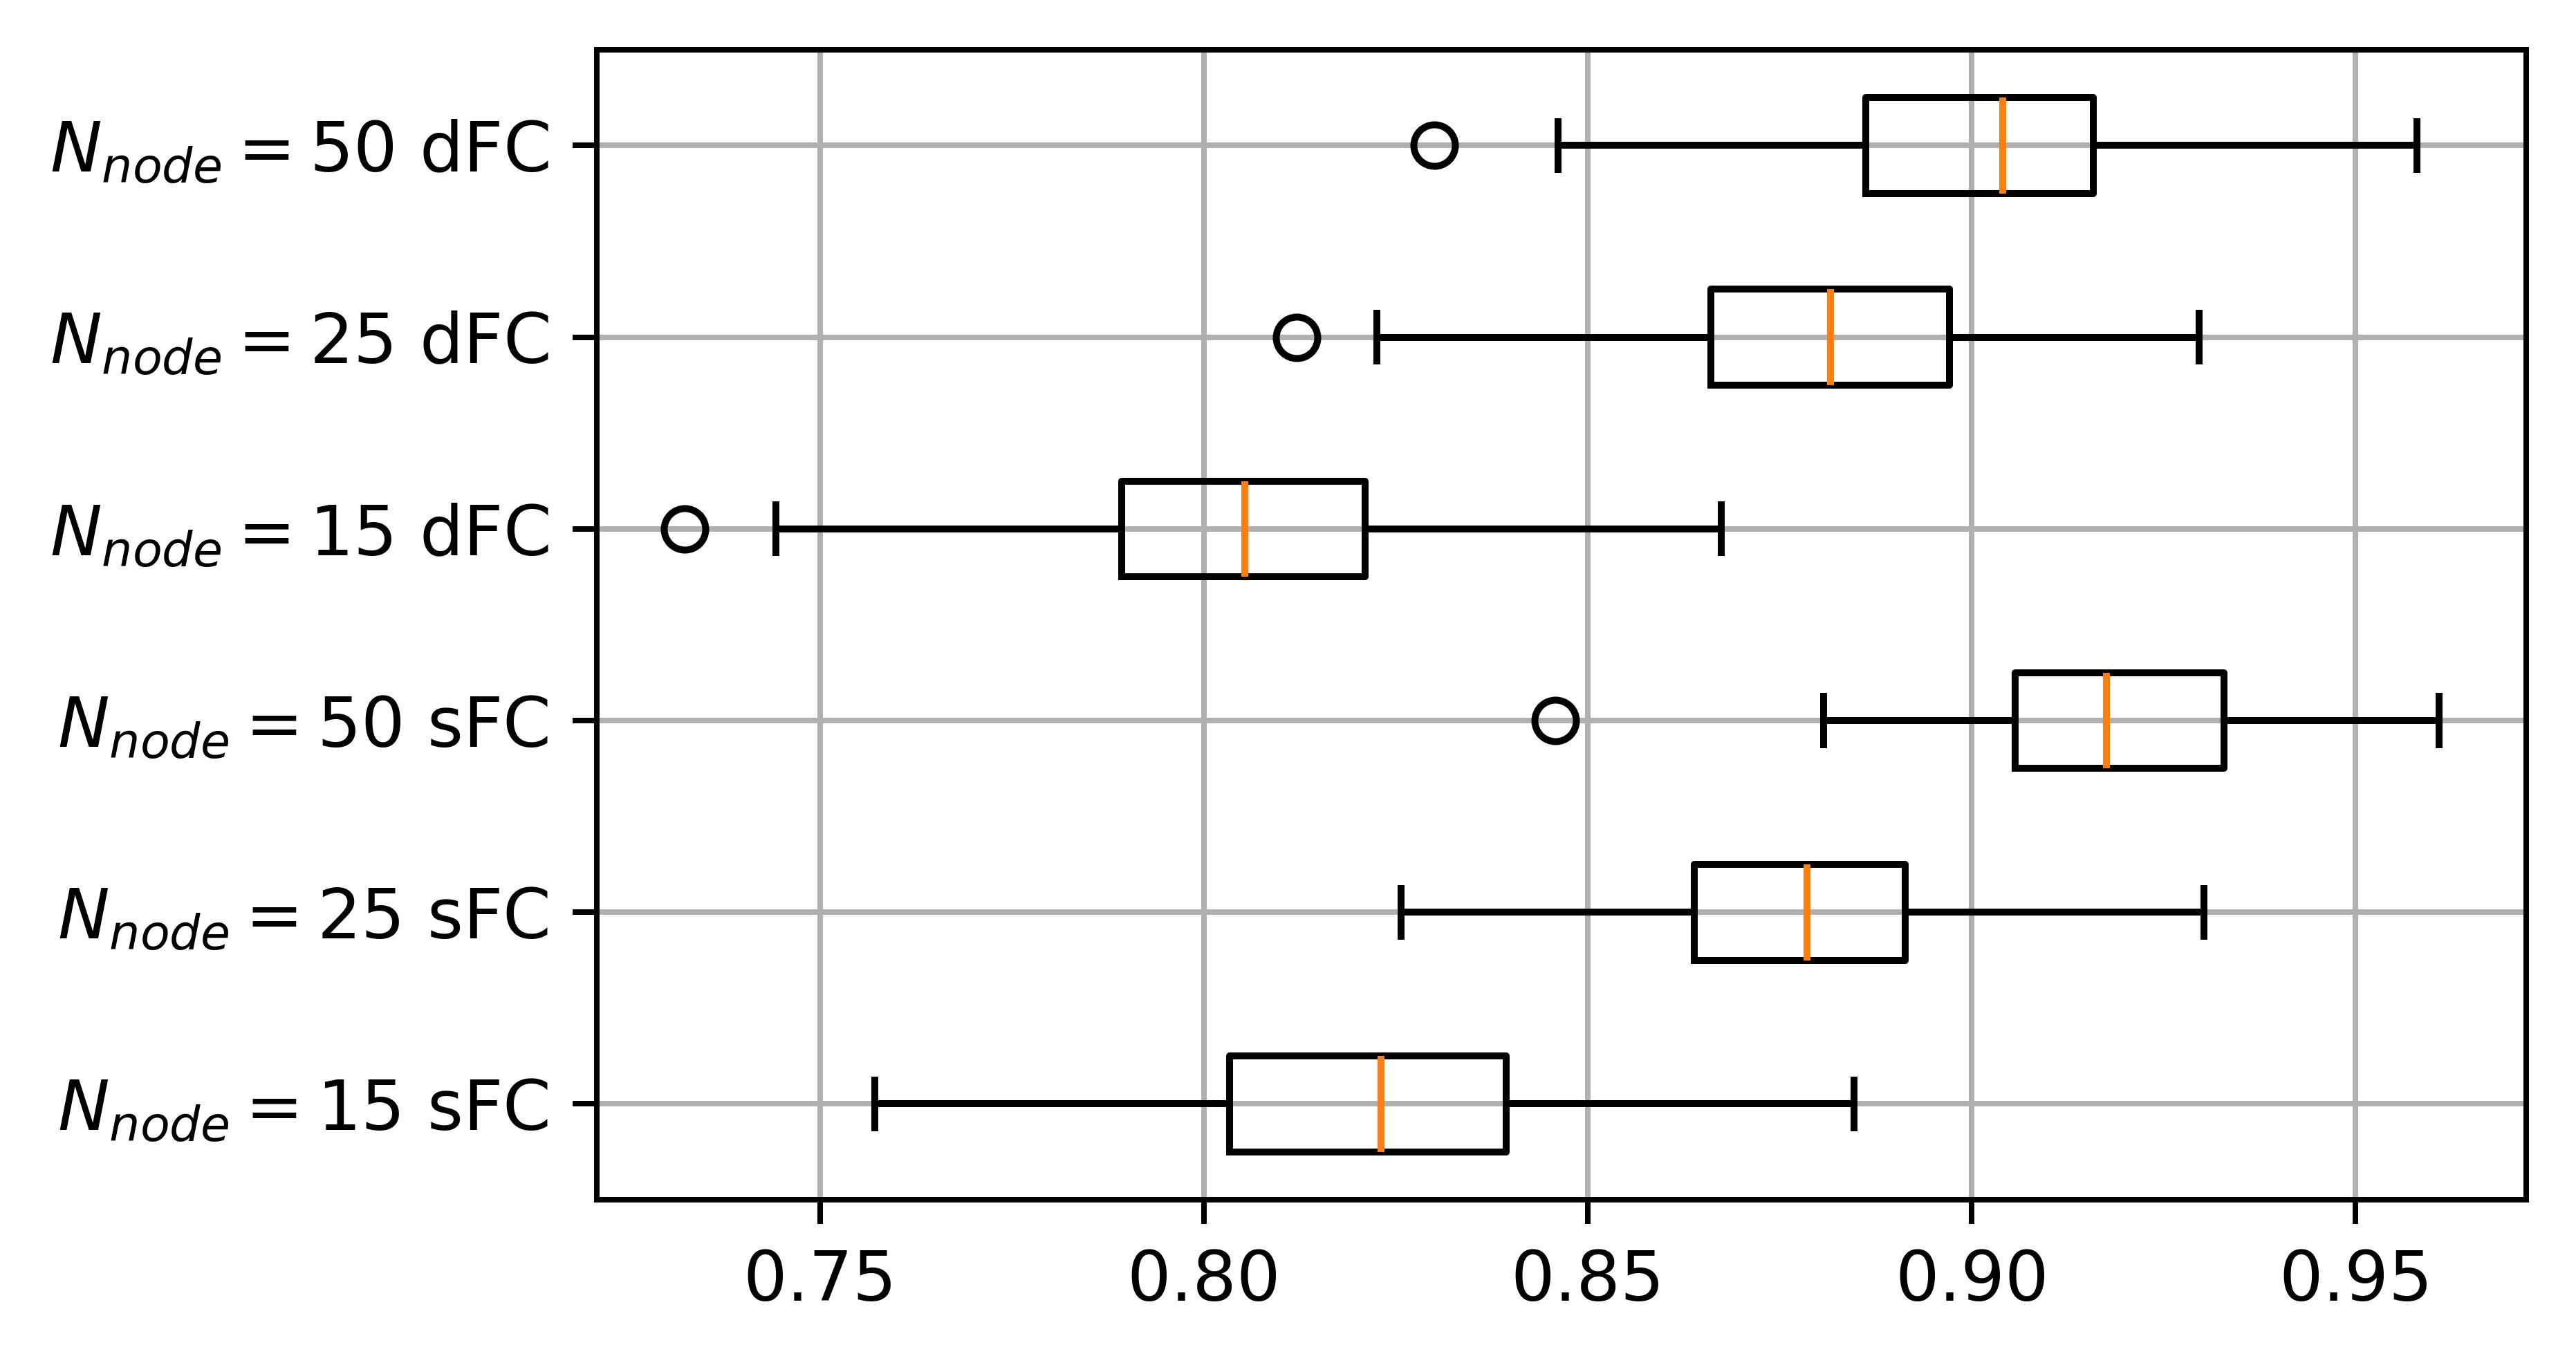
\includegraphics[width=0.4\textwidth]{../SVM/auc_nu_0.1.jpg}} \\
    \caption{Results of SVM.}
\end{figure}

\subsection{Ablation study for CNN model}
\label{Ablation-study-for-CNN-model}

\begin{table}[H]
    \centering
    \begin{tabular}{|c|c|c|c|c|c|}
        \hline
        Data & Dropout & Channel & min ACC/AUC   & mean ACC/AUC  & max ACC/AUC   \\
        \hline
        sFC  & 0.0     & 1       & 0.5224/0.8108 & 0.7957/0.8855 & 0.8706/0.9307 \\
        \hline
        sFC  & 0.0     & 2       & 0.7164/0.8273 & 0.8001/0.8876 & 0.8756/0.9281 \\
        \hline
        sFC  & 0.0     & 4       & 0.7363/0.8189 & 0.7988/0.8863 & 0.8607/0.9337 \\
        \hline
        sFC  & 0.1     & 1       & 0.5174/0.8041 & 0.7952/0.8870 & 0.8756/0.9355 \\
        \hline
        sFC  & 0.1     & 2       & 0.7164/0.8318 & 0.7986/0.8885 & 0.8756/0.9294 \\
        \hline
        sFC  & 0.1     & 4       & 0.7313/0.8276 & 0.8038/0.8911 & 0.8607/0.9317 \\
        \hline
        dFC  & 0.0     & 1       & 0.5871/0.7160 & 0.7737/0.8670 & 0.8557/0.9216 \\
        \hline
        dFC  & 0.0     & 2       & 0.6915/0.7824 & 0.7811/0.8630 & 0.8507/0.9209 \\
        \hline
        dFC  & 0.0     & 4       & 0.7015/0.8028 & 0.7787/0.8584 & 0.8408/0.9148 \\
        \hline
        dFC  & 0.1     & 1       & 0.5522/0.7140 & 0.7735/0.8656 & 0.8458/0.9209 \\
        \hline
        dFC  & 0.1     & 2       & 0.6617/0.7942 & 0.7771/0.8692 & 0.8408/0.9110 \\
        \hline
        dFC  & 0.1     & 4       & 0.7164/0.7987 & 0.7813/0.8666 & 0.8408/0.9171 \\
        \hline
    \end{tabular}
    \caption{Ablation study for $N_{\text{node}} = 15$.}
\end{table}

\begin{table}[H]
    \centering
    \begin{tabular}{|c|c|c|c|c|c|}
        \hline
        Data & Dropout & Channel & min ACC/AUC   & mean ACC/AUC  & max ACC/AUC   \\
        \hline
        sFC  & 0.0     & 1       & 0.5075/0.7475 & 0.8462/0.9265 & 0.9104/0.9634 \\
        \hline
        sFC  & 0.0     & 2       & 0.7662/0.8731 & 0.8470/0.9225 & 0.9104/0.9599 \\
        \hline
        sFC  & 0.0     & 4       & 0.7512/0.8650 & 0.8468/0.9220 & 0.9055/0.9603 \\
        \hline
        sFC  & 0.1     & 1       & 0.5124/0.7431 & 0.8547/0.9356 & 0.9154/0.9688 \\
        \hline
        sFC  & 0.1     & 2       & 0.7711/0.8598 & 0.8581/0.9358 & 0.9254/0.9728 \\
        \hline
        sFC  & 0.1     & 4       & 0.7711/0.8730 & 0.8562/0.9339 & 0.9104/0.9638 \\
        \hline
        dFC  & 0.0     & 1       & 0.6269/0.7168 & 0.8450/0.9338 & 0.9303/0.9788 \\
        \hline
        dFC  & 0.0     & 2       & 0.7463/0.8662 & 0.8594/0.9416 & 0.9254/0.9787 \\
        \hline
        dFC  & 0.0     & 4       & 0.7960/0.9130 & 0.8672/0.9437 & 0.9154/0.9783 \\
        \hline
        dFC  & 0.1     & 1       & 0.5771/0.6996 & 0.8391/0.9319 & 0.9254/0.9753 \\
        \hline
        dFC  & 0.1     & 2       & 0.7612/0.8584 & 0.8618/0.9441 & 0.9204/0.9752 \\
        \hline
        dFC  & 0.1     & 4       & 0.7264/0.8902 & 0.8606/0.9426 & 0.9104/0.9739 \\
        \hline
    \end{tabular}
    \caption{Ablation study for $N_{\text{node}} = 25$.}
\end{table}

\begin{table}[H]
    \centering
    \begin{tabular}{|c|c|c|c|c|c|}
        \hline
        Data & Dropout & Channel & min ACC/AUC   & mean ACC/AUC  & max ACC/AUC   \\
        \hline
        sFC  & 0.0     & 1       & 0.5572/0.7721 & 0.9015/0.9689 & 0.9602/0.9947 \\
        \hline
        sFC  & 0.0     & 2       & 0.7512/0.8462 & 0.9218/0.9762 & 0.9701/0.9941 \\
        \hline
        sFC  & 0.0     & 4       & 0.8856/0.9589 & 0.9248/0.9779 & 0.9602/0.9938 \\
        \hline
        sFC  & 0.1     & 1       & 0.5124/0.7691 & 0.8960/0.9684 & 0.9652/0.9952 \\
        \hline
        sFC  & 0.1     & 2       & 0.7363/0.8335 & 0.9147/0.9746 & 0.9652/0.9947 \\
        \hline
        sFC  & 0.1     & 4       & 0.8358/0.9562 & 0.9178/0.9778 & 0.9652/0.9940 \\
        \hline
        dFC  & 0.0     & 1       & 0.6766/0.8767 & 0.8799/0.9689 & 0.9552/0.9924 \\
        \hline
        dFC  & 0.0     & 2       & 0.7711/0.9366 & 0.9041/0.9733 & 0.9552/0.9917 \\
        \hline
        dFC  & 0.0     & 4       & 0.8507/0.9543 & 0.9122/0.9766 & 0.9602/0.9946 \\
        \hline
        dFC  & 0.1     & 1       & 0.7363/0.8511 & 0.8945/0.9714 & 0.9602/0.9940 \\
        \hline
        dFC  & 0.1     & 2       & 0.8109/0.8966 & 0.9027/0.9716 & 0.9552/0.9925 \\
        \hline
        dFC  & 0.1     & 4       & 0.7711/0.9128 & 0.9040/0.9713 & 0.9552/0.9930 \\
        \hline
    \end{tabular}
    \caption{Ablation study for $N_{\text{node}} = 50$.}
\end{table}

\begin{figure}[H]
    \centering
    \subfloat[test ACC with dropout=0.0]{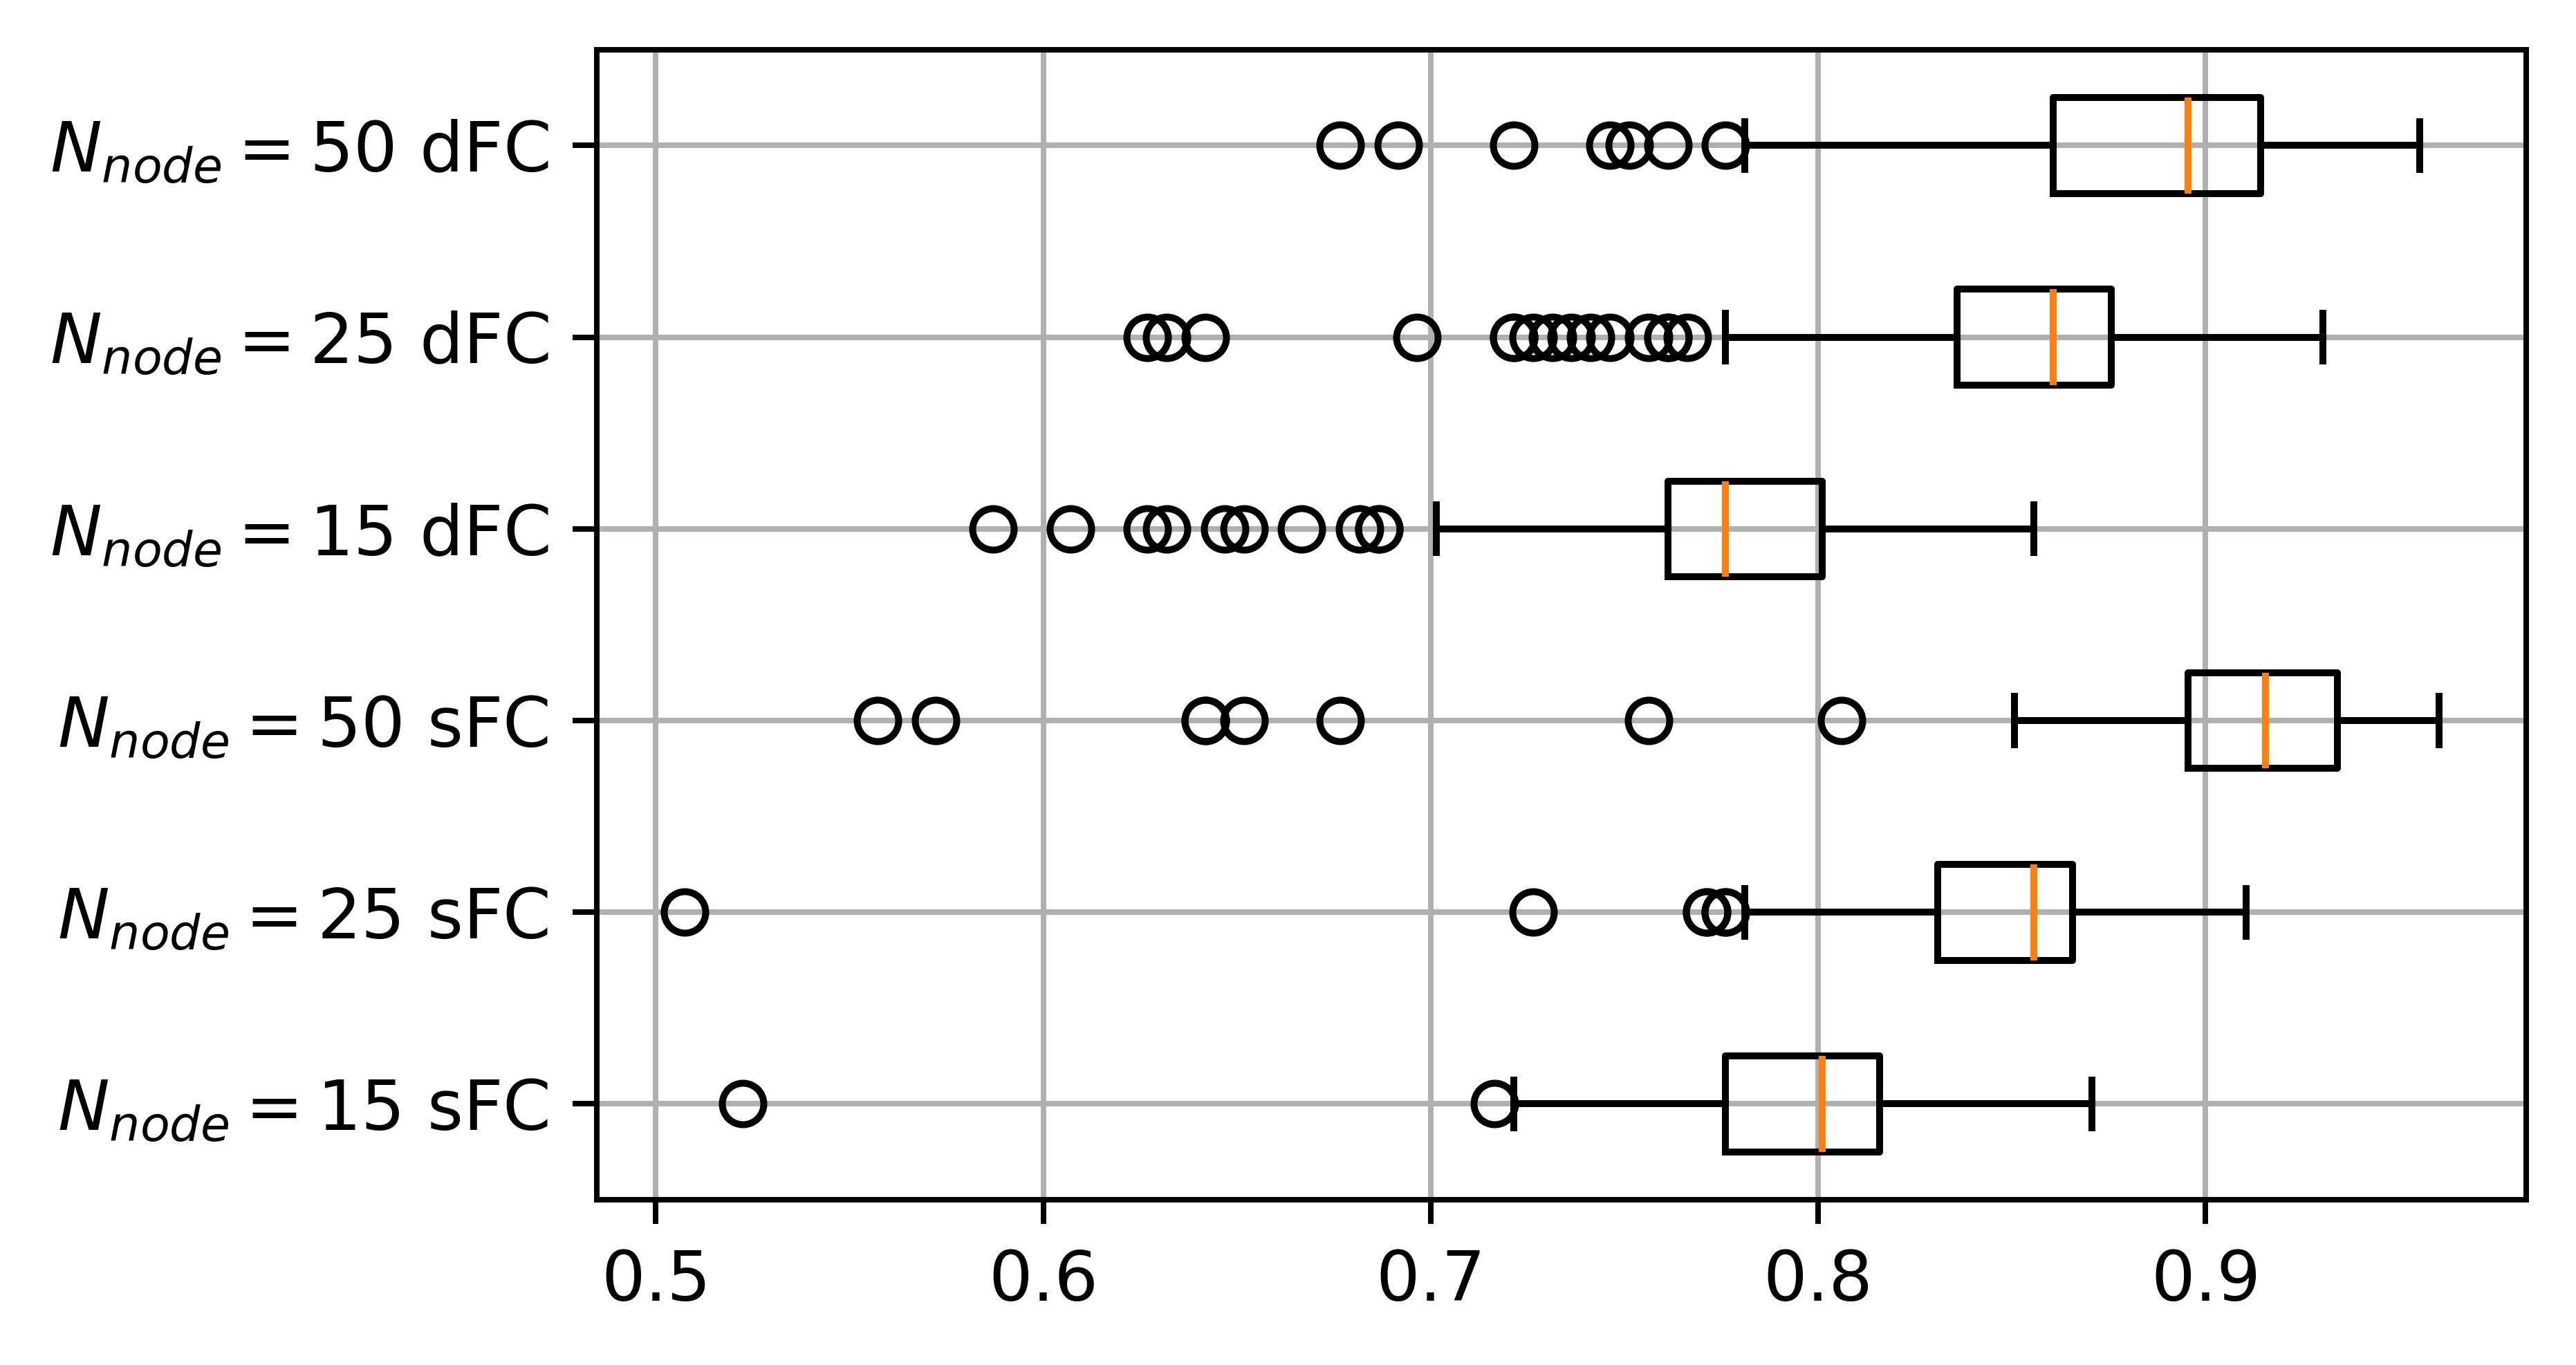
\includegraphics[width=0.4\textwidth]{../Result/test_acc_box_channel=1_dropout=0.0.jpg}}
    \subfloat[test AUC with dropout=0.0]{\includegraphics[width=0.4\textwidth]{../Result/test_auc_box_channel=1_dropout=0.0.jpg}} \\
    \subfloat[test ACC with dropout=0.1]{\includegraphics[width=0.4\textwidth]{../Result/test_acc_box_channel=1_dropout=0.1.jpg}}
    \subfloat[test AUC with dropout=0.1]{\includegraphics[width=0.4\textwidth]{../Result/test_auc_box_channel=1_dropout=0.1.jpg}}
    \caption{Results of CNN model with channel = 1.}
    % \label{CNN-results-3}
\end{figure}

\begin{figure}[H]
    \centering
    \subfloat[test ACC with dropout=0.0]{\includegraphics[width=0.4\textwidth]{../Result/test_acc_box_channel=2_dropout=0.0.jpg}}
    \subfloat[test AUC with dropout=0.0]{\includegraphics[width=0.4\textwidth]{../Result/test_auc_box_channel=2_dropout=0.0.jpg}} \\
    \subfloat[test ACC with dropout=0.1]{\includegraphics[width=0.4\textwidth]{../Result/test_acc_box_channel=2_dropout=0.1.jpg}}
    \subfloat[test AUC with dropout=0.1]{\includegraphics[width=0.4\textwidth]{../Result/test_auc_box_channel=2_dropout=0.1.jpg}}
    \caption{Results of CNN model with channel = 2.}
    % \label{CNN-results-3}
\end{figure}

\begin{figure}[H]
    \centering
    \subfloat[test ACC with dropout=0.0]{\includegraphics[width=0.4\textwidth]{../Result/test_acc_box_channel=4_dropout=0.0.jpg}}
    \subfloat[test AUC with dropout=0.0]{\includegraphics[width=0.4\textwidth]{../Result/test_auc_box_channel=4_dropout=0.0.jpg}} \\
    \subfloat[test ACC with dropout=0.1]{\includegraphics[width=0.4\textwidth]{../Result/test_acc_box_channel=4_dropout=0.1.jpg}}
    \subfloat[test AUC with dropout=0.1]{\includegraphics[width=0.4\textwidth]{../Result/test_auc_box_channel=4_dropout=0.1.jpg}}
    \caption{Results of CNN model with channel = 4.}
    % \label{CNN-results-3}
\end{figure}

\subsection{Analysis for repetitions}

There are multiple choise for repetition times, e.g., in some article, this number is set to $300$\cite{Leming2021-on}. Thus is is neccessary to analysis how this parameter affect the result.

Assume that the results (AUC or ACC) $\{X_i\}_{i=1}^n$ for different test are independent and identically distributed (i.i.d.) with mean value $\mu$ and variance $\sigma^2$, then from central limit theorem

$$
    Y_n = \frac{\sum_{i=1}^n X_i - n \mu}{\sqrt{n} \sigma} \xrightarrow{D} N(0, 1).
$$

Thus for all $\varepsilon > 0$,

$$
    P\left(\vert \bar{X}_i - \mu \vert \leq \frac{\sigma \varepsilon}{\sqrt{n}}\right) = P(\vert Y_n - E(Y_n) \vert \leq \varepsilon) = \varPhi(\varepsilon) - \varPhi(-\varepsilon),
$$

where $\varPhi(x)$ is the cumulative distribution function of the standard normal distribution.

We compute the variance of samples $\sigma \leq \sqrt{0.007} \leq 0.1$, which implies that if choose $\varepsilon = \sqrt{n} / \delta$, then

$$
    P\left(\vert (\bar{X}_i - \mu)\vert \leq \frac{0.1}{\delta}\right) \geq P\left(\vert \bar{X}_i - \mu \vert \leq \frac{\sigma}{\delta}\right) = \varPhi\left(\frac{\sqrt{n}}{\delta}\right) - \varPhi\left(-\frac{\sqrt{n}}{\delta}\right).
$$

Then for $n = 150$, the result is shown as Table \ref{table-a-as-repetitions}, which implies that the results can reaches an error lower than $1\%$.

\begin{table}[H]
    \centering
    \begin{tabular}{|l|l|}
        \hline
        $\delta = 5$    & $P(\vert \bar{X}_i - \mu \vert \leq 0.02) \geq 0.9857$    \\
        \hline
        $\delta = 8$    & $P(\vert \bar{X}_i - \mu \vert \leq 0.0125) \geq 0.8742$  \\
        \hline
        $\delta = 10$   & $P(\vert \bar{X}_i - \mu \vert \leq 0.01) \geq 0.7793$    \\
        \hline
        $\delta = 12.5$ & $P(\vert \bar{X}_i - \mu \vert \leq 0.008) \geq 0.6728$   \\
        \hline
        $\delta = 16$   & $P(\vert \bar{X}_i - \mu \vert \leq 0.00625) \geq 0.5560$ \\
        \hline
        $\delta = 20$   & $P(\vert \bar{X}_i - \mu \vert \leq 0.005) \geq 0.4597$   \\
        \hline
    \end{tabular}
    \caption{Probability of errors.}
    \label{table-a-as-repetitions}
\end{table}

\end{document}